\documentclass[11pt]{article}

    \usepackage[breakable]{tcolorbox}
    \usepackage{parskip} % Stop auto-indenting (to mimic markdown behaviour)
    
    \usepackage{iftex}
    \ifPDFTeX
    	\usepackage[T1]{fontenc}
    	\usepackage{mathpazo}
    \else
    	\usepackage{fontspec}
    \fi
	\usepackage[UTF8]{ctex}
    % Basic figure setup, for now with no caption control since it's done
    % automatically by Pandoc (which extracts ![](path) syntax from Markdown).
    \usepackage{graphicx}
    % Maintain compatibility with old templates. Remove in nbconvert 6.0
    \let\Oldincludegraphics\includegraphics
    % Ensure that by default, figures have no caption (until we provide a
    % proper Figure object with a Caption API and a way to capture that
    % in the conversion process - todo).
    \usepackage{caption}
    \DeclareCaptionFormat{nocaption}{}
    \captionsetup{format=nocaption,aboveskip=0pt,belowskip=0pt}

    \usepackage[Export]{adjustbox} % Used to constrain images to a maximum size
    \adjustboxset{max size={0.9\linewidth}{0.9\paperheight}}
    \usepackage{float}
    \floatplacement{figure}{H} % forces figures to be placed at the correct location
    \usepackage{xcolor} % Allow colors to be defined
    \usepackage{enumerate} % Needed for markdown enumerations to work
    \usepackage{geometry} % Used to adjust the document margins
    \usepackage{amsmath} % Equations
    \usepackage{amssymb} % Equations
    \usepackage{textcomp} % defines textquotesingle
    % Hack from http://tex.stackexchange.com/a/47451/13684:
    \AtBeginDocument{%
        \def\PYZsq{\textquotesingle}% Upright quotes in Pygmentized code
    }
    \usepackage{upquote} % Upright quotes for verbatim code
    \usepackage{eurosym} % defines \euro
    \usepackage[mathletters]{ucs} % Extended unicode (utf-8) support
    \usepackage{fancyvrb} % verbatim replacement that allows latex
    \usepackage{grffile} % extends the file name processing of package graphics 
                         % to support a larger range
    \makeatletter % fix for grffile with XeLaTeX
    \def\Gread@@xetex#1{%
      \IfFileExists{"\Gin@base".bb}%
      {\Gread@eps{\Gin@base.bb}}%
      {\Gread@@xetex@aux#1}%
    }
    \makeatother

    % The hyperref package gives us a pdf with properly built
    % internal navigation ('pdf bookmarks' for the table of contents,
    % internal cross-reference links, web links for URLs, etc.)
    \usepackage{hyperref}
    % The default LaTeX title has an obnoxious amount of whitespace. By default,
    % titling removes some of it. It also provides customization options.
    \usepackage{titling}
    \usepackage{longtable} % longtable support required by pandoc >1.10
    \usepackage{booktabs}  % table support for pandoc > 1.12.2
    \usepackage[inline]{enumitem} % IRkernel/repr support (it uses the enumerate* environment)
    %\usepackage[normalem]{ulem} % ulem is needed to support strikethroughs (\sout)
                                % normalem makes italics be italics, not underlines
    \usepackage{mathrsfs}
    

    
    % Colors for the hyperref package
    \definecolor{urlcolor}{rgb}{0,.145,.698}
    \definecolor{linkcolor}{rgb}{.71,0.21,0.01}
    \definecolor{citecolor}{rgb}{.12,.54,.11}

    % ANSI colors
    \definecolor{ansi-black}{HTML}{3E424D}
    \definecolor{ansi-black-intense}{HTML}{282C36}
    \definecolor{ansi-red}{HTML}{E75C58}
    \definecolor{ansi-red-intense}{HTML}{B22B31}
    \definecolor{ansi-green}{HTML}{00A250}
    \definecolor{ansi-green-intense}{HTML}{007427}
    \definecolor{ansi-yellow}{HTML}{DDB62B}
    \definecolor{ansi-yellow-intense}{HTML}{B27D12}
    \definecolor{ansi-blue}{HTML}{208FFB}
    \definecolor{ansi-blue-intense}{HTML}{0065CA}
    \definecolor{ansi-magenta}{HTML}{D160C4}
    \definecolor{ansi-magenta-intense}{HTML}{A03196}
    \definecolor{ansi-cyan}{HTML}{60C6C8}
    \definecolor{ansi-cyan-intense}{HTML}{258F8F}
    \definecolor{ansi-white}{HTML}{C5C1B4}
    \definecolor{ansi-white-intense}{HTML}{A1A6B2}
    \definecolor{ansi-default-inverse-fg}{HTML}{FFFFFF}
    \definecolor{ansi-default-inverse-bg}{HTML}{000000}

    % commands and environments needed by pandoc snippets
    % extracted from the output of `pandoc -s`
    \providecommand{\tightlist}{%
      \setlength{\itemsep}{0pt}\setlength{\parskip}{0pt}}
    \DefineVerbatimEnvironment{Highlighting}{Verbatim}{commandchars=\\\{\}}
    % Add ',fontsize=\small' for more characters per line
    \newenvironment{Shaded}{}{}
    \newcommand{\KeywordTok}[1]{\textcolor[rgb]{0.00,0.44,0.13}{\textbf{{#1}}}}
    \newcommand{\DataTypeTok}[1]{\textcolor[rgb]{0.56,0.13,0.00}{{#1}}}
    \newcommand{\DecValTok}[1]{\textcolor[rgb]{0.25,0.63,0.44}{{#1}}}
    \newcommand{\BaseNTok}[1]{\textcolor[rgb]{0.25,0.63,0.44}{{#1}}}
    \newcommand{\FloatTok}[1]{\textcolor[rgb]{0.25,0.63,0.44}{{#1}}}
    \newcommand{\CharTok}[1]{\textcolor[rgb]{0.25,0.44,0.63}{{#1}}}
    \newcommand{\StringTok}[1]{\textcolor[rgb]{0.25,0.44,0.63}{{#1}}}
    \newcommand{\CommentTok}[1]{\textcolor[rgb]{0.38,0.63,0.69}{\textit{{#1}}}}
    \newcommand{\OtherTok}[1]{\textcolor[rgb]{0.00,0.44,0.13}{{#1}}}
    \newcommand{\AlertTok}[1]{\textcolor[rgb]{1.00,0.00,0.00}{\textbf{{#1}}}}
    \newcommand{\FunctionTok}[1]{\textcolor[rgb]{0.02,0.16,0.49}{{#1}}}
    \newcommand{\RegionMarkerTok}[1]{{#1}}
    \newcommand{\ErrorTok}[1]{\textcolor[rgb]{1.00,0.00,0.00}{\textbf{{#1}}}}
    \newcommand{\NormalTok}[1]{{#1}}
    
    % Additional commands for more recent versions of Pandoc
    \newcommand{\ConstantTok}[1]{\textcolor[rgb]{0.53,0.00,0.00}{{#1}}}
    \newcommand{\SpecialCharTok}[1]{\textcolor[rgb]{0.25,0.44,0.63}{{#1}}}
    \newcommand{\VerbatimStringTok}[1]{\textcolor[rgb]{0.25,0.44,0.63}{{#1}}}
    \newcommand{\SpecialStringTok}[1]{\textcolor[rgb]{0.73,0.40,0.53}{{#1}}}
    \newcommand{\ImportTok}[1]{{#1}}
    \newcommand{\DocumentationTok}[1]{\textcolor[rgb]{0.73,0.13,0.13}{\textit{{#1}}}}
    \newcommand{\AnnotationTok}[1]{\textcolor[rgb]{0.38,0.63,0.69}{\textbf{\textit{{#1}}}}}
    \newcommand{\CommentVarTok}[1]{\textcolor[rgb]{0.38,0.63,0.69}{\textbf{\textit{{#1}}}}}
    \newcommand{\VariableTok}[1]{\textcolor[rgb]{0.10,0.09,0.49}{{#1}}}
    \newcommand{\ControlFlowTok}[1]{\textcolor[rgb]{0.00,0.44,0.13}{\textbf{{#1}}}}
    \newcommand{\OperatorTok}[1]{\textcolor[rgb]{0.40,0.40,0.40}{{#1}}}
    \newcommand{\BuiltInTok}[1]{{#1}}
    \newcommand{\ExtensionTok}[1]{{#1}}
    \newcommand{\PreprocessorTok}[1]{\textcolor[rgb]{0.74,0.48,0.00}{{#1}}}
    \newcommand{\AttributeTok}[1]{\textcolor[rgb]{0.49,0.56,0.16}{{#1}}}
    \newcommand{\InformationTok}[1]{\textcolor[rgb]{0.38,0.63,0.69}{\textbf{\textit{{#1}}}}}
    \newcommand{\WarningTok}[1]{\textcolor[rgb]{0.38,0.63,0.69}{\textbf{\textit{{#1}}}}}
    
    
    % Define a nice break command that doesn't care if a line doesn't already
    % exist.
    \def\br{\hspace*{\fill} \\* }
    % Math Jax compatibility definitions
    \def\gt{>}
    \def\lt{<}
    \let\Oldtex\TeX
    \let\Oldlatex\LaTeX
    \renewcommand{\TeX}{\textrm{\Oldtex}}
    \renewcommand{\LaTeX}{\textrm{\Oldlatex}}
    % Document parameters
    % Document title
    \title{Untitled}
    
    
    
    
    
% Pygments definitions
\makeatletter
\def\PY@reset{\let\PY@it=\relax \let\PY@bf=\relax%
    \let\PY@ul=\relax \let\PY@tc=\relax%
    \let\PY@bc=\relax \let\PY@ff=\relax}
\def\PY@tok#1{\csname PY@tok@#1\endcsname}
\def\PY@toks#1+{\ifx\relax#1\empty\else%
    \PY@tok{#1}\expandafter\PY@toks\fi}
\def\PY@do#1{\PY@bc{\PY@tc{\PY@ul{%
    \PY@it{\PY@bf{\PY@ff{#1}}}}}}}
\def\PY#1#2{\PY@reset\PY@toks#1+\relax+\PY@do{#2}}

\expandafter\def\csname PY@tok@w\endcsname{\def\PY@tc##1{\textcolor[rgb]{0.73,0.73,0.73}{##1}}}
\expandafter\def\csname PY@tok@c\endcsname{\let\PY@it=\textit\def\PY@tc##1{\textcolor[rgb]{0.25,0.50,0.50}{##1}}}
\expandafter\def\csname PY@tok@cp\endcsname{\def\PY@tc##1{\textcolor[rgb]{0.74,0.48,0.00}{##1}}}
\expandafter\def\csname PY@tok@k\endcsname{\let\PY@bf=\textbf\def\PY@tc##1{\textcolor[rgb]{0.00,0.50,0.00}{##1}}}
\expandafter\def\csname PY@tok@kp\endcsname{\def\PY@tc##1{\textcolor[rgb]{0.00,0.50,0.00}{##1}}}
\expandafter\def\csname PY@tok@kt\endcsname{\def\PY@tc##1{\textcolor[rgb]{0.69,0.00,0.25}{##1}}}
\expandafter\def\csname PY@tok@o\endcsname{\def\PY@tc##1{\textcolor[rgb]{0.40,0.40,0.40}{##1}}}
\expandafter\def\csname PY@tok@ow\endcsname{\let\PY@bf=\textbf\def\PY@tc##1{\textcolor[rgb]{0.67,0.13,1.00}{##1}}}
\expandafter\def\csname PY@tok@nb\endcsname{\def\PY@tc##1{\textcolor[rgb]{0.00,0.50,0.00}{##1}}}
\expandafter\def\csname PY@tok@nf\endcsname{\def\PY@tc##1{\textcolor[rgb]{0.00,0.00,1.00}{##1}}}
\expandafter\def\csname PY@tok@nc\endcsname{\let\PY@bf=\textbf\def\PY@tc##1{\textcolor[rgb]{0.00,0.00,1.00}{##1}}}
\expandafter\def\csname PY@tok@nn\endcsname{\let\PY@bf=\textbf\def\PY@tc##1{\textcolor[rgb]{0.00,0.00,1.00}{##1}}}
\expandafter\def\csname PY@tok@ne\endcsname{\let\PY@bf=\textbf\def\PY@tc##1{\textcolor[rgb]{0.82,0.25,0.23}{##1}}}
\expandafter\def\csname PY@tok@nv\endcsname{\def\PY@tc##1{\textcolor[rgb]{0.10,0.09,0.49}{##1}}}
\expandafter\def\csname PY@tok@no\endcsname{\def\PY@tc##1{\textcolor[rgb]{0.53,0.00,0.00}{##1}}}
\expandafter\def\csname PY@tok@nl\endcsname{\def\PY@tc##1{\textcolor[rgb]{0.63,0.63,0.00}{##1}}}
\expandafter\def\csname PY@tok@ni\endcsname{\let\PY@bf=\textbf\def\PY@tc##1{\textcolor[rgb]{0.60,0.60,0.60}{##1}}}
\expandafter\def\csname PY@tok@na\endcsname{\def\PY@tc##1{\textcolor[rgb]{0.49,0.56,0.16}{##1}}}
\expandafter\def\csname PY@tok@nt\endcsname{\let\PY@bf=\textbf\def\PY@tc##1{\textcolor[rgb]{0.00,0.50,0.00}{##1}}}
\expandafter\def\csname PY@tok@nd\endcsname{\def\PY@tc##1{\textcolor[rgb]{0.67,0.13,1.00}{##1}}}
\expandafter\def\csname PY@tok@s\endcsname{\def\PY@tc##1{\textcolor[rgb]{0.73,0.13,0.13}{##1}}}
\expandafter\def\csname PY@tok@sd\endcsname{\let\PY@it=\textit\def\PY@tc##1{\textcolor[rgb]{0.73,0.13,0.13}{##1}}}
\expandafter\def\csname PY@tok@si\endcsname{\let\PY@bf=\textbf\def\PY@tc##1{\textcolor[rgb]{0.73,0.40,0.53}{##1}}}
\expandafter\def\csname PY@tok@se\endcsname{\let\PY@bf=\textbf\def\PY@tc##1{\textcolor[rgb]{0.73,0.40,0.13}{##1}}}
\expandafter\def\csname PY@tok@sr\endcsname{\def\PY@tc##1{\textcolor[rgb]{0.73,0.40,0.53}{##1}}}
\expandafter\def\csname PY@tok@ss\endcsname{\def\PY@tc##1{\textcolor[rgb]{0.10,0.09,0.49}{##1}}}
\expandafter\def\csname PY@tok@sx\endcsname{\def\PY@tc##1{\textcolor[rgb]{0.00,0.50,0.00}{##1}}}
\expandafter\def\csname PY@tok@m\endcsname{\def\PY@tc##1{\textcolor[rgb]{0.40,0.40,0.40}{##1}}}
\expandafter\def\csname PY@tok@gh\endcsname{\let\PY@bf=\textbf\def\PY@tc##1{\textcolor[rgb]{0.00,0.00,0.50}{##1}}}
\expandafter\def\csname PY@tok@gu\endcsname{\let\PY@bf=\textbf\def\PY@tc##1{\textcolor[rgb]{0.50,0.00,0.50}{##1}}}
\expandafter\def\csname PY@tok@gd\endcsname{\def\PY@tc##1{\textcolor[rgb]{0.63,0.00,0.00}{##1}}}
\expandafter\def\csname PY@tok@gi\endcsname{\def\PY@tc##1{\textcolor[rgb]{0.00,0.63,0.00}{##1}}}
\expandafter\def\csname PY@tok@gr\endcsname{\def\PY@tc##1{\textcolor[rgb]{1.00,0.00,0.00}{##1}}}
\expandafter\def\csname PY@tok@ge\endcsname{\let\PY@it=\textit}
\expandafter\def\csname PY@tok@gs\endcsname{\let\PY@bf=\textbf}
\expandafter\def\csname PY@tok@gp\endcsname{\let\PY@bf=\textbf\def\PY@tc##1{\textcolor[rgb]{0.00,0.00,0.50}{##1}}}
\expandafter\def\csname PY@tok@go\endcsname{\def\PY@tc##1{\textcolor[rgb]{0.53,0.53,0.53}{##1}}}
\expandafter\def\csname PY@tok@gt\endcsname{\def\PY@tc##1{\textcolor[rgb]{0.00,0.27,0.87}{##1}}}
\expandafter\def\csname PY@tok@err\endcsname{\def\PY@bc##1{\setlength{\fboxsep}{0pt}\fcolorbox[rgb]{1.00,0.00,0.00}{1,1,1}{\strut ##1}}}
\expandafter\def\csname PY@tok@kc\endcsname{\let\PY@bf=\textbf\def\PY@tc##1{\textcolor[rgb]{0.00,0.50,0.00}{##1}}}
\expandafter\def\csname PY@tok@kd\endcsname{\let\PY@bf=\textbf\def\PY@tc##1{\textcolor[rgb]{0.00,0.50,0.00}{##1}}}
\expandafter\def\csname PY@tok@kn\endcsname{\let\PY@bf=\textbf\def\PY@tc##1{\textcolor[rgb]{0.00,0.50,0.00}{##1}}}
\expandafter\def\csname PY@tok@kr\endcsname{\let\PY@bf=\textbf\def\PY@tc##1{\textcolor[rgb]{0.00,0.50,0.00}{##1}}}
\expandafter\def\csname PY@tok@bp\endcsname{\def\PY@tc##1{\textcolor[rgb]{0.00,0.50,0.00}{##1}}}
\expandafter\def\csname PY@tok@fm\endcsname{\def\PY@tc##1{\textcolor[rgb]{0.00,0.00,1.00}{##1}}}
\expandafter\def\csname PY@tok@vc\endcsname{\def\PY@tc##1{\textcolor[rgb]{0.10,0.09,0.49}{##1}}}
\expandafter\def\csname PY@tok@vg\endcsname{\def\PY@tc##1{\textcolor[rgb]{0.10,0.09,0.49}{##1}}}
\expandafter\def\csname PY@tok@vi\endcsname{\def\PY@tc##1{\textcolor[rgb]{0.10,0.09,0.49}{##1}}}
\expandafter\def\csname PY@tok@vm\endcsname{\def\PY@tc##1{\textcolor[rgb]{0.10,0.09,0.49}{##1}}}
\expandafter\def\csname PY@tok@sa\endcsname{\def\PY@tc##1{\textcolor[rgb]{0.73,0.13,0.13}{##1}}}
\expandafter\def\csname PY@tok@sb\endcsname{\def\PY@tc##1{\textcolor[rgb]{0.73,0.13,0.13}{##1}}}
\expandafter\def\csname PY@tok@sc\endcsname{\def\PY@tc##1{\textcolor[rgb]{0.73,0.13,0.13}{##1}}}
\expandafter\def\csname PY@tok@dl\endcsname{\def\PY@tc##1{\textcolor[rgb]{0.73,0.13,0.13}{##1}}}
\expandafter\def\csname PY@tok@s2\endcsname{\def\PY@tc##1{\textcolor[rgb]{0.73,0.13,0.13}{##1}}}
\expandafter\def\csname PY@tok@sh\endcsname{\def\PY@tc##1{\textcolor[rgb]{0.73,0.13,0.13}{##1}}}
\expandafter\def\csname PY@tok@s1\endcsname{\def\PY@tc##1{\textcolor[rgb]{0.73,0.13,0.13}{##1}}}
\expandafter\def\csname PY@tok@mb\endcsname{\def\PY@tc##1{\textcolor[rgb]{0.40,0.40,0.40}{##1}}}
\expandafter\def\csname PY@tok@mf\endcsname{\def\PY@tc##1{\textcolor[rgb]{0.40,0.40,0.40}{##1}}}
\expandafter\def\csname PY@tok@mh\endcsname{\def\PY@tc##1{\textcolor[rgb]{0.40,0.40,0.40}{##1}}}
\expandafter\def\csname PY@tok@mi\endcsname{\def\PY@tc##1{\textcolor[rgb]{0.40,0.40,0.40}{##1}}}
\expandafter\def\csname PY@tok@il\endcsname{\def\PY@tc##1{\textcolor[rgb]{0.40,0.40,0.40}{##1}}}
\expandafter\def\csname PY@tok@mo\endcsname{\def\PY@tc##1{\textcolor[rgb]{0.40,0.40,0.40}{##1}}}
\expandafter\def\csname PY@tok@ch\endcsname{\let\PY@it=\textit\def\PY@tc##1{\textcolor[rgb]{0.25,0.50,0.50}{##1}}}
\expandafter\def\csname PY@tok@cm\endcsname{\let\PY@it=\textit\def\PY@tc##1{\textcolor[rgb]{0.25,0.50,0.50}{##1}}}
\expandafter\def\csname PY@tok@cpf\endcsname{\let\PY@it=\textit\def\PY@tc##1{\textcolor[rgb]{0.25,0.50,0.50}{##1}}}
\expandafter\def\csname PY@tok@c1\endcsname{\let\PY@it=\textit\def\PY@tc##1{\textcolor[rgb]{0.25,0.50,0.50}{##1}}}
\expandafter\def\csname PY@tok@cs\endcsname{\let\PY@it=\textit\def\PY@tc##1{\textcolor[rgb]{0.25,0.50,0.50}{##1}}}

\def\PYZbs{\char`\\}
\def\PYZus{\char`\_}
\def\PYZob{\char`\{}
\def\PYZcb{\char`\}}
\def\PYZca{\char`\^}
\def\PYZam{\char`\&}
\def\PYZlt{\char`\<}
\def\PYZgt{\char`\>}
\def\PYZsh{\char`\#}
\def\PYZpc{\char`\%}
\def\PYZdl{\char`\$}
\def\PYZhy{\char`\-}
\def\PYZsq{\char`\'}
\def\PYZdq{\char`\"}
\def\PYZti{\char`\~}
% for compatibility with earlier versions
\def\PYZat{@}
\def\PYZlb{[}
\def\PYZrb{]}
\makeatother


    % For linebreaks inside Verbatim environment from package fancyvrb. 
    \makeatletter
        \newbox\Wrappedcontinuationbox 
        \newbox\Wrappedvisiblespacebox 
        \newcommand*\Wrappedvisiblespace {\textcolor{red}{\textvisiblespace}} 
        \newcommand*\Wrappedcontinuationsymbol {\textcolor{red}{\llap{\tiny$\m@th\hookrightarrow$}}} 
        \newcommand*\Wrappedcontinuationindent {3ex } 
        \newcommand*\Wrappedafterbreak {\kern\Wrappedcontinuationindent\copy\Wrappedcontinuationbox} 
        % Take advantage of the already applied Pygments mark-up to insert 
        % potential linebreaks for TeX processing. 
        %        {, <, #, %, $, ' and ": go to next line. 
        %        _, }, ^, &, >, - and ~: stay at end of broken line. 
        % Use of \textquotesingle for straight quote. 
        \newcommand*\Wrappedbreaksatspecials {% 
            \def\PYGZus{\discretionary{\char`\_}{\Wrappedafterbreak}{\char`\_}}% 
            \def\PYGZob{\discretionary{}{\Wrappedafterbreak\char`\{}{\char`\{}}% 
            \def\PYGZcb{\discretionary{\char`\}}{\Wrappedafterbreak}{\char`\}}}% 
            \def\PYGZca{\discretionary{\char`\^}{\Wrappedafterbreak}{\char`\^}}% 
            \def\PYGZam{\discretionary{\char`\&}{\Wrappedafterbreak}{\char`\&}}% 
            \def\PYGZlt{\discretionary{}{\Wrappedafterbreak\char`\<}{\char`\<}}% 
            \def\PYGZgt{\discretionary{\char`\>}{\Wrappedafterbreak}{\char`\>}}% 
            \def\PYGZsh{\discretionary{}{\Wrappedafterbreak\char`\#}{\char`\#}}% 
            \def\PYGZpc{\discretionary{}{\Wrappedafterbreak\char`\%}{\char`\%}}% 
            \def\PYGZdl{\discretionary{}{\Wrappedafterbreak\char`\$}{\char`\$}}% 
            \def\PYGZhy{\discretionary{\char`\-}{\Wrappedafterbreak}{\char`\-}}% 
            \def\PYGZsq{\discretionary{}{\Wrappedafterbreak\textquotesingle}{\textquotesingle}}% 
            \def\PYGZdq{\discretionary{}{\Wrappedafterbreak\char`\"}{\char`\"}}% 
            \def\PYGZti{\discretionary{\char`\~}{\Wrappedafterbreak}{\char`\~}}% 
        } 
        % Some characters . , ; ? ! / are not pygmentized. 
        % This macro makes them "active" and they will insert potential linebreaks 
        \newcommand*\Wrappedbreaksatpunct {% 
            \lccode`\~`\.\lowercase{\def~}{\discretionary{\hbox{\char`\.}}{\Wrappedafterbreak}{\hbox{\char`\.}}}% 
            \lccode`\~`\,\lowercase{\def~}{\discretionary{\hbox{\char`\,}}{\Wrappedafterbreak}{\hbox{\char`\,}}}% 
            \lccode`\~`\;\lowercase{\def~}{\discretionary{\hbox{\char`\;}}{\Wrappedafterbreak}{\hbox{\char`\;}}}% 
            \lccode`\~`\:\lowercase{\def~}{\discretionary{\hbox{\char`\:}}{\Wrappedafterbreak}{\hbox{\char`\:}}}% 
            \lccode`\~`\?\lowercase{\def~}{\discretionary{\hbox{\char`\?}}{\Wrappedafterbreak}{\hbox{\char`\?}}}% 
            \lccode`\~`\!\lowercase{\def~}{\discretionary{\hbox{\char`\!}}{\Wrappedafterbreak}{\hbox{\char`\!}}}% 
            \lccode`\~`\/\lowercase{\def~}{\discretionary{\hbox{\char`\/}}{\Wrappedafterbreak}{\hbox{\char`\/}}}% 
            \catcode`\.\active
            \catcode`\,\active 
            \catcode`\;\active
            \catcode`\:\active
            \catcode`\?\active
            \catcode`\!\active
            \catcode`\/\active 
            \lccode`\~`\~ 	
        }
    \makeatother

    \let\OriginalVerbatim=\Verbatim
    \makeatletter
    \renewcommand{\Verbatim}[1][1]{%
        %\parskip\z@skip
        \sbox\Wrappedcontinuationbox {\Wrappedcontinuationsymbol}%
        \sbox\Wrappedvisiblespacebox {\FV@SetupFont\Wrappedvisiblespace}%
        \def\FancyVerbFormatLine ##1{\hsize\linewidth
            \vtop{\raggedright\hyphenpenalty\z@\exhyphenpenalty\z@
                \doublehyphendemerits\z@\finalhyphendemerits\z@
                \strut ##1\strut}%
        }%
        % If the linebreak is at a space, the latter will be displayed as visible
        % space at end of first line, and a continuation symbol starts next line.
        % Stretch/shrink are however usually zero for typewriter font.
        \def\FV@Space {%
            \nobreak\hskip\z@ plus\fontdimen3\font minus\fontdimen4\font
            \discretionary{\copy\Wrappedvisiblespacebox}{\Wrappedafterbreak}
            {\kern\fontdimen2\font}%
        }%
        
        % Allow breaks at special characters using \PYG... macros.
        \Wrappedbreaksatspecials
        % Breaks at punctuation characters . , ; ? ! and / need catcode=\active 	
        \OriginalVerbatim[#1,codes*=\Wrappedbreaksatpunct]%
    }
    \makeatother

    % Exact colors from NB
    \definecolor{incolor}{HTML}{303F9F}
    \definecolor{outcolor}{HTML}{D84315}
    \definecolor{cellborder}{HTML}{CFCFCF}
    \definecolor{cellbackground}{HTML}{F7F7F7}
    
    % prompt
    \makeatletter
    \newcommand{\boxspacing}{\kern\kvtcb@left@rule\kern\kvtcb@boxsep}
    \makeatother
    \newcommand{\prompt}[4]{
        \ttfamily\llap{{\color{#2}[#3]:\hspace{3pt}#4}}\vspace{-\baselineskip}
    }
    

    
    % Prevent overflowing lines due to hard-to-break entities
    \sloppy 
    % Setup hyperref package
    \hypersetup{
      breaklinks=true,  % so long urls are correctly broken across lines
      colorlinks=true,
      urlcolor=urlcolor,
      linkcolor=linkcolor,
      citecolor=citecolor,
      }
    % Slightly bigger margins than the latex defaults
    
    \geometry{verbose,tmargin=1in,bmargin=1in,lmargin=1in,rmargin=1in}
    
    

\begin{document}
    
    %\maketitle
    
    

    
    \hypertarget{ux4f5cux4e1aux6e05ux5355420}{%
\section{作业清单(4/20)}\label{ux4f5cux4e1aux6e05ux5355420}}

    \hypertarget{ux95eeux9898ux4e00-ux73afux5883ux5b89ux88c5}{%
\subsection{问题一
环境安装}\label{ux95eeux9898ux4e00-ux73afux5883ux5b89ux88c5}}

    【1】 安装Python 3.X 和 Orange3 软件,是否完成?

    \textbf{回答:}已完成

    \begin{tcolorbox}[breakable, size=fbox, boxrule=1pt, pad at break*=1mm,colback=cellbackground, colframe=cellborder]
\prompt{In}{incolor}{131}{\boxspacing}
\begin{Verbatim}[commandchars=\\\{\}]
\PY{k+kn}{import} \PY{n+nn}{Orange}
\PY{n}{data} \PY{o}{=} \PY{n}{Orange}\PY{o}{.}\PY{n}{data}\PY{o}{.}\PY{n}{Table}\PY{p}{(}\PY{l+s+s2}{\PYZdq{}}\PY{l+s+s2}{iris}\PY{l+s+s2}{\PYZdq{}}\PY{p}{)}

\PY{n+nb}{print}\PY{p}{(}\PY{l+s+s2}{\PYZdq{}}\PY{l+s+s2}{Attributes}\PY{l+s+s2}{\PYZdq{}}\PY{p}{,}\PY{l+s+s2}{\PYZdq{}}\PY{l+s+s2}{,}\PY{l+s+s2}{\PYZdq{}}\PY{o}{.}\PY{n}{join}\PY{p}{(}\PY{n}{x}\PY{o}{.}\PY{n}{name} \PY{k}{for} \PY{n}{x} \PY{o+ow}{in} \PY{n}{data}\PY{o}{.}\PY{n}{domain}\PY{o}{.}\PY{n}{attributes}\PY{p}{)}\PY{p}{)}
\end{Verbatim}
\end{tcolorbox}

    \begin{Verbatim}[commandchars=\\\{\}]
Attributes sepal length,sepal width,petal length,petal width
    \end{Verbatim}

    \hypertarget{ux95eeux9898ux4e8c-ux6559ux5e08ux8eabux4efdux5224ux65adux5b9eux9a8c}{%
\subsection{问题二
教师身份判断实验}\label{ux95eeux9898ux4e8c-ux6559ux5e08ux8eabux4efdux5224ux65adux5b9eux9a8c}}

    【2】 完成课堂实验(给定教师数据,判断身份的实验),是否完成?

    \textbf{回答:}已完成

    \begin{tcolorbox}[breakable, size=fbox, boxrule=1pt, pad at break*=1mm,colback=cellbackground, colframe=cellborder]
\prompt{In}{incolor}{3}{\boxspacing}
\begin{Verbatim}[commandchars=\\\{\}]
\PY{c+c1}{\PYZsh{} 给定数据集}
\PY{n}{test\PYZus{}data} \PY{o}{=} \PY{p}{\PYZob{}}\PY{l+s+s1}{\PYZsq{}}\PY{l+s+s1}{Tom}\PY{l+s+s1}{\PYZsq{}}\PY{p}{:} \PY{p}{\PYZob{}}\PY{l+s+s1}{\PYZsq{}}\PY{l+s+s1}{RANK}\PY{l+s+s1}{\PYZsq{}}\PY{p}{:} \PY{l+s+s1}{\PYZsq{}}\PY{l+s+s1}{A1}\PY{l+s+s1}{\PYZsq{}}\PY{p}{,} \PY{l+s+s1}{\PYZsq{}}\PY{l+s+s1}{YEARS}\PY{l+s+s1}{\PYZsq{}}\PY{p}{:} \PY{l+m+mi}{2}\PY{p}{,} \PY{l+s+s1}{\PYZsq{}}\PY{l+s+s1}{TENURED}\PY{l+s+s1}{\PYZsq{}}\PY{p}{:} \PY{l+s+s1}{\PYZsq{}}\PY{l+s+s1}{N}\PY{l+s+s1}{\PYZsq{}}\PY{p}{\PYZcb{}}\PY{p}{,}
             \PY{l+s+s1}{\PYZsq{}}\PY{l+s+s1}{Merlisa}\PY{l+s+s1}{\PYZsq{}}\PY{p}{:} \PY{p}{\PYZob{}}\PY{l+s+s1}{\PYZsq{}}\PY{l+s+s1}{RANK}\PY{l+s+s1}{\PYZsq{}}\PY{p}{:} \PY{l+s+s1}{\PYZsq{}}\PY{l+s+s1}{A2}\PY{l+s+s1}{\PYZsq{}}\PY{p}{,} \PY{l+s+s1}{\PYZsq{}}\PY{l+s+s1}{YEARS}\PY{l+s+s1}{\PYZsq{}}\PY{p}{:} \PY{l+m+mi}{7}\PY{p}{,} \PY{l+s+s1}{\PYZsq{}}\PY{l+s+s1}{TENURED}\PY{l+s+s1}{\PYZsq{}}\PY{p}{:} \PY{l+s+s1}{\PYZsq{}}\PY{l+s+s1}{N}\PY{l+s+s1}{\PYZsq{}}\PY{p}{\PYZcb{}}\PY{p}{,}
             \PY{l+s+s1}{\PYZsq{}}\PY{l+s+s1}{George}\PY{l+s+s1}{\PYZsq{}}\PY{p}{:} \PY{p}{\PYZob{}}\PY{l+s+s1}{\PYZsq{}}\PY{l+s+s1}{RANK}\PY{l+s+s1}{\PYZsq{}}\PY{p}{:} \PY{l+s+s1}{\PYZsq{}}\PY{l+s+s1}{P}\PY{l+s+s1}{\PYZsq{}}\PY{p}{,} \PY{l+s+s1}{\PYZsq{}}\PY{l+s+s1}{YEARS}\PY{l+s+s1}{\PYZsq{}}\PY{p}{:} \PY{l+m+mi}{5}\PY{p}{,} \PY{l+s+s1}{\PYZsq{}}\PY{l+s+s1}{TENURED}\PY{l+s+s1}{\PYZsq{}}\PY{p}{:} \PY{l+s+s1}{\PYZsq{}}\PY{l+s+s1}{Y}\PY{l+s+s1}{\PYZsq{}}\PY{p}{\PYZcb{}}\PY{p}{,}
             \PY{l+s+s1}{\PYZsq{}}\PY{l+s+s1}{Joseph}\PY{l+s+s1}{\PYZsq{}}\PY{p}{:} \PY{p}{\PYZob{}}\PY{l+s+s1}{\PYZsq{}}\PY{l+s+s1}{RANK}\PY{l+s+s1}{\PYZsq{}}\PY{p}{:} \PY{l+s+s1}{\PYZsq{}}\PY{l+s+s1}{A1}\PY{l+s+s1}{\PYZsq{}}\PY{p}{,} \PY{l+s+s1}{\PYZsq{}}\PY{l+s+s1}{YEARS}\PY{l+s+s1}{\PYZsq{}}\PY{p}{:} \PY{l+m+mi}{7}\PY{p}{,} \PY{l+s+s1}{\PYZsq{}}\PY{l+s+s1}{TENURED}\PY{l+s+s1}{\PYZsq{}}\PY{p}{:} \PY{l+s+s1}{\PYZsq{}}\PY{l+s+s1}{Y}\PY{l+s+s1}{\PYZsq{}}\PY{p}{\PYZcb{}}\PY{p}{\PYZcb{}}
\end{Verbatim}
\end{tcolorbox}

    \begin{tcolorbox}[breakable, size=fbox, boxrule=1pt, pad at break*=1mm,colback=cellbackground, colframe=cellborder]
\prompt{In}{incolor}{4}{\boxspacing}
\begin{Verbatim}[commandchars=\\\{\}]
\PY{c+c1}{\PYZsh{} 给定新的数据}
\PY{n}{name} \PY{o}{=} \PY{l+s+s2}{\PYZdq{}}\PY{l+s+s2}{TQ}\PY{l+s+s2}{\PYZdq{}}
\PY{n}{rank} \PY{o}{=} \PY{l+s+s2}{\PYZdq{}}\PY{l+s+s2}{A1}\PY{l+s+s2}{\PYZdq{}}
\PY{n}{year} \PY{o}{=} \PY{l+m+mi}{10}
\PY{n}{result} \PY{o}{=} \PY{l+s+s2}{\PYZdq{}}\PY{l+s+s2}{N}\PY{l+s+s2}{\PYZdq{}}

\PY{c+c1}{\PYZsh{} 交互式输入数据}
\PY{c+c1}{\PYZsh{} name = input(\PYZdq{}What is your name?\PYZdq{})}
\PY{c+c1}{\PYZsh{} rank = input(\PYZdq{}What is your rank?\PYZdq{})}
\PY{c+c1}{\PYZsh{} year = int(input(\PYZdq{}What is your year?\PYZdq{}))}
\PY{c+c1}{\PYZsh{} result = \PYZsq{}N\PYZsq{}}
\end{Verbatim}
\end{tcolorbox}

    \begin{tcolorbox}[breakable, size=fbox, boxrule=1pt, pad at break*=1mm,colback=cellbackground, colframe=cellborder]
\prompt{In}{incolor}{12}{\boxspacing}
\begin{Verbatim}[commandchars=\\\{\}]
\PY{c+c1}{\PYZsh{} m 用来记录是否生成了该职位的规则,c 用来记录规则}
\PY{n}{c} \PY{o}{=} \PY{p}{\PYZob{}}\PY{p}{\PYZcb{}}
\PY{n}{m} \PY{o}{=} \PY{p}{\PYZob{}}\PY{l+s+s1}{\PYZsq{}}\PY{l+s+s1}{P}\PY{l+s+s1}{\PYZsq{}}\PY{p}{:} \PY{k+kc}{False}\PY{p}{,} \PY{l+s+s1}{\PYZsq{}}\PY{l+s+s1}{A1}\PY{l+s+s1}{\PYZsq{}}\PY{p}{:} \PY{k+kc}{False}\PY{p}{,} \PY{l+s+s1}{\PYZsq{}}\PY{l+s+s1}{A2}\PY{l+s+s1}{\PYZsq{}}\PY{p}{:} \PY{k+kc}{False}\PY{p}{\PYZcb{}}

\PY{c+c1}{\PYZsh{} 找到某一职称下的终身职位的工作年限最小值,作为该职称的分类规则}
\PY{c+c1}{\PYZsh{} 若该职称无终身职位数据,则记录为未发现规则,并将工作年限最大值作为作为可能的分类规则}
\PY{k}{for} \PY{n}{key}\PY{p}{,} \PY{n}{value} \PY{o+ow}{in} \PY{n}{test\PYZus{}data}\PY{o}{.}\PY{n}{items}\PY{p}{(}\PY{p}{)}\PY{p}{:}
    \PY{k}{if} \PY{n}{value}\PY{p}{[}\PY{l+s+s1}{\PYZsq{}}\PY{l+s+s1}{TENURED}\PY{l+s+s1}{\PYZsq{}}\PY{p}{]} \PY{o}{==} \PY{l+s+s1}{\PYZsq{}}\PY{l+s+s1}{Y}\PY{l+s+s1}{\PYZsq{}}\PY{p}{:}
        \PY{k}{if} \PY{n+nb}{len}\PY{p}{(}\PY{n}{c}\PY{p}{)} \PY{o}{==} \PY{l+m+mi}{0}\PY{p}{:}
            \PY{n}{c}\PY{p}{[}\PY{n}{value}\PY{p}{[}\PY{l+s+s1}{\PYZsq{}}\PY{l+s+s1}{RANK}\PY{l+s+s1}{\PYZsq{}}\PY{p}{]}\PY{p}{]} \PY{o}{=} \PY{n}{value}\PY{p}{[}\PY{l+s+s1}{\PYZsq{}}\PY{l+s+s1}{YEARS}\PY{l+s+s1}{\PYZsq{}}\PY{p}{]}
        \PY{k}{else}\PY{p}{:}
            \PY{k}{if} \PY{n}{value}\PY{p}{[}\PY{l+s+s1}{\PYZsq{}}\PY{l+s+s1}{RANK}\PY{l+s+s1}{\PYZsq{}}\PY{p}{]} \PY{o+ow}{not} \PY{o+ow}{in} \PY{n}{c}\PY{o}{.}\PY{n}{keys}\PY{p}{(}\PY{p}{)}\PY{p}{:}
                \PY{n}{c}\PY{p}{[}\PY{n}{value}\PY{p}{[}\PY{l+s+s1}{\PYZsq{}}\PY{l+s+s1}{RANK}\PY{l+s+s1}{\PYZsq{}}\PY{p}{]}\PY{p}{]} \PY{o}{=} \PY{n}{value}\PY{p}{[}\PY{l+s+s1}{\PYZsq{}}\PY{l+s+s1}{YEARS}\PY{l+s+s1}{\PYZsq{}}\PY{p}{]}
            \PY{k}{else}\PY{p}{:}
                \PY{k}{if} \PY{n}{c}\PY{p}{[}\PY{n}{value}\PY{p}{[}\PY{l+s+s1}{\PYZsq{}}\PY{l+s+s1}{RANK}\PY{l+s+s1}{\PYZsq{}}\PY{p}{]}\PY{p}{]} \PY{o}{\PYZgt{}} \PY{n}{value}\PY{p}{[}\PY{l+s+s1}{\PYZsq{}}\PY{l+s+s1}{YEARS}\PY{l+s+s1}{\PYZsq{}}\PY{p}{]}\PY{p}{:}
                    \PY{n}{c}\PY{p}{[}\PY{n}{value}\PY{p}{[}\PY{l+s+s1}{\PYZsq{}}\PY{l+s+s1}{RANK}\PY{l+s+s1}{\PYZsq{}}\PY{p}{]}\PY{p}{]} \PY{o}{=} \PY{n}{value}\PY{p}{[}\PY{l+s+s1}{\PYZsq{}}\PY{l+s+s1}{YEARS}\PY{l+s+s1}{\PYZsq{}}\PY{p}{]}
        \PY{n}{m}\PY{p}{[}\PY{n}{value}\PY{p}{[}\PY{l+s+s1}{\PYZsq{}}\PY{l+s+s1}{RANK}\PY{l+s+s1}{\PYZsq{}}\PY{p}{]}\PY{p}{]} \PY{o}{=} \PY{k+kc}{True}
    \PY{k}{else}\PY{p}{:}
        \PY{k}{if} \PY{n+nb}{len}\PY{p}{(}\PY{n}{c}\PY{p}{)} \PY{o}{==} \PY{l+m+mi}{0}\PY{p}{:}
            \PY{n}{c}\PY{p}{[}\PY{n}{value}\PY{p}{[}\PY{l+s+s1}{\PYZsq{}}\PY{l+s+s1}{RANK}\PY{l+s+s1}{\PYZsq{}}\PY{p}{]}\PY{p}{]} \PY{o}{=} \PY{n}{value}\PY{p}{[}\PY{l+s+s1}{\PYZsq{}}\PY{l+s+s1}{YEARS}\PY{l+s+s1}{\PYZsq{}}\PY{p}{]}
        \PY{k}{else}\PY{p}{:}
            \PY{k}{if} \PY{n}{value}\PY{p}{[}\PY{l+s+s1}{\PYZsq{}}\PY{l+s+s1}{RANK}\PY{l+s+s1}{\PYZsq{}}\PY{p}{]} \PY{o+ow}{not} \PY{o+ow}{in} \PY{n}{c}\PY{o}{.}\PY{n}{keys}\PY{p}{(}\PY{p}{)}\PY{p}{:}
                \PY{n}{c}\PY{p}{[}\PY{n}{value}\PY{p}{[}\PY{l+s+s1}{\PYZsq{}}\PY{l+s+s1}{RANK}\PY{l+s+s1}{\PYZsq{}}\PY{p}{]}\PY{p}{]} \PY{o}{=} \PY{n}{value}\PY{p}{[}\PY{l+s+s1}{\PYZsq{}}\PY{l+s+s1}{YEARS}\PY{l+s+s1}{\PYZsq{}}\PY{p}{]}
            \PY{k}{else}\PY{p}{:}
                \PY{k}{if} \PY{n}{c}\PY{p}{[}\PY{n}{value}\PY{p}{[}\PY{l+s+s1}{\PYZsq{}}\PY{l+s+s1}{RANK}\PY{l+s+s1}{\PYZsq{}}\PY{p}{]}\PY{p}{]} \PY{o}{\PYZlt{}} \PY{n}{value}\PY{p}{[}\PY{l+s+s1}{\PYZsq{}}\PY{l+s+s1}{YEARS}\PY{l+s+s1}{\PYZsq{}}\PY{p}{]}\PY{p}{:}
                    \PY{n}{c}\PY{p}{[}\PY{n}{value}\PY{p}{[}\PY{l+s+s1}{\PYZsq{}}\PY{l+s+s1}{RANK}\PY{l+s+s1}{\PYZsq{}}\PY{p}{]}\PY{p}{]} \PY{o}{=} \PY{n}{value}\PY{p}{[}\PY{l+s+s1}{\PYZsq{}}\PY{l+s+s1}{YEARS}\PY{l+s+s1}{\PYZsq{}}\PY{p}{]}
\end{Verbatim}
\end{tcolorbox}

    \begin{tcolorbox}[breakable, size=fbox, boxrule=1pt, pad at break*=1mm,colback=cellbackground, colframe=cellborder]
\prompt{In}{incolor}{13}{\boxspacing}
\begin{Verbatim}[commandchars=\\\{\}]
\PY{n}{m}
\end{Verbatim}
\end{tcolorbox}

            \begin{tcolorbox}[breakable, size=fbox, boxrule=.5pt, pad at break*=1mm, opacityfill=0]
\prompt{Out}{outcolor}{13}{\boxspacing}
\begin{Verbatim}[commandchars=\\\{\}]
\{'P': True, 'A1': True, 'A2': False\}
\end{Verbatim}
\end{tcolorbox}
        
    \begin{tcolorbox}[breakable, size=fbox, boxrule=1pt, pad at break*=1mm,colback=cellbackground, colframe=cellborder]
\prompt{In}{incolor}{14}{\boxspacing}
\begin{Verbatim}[commandchars=\\\{\}]
\PY{n}{c}
\end{Verbatim}
\end{tcolorbox}

            \begin{tcolorbox}[breakable, size=fbox, boxrule=.5pt, pad at break*=1mm, opacityfill=0]
\prompt{Out}{outcolor}{14}{\boxspacing}
\begin{Verbatim}[commandchars=\\\{\}]
\{'A1': 2, 'A2': 7, 'P': 5\}
\end{Verbatim}
\end{tcolorbox}
        
    \begin{tcolorbox}[breakable, size=fbox, boxrule=1pt, pad at break*=1mm,colback=cellbackground, colframe=cellborder]
\prompt{In}{incolor}{17}{\boxspacing}
\begin{Verbatim}[commandchars=\\\{\}]
\PY{c+c1}{\PYZsh{} 若测试数据岗位有规则,按照规则分类}
\PY{c+c1}{\PYZsh{} 否则若工作年限大于给定数据最大值,暂时判定为终身职位}
\PY{k}{if} \PY{n}{m}\PY{p}{[}\PY{n}{rank}\PY{p}{]}\PY{p}{:}
    \PY{k}{if} \PY{n}{year} \PY{o}{\PYZgt{}}\PY{o}{=} \PY{n}{c}\PY{p}{[}\PY{n}{rank}\PY{p}{]}\PY{p}{:}
        \PY{n}{result} \PY{o}{=} \PY{l+s+s1}{\PYZsq{}}\PY{l+s+s1}{Y}\PY{l+s+s1}{\PYZsq{}}
\PY{k}{else}\PY{p}{:}
    \PY{k}{if} \PY{n}{year} \PY{o}{\PYZgt{}} \PY{n}{c}\PY{p}{[}\PY{n}{rank}\PY{p}{]}\PY{p}{:}
        \PY{n}{result} \PY{o}{=} \PY{l+s+s1}{\PYZsq{}}\PY{l+s+s1}{Y}\PY{l+s+s1}{\PYZsq{}}

\PY{k}{if} \PY{n}{result} \PY{o}{==} \PY{l+s+s1}{\PYZsq{}}\PY{l+s+s1}{Y}\PY{l+s+s1}{\PYZsq{}}\PY{p}{:}
    \PY{n+nb}{print}\PY{p}{(}\PY{l+s+s2}{\PYZdq{}}\PY{l+s+s2}{You are TENURED}\PY{l+s+s2}{\PYZdq{}}\PY{p}{)}
\PY{k}{else}\PY{p}{:}
    \PY{n+nb}{print}\PY{p}{(}\PY{l+s+s2}{\PYZdq{}}\PY{l+s+s2}{You aren}\PY{l+s+s2}{\PYZsq{}}\PY{l+s+s2}{t TENURED}\PY{l+s+s2}{\PYZdq{}}\PY{p}{)}
\end{Verbatim}
\end{tcolorbox}

    \begin{Verbatim}[commandchars=\\\{\}]
You are TENURED
    \end{Verbatim}

    \hypertarget{ux95eeux9898ux4e09-ux590dux4e60-numpy}{%
\subsection{问题三 复习
Numpy}\label{ux95eeux9898ux4e09-ux590dux4e60-numpy}}

    【3】 复习Numpy的主要功能(按照课堂PPT完成相关实验)

    \begin{tcolorbox}[breakable, size=fbox, boxrule=1pt, pad at break*=1mm,colback=cellbackground, colframe=cellborder]
\prompt{In}{incolor}{21}{\boxspacing}
\begin{Verbatim}[commandchars=\\\{\}]
\PY{k+kn}{import} \PY{n+nn}{numpy} \PY{k}{as} \PY{n+nn}{np}
\PY{c+c1}{\PYZsh{} ndarray}
\PY{n}{a} \PY{o}{=} \PY{n}{np}\PY{o}{.}\PY{n}{array}\PY{p}{(}\PY{p}{[}\PY{l+m+mi}{1}\PY{p}{,} \PY{l+m+mi}{2}\PY{p}{,} \PY{l+m+mi}{3}\PY{p}{,} \PY{l+m+mi}{4}\PY{p}{]}\PY{p}{)}
\PY{n}{b} \PY{o}{=} \PY{n}{np}\PY{o}{.}\PY{n}{array}\PY{p}{(}\PY{p}{(}\PY{l+m+mi}{5}\PY{p}{,} \PY{l+m+mi}{6}\PY{p}{,} \PY{l+m+mi}{7}\PY{p}{,} \PY{l+m+mi}{8}\PY{p}{)}\PY{p}{)}
\PY{n}{c} \PY{o}{=} \PY{n}{np}\PY{o}{.}\PY{n}{array}\PY{p}{(}\PY{p}{[}\PY{p}{[}\PY{l+m+mi}{1}\PY{p}{,} \PY{l+m+mi}{2}\PY{p}{,} \PY{l+m+mi}{3}\PY{p}{,} \PY{l+m+mi}{4}\PY{p}{]}\PY{p}{,} \PY{p}{[}\PY{l+m+mi}{5}\PY{p}{,} \PY{l+m+mi}{6}\PY{p}{,} \PY{l+m+mi}{7}\PY{p}{,} \PY{l+m+mi}{8}\PY{p}{]}\PY{p}{]}\PY{p}{)}
\end{Verbatim}
\end{tcolorbox}

    \begin{tcolorbox}[breakable, size=fbox, boxrule=1pt, pad at break*=1mm,colback=cellbackground, colframe=cellborder]
\prompt{In}{incolor}{22}{\boxspacing}
\begin{Verbatim}[commandchars=\\\{\}]
\PY{n}{a}\PY{p}{,}\PY{n}{b}\PY{p}{,}\PY{n}{c}
\end{Verbatim}
\end{tcolorbox}

            \begin{tcolorbox}[breakable, size=fbox, boxrule=.5pt, pad at break*=1mm, opacityfill=0]
\prompt{Out}{outcolor}{22}{\boxspacing}
\begin{Verbatim}[commandchars=\\\{\}]
(array([1, 2, 3, 4]), array([5, 6, 7, 8]), array([[1, 2, 3, 4],
        [5, 6, 7, 8]]))
\end{Verbatim}
\end{tcolorbox}
        
    \begin{tcolorbox}[breakable, size=fbox, boxrule=1pt, pad at break*=1mm,colback=cellbackground, colframe=cellborder]
\prompt{In}{incolor}{25}{\boxspacing}
\begin{Verbatim}[commandchars=\\\{\}]
\PY{c+c1}{\PYZsh{} arange 的用法,生成取值在 [start,stop) 范围内步长为 step 的列表}
\PY{n}{a} \PY{o}{=} \PY{n}{np}\PY{o}{.}\PY{n}{arange}\PY{p}{(}\PY{l+m+mi}{0}\PY{p}{,} \PY{l+m+mi}{1}\PY{p}{,} \PY{l+m+mf}{0.1}\PY{p}{)}
\PY{n}{a}
\end{Verbatim}
\end{tcolorbox}

            \begin{tcolorbox}[breakable, size=fbox, boxrule=.5pt, pad at break*=1mm, opacityfill=0]
\prompt{Out}{outcolor}{25}{\boxspacing}
\begin{Verbatim}[commandchars=\\\{\}]
array([0. , 0.1, 0.2, 0.3, 0.4, 0.5, 0.6, 0.7, 0.8, 0.9])
\end{Verbatim}
\end{tcolorbox}
        
    \begin{tcolorbox}[breakable, size=fbox, boxrule=1pt, pad at break*=1mm,colback=cellbackground, colframe=cellborder]
\prompt{In}{incolor}{27}{\boxspacing}
\begin{Verbatim}[commandchars=\\\{\}]
\PY{c+c1}{\PYZsh{} linspace 的用法,生成取值在 [start,stop) 范围内等分的 num 个数}
\PY{n}{b} \PY{o}{=} \PY{n}{np}\PY{o}{.}\PY{n}{linspace}\PY{p}{(}\PY{l+m+mi}{0}\PY{p}{,} \PY{l+m+mi}{1}\PY{p}{,} \PY{l+m+mi}{10}\PY{p}{)}
\PY{n}{b}
\end{Verbatim}
\end{tcolorbox}

            \begin{tcolorbox}[breakable, size=fbox, boxrule=.5pt, pad at break*=1mm, opacityfill=0]
\prompt{Out}{outcolor}{27}{\boxspacing}
\begin{Verbatim}[commandchars=\\\{\}]
array([0.        , 0.11111111, 0.22222222, 0.33333333, 0.44444444,
       0.55555556, 0.66666667, 0.77777778, 0.88888889, 1.        ])
\end{Verbatim}
\end{tcolorbox}
        
    \begin{tcolorbox}[breakable, size=fbox, boxrule=1pt, pad at break*=1mm,colback=cellbackground, colframe=cellborder]
\prompt{In}{incolor}{29}{\boxspacing}
\begin{Verbatim}[commandchars=\\\{\}]
\PY{c+c1}{\PYZsh{} 广播}
\PY{n}{c} \PY{o}{=} \PY{n}{np}\PY{o}{.}\PY{n}{arange}\PY{p}{(}\PY{l+m+mi}{3}\PY{p}{)}
\PY{n}{d} \PY{o}{=} \PY{n}{np}\PY{o}{.}\PY{n}{arange}\PY{p}{(}\PY{l+m+mi}{3}\PY{p}{)}\PY{o}{+}\PY{l+m+mi}{5}
\PY{n}{c}\PY{p}{,}\PY{n}{d}
\end{Verbatim}
\end{tcolorbox}

            \begin{tcolorbox}[breakable, size=fbox, boxrule=.5pt, pad at break*=1mm, opacityfill=0]
\prompt{Out}{outcolor}{29}{\boxspacing}
\begin{Verbatim}[commandchars=\\\{\}]
(array([0, 1, 2]), array([5, 6, 7]))
\end{Verbatim}
\end{tcolorbox}
        
    \hypertarget{ux95eeux9898ux56db-ux6559ux6750ux4e60ux9898}{%
\subsection{问题四
教材习题}\label{ux95eeux9898ux56db-ux6559ux6750ux4e60ux9898}}

    【4】 完成参考教材第1章 1.9的第1题和第4题(抄题)

    1.什么是数据挖掘?在你的回答中,强调以下问题:

    数据挖掘是从大量数据中``挖掘''有趣的信息或模式以能够基于该决策做出决策的过程或方法。

    \begin{enumerate}
\def\labelenumi{(\alph{enumi})}
\tightlist
\item
  它是又一种广告宣传吗?
\end{enumerate}

    \textbf{回答:}数据挖掘是另一个炒作,但实际上数据挖掘的需求是由于海量数据的广泛可用性以及将此类数据转换为有用的信息以供我们做出决定或进行分析的需要。因此,数据挖掘是信息技术发展的结果。

    \begin{enumerate}
\def\labelenumi{(\alph{enumi})}
\setcounter{enumi}{1}
\tightlist
\item
  它是一种从数据库、统计学、机器学习和模式识别发展而来的技术的简单转换或应用吗?
\end{enumerate}

    \textbf{回答:}不,数据挖掘远不止于此。数据挖掘不仅仅是对从数据库,统计数据和机器学习中开发的技术进行的简单转换。它将多种学科的技术(例如数据库技术,统计,机器学习,高性能计算,模式识别,神经网络,数据可视化,信息检索,图像和信号处理以及空间数据分析)进行集成,而不是简单地进行转换。

    \begin{enumerate}
\def\labelenumi{(\alph{enumi})}
\setcounter{enumi}{2}
\tightlist
\item
  我们提出了一种观点,说数据挖掘是数据库技术进化的结果。你认为数据挖掘也是机器学习研究进化的结果吗?你能基于该学科的发展历史提出这一观点吗?针对统计学和模式识别领域,做相同的事。
\end{enumerate}

    \textbf{回答:}数据库技术始于数据收集和数据库创建机制的发展,从而导致了数据管理的有效机制的发展,包括数据存储,检索,查询和事务处理。大量提供查询和事务处理的数据库系统最终自然地导致了对数据分析和理解的需求。因此,数据挖掘正是出于这种需要而开始发展的。而数据挖掘概念的提出则早于机器学习概念的提出。

    \begin{enumerate}
\def\labelenumi{(\alph{enumi})}
\setcounter{enumi}{3}
\tightlist
\item
  当把数据挖掘看做知识发现过程时,描述数据挖掘所涉及的步骤。
\end{enumerate}

    \textbf{回答:} - 数据清理(消除噪声或不一致数据) -
数据集成(多种数据源可以组合在一起) -
数据选择(从数据库中检索与分析任务相关的数据) -
数据变换(数据变换或统一成适合挖掘的形式) -
挖掘方法(使用各种方法提取数据模式) -
模式评估(使用某种度量,识别真正有价值的模式) -
知识表示(使用可视化和知识表示技术,向用户提供挖掘的知识)

    \href{https://www.coursehero.com/file/25032116/Data-Mining-Lab-1-Answerdocx/}{答案参考}

    给出一个例子,其中数据挖掘对于工商企业的成功是至关重要的。该工商企业需要什么数据挖掘功能(例如考虑可以挖掘何种类型的模式)?这种模式能够通过简单的查询处理或统计分析得到吗?

    \textbf{回答:}对在线购物平台(如淘宝、亚马逊等)上,用户对商品的打分、评价和其他人对该评论的支持度等数据的挖掘(如关联规则、排名等),可以帮助商铺和平台发现用户的关注点以及商品的市场信誉,从而做出合适的营销方案调整。这种模式不能通过简单的查询处理或统计分析得到,可能需要对评论进行情感分析,建立合适的关系模型等。

    \hypertarget{ux4f5cux4e1aux6e05ux5355422}{%
\section{作业清单(4/22)}\label{ux4f5cux4e1aux6e05ux5355422}}

    \hypertarget{ux95eeux9898ux4e00-ux73afux5883ux5b89ux88c5}{%
\subsection{问题一
环境安装}\label{ux95eeux9898ux4e00-ux73afux5883ux5b89ux88c5}}

    【1】继续安装Python 3.X 和 Orange3 软件,是否完成?

    \textbf{回答:}已完成

    \hypertarget{ux95eeux9898ux4e8c-ux5e38ux7528ux6982ux7387ux5206ux5e03}{%
\subsection{问题二
常用概率分布}\label{ux95eeux9898ux4e8c-ux5e38ux7528ux6982ux7387ux5206ux5e03}}

    【2】完成常用的概率分布代码

    \begin{tcolorbox}[breakable, size=fbox, boxrule=1pt, pad at break*=1mm,colback=cellbackground, colframe=cellborder]
\prompt{In}{incolor}{333}{\boxspacing}
\begin{Verbatim}[commandchars=\\\{\}]
\PY{k+kn}{import} \PY{n+nn}{numpy} \PY{k}{as} \PY{n+nn}{np}
\PY{k+kn}{import} \PY{n+nn}{matplotlib}\PY{n+nn}{.}\PY{n+nn}{pyplot} \PY{k}{as} \PY{n+nn}{plt}
\PY{n}{plt}\PY{o}{.}\PY{n}{style}\PY{o}{.}\PY{n}{use}\PY{p}{(}\PY{l+s+s1}{\PYZsq{}}\PY{l+s+s1}{fivethirtyeight}\PY{l+s+s1}{\PYZsq{}}\PY{p}{)}
\end{Verbatim}
\end{tcolorbox}

    \hypertarget{ux4e24ux70b9ux5206ux5e03two-point-distribution}{%
\subsubsection{两点分布(Two point
distribution)}\label{ux4e24ux70b9ux5206ux5e03two-point-distribution}}

\begin{equation}
P(X=k)=\begin{cases}p &x=1 \\[1ex]1-q &x=0  \end{cases}
\end{equation}

\begin{equation}
E(x)=p
\end{equation}

\begin{equation}
D(x)=pq
\end{equation}

    \begin{tcolorbox}[breakable, size=fbox, boxrule=1pt, pad at break*=1mm,colback=cellbackground, colframe=cellborder]
\prompt{In}{incolor}{105}{\boxspacing}
\begin{Verbatim}[commandchars=\\\{\}]
\PY{n}{p}\PY{o}{=}\PY{l+m+mf}{0.6}
\PY{n}{x} \PY{o}{=} \PY{n}{np}\PY{o}{.}\PY{n}{random}\PY{o}{.}\PY{n}{binomial}\PY{p}{(}\PY{l+m+mi}{1}\PY{p}{,} \PY{n}{p}\PY{p}{,} \PY{n}{size}\PY{o}{=}\PY{l+m+mi}{10000}\PY{p}{)}
\PY{n}{pillar} \PY{o}{=} \PY{l+m+mi}{2}
\PY{n}{a} \PY{o}{=} \PY{n}{plt}\PY{o}{.}\PY{n}{hist}\PY{p}{(}\PY{n}{x}\PY{p}{,} \PY{n}{pillar}\PY{p}{,} \PY{n}{density}\PY{o}{=}\PY{l+m+mi}{1}\PY{p}{,} \PY{n}{facecolor}\PY{o}{=}\PY{l+s+s2}{\PYZdq{}}\PY{l+s+s2}{blue}\PY{l+s+s2}{\PYZdq{}}\PY{p}{,} \PY{n}{edgecolor}\PY{o}{=}\PY{l+s+s2}{\PYZdq{}}\PY{l+s+s2}{black}\PY{l+s+s2}{\PYZdq{}}\PY{p}{,} \PY{n}{alpha}\PY{o}{=}\PY{l+m+mf}{0.7}\PY{p}{)}
\PY{n}{plt}\PY{o}{.}\PY{n}{plot}\PY{p}{(}\PY{n}{a}\PY{p}{[}\PY{l+m+mi}{1}\PY{p}{]}\PY{p}{[}\PY{l+m+mi}{0}\PY{p}{:}\PY{n}{pillar}\PY{p}{]}\PY{p}{,} \PY{n}{a}\PY{p}{[}\PY{l+m+mi}{0}\PY{p}{]}\PY{p}{,} \PY{l+s+s1}{\PYZsq{}}\PY{l+s+s1}{o\PYZhy{}}\PY{l+s+s1}{\PYZsq{}}\PY{p}{)}
\PY{n}{plt}\PY{o}{.}\PY{n}{title}\PY{p}{(}\PY{l+s+s1}{\PYZsq{}}\PY{l+s+s1}{Two point distribution: p=}\PY{l+s+si}{\PYZpc{}0.2f}\PY{l+s+s1}{\PYZsq{}} \PY{o}{\PYZpc{}} \PY{n}{p}\PY{p}{)}
\PY{n}{plt}\PY{o}{.}\PY{n}{xlabel}\PY{p}{(}\PY{l+s+s1}{\PYZsq{}}\PY{l+s+s1}{Number of successes}\PY{l+s+s1}{\PYZsq{}}\PY{p}{)}
\PY{n}{plt}\PY{o}{.}\PY{n}{ylabel}\PY{p}{(}\PY{l+s+s1}{\PYZsq{}}\PY{l+s+s1}{Probability of sucesses}\PY{l+s+s1}{\PYZsq{}}\PY{p}{)}
\PY{n}{plt}\PY{o}{.}\PY{n}{show}\PY{p}{(}\PY{p}{)}
\end{Verbatim}
\end{tcolorbox}

    \begin{center}
    \adjustimage{max size={0.9\linewidth}{0.9\paperheight}}{output_44_0.png}
    \end{center}
    { \hspace*{\fill} \\}
    
    \hypertarget{ux4e8cux9879ux5206ux5e03binomial-distribution}{%
\subsubsection{二项分布(Binomial
distribution)}\label{ux4e8cux9879ux5206ux5e03binomial-distribution}}

\begin{equation}
P(X=k)=C_n^kp^k(1-p)^{n-k}
\end{equation}

\begin{equation}
E(x)=n(n-1)p^2+np
\end{equation}

\begin{equation}
D(x)=npq
\end{equation}

    \begin{tcolorbox}[breakable, size=fbox, boxrule=1pt, pad at break*=1mm,colback=cellbackground, colframe=cellborder]
\prompt{In}{incolor}{106}{\boxspacing}
\begin{Verbatim}[commandchars=\\\{\}]
\PY{n}{n}\PY{o}{=}\PY{l+m+mi}{10}
\PY{n}{p}\PY{o}{=}\PY{l+m+mf}{0.6}
\PY{n}{x} \PY{o}{=} \PY{n}{np}\PY{o}{.}\PY{n}{random}\PY{o}{.}\PY{n}{binomial}\PY{p}{(}\PY{n}{n}\PY{p}{,} \PY{n}{p}\PY{p}{,} \PY{n}{size}\PY{o}{=}\PY{l+m+mi}{10000}\PY{p}{)}
\PY{n}{pillar} \PY{o}{=} \PY{n}{n}\PY{o}{+}\PY{l+m+mi}{1}
\PY{n}{a} \PY{o}{=} \PY{n}{plt}\PY{o}{.}\PY{n}{hist}\PY{p}{(}\PY{n}{x}\PY{p}{,} \PY{n}{pillar}\PY{p}{,} \PY{n}{density}\PY{o}{=}\PY{l+m+mi}{1}\PY{p}{,} \PY{n}{facecolor}\PY{o}{=}\PY{l+s+s2}{\PYZdq{}}\PY{l+s+s2}{blue}\PY{l+s+s2}{\PYZdq{}}\PY{p}{,} \PY{n}{edgecolor}\PY{o}{=}\PY{l+s+s2}{\PYZdq{}}\PY{l+s+s2}{black}\PY{l+s+s2}{\PYZdq{}}\PY{p}{,} \PY{n}{alpha}\PY{o}{=}\PY{l+m+mf}{0.7}\PY{p}{)}
\PY{n}{plt}\PY{o}{.}\PY{n}{plot}\PY{p}{(}\PY{n}{a}\PY{p}{[}\PY{l+m+mi}{1}\PY{p}{]}\PY{p}{[}\PY{l+m+mi}{0}\PY{p}{:}\PY{n}{pillar}\PY{p}{]}\PY{p}{,} \PY{n}{a}\PY{p}{[}\PY{l+m+mi}{0}\PY{p}{]}\PY{p}{,} \PY{l+s+s1}{\PYZsq{}}\PY{l+s+s1}{o\PYZhy{}}\PY{l+s+s1}{\PYZsq{}}\PY{p}{)}
\PY{n}{plt}\PY{o}{.}\PY{n}{title}\PY{p}{(}\PY{l+s+s1}{\PYZsq{}}\PY{l+s+s1}{Binomial distribution: n = }\PY{l+s+si}{\PYZpc{}i}\PY{l+s+s1}{, p=}\PY{l+s+si}{\PYZpc{}0.2f}\PY{l+s+s1}{\PYZsq{}} \PY{o}{\PYZpc{}} \PY{p}{(}\PY{n}{n}\PY{p}{,} \PY{n}{p}\PY{p}{)}\PY{p}{)}
\PY{n}{plt}\PY{o}{.}\PY{n}{xlabel}\PY{p}{(}\PY{l+s+s1}{\PYZsq{}}\PY{l+s+s1}{Number of successes}\PY{l+s+s1}{\PYZsq{}}\PY{p}{)}
\PY{n}{plt}\PY{o}{.}\PY{n}{ylabel}\PY{p}{(}\PY{l+s+s1}{\PYZsq{}}\PY{l+s+s1}{Probability of sucesses}\PY{l+s+s1}{\PYZsq{}}\PY{p}{)}
\PY{n}{plt}\PY{o}{.}\PY{n}{show}\PY{p}{(}\PY{p}{)}
\end{Verbatim}
\end{tcolorbox}

    \begin{center}
    \adjustimage{max size={0.9\linewidth}{0.9\paperheight}}{output_46_0.png}
    \end{center}
    { \hspace*{\fill} \\}
    
    \hypertarget{ux51e0ux4f55ux5206ux5e03geometric-distribution}{%
\subsubsection{几何分布(Geometric
distribution)}\label{ux51e0ux4f55ux5206ux5e03geometric-distribution}}

\begin{equation}
P(X=k)=(1-p)^{k-1}p,k=1,2,\cdots
\end{equation}

\begin{equation}
E(x)=\frac{1}{p}
\end{equation}

\begin{equation}
D(x)=\frac{1-p}{p^2}
\end{equation}

    \begin{tcolorbox}[breakable, size=fbox, boxrule=1pt, pad at break*=1mm,colback=cellbackground, colframe=cellborder]
\prompt{In}{incolor}{107}{\boxspacing}
\begin{Verbatim}[commandchars=\\\{\}]
\PY{n}{p}\PY{o}{=}\PY{l+m+mf}{0.6}
\PY{n}{x} \PY{o}{=} \PY{n}{np}\PY{o}{.}\PY{n}{random}\PY{o}{.}\PY{n}{geometric}\PY{p}{(}\PY{n}{p}\PY{p}{,}\PY{n}{size}\PY{o}{=}\PY{l+m+mi}{10000}\PY{p}{)}
\PY{n}{pillar} \PY{o}{=} \PY{l+m+mi}{8}
\PY{n}{a} \PY{o}{=} \PY{n}{plt}\PY{o}{.}\PY{n}{hist}\PY{p}{(}\PY{n}{x}\PY{p}{,} \PY{n}{pillar}\PY{p}{,} \PY{n}{density}\PY{o}{=}\PY{l+m+mi}{1}\PY{p}{,} \PY{n}{facecolor}\PY{o}{=}\PY{l+s+s2}{\PYZdq{}}\PY{l+s+s2}{blue}\PY{l+s+s2}{\PYZdq{}}\PY{p}{,} \PY{n}{edgecolor}\PY{o}{=}\PY{l+s+s2}{\PYZdq{}}\PY{l+s+s2}{black}\PY{l+s+s2}{\PYZdq{}}\PY{p}{,} \PY{n}{alpha}\PY{o}{=}\PY{l+m+mf}{0.7}\PY{p}{)}
\PY{n}{plt}\PY{o}{.}\PY{n}{plot}\PY{p}{(}\PY{n}{a}\PY{p}{[}\PY{l+m+mi}{1}\PY{p}{]}\PY{p}{[}\PY{l+m+mi}{0}\PY{p}{:}\PY{n}{pillar}\PY{p}{]}\PY{p}{,} \PY{n}{a}\PY{p}{[}\PY{l+m+mi}{0}\PY{p}{]}\PY{p}{,} \PY{l+s+s1}{\PYZsq{}}\PY{l+s+s1}{o\PYZhy{}}\PY{l+s+s1}{\PYZsq{}}\PY{p}{)}
\PY{n}{plt}\PY{o}{.}\PY{n}{title}\PY{p}{(}\PY{l+s+s1}{\PYZsq{}}\PY{l+s+s1}{Geometric distribution:  p=}\PY{l+s+si}{\PYZpc{}0.2f}\PY{l+s+s1}{\PYZsq{}} \PY{o}{\PYZpc{}} \PY{n}{p}\PY{p}{)}
\PY{n}{plt}\PY{o}{.}\PY{n}{xlabel}\PY{p}{(}\PY{l+s+s1}{\PYZsq{}}\PY{l+s+s1}{Number of successes}\PY{l+s+s1}{\PYZsq{}}\PY{p}{)}
\PY{n}{plt}\PY{o}{.}\PY{n}{ylabel}\PY{p}{(}\PY{l+s+s1}{\PYZsq{}}\PY{l+s+s1}{Probability of sucesses}\PY{l+s+s1}{\PYZsq{}}\PY{p}{)}
\PY{n}{plt}\PY{o}{.}\PY{n}{show}\PY{p}{(}\PY{p}{)}
\end{Verbatim}
\end{tcolorbox}

    \begin{center}
    \adjustimage{max size={0.9\linewidth}{0.9\paperheight}}{output_48_0.png}
    \end{center}
    { \hspace*{\fill} \\}
    
    \hypertarget{ux6ccaux677eux5206ux5e03possion-distribution}{%
\subsubsection{泊松分布(Possion
distribution)}\label{ux6ccaux677eux5206ux5e03possion-distribution}}

\begin{equation}
P(X=k)=\frac{\lambda^k}{k!}e^{-\lambda},k=0,1,\cdots
\end{equation}

\begin{equation}
E(x)=\lambda
\end{equation}

\begin{equation}
D(x)=\lambda
\end{equation}

    \begin{tcolorbox}[breakable, size=fbox, boxrule=1pt, pad at break*=1mm,colback=cellbackground, colframe=cellborder]
\prompt{In}{incolor}{108}{\boxspacing}
\begin{Verbatim}[commandchars=\\\{\}]
\PY{n}{x} \PY{o}{=} \PY{n}{np}\PY{o}{.}\PY{n}{random}\PY{o}{.}\PY{n}{poisson}\PY{p}{(}\PY{n}{lam}\PY{o}{=}\PY{l+m+mi}{5}\PY{p}{,} \PY{n}{size}\PY{o}{=}\PY{l+m+mi}{10000}\PY{p}{)}
\PY{n}{pillar} \PY{o}{=} \PY{l+m+mi}{15}
\PY{n}{a} \PY{o}{=} \PY{n}{plt}\PY{o}{.}\PY{n}{hist}\PY{p}{(}\PY{n}{x}\PY{p}{,} \PY{n}{pillar}\PY{p}{,} \PY{n}{density}\PY{o}{=}\PY{l+m+mi}{1}\PY{p}{,} \PY{n}{facecolor}\PY{o}{=}\PY{l+s+s2}{\PYZdq{}}\PY{l+s+s2}{blue}\PY{l+s+s2}{\PYZdq{}}\PY{p}{,} \PY{n}{edgecolor}\PY{o}{=}\PY{l+s+s2}{\PYZdq{}}\PY{l+s+s2}{black}\PY{l+s+s2}{\PYZdq{}}\PY{p}{,} \PY{n}{alpha}\PY{o}{=}\PY{l+m+mf}{0.7}\PY{p}{)}
\PY{n}{plt}\PY{o}{.}\PY{n}{plot}\PY{p}{(}\PY{n}{a}\PY{p}{[}\PY{l+m+mi}{1}\PY{p}{]}\PY{p}{[}\PY{l+m+mi}{0}\PY{p}{:}\PY{n}{pillar}\PY{p}{]}\PY{p}{,} \PY{n}{a}\PY{p}{[}\PY{l+m+mi}{0}\PY{p}{]}\PY{p}{,} \PY{l+s+s1}{\PYZsq{}}\PY{l+s+s1}{o\PYZhy{}}\PY{l+s+s1}{\PYZsq{}}\PY{p}{)}
\PY{n}{plt}\PY{o}{.}\PY{n}{title}\PY{p}{(}\PY{l+s+s1}{\PYZsq{}}\PY{l+s+s1}{Poisson distribution:  p=}\PY{l+s+si}{\PYZpc{}0.2f}\PY{l+s+s1}{\PYZsq{}} \PY{o}{\PYZpc{}} \PY{n}{p}\PY{p}{)}
\PY{n}{plt}\PY{o}{.}\PY{n}{xlabel}\PY{p}{(}\PY{l+s+s1}{\PYZsq{}}\PY{l+s+s1}{Number of successes}\PY{l+s+s1}{\PYZsq{}}\PY{p}{)}
\PY{n}{plt}\PY{o}{.}\PY{n}{ylabel}\PY{p}{(}\PY{l+s+s1}{\PYZsq{}}\PY{l+s+s1}{Probability of sucesses}\PY{l+s+s1}{\PYZsq{}}\PY{p}{)}
\PY{n}{plt}\PY{o}{.}\PY{n}{show}\PY{p}{(}\PY{p}{)}
\end{Verbatim}
\end{tcolorbox}

    \begin{center}
    \adjustimage{max size={0.9\linewidth}{0.9\paperheight}}{output_50_0.png}
    \end{center}
    { \hspace*{\fill} \\}
    
    \hypertarget{ux5747ux5300ux5206ux5e03uniform-distribution}{%
\subsubsection{均匀分布(Uniform
distribution)}\label{ux5747ux5300ux5206ux5e03uniform-distribution}}

\begin{equation}
f(x)=\begin{cases}\frac{1}{b-a},a<x<b\\[1ex]0\end{cases}
\end{equation}

\begin{equation}
E(x)=\frac{a+b}{2}
\end{equation}

\begin{equation}
D(x)=\frac{(b-a)^2}{12}
\end{equation}

    \begin{tcolorbox}[breakable, size=fbox, boxrule=1pt, pad at break*=1mm,colback=cellbackground, colframe=cellborder]
\prompt{In}{incolor}{109}{\boxspacing}
\begin{Verbatim}[commandchars=\\\{\}]
\PY{n}{low}\PY{o}{=}\PY{l+m+mi}{1}
\PY{n}{high}\PY{o}{=}\PY{l+m+mi}{10}
\PY{n}{x} \PY{o}{=} \PY{n}{np}\PY{o}{.}\PY{n}{random}\PY{o}{.}\PY{n}{uniform}\PY{p}{(}\PY{n}{low}\PY{p}{,}\PY{n}{high}\PY{p}{,}\PY{n}{size}\PY{o}{=}\PY{l+m+mi}{10000}\PY{p}{)}
\PY{n}{pillar} \PY{o}{=} \PY{l+m+mi}{80}
\PY{n}{a} \PY{o}{=} \PY{n}{plt}\PY{o}{.}\PY{n}{hist}\PY{p}{(}\PY{n}{x}\PY{p}{,} \PY{n}{pillar}\PY{p}{,} \PY{n}{density}\PY{o}{=}\PY{l+m+mi}{1}\PY{p}{,} \PY{n}{facecolor}\PY{o}{=}\PY{l+s+s2}{\PYZdq{}}\PY{l+s+s2}{blue}\PY{l+s+s2}{\PYZdq{}}\PY{p}{,} \PY{n}{edgecolor}\PY{o}{=}\PY{l+s+s2}{\PYZdq{}}\PY{l+s+s2}{black}\PY{l+s+s2}{\PYZdq{}}\PY{p}{,} \PY{n}{alpha}\PY{o}{=}\PY{l+m+mf}{0.7}\PY{p}{)}
\PY{n}{plt}\PY{o}{.}\PY{n}{plot}\PY{p}{(}\PY{n}{a}\PY{p}{[}\PY{l+m+mi}{1}\PY{p}{]}\PY{p}{[}\PY{l+m+mi}{0}\PY{p}{:}\PY{n}{pillar}\PY{p}{]}\PY{p}{,} \PY{n}{a}\PY{p}{[}\PY{l+m+mi}{0}\PY{p}{]}\PY{p}{,} \PY{l+s+s1}{\PYZsq{}}\PY{l+s+s1}{o\PYZhy{}}\PY{l+s+s1}{\PYZsq{}}\PY{p}{)}
\PY{n}{plt}\PY{o}{.}\PY{n}{title}\PY{p}{(}\PY{l+s+s1}{\PYZsq{}}\PY{l+s+s1}{Uniform distribution:  low = }\PY{l+s+si}{\PYZpc{}i}\PY{l+s+s1}{, high=}\PY{l+s+si}{\PYZpc{}i}\PY{l+s+s1}{\PYZsq{}} \PY{o}{\PYZpc{}} \PY{p}{(}\PY{n}{low}\PY{p}{,}\PY{n}{high}\PY{p}{)}\PY{p}{)}
\PY{n}{plt}\PY{o}{.}\PY{n}{xlabel}\PY{p}{(}\PY{l+s+s1}{\PYZsq{}}\PY{l+s+s1}{Number of successes}\PY{l+s+s1}{\PYZsq{}}\PY{p}{)}
\PY{n}{plt}\PY{o}{.}\PY{n}{ylabel}\PY{p}{(}\PY{l+s+s1}{\PYZsq{}}\PY{l+s+s1}{Probability of sucesses}\PY{l+s+s1}{\PYZsq{}}\PY{p}{)}
\PY{n}{plt}\PY{o}{.}\PY{n}{grid}\PY{p}{(}\PY{p}{)}
\PY{n}{plt}\PY{o}{.}\PY{n}{show}\PY{p}{(}\PY{p}{)}
\end{Verbatim}
\end{tcolorbox}

    \begin{center}
    \adjustimage{max size={0.9\linewidth}{0.9\paperheight}}{output_52_0.png}
    \end{center}
    { \hspace*{\fill} \\}
    
    \hypertarget{ux6307ux6570ux5206ux5e03exponential-distribution}{%
\subsubsection{指数分布(Exponential
distribution)}\label{ux6307ux6570ux5206ux5e03exponential-distribution}}

\begin{equation}
f(x)=\lambda e^{-\lambda x}
\end{equation}

\begin{equation}
E(x)=\frac{1}{\lambda}
\end{equation}

\begin{equation}
D(x)=\frac{1}{\lambda^2}
\end{equation}

    \begin{tcolorbox}[breakable, size=fbox, boxrule=1pt, pad at break*=1mm,colback=cellbackground, colframe=cellborder]
\prompt{In}{incolor}{110}{\boxspacing}
\begin{Verbatim}[commandchars=\\\{\}]
\PY{n}{tau} \PY{o}{=} \PY{l+m+mi}{10}
\PY{n}{pillar}\PY{o}{=}\PY{l+m+mi}{80}
\PY{n}{x} \PY{o}{=} \PY{n}{np}\PY{o}{.}\PY{n}{random}\PY{o}{.}\PY{n}{exponential}\PY{p}{(}\PY{n}{tau}\PY{p}{,} \PY{n}{size}\PY{o}{=}\PY{l+m+mi}{10000}\PY{p}{)}
\PY{n}{a} \PY{o}{=} \PY{n}{plt}\PY{o}{.}\PY{n}{hist}\PY{p}{(}\PY{n}{x}\PY{p}{,} \PY{n}{pillar}\PY{p}{,} \PY{n}{density}\PY{o}{=}\PY{l+m+mi}{1}\PY{p}{,} \PY{n}{facecolor}\PY{o}{=}\PY{l+s+s2}{\PYZdq{}}\PY{l+s+s2}{blue}\PY{l+s+s2}{\PYZdq{}}\PY{p}{,} \PY{n}{edgecolor}\PY{o}{=}\PY{l+s+s2}{\PYZdq{}}\PY{l+s+s2}{black}\PY{l+s+s2}{\PYZdq{}}\PY{p}{,} \PY{n}{alpha}\PY{o}{=}\PY{l+m+mf}{0.7}\PY{p}{)}
\PY{n}{plt}\PY{o}{.}\PY{n}{plot}\PY{p}{(}\PY{n}{a}\PY{p}{[}\PY{l+m+mi}{1}\PY{p}{]}\PY{p}{[}\PY{l+m+mi}{0}\PY{p}{:}\PY{n}{pillar}\PY{p}{]}\PY{p}{,} \PY{n}{a}\PY{p}{[}\PY{l+m+mi}{0}\PY{p}{]}\PY{p}{,} \PY{l+s+s1}{\PYZsq{}}\PY{l+s+s1}{o\PYZhy{}}\PY{l+s+s1}{\PYZsq{}}\PY{p}{)}
\PY{n}{plt}\PY{o}{.}\PY{n}{title}\PY{p}{(}\PY{l+s+s1}{\PYZsq{}}\PY{l+s+s1}{Exponential distribution, 1/lambda=10}\PY{l+s+s1}{\PYZsq{}}\PY{p}{)}
\PY{n}{plt}\PY{o}{.}\PY{n}{xlabel}\PY{p}{(}\PY{l+s+s1}{\PYZsq{}}\PY{l+s+s1}{Number of successes}\PY{l+s+s1}{\PYZsq{}}\PY{p}{)}
\PY{n}{plt}\PY{o}{.}\PY{n}{ylabel}\PY{p}{(}\PY{l+s+s1}{\PYZsq{}}\PY{l+s+s1}{Probability of sucesses}\PY{l+s+s1}{\PYZsq{}}\PY{p}{)}
\PY{n}{plt}\PY{o}{.}\PY{n}{show}\PY{p}{(}\PY{p}{)}
\end{Verbatim}
\end{tcolorbox}

    \begin{center}
    \adjustimage{max size={0.9\linewidth}{0.9\paperheight}}{output_54_0.png}
    \end{center}
    { \hspace*{\fill} \\}
    
    \hypertarget{ux6b63ux6001ux5206ux5e03normal-distribution}{%
\subsubsection{正态分布(Normal
distribution)}\label{ux6b63ux6001ux5206ux5e03normal-distribution}}

\begin{equation}
f(x,\mu,\sigma^2)= \frac{1}{\sigma\sqrt{2\pi}}e^{-\frac{(x-\mu)^2}{2\sigma^2}}
\end{equation}

\begin{equation}
E(x)=\mu
\end{equation}

\begin{equation}
D(x)=\sigma^2
\end{equation}

    \begin{tcolorbox}[breakable, size=fbox, boxrule=1pt, pad at break*=1mm,colback=cellbackground, colframe=cellborder]
\prompt{In}{incolor}{111}{\boxspacing}
\begin{Verbatim}[commandchars=\\\{\}]
\PY{k+kn}{import} \PY{n+nn}{math}
\PY{n}{u} \PY{o}{=} \PY{l+m+mi}{0}
\PY{n}{sig} \PY{o}{=} \PY{n}{math}\PY{o}{.}\PY{n}{sqrt}\PY{p}{(}\PY{l+m+mf}{0.2}\PY{p}{)}

\PY{n}{x} \PY{o}{=} \PY{n}{np}\PY{o}{.}\PY{n}{linspace}\PY{p}{(}\PY{n}{u} \PY{o}{\PYZhy{}} \PY{l+m+mi}{3} \PY{o}{*} \PY{n}{sig}\PY{p}{,} \PY{n}{u} \PY{o}{+} \PY{l+m+mi}{3} \PY{o}{*} \PY{n}{sig}\PY{p}{,} \PY{l+m+mi}{50}\PY{p}{)}
\PY{n}{y\PYZus{}sig}\PY{o}{=}\PY{n}{np}\PY{o}{.}\PY{n}{exp}\PY{p}{(}\PY{o}{\PYZhy{}}\PY{p}{(}\PY{n}{x}\PY{o}{\PYZhy{}}\PY{n}{u}\PY{p}{)}\PY{o}{*}\PY{o}{*}\PY{l+m+mi}{2}\PY{o}{/}\PY{p}{(}\PY{l+m+mi}{2}\PY{o}{*}\PY{n}{sig}\PY{o}{*}\PY{o}{*}\PY{l+m+mi}{2}\PY{p}{)}\PY{p}{)}\PY{o}{/}\PY{p}{(}\PY{n}{math}\PY{o}{.}\PY{n}{sqrt}\PY{p}{(}\PY{l+m+mi}{2}\PY{o}{*}\PY{n}{math}\PY{o}{.}\PY{n}{pi}\PY{p}{)}\PY{o}{*}\PY{n}{sig}\PY{p}{)}
\PY{c+c1}{\PYZsh{} print(x)}
\PY{c+c1}{\PYZsh{} print(\PYZdq{}=\PYZdq{}*20)}
\PY{c+c1}{\PYZsh{} print(y\PYZus{}sig)}
\PY{n}{plt}\PY{o}{.}\PY{n}{plot}\PY{p}{(}\PY{n}{x}\PY{p}{,}\PY{n}{y\PYZus{}sig}\PY{p}{,}\PY{n}{linewidth}\PY{o}{=}\PY{l+m+mi}{2}\PY{p}{)}
\PY{n}{plt}\PY{o}{.}\PY{n}{xlabel}\PY{p}{(}\PY{l+s+s1}{\PYZsq{}}\PY{l+s+s1}{Number of successes}\PY{l+s+s1}{\PYZsq{}}\PY{p}{)}
\PY{n}{plt}\PY{o}{.}\PY{n}{ylabel}\PY{p}{(}\PY{l+s+s1}{\PYZsq{}}\PY{l+s+s1}{Probability of sucesses}\PY{l+s+s1}{\PYZsq{}}\PY{p}{)}
\PY{n}{plt}\PY{o}{.}\PY{n}{show}\PY{p}{(}\PY{p}{)}
\end{Verbatim}
\end{tcolorbox}

    \begin{center}
    \adjustimage{max size={0.9\linewidth}{0.9\paperheight}}{output_56_0.png}
    \end{center}
    { \hspace*{\fill} \\}
    
    \hypertarget{ux95eeux9898ux4e09-ux6700ux5927ux4f3cux7136ux4f30ux8ba1mle}{%
\subsection{问题三
最大似然估计(MLE)}\label{ux95eeux9898ux4e09-ux6700ux5927ux4f3cux7136ux4f30ux8ba1mle}}

    【3】 完成最大似然估计MLE的Python代码

    \href{https://mlln.cn/2019/01/24/\%E6\%95\%B0\%E5\%AD\%A6\%E5\%B0\%8F\%E7\%99\%BD\%E7\%94\%A8python\%E5\%81\%9A\%E6\%9E\%81\%E5\%A4\%A7\%E4\%BC\%BC\%E7\%84\%B6\%E4\%BC\%B0\%E8\%AE\%A1MLE/}{数学小白用python做极大似然估计MLE}

    \begin{tcolorbox}[breakable, size=fbox, boxrule=1pt, pad at break*=1mm,colback=cellbackground, colframe=cellborder]
\prompt{In}{incolor}{100}{\boxspacing}
\begin{Verbatim}[commandchars=\\\{\}]
\PY{k+kn}{from} \PY{n+nn}{scipy}\PY{n+nn}{.}\PY{n+nn}{stats} \PY{k}{import} \PY{n}{norm}
\PY{n}{norm}\PY{o}{.}\PY{n}{pdf}\PY{p}{(}\PY{l+m+mi}{3}\PY{p}{,} \PY{l+m+mi}{3}\PY{p}{,} \PY{l+m+mi}{1}\PY{p}{)}
\end{Verbatim}
\end{tcolorbox}

            \begin{tcolorbox}[breakable, size=fbox, boxrule=.5pt, pad at break*=1mm, opacityfill=0]
\prompt{Out}{outcolor}{100}{\boxspacing}
\begin{Verbatim}[commandchars=\\\{\}]
0.3989422804014327
\end{Verbatim}
\end{tcolorbox}
        
    \begin{tcolorbox}[breakable, size=fbox, boxrule=1pt, pad at break*=1mm,colback=cellbackground, colframe=cellborder]
\prompt{In}{incolor}{112}{\boxspacing}
\begin{Verbatim}[commandchars=\\\{\}]
\PY{n}{norm}\PY{o}{.}\PY{n}{pdf}\PY{p}{(}\PY{l+m+mi}{3}\PY{p}{,} \PY{l+m+mi}{7}\PY{p}{,} \PY{l+m+mi}{2}\PY{p}{)}
\end{Verbatim}
\end{tcolorbox}

            \begin{tcolorbox}[breakable, size=fbox, boxrule=.5pt, pad at break*=1mm, opacityfill=0]
\prompt{Out}{outcolor}{112}{\boxspacing}
\begin{Verbatim}[commandchars=\\\{\}]
0.02699548325659403
\end{Verbatim}
\end{tcolorbox}
        
    \begin{tcolorbox}[breakable, size=fbox, boxrule=1pt, pad at break*=1mm,colback=cellbackground, colframe=cellborder]
\prompt{In}{incolor}{113}{\boxspacing}
\begin{Verbatim}[commandchars=\\\{\}]
\PY{n}{norm}\PY{o}{.}\PY{n}{pdf}\PY{p}{(}\PY{l+m+mi}{2}\PY{p}{,} \PY{l+m+mi}{2}\PY{p}{,} \PY{l+m+mi}{1}\PY{p}{)} \PY{o}{*} \PY{n}{norm}\PY{o}{.}\PY{n}{pdf}\PY{p}{(}\PY{l+m+mi}{7}\PY{p}{,} \PY{l+m+mi}{2}\PY{p}{,} \PY{l+m+mi}{1}\PY{p}{)}
\end{Verbatim}
\end{tcolorbox}

            \begin{tcolorbox}[breakable, size=fbox, boxrule=.5pt, pad at break*=1mm, opacityfill=0]
\prompt{Out}{outcolor}{113}{\boxspacing}
\begin{Verbatim}[commandchars=\\\{\}]
5.931152735254122e-07
\end{Verbatim}
\end{tcolorbox}
        
    \begin{tcolorbox}[breakable, size=fbox, boxrule=1pt, pad at break*=1mm,colback=cellbackground, colframe=cellborder]
\prompt{In}{incolor}{114}{\boxspacing}
\begin{Verbatim}[commandchars=\\\{\}]
\PY{n}{p1} \PY{o}{=} \PY{n}{norm}\PY{o}{.}\PY{n}{pdf}\PY{p}{(}\PY{l+m+mi}{2}\PY{p}{,} \PY{l+m+mi}{2}\PY{p}{,} \PY{l+m+mi}{1}\PY{p}{)} \PY{o}{*} \PY{n}{norm}\PY{o}{.}\PY{n}{pdf}\PY{p}{(}\PY{l+m+mi}{7}\PY{p}{,} \PY{l+m+mi}{2}\PY{p}{,} \PY{l+m+mi}{1}\PY{p}{)}
\PY{n}{p2} \PY{o}{=} \PY{n}{norm}\PY{o}{.}\PY{n}{pdf}\PY{p}{(}\PY{l+m+mi}{2}\PY{p}{,} \PY{l+m+mi}{3}\PY{p}{,} \PY{l+m+mi}{2}\PY{p}{)} \PY{o}{*} \PY{n}{norm}\PY{o}{.}\PY{n}{pdf}\PY{p}{(}\PY{l+m+mi}{7}\PY{p}{,} \PY{l+m+mi}{3}\PY{p}{,} \PY{l+m+mi}{2}\PY{p}{)}
\PY{n+nb}{print}\PY{p}{(}\PY{l+s+s1}{\PYZsq{}}\PY{l+s+s1}{p1:}\PY{l+s+s1}{\PYZsq{}}\PY{p}{,} \PY{n}{p1}\PY{p}{)}
\PY{n+nb}{print}\PY{p}{(}\PY{l+s+s1}{\PYZsq{}}\PY{l+s+s1}{p2:}\PY{l+s+s1}{\PYZsq{}}\PY{p}{,} \PY{n}{p2}\PY{p}{)}
\end{Verbatim}
\end{tcolorbox}

    \begin{Verbatim}[commandchars=\\\{\}]
p1: 5.931152735254122e-07
p2: 0.0047520868169464775
    \end{Verbatim}

    \begin{equation}
f(x)=\frac{1}{\sigma\sqrt{2\pi}}e^{-\frac{(x-\mu)^2}{2\sigma^2}}
\end{equation}

    \begin{tcolorbox}[breakable, size=fbox, boxrule=1pt, pad at break*=1mm,colback=cellbackground, colframe=cellborder]
\prompt{In}{incolor}{115}{\boxspacing}
\begin{Verbatim}[commandchars=\\\{\}]
\PY{c+c1}{\PYZsh{} 求导数的python模块sympy}
\PY{c+c1}{\PYZsh{} log(p)}
\PY{k+kn}{from} \PY{n+nn}{sympy} \PY{k}{import} \PY{n}{symbols}\PY{p}{,} \PY{n}{pi}\PY{p}{,} \PY{n}{exp}\PY{p}{,} \PY{n}{log} 
\PY{k+kn}{from} \PY{n+nn}{sympy}\PY{n+nn}{.}\PY{n+nn}{stats} \PY{k}{import} \PY{n}{Probability}\PY{p}{,} \PY{n}{Normal}

\PY{c+c1}{\PYZsh{} 样本}
\PY{n}{X} \PY{o}{=} \PY{p}{[}\PY{l+m+mi}{1}\PY{p}{,}\PY{l+m+mi}{2}\PY{p}{,}\PY{l+m+mi}{3}\PY{p}{,}\PY{l+m+mi}{4}\PY{p}{,}\PY{l+m+mi}{5}\PY{p}{,} \PY{l+m+mi}{3}\PY{p}{,}\PY{l+m+mi}{4}\PY{p}{,}\PY{l+m+mi}{2}\PY{p}{,}\PY{l+m+mi}{5}\PY{p}{,}\PY{l+m+mi}{6}\PY{p}{,}\PY{p}{]}
\PY{n}{x} \PY{o}{=} \PY{n}{symbols}\PY{p}{(}\PY{l+s+s1}{\PYZsq{}}\PY{l+s+s1}{x}\PY{l+s+s1}{\PYZsq{}}\PY{p}{)}
\PY{c+c1}{\PYZsh{} 总体 mu 和 sigma}
\PY{n}{m}\PY{p}{,} \PY{n}{s} \PY{o}{=} \PY{n}{symbols}\PY{p}{(}\PY{l+s+s1}{\PYZsq{}}\PY{l+s+s1}{m s}\PY{l+s+s1}{\PYZsq{}}\PY{p}{)}
\PY{c+c1}{\PYZsh{} pdf}
\PY{n}{pdf} \PY{o}{=} \PY{l+m+mi}{1}\PY{o}{/} \PY{p}{(}\PY{n}{s} \PY{o}{*} \PY{p}{(}\PY{l+m+mi}{2}\PY{o}{*}\PY{n}{pi}\PY{p}{)}\PY{o}{*}\PY{o}{*}\PY{l+m+mf}{0.5}\PY{p}{)}\PY{o}{*}\PY{n}{exp}\PY{p}{(} \PY{o}{\PYZhy{}}\PY{p}{(}\PY{n}{x}\PY{o}{\PYZhy{}}\PY{n}{m}\PY{p}{)}\PY{o}{*}\PY{o}{*}\PY{l+m+mi}{2} \PY{o}{/} \PY{p}{(}\PY{l+m+mi}{2}\PY{o}{*}\PY{n}{s}\PY{o}{*}\PY{o}{*}\PY{l+m+mi}{2}\PY{p}{)} \PY{p}{)}
\PY{n}{logpdf} \PY{o}{=} \PY{n}{log}\PY{p}{(}\PY{n}{pdf}\PY{p}{)}
\PY{n}{logpdf}
\end{Verbatim}
\end{tcolorbox}
 
            
\prompt{Out}{outcolor}{115}{}
    
    $\displaystyle \log{\left(\frac{0.707106781186547 e^{- \frac{\left(- m + x\right)^{2}}{2 s^{2}}}}{\pi^{0.5} s} \right)}$

    

    \begin{tcolorbox}[breakable, size=fbox, boxrule=1pt, pad at break*=1mm,colback=cellbackground, colframe=cellborder]
\prompt{In}{incolor}{116}{\boxspacing}
\begin{Verbatim}[commandchars=\\\{\}]
\PY{c+c1}{\PYZsh{} 上面输出的内容就是logpdf公式}
\PY{c+c1}{\PYZsh{} 求已知样本后的累加log联合概率, 也叫似然函数}
\PY{n}{logP} \PY{o}{=} \PY{l+m+mi}{0}
\PY{k}{for} \PY{n}{xi} \PY{o+ow}{in} \PY{n}{X}\PY{p}{:}
    \PY{n}{logP} \PY{o}{+}\PY{o}{=} \PY{n}{logpdf}\PY{o}{.}\PY{n}{subs}\PY{p}{(}\PY{p}{\PYZob{}}\PY{n}{x}\PY{p}{:} \PY{n}{xi}\PY{p}{\PYZcb{}}\PY{p}{)}
    
\PY{n}{logP}
\end{Verbatim}
\end{tcolorbox}
 
            
\prompt{Out}{outcolor}{116}{}
    
    $\displaystyle \log{\left(\frac{0.707106781186547 e^{- \frac{\left(1 - m\right)^{2}}{2 s^{2}}}}{\pi^{0.5} s} \right)} + 2 \log{\left(\frac{0.707106781186547 e^{- \frac{\left(2 - m\right)^{2}}{2 s^{2}}}}{\pi^{0.5} s} \right)} + 2 \log{\left(\frac{0.707106781186547 e^{- \frac{\left(3 - m\right)^{2}}{2 s^{2}}}}{\pi^{0.5} s} \right)} + 2 \log{\left(\frac{0.707106781186547 e^{- \frac{\left(4 - m\right)^{2}}{2 s^{2}}}}{\pi^{0.5} s} \right)} + 2 \log{\left(\frac{0.707106781186547 e^{- \frac{\left(5 - m\right)^{2}}{2 s^{2}}}}{\pi^{0.5} s} \right)} + \log{\left(\frac{0.707106781186547 e^{- \frac{\left(6 - m\right)^{2}}{2 s^{2}}}}{\pi^{0.5} s} \right)}$

    

    \begin{tcolorbox}[breakable, size=fbox, boxrule=1pt, pad at break*=1mm,colback=cellbackground, colframe=cellborder]
\prompt{In}{incolor}{117}{\boxspacing}
\begin{Verbatim}[commandchars=\\\{\}]
\PY{k+kn}{from} \PY{n+nn}{sympy} \PY{k}{import} \PY{n}{diff}

\PY{n}{logp\PYZus{}diff\PYZus{}m} \PY{o}{=} \PY{n}{diff}\PY{p}{(}\PY{n}{logP}\PY{p}{,} \PY{n}{m}\PY{p}{)}
\PY{n}{logp\PYZus{}diff\PYZus{}s} \PY{o}{=} \PY{n}{diff}\PY{p}{(}\PY{n}{logP}\PY{p}{,} \PY{n}{s}\PY{p}{)}

\PY{n}{logp\PYZus{}diff\PYZus{}m}
\end{Verbatim}
\end{tcolorbox}
 
            
\prompt{Out}{outcolor}{117}{}
    
    $\displaystyle - \frac{0.5 \left(2 m - 12\right)}{s^{2}} - \frac{1.0 \left(2 m - 10\right)}{s^{2}} - \frac{1.0 \left(2 m - 8\right)}{s^{2}} - \frac{1.0 \left(2 m - 6\right)}{s^{2}} - \frac{1.0 \left(2 m - 4\right)}{s^{2}} - \frac{0.5 \left(2 m - 2\right)}{s^{2}}$

    

    \begin{tcolorbox}[breakable, size=fbox, boxrule=1pt, pad at break*=1mm,colback=cellbackground, colframe=cellborder]
\prompt{In}{incolor}{118}{\boxspacing}
\begin{Verbatim}[commandchars=\\\{\}]
\PY{n}{logp\PYZus{}diff\PYZus{}s}
\end{Verbatim}
\end{tcolorbox}
 
            
\prompt{Out}{outcolor}{118}{}
    
    $\displaystyle 1.4142135623731 \pi^{0.5} s \left(- \frac{0.707106781186547 e^{- \frac{\left(1 - m\right)^{2}}{2 s^{2}}}}{\pi^{0.5} s^{2}} + \frac{0.707106781186547 \left(1 - m\right)^{2} e^{- \frac{\left(1 - m\right)^{2}}{2 s^{2}}}}{\pi^{0.5} s^{4}}\right) e^{\frac{\left(1 - m\right)^{2}}{2 s^{2}}} + 2.82842712474619 \pi^{0.5} s \left(- \frac{0.707106781186547 e^{- \frac{\left(2 - m\right)^{2}}{2 s^{2}}}}{\pi^{0.5} s^{2}} + \frac{0.707106781186547 \left(2 - m\right)^{2} e^{- \frac{\left(2 - m\right)^{2}}{2 s^{2}}}}{\pi^{0.5} s^{4}}\right) e^{\frac{\left(2 - m\right)^{2}}{2 s^{2}}} + 2.82842712474619 \pi^{0.5} s \left(- \frac{0.707106781186547 e^{- \frac{\left(3 - m\right)^{2}}{2 s^{2}}}}{\pi^{0.5} s^{2}} + \frac{0.707106781186547 \left(3 - m\right)^{2} e^{- \frac{\left(3 - m\right)^{2}}{2 s^{2}}}}{\pi^{0.5} s^{4}}\right) e^{\frac{\left(3 - m\right)^{2}}{2 s^{2}}} + 2.82842712474619 \pi^{0.5} s \left(- \frac{0.707106781186547 e^{- \frac{\left(4 - m\right)^{2}}{2 s^{2}}}}{\pi^{0.5} s^{2}} + \frac{0.707106781186547 \left(4 - m\right)^{2} e^{- \frac{\left(4 - m\right)^{2}}{2 s^{2}}}}{\pi^{0.5} s^{4}}\right) e^{\frac{\left(4 - m\right)^{2}}{2 s^{2}}} + 2.82842712474619 \pi^{0.5} s \left(- \frac{0.707106781186547 e^{- \frac{\left(5 - m\right)^{2}}{2 s^{2}}}}{\pi^{0.5} s^{2}} + \frac{0.707106781186547 \left(5 - m\right)^{2} e^{- \frac{\left(5 - m\right)^{2}}{2 s^{2}}}}{\pi^{0.5} s^{4}}\right) e^{\frac{\left(5 - m\right)^{2}}{2 s^{2}}} + 1.4142135623731 \pi^{0.5} s \left(- \frac{0.707106781186547 e^{- \frac{\left(6 - m\right)^{2}}{2 s^{2}}}}{\pi^{0.5} s^{2}} + \frac{0.707106781186547 \left(6 - m\right)^{2} e^{- \frac{\left(6 - m\right)^{2}}{2 s^{2}}}}{\pi^{0.5} s^{4}}\right) e^{\frac{\left(6 - m\right)^{2}}{2 s^{2}}}$

    

    \begin{tcolorbox}[breakable, size=fbox, boxrule=1pt, pad at break*=1mm,colback=cellbackground, colframe=cellborder]
\prompt{In}{incolor}{119}{\boxspacing}
\begin{Verbatim}[commandchars=\\\{\}]
\PY{c+c1}{\PYZsh{} 联立方程组,然后解方程就可以得到参数的值}
\PY{k+kn}{from} \PY{n+nn}{sympy} \PY{k}{import} \PY{n}{simplify}

\PY{n}{logp\PYZus{}diff\PYZus{}m} \PY{o}{=} \PY{n}{simplify}\PY{p}{(}\PY{n}{logp\PYZus{}diff\PYZus{}m}\PY{p}{)} \PY{c+c1}{\PYZsh{} 化简}
\PY{n}{logp\PYZus{}diff\PYZus{}m}
\end{Verbatim}
\end{tcolorbox}
 
            
\prompt{Out}{outcolor}{119}{}
    
    $\displaystyle \frac{35.0 - 10.0 m}{s^{2}}$

    

    \begin{tcolorbox}[breakable, size=fbox, boxrule=1pt, pad at break*=1mm,colback=cellbackground, colframe=cellborder]
\prompt{In}{incolor}{120}{\boxspacing}
\begin{Verbatim}[commandchars=\\\{\}]
\PY{n}{logp\PYZus{}diff\PYZus{}s}\PY{o}{=} \PY{n}{simplify}\PY{p}{(}\PY{n}{logp\PYZus{}diff\PYZus{}s}\PY{p}{)}
\PY{n}{logp\PYZus{}diff\PYZus{}s}
\end{Verbatim}
\end{tcolorbox}
 
            
\prompt{Out}{outcolor}{120}{}
    
    $\displaystyle \frac{10.0 m^{2} - 70.0 m - 10.0 s^{2} + 145.0}{s^{3}}$

    

    \begin{tcolorbox}[breakable, size=fbox, boxrule=1pt, pad at break*=1mm,colback=cellbackground, colframe=cellborder]
\prompt{In}{incolor}{121}{\boxspacing}
\begin{Verbatim}[commandchars=\\\{\}]
\PY{k+kn}{from} \PY{n+nn}{sympy} \PY{k}{import} \PY{n}{solve}

\PY{n}{funcs} \PY{o}{=} \PY{p}{[}\PY{n}{logp\PYZus{}diff\PYZus{}s}\PY{p}{,} \PY{n}{logp\PYZus{}diff\PYZus{}m}\PY{p}{]}
\PY{n}{solve}\PY{p}{(}\PY{n}{funcs}\PY{p}{,} \PY{p}{[}\PY{n}{m}\PY{p}{,} \PY{n}{s}\PY{p}{]}\PY{p}{)} \PY{c+c1}{\PYZsh{} s\PYZgt{}0, 所以第二组解是对的}
\end{Verbatim}
\end{tcolorbox}

            \begin{tcolorbox}[breakable, size=fbox, boxrule=.5pt, pad at break*=1mm, opacityfill=0]
\prompt{Out}{outcolor}{121}{\boxspacing}
\begin{Verbatim}[commandchars=\\\{\}]
[(3.50000000000000, -1.50000000000000), (3.50000000000000, 1.50000000000000)]
\end{Verbatim}
\end{tcolorbox}
        
    \hypertarget{ux4f5cux4e1aux6e05ux5355427}{%
\section{作业清单(4/27)}\label{ux4f5cux4e1aux6e05ux5355427}}

    \hypertarget{ux95eeux9898ux4e00-ux719fux6089ux8bfbux5199-csv-ux6587ux4ef6}{%
\subsection{问题一 熟悉读写 CSV
文件}\label{ux95eeux9898ux4e00-ux719fux6089ux8bfbux5199-csv-ux6587ux4ef6}}

    【1】 熟悉CSV文件的打开、读取和写入数据。

    \begin{tcolorbox}[breakable, size=fbox, boxrule=1pt, pad at break*=1mm,colback=cellbackground, colframe=cellborder]
\prompt{In}{incolor}{123}{\boxspacing}
\begin{Verbatim}[commandchars=\\\{\}]
\PY{k+kn}{import} \PY{n+nn}{pandas} \PY{k}{as} \PY{n+nn}{pd} 
\PY{k+kn}{from} \PY{n+nn}{io} \PY{k}{import} \PY{n}{StringIO}
\end{Verbatim}
\end{tcolorbox}

    \hypertarget{ux5b57ux7b26ux4e32ux8bfbux5165-csv}{%
\subsubsection{字符串读入
CSV}\label{ux5b57ux7b26ux4e32ux8bfbux5165-csv}}

    \begin{tcolorbox}[breakable, size=fbox, boxrule=1pt, pad at break*=1mm,colback=cellbackground, colframe=cellborder]
\prompt{In}{incolor}{124}{\boxspacing}
\begin{Verbatim}[commandchars=\\\{\}]
\PY{n}{csv\PYZus{}data}\PY{o}{=}\PY{l+s+s1}{\PYZsq{}}\PY{l+s+s1}{square\PYZus{}feet,price}\PY{l+s+se}{\PYZbs{}n}\PY{l+s+s1}{150,6450}\PY{l+s+se}{\PYZbs{}n}\PY{l+s+s1}{200,7450}\PY{l+s+se}{\PYZbs{}n}\PY{l+s+s1}{250,8450}\PY{l+s+se}{\PYZbs{}n}\PY{l+s+s1}{300,9450}\PY{l+s+se}{\PYZbs{}n}\PY{l+s+s1}{350,11450}\PY{l+s+se}{\PYZbs{}n}\PY{l+s+s1}{600,18450}\PY{l+s+se}{\PYZbs{}n}\PY{l+s+s1}{\PYZsq{}}
\PY{n}{df}\PY{o}{=}\PY{n}{pd}\PY{o}{.}\PY{n}{read\PYZus{}csv}\PY{p}{(}\PY{n}{StringIO}\PY{p}{(}\PY{n}{csv\PYZus{}data}\PY{p}{)}\PY{p}{)}
\PY{n}{df}
\end{Verbatim}
\end{tcolorbox}

            \begin{tcolorbox}[breakable, size=fbox, boxrule=.5pt, pad at break*=1mm, opacityfill=0]
\prompt{Out}{outcolor}{124}{\boxspacing}
\begin{Verbatim}[commandchars=\\\{\}]
   square\_feet  price
0          150   6450
1          200   7450
2          250   8450
3          300   9450
4          350  11450
5          600  18450
\end{Verbatim}
\end{tcolorbox}
        
    \hypertarget{ux4eceux6587ux4ef6ux8bfbux5165-csv}{%
\subsubsection{从文件读入
CSV}\label{ux4eceux6587ux4ef6ux8bfbux5165-csv}}

    \begin{tcolorbox}[breakable, size=fbox, boxrule=1pt, pad at break*=1mm,colback=cellbackground, colframe=cellborder]
\prompt{In}{incolor}{127}{\boxspacing}
\begin{Verbatim}[commandchars=\\\{\}]
\PY{n}{data}\PY{o}{=}\PY{n}{pd}\PY{o}{.}\PY{n}{read\PYZus{}csv}\PY{p}{(}\PY{l+s+s1}{\PYZsq{}}\PY{l+s+s1}{test1.csv}\PY{l+s+s1}{\PYZsq{}}\PY{p}{)}
\PY{n}{data}\PY{o}{.}\PY{n}{head}\PY{p}{(}\PY{p}{)}
\end{Verbatim}
\end{tcolorbox}

            \begin{tcolorbox}[breakable, size=fbox, boxrule=.5pt, pad at break*=1mm, opacityfill=0]
\prompt{Out}{outcolor}{127}{\boxspacing}
\begin{Verbatim}[commandchars=\\\{\}]
   序号  活动推广费  销售额
0   1     19   60
1   2     45  113
2   3     35   94
3   4     31   90
4   5     25   60
\end{Verbatim}
\end{tcolorbox}
        
    \hypertarget{ux5199ux5165csv}{%
\subsubsection{写入CSV}\label{ux5199ux5165csv}}

    \begin{tcolorbox}[breakable, size=fbox, boxrule=1pt, pad at break*=1mm,colback=cellbackground, colframe=cellborder]
\prompt{In}{incolor}{128}{\boxspacing}
\begin{Verbatim}[commandchars=\\\{\}]
\PY{n}{df}\PY{o}{.}\PY{n}{to\PYZus{}csv}\PY{p}{(}\PY{l+s+s1}{\PYZsq{}}\PY{l+s+s1}{myDataFrame.csv}\PY{l+s+s1}{\PYZsq{}}\PY{p}{)}
\end{Verbatim}
\end{tcolorbox}

    \hypertarget{ux95eeux9898ux4e8c-orange-ux7684ux4f7fux7528}{%
\subsection{问题二 Orange
的使用}\label{ux95eeux9898ux4e8c-orange-ux7684ux4f7fux7528}}

    【2】 利用Orange3和Python orange方法完成下图

    \begin{tcolorbox}[breakable, size=fbox, boxrule=1pt, pad at break*=1mm,colback=cellbackground, colframe=cellborder]
\prompt{In}{incolor}{228}{\boxspacing}
\begin{Verbatim}[commandchars=\\\{\}]
\PY{c+c1}{\PYZsh{} DataFrame 和 Orange Table 对象的转换}
\PY{k+kn}{from} \PY{n+nn}{Orange}\PY{n+nn}{.}\PY{n+nn}{data}\PY{n+nn}{.}\PY{n+nn}{pandas\PYZus{}compat} \PY{k}{import} \PY{n}{table\PYZus{}from\PYZus{}frame}\PY{p}{,}\PY{n}{table\PYZus{}to\PYZus{}frame}
\PY{n}{out\PYZus{}data} \PY{o}{=} \PY{n}{table\PYZus{}from\PYZus{}frame}\PY{p}{(}\PY{n}{df}\PY{p}{)}
\PY{n}{out\PYZus{}data}\PY{o}{.}\PY{n}{domain}
\end{Verbatim}
\end{tcolorbox}

            \begin{tcolorbox}[breakable, size=fbox, boxrule=.5pt, pad at break*=1mm, opacityfill=0]
\prompt{Out}{outcolor}{228}{\boxspacing}
\begin{Verbatim}[commandchars=\\\{\}]
[square\_feet, price]
\end{Verbatim}
\end{tcolorbox}
        
    \begin{tcolorbox}[breakable, size=fbox, boxrule=1pt, pad at break*=1mm,colback=cellbackground, colframe=cellborder]
\prompt{In}{incolor}{229}{\boxspacing}
\begin{Verbatim}[commandchars=\\\{\}]
\PY{c+c1}{\PYZsh{} 生成训练模型的数据}
\PY{n}{sf}\PY{o}{=}\PY{n}{np}\PY{o}{.}\PY{n}{array}\PY{p}{(}\PY{n}{df}\PY{o}{.}\PY{n}{square\PYZus{}feet}\PY{p}{)}
\PY{n}{sf}\PY{o}{=}\PY{n}{np}\PY{o}{.}\PY{n}{reshape}\PY{p}{(}\PY{n}{sf}\PY{p}{,} \PY{p}{(}\PY{o}{\PYZhy{}}\PY{l+m+mi}{1}\PY{p}{,} \PY{l+m+mi}{1}\PY{p}{)}\PY{p}{)}
\PY{n}{p}\PY{o}{=}\PY{n}{np}\PY{o}{.}\PY{n}{array}\PY{p}{(}\PY{n}{df}\PY{o}{.}\PY{n}{price}\PY{p}{)}
\PY{n}{domain}\PY{o}{=} \PY{n}{Domain}\PY{o}{.}\PY{n}{from\PYZus{}numpy}\PY{p}{(}\PY{n}{sf}\PY{p}{,}\PY{n}{p}\PY{p}{)}
\PY{n}{domain}
\end{Verbatim}
\end{tcolorbox}

            \begin{tcolorbox}[breakable, size=fbox, boxrule=.5pt, pad at break*=1mm, opacityfill=0]
\prompt{Out}{outcolor}{229}{\boxspacing}
\begin{Verbatim}[commandchars=\\\{\}]
[Feature | Target]
\end{Verbatim}
\end{tcolorbox}
        
    \begin{tcolorbox}[breakable, size=fbox, boxrule=1pt, pad at break*=1mm,colback=cellbackground, colframe=cellborder]
\prompt{In}{incolor}{230}{\boxspacing}
\begin{Verbatim}[commandchars=\\\{\}]
\PY{n}{data} \PY{o}{=} \PY{n}{Orange}\PY{o}{.}\PY{n}{data}\PY{o}{.}\PY{n}{Table}\PY{p}{(}\PY{n}{domain}\PY{p}{,} \PY{n}{sf}\PY{p}{,} \PY{n}{p}\PY{p}{)}
\PY{n}{data}
\end{Verbatim}
\end{tcolorbox}

            \begin{tcolorbox}[breakable, size=fbox, boxrule=.5pt, pad at break*=1mm, opacityfill=0]
\prompt{Out}{outcolor}{230}{\boxspacing}
\begin{Verbatim}[commandchars=\\\{\}]
[[150 | 6450],
 [200 | 7450],
 [250 | 8450],
 [300 | 9450],
 [350 | 11450],
 {\ldots}
]
\end{Verbatim}
\end{tcolorbox}
        
    \begin{tcolorbox}[breakable, size=fbox, boxrule=1pt, pad at break*=1mm,colback=cellbackground, colframe=cellborder]
\prompt{In}{incolor}{206}{\boxspacing}
\begin{Verbatim}[commandchars=\\\{\}]
\PY{c+c1}{\PYZsh{} 最小二乘法的线性回归模型}
\PY{k+kn}{from} \PY{n+nn}{Orange}\PY{n+nn}{.}\PY{n+nn}{regression}\PY{n+nn}{.}\PY{n+nn}{linear} \PY{k}{import} \PY{n}{LinearRegressionLearner}
\PY{n}{mean\PYZus{}} \PY{o}{=} \PY{n}{LinearRegressionLearner}\PY{p}{(}\PY{p}{)}
\end{Verbatim}
\end{tcolorbox}

    \begin{tcolorbox}[breakable, size=fbox, boxrule=1pt, pad at break*=1mm,colback=cellbackground, colframe=cellborder]
\prompt{In}{incolor}{215}{\boxspacing}
\begin{Verbatim}[commandchars=\\\{\}]
\PY{n}{model} \PY{o}{=} \PY{n}{mean\PYZus{}}\PY{p}{(}\PY{n}{data}\PY{p}{)}
\PY{n}{model}
\end{Verbatim}
\end{tcolorbox}

            \begin{tcolorbox}[breakable, size=fbox, boxrule=.5pt, pad at break*=1mm, opacityfill=0]
\prompt{Out}{outcolor}{215}{\boxspacing}
\begin{Verbatim}[commandchars=\\\{\}]
LinearModel(skl\_model=LinearRegression(copy\_X=True, fit\_intercept=True,
n\_jobs=None, normalize=False))  \# params=\{\}
\end{Verbatim}
\end{tcolorbox}
        
    \begin{tcolorbox}[breakable, size=fbox, boxrule=1pt, pad at break*=1mm,colback=cellbackground, colframe=cellborder]
\prompt{In}{incolor}{225}{\boxspacing}
\begin{Verbatim}[commandchars=\\\{\}]
\PY{c+c1}{\PYZsh{} 预测数据}
\PY{n}{model}\PY{p}{(}\PY{n}{data}\PY{p}{[}\PY{p}{:}\PY{p}{]}\PY{p}{)}
\end{Verbatim}
\end{tcolorbox}

            \begin{tcolorbox}[breakable, size=fbox, boxrule=.5pt, pad at break*=1mm, opacityfill=0]
\prompt{Out}{outcolor}{225}{\boxspacing}
\begin{Verbatim}[commandchars=\\\{\}]
array([ 5974.59016393,  7335.24590164,  8695.90163934, 10056.55737705,
       11417.21311475, 18220.49180328])
\end{Verbatim}
\end{tcolorbox}
        
    \begin{tcolorbox}[breakable, size=fbox, boxrule=1pt, pad at break*=1mm,colback=cellbackground, colframe=cellborder]
\prompt{In}{incolor}{227}{\boxspacing}
\begin{Verbatim}[commandchars=\\\{\}]
\PY{n}{plt}\PY{o}{.}\PY{n}{scatter}\PY{p}{(}\PY{n}{df}\PY{p}{[}\PY{l+s+s1}{\PYZsq{}}\PY{l+s+s1}{square\PYZus{}feet}\PY{l+s+s1}{\PYZsq{}}\PY{p}{]}\PY{p}{,}\PY{n}{df}\PY{p}{[}\PY{l+s+s1}{\PYZsq{}}\PY{l+s+s1}{price}\PY{l+s+s1}{\PYZsq{}}\PY{p}{]}\PY{p}{,}\PY{n}{color}\PY{o}{=}\PY{l+s+s1}{\PYZsq{}}\PY{l+s+s1}{blue}\PY{l+s+s1}{\PYZsq{}}\PY{p}{)}
\PY{n}{plt}\PY{o}{.}\PY{n}{plot}\PY{p}{(}\PY{n}{df}\PY{p}{[}\PY{l+s+s1}{\PYZsq{}}\PY{l+s+s1}{square\PYZus{}feet}\PY{l+s+s1}{\PYZsq{}}\PY{p}{]}\PY{p}{,}\PY{n}{model}\PY{p}{(}\PY{n}{data}\PY{p}{[}\PY{p}{:}\PY{p}{]}\PY{p}{)}\PY{p}{,}\PY{n}{color}\PY{o}{=}\PY{l+s+s1}{\PYZsq{}}\PY{l+s+s1}{red}\PY{l+s+s1}{\PYZsq{}}\PY{p}{,}\PY{n}{linewidth}\PY{o}{=}\PY{l+m+mi}{4}\PY{p}{)}
\PY{n}{plt}\PY{o}{.}\PY{n}{show}\PY{p}{(}\PY{p}{)}
\end{Verbatim}
\end{tcolorbox}

    \begin{center}
    \adjustimage{max size={0.9\linewidth}{0.9\paperheight}}{output_90_0.png}
    \end{center}
    { \hspace*{\fill} \\}
    
    \#\# 问题三 最小二乘法和极大似然法

    【3】 思考最大似然估计MLE和最小二乘之间的关系?

    两种常用于从随机样本估计总体参数的方法是最大似然估计方法(默认)和最小二乘估计方法。

    \textbf{最大似然估计方法 (MLE)}
似然函数指明了观测的样本作为可能参数值函数的几率有多大。因此,通过最大化似然函数,可以确定最可能产生观测数据的参数。从统计学观点来看,一般建议对大样本使用
MLE,因为此方法是通用的,适用于大多数模型和不同类型的数据,而且会产生最精确的估计值。

\textbf{最小二乘估计方法 (LSE)}
最小二乘估计值是通过将回归线拟合到数据集中的点来计算的,这些数据集具有最小的平方差和(最小二乘误)。在可靠性分析中,回归线和数据将标绘在概率图上。

    直觉上,我们可以通过理解两种方法的目的来解释这两种方法之间的联系。对于最小二乘参数估计,我们想要找到最小化数据点和回归线之间距离平方之和的直线。在最大似然估计中,我们想要最大化数据同时出现的总概率。当待求分布被假设为高斯分布时,最大概率会在数据点接近平均值时找到。由于高斯分布是对称的,这等价于最小化数据点与平均值之间的距离。

    \href{https://www.jiqizhixin.com/articles/2018-01-09-6}{参考资料1}
\href{https://blog.csdn.net/hohaizx/article/details/89035436?utm_medium=distribute.pc_relevant.none-task-blog-BlogCommendFromMachineLearnPai2-9.nonecase\&depth_1-utm_source=distribute.pc_relevant.none-task-blog-BlogCommendFromMachineLearnPai2-9.nonecase}{参考资料2}

    \hypertarget{ux95eeux9898ux56db-ux7ed8ux5236ux62dfux5408ux66f2ux7ebf}{%
\subsection{问题四
绘制拟合曲线}\label{ux95eeux9898ux56db-ux7ed8ux5236ux62dfux5408ux66f2ux7ebf}}

    【4】 根据DM Lab3数据散点图,画出一元回归线。

    \begin{tcolorbox}[breakable, size=fbox, boxrule=1pt, pad at break*=1mm,colback=cellbackground, colframe=cellborder]
\prompt{In}{incolor}{239}{\boxspacing}
\begin{Verbatim}[commandchars=\\\{\}]
\PY{k+kn}{import} \PY{n+nn}{numpy} \PY{k}{as} \PY{n+nn}{np}
\PY{k+kn}{from} \PY{n+nn}{pandas} \PY{k}{import} \PY{n}{read\PYZus{}csv}
\PY{k+kn}{from} \PY{n+nn}{matplotlib} \PY{k}{import} \PY{n}{pyplot} \PY{k}{as} \PY{n}{plt}
\PY{k+kn}{from} \PY{n+nn}{sklearn}\PY{n+nn}{.}\PY{n+nn}{linear\PYZus{}model} \PY{k}{import} \PY{n}{LinearRegression}
\PY{k+kn}{from} \PY{n+nn}{sklearn} \PY{k}{import} \PY{n}{linear\PYZus{}model}
\end{Verbatim}
\end{tcolorbox}

    \begin{tcolorbox}[breakable, size=fbox, boxrule=1pt, pad at break*=1mm,colback=cellbackground, colframe=cellborder]
\prompt{In}{incolor}{241}{\boxspacing}
\begin{Verbatim}[commandchars=\\\{\}]
\PY{n}{data}\PY{o}{=}\PY{n}{read\PYZus{}csv}\PY{p}{(}\PY{l+s+s1}{\PYZsq{}}\PY{l+s+s1}{test1.csv}\PY{l+s+s1}{\PYZsq{}}\PY{p}{)}
\PY{n}{lrModel}\PY{o}{=}\PY{n}{LinearRegression}\PY{p}{(}\PY{p}{)}
\PY{n}{x}\PY{o}{=}\PY{n}{data}\PY{o}{.}\PY{n}{活动推广费}
\PY{n}{y}\PY{o}{=}\PY{n}{data}\PY{o}{.}\PY{n}{销售额}
\PY{n}{lrModel}\PY{o}{.}\PY{n}{fit}\PY{p}{(}\PY{n}{x}\PY{o}{.}\PY{n}{values}\PY{o}{.}\PY{n}{reshape}\PY{p}{(}\PY{o}{\PYZhy{}}\PY{l+m+mi}{1}\PY{p}{,}\PY{l+m+mi}{1}\PY{p}{)}\PY{p}{,}\PY{n}{y}\PY{p}{)}
\PY{n}{plt}\PY{o}{.}\PY{n}{scatter}\PY{p}{(}\PY{n}{data}\PY{o}{.}\PY{n}{活动推广费}\PY{p}{,}\PY{n}{data}\PY{o}{.}\PY{n}{销售额}\PY{p}{)}
\PY{n}{plt}\PY{o}{.}\PY{n}{plot}\PY{p}{(}\PY{n}{data}\PY{o}{.}\PY{n}{活动推广费}\PY{p}{,}\PY{n}{lrModel}\PY{o}{.}\PY{n}{predict}\PY{p}{(}\PY{n}{data}\PY{o}{.}\PY{n}{活动推广费}\PY{o}{.}\PY{n}{values}\PY{o}{.}\PY{n}{reshape}\PY{p}{(}\PY{o}{\PYZhy{}}\PY{l+m+mi}{1}\PY{p}{,}\PY{l+m+mi}{1}\PY{p}{)}\PY{p}{)}\PY{p}{,}\PY{n}{color}\PY{o}{=}\PY{l+s+s1}{\PYZsq{}}\PY{l+s+s1}{red}\PY{l+s+s1}{\PYZsq{}}\PY{p}{,}\PY{n}{linewidth}\PY{o}{=}\PY{l+m+mi}{4}\PY{p}{)}
\PY{n}{plt}\PY{o}{.}\PY{n}{show}\PY{p}{(}\PY{p}{)}
\end{Verbatim}
\end{tcolorbox}

    \begin{center}
    \adjustimage{max size={0.9\linewidth}{0.9\paperheight}}{output_100_0.png}
    \end{center}
    { \hspace*{\fill} \\}
    
    \hypertarget{ux95eeux9898ux4e94-ux4e00ux5143ux7ebfux6027ux56deux5f52}{%
\subsection{问题五
一元线性回归}\label{ux95eeux9898ux4e94-ux4e00ux5143ux7ebfux6027ux56deux5f52}}

    【5】 根据DM Lab3实验过程,母亲身高167cm,预测孩子身高可能是多少?

    \textbf{回答:}孩子的身高可能是171.42cm。

    \begin{tcolorbox}[breakable, size=fbox, boxrule=1pt, pad at break*=1mm,colback=cellbackground, colframe=cellborder]
\prompt{In}{incolor}{242}{\boxspacing}
\begin{Verbatim}[commandchars=\\\{\}]
\PY{k+kn}{import} \PY{n+nn}{matplotlib}\PY{n+nn}{.}\PY{n+nn}{pyplot} \PY{k}{as} \PY{n+nn}{plt}
\PY{k+kn}{from} \PY{n+nn}{sklearn} \PY{k}{import} \PY{n}{linear\PYZus{}model}
\PY{k+kn}{import} \PY{n+nn}{pandas} \PY{k}{as} \PY{n+nn}{pd}
\end{Verbatim}
\end{tcolorbox}

    \begin{tcolorbox}[breakable, size=fbox, boxrule=1pt, pad at break*=1mm,colback=cellbackground, colframe=cellborder]
\prompt{In}{incolor}{243}{\boxspacing}
\begin{Verbatim}[commandchars=\\\{\}]
\PY{n}{x}\PY{o}{=}\PY{p}{[}\PY{l+m+mi}{154}\PY{p}{,}\PY{l+m+mi}{157}\PY{p}{,}\PY{l+m+mi}{158}\PY{p}{,}\PY{l+m+mi}{159}\PY{p}{,}\PY{l+m+mi}{160}\PY{p}{,}\PY{l+m+mi}{161}\PY{p}{,}\PY{l+m+mi}{162}\PY{p}{,}\PY{l+m+mi}{163}\PY{p}{]}
\PY{n}{y}\PY{o}{=}\PY{p}{[}\PY{l+m+mi}{155}\PY{p}{,}\PY{l+m+mi}{156}\PY{p}{,}\PY{l+m+mi}{159}\PY{p}{,}\PY{l+m+mi}{162}\PY{p}{,}\PY{l+m+mi}{161}\PY{p}{,}\PY{l+m+mi}{164}\PY{p}{,}\PY{l+m+mi}{165}\PY{p}{,}\PY{l+m+mi}{166}\PY{p}{]}
\PY{n}{regr}\PY{o}{=}\PY{n}{linear\PYZus{}model}\PY{o}{.}\PY{n}{LinearRegression}\PY{p}{(}\PY{p}{)}
\PY{n}{x}\PY{o}{=}\PY{n}{pd}\PY{o}{.}\PY{n}{DataFrame}\PY{p}{(}\PY{n}{x}\PY{p}{)}
\PY{n}{regr}\PY{o}{.}\PY{n}{fit}\PY{p}{(}\PY{n}{x}\PY{o}{.}\PY{n}{values}\PY{o}{.}\PY{n}{reshape}\PY{p}{(}\PY{o}{\PYZhy{}}\PY{l+m+mi}{1}\PY{p}{,}\PY{l+m+mi}{1}\PY{p}{)}\PY{p}{,}\PY{n}{y}\PY{p}{)}
\PY{n}{plt}\PY{o}{.}\PY{n}{scatter}\PY{p}{(}\PY{n}{x}\PY{p}{,}\PY{n}{y}\PY{p}{)}
\PY{n}{plt}\PY{o}{.}\PY{n}{plot}\PY{p}{(}\PY{n}{x}\PY{p}{,}\PY{n}{regr}\PY{o}{.}\PY{n}{predict}\PY{p}{(}\PY{n}{x}\PY{o}{.}\PY{n}{values}\PY{o}{.}\PY{n}{reshape}\PY{p}{(}\PY{o}{\PYZhy{}}\PY{l+m+mi}{1}\PY{p}{,}\PY{l+m+mi}{1}\PY{p}{)}\PY{p}{)}\PY{p}{,}\PY{n}{color}\PY{o}{=}\PY{l+s+s1}{\PYZsq{}}\PY{l+s+s1}{red}\PY{l+s+s1}{\PYZsq{}}\PY{p}{,}\PY{n}{linewidth}\PY{o}{=}\PY{l+m+mi}{4}\PY{p}{)}
\PY{n}{plt}\PY{o}{.}\PY{n}{grid}\PY{p}{(}\PY{k+kc}{True}\PY{p}{)}
\PY{n}{plt}\PY{o}{.}\PY{n}{show}\PY{p}{(}\PY{p}{)}
\end{Verbatim}
\end{tcolorbox}

    \begin{center}
    \adjustimage{max size={0.9\linewidth}{0.9\paperheight}}{output_105_0.png}
    \end{center}
    { \hspace*{\fill} \\}
    
    \begin{tcolorbox}[breakable, size=fbox, boxrule=1pt, pad at break*=1mm,colback=cellbackground, colframe=cellborder]
\prompt{In}{incolor}{244}{\boxspacing}
\begin{Verbatim}[commandchars=\\\{\}]
\PY{n}{regr}\PY{o}{.}\PY{n}{predict}\PY{p}{(}\PY{p}{[}\PY{p}{[}\PY{l+m+mi}{167}\PY{p}{]}\PY{p}{]}\PY{p}{)} \PY{c+c1}{\PYZsh{} 修改预测值}
\PY{c+c1}{\PYZsh{} print(regr.predict([[167]]))}
\PY{n}{alpha}\PY{o}{=}\PY{n}{regr}\PY{o}{.}\PY{n}{intercept\PYZus{}}
\PY{n}{beta}\PY{o}{=}\PY{n}{regr}\PY{o}{.}\PY{n}{coef\PYZus{}}
\PY{n}{new\PYZus{}r}\PY{o}{=}\PY{n}{alpha}\PY{o}{+}\PY{n}{beta}\PY{o}{*}\PY{n}{np}\PY{o}{.}\PY{n}{array}\PY{p}{(}\PY{p}{[}\PY{l+m+mi}{167}\PY{p}{]}\PY{p}{)}
\PY{n}{new\PYZus{}r}
\end{Verbatim}
\end{tcolorbox}

            \begin{tcolorbox}[breakable, size=fbox, boxrule=.5pt, pad at break*=1mm, opacityfill=0]
\prompt{Out}{outcolor}{244}{\boxspacing}
\begin{Verbatim}[commandchars=\\\{\}]
array([171.42016807])
\end{Verbatim}
\end{tcolorbox}
        
    \hypertarget{ux4f5cux4e1aux6e05ux535542954}{%
\section{作业清单(4/29、5/4)}\label{ux4f5cux4e1aux6e05ux535542954}}

    \hypertarget{ux95eeux9898ux4e00-ux623fux4ef7ux5b9eux9a8c}{%
\subsection{问题一
房价实验}\label{ux95eeux9898ux4e00-ux623fux4ef7ux5b9eux9a8c}}

    【1】 根据下列数据集(数据表存为csv格式)建立线性回归模型。

    \begin{enumerate}
\def\labelenumi{(\arabic{enumi})}
\item
  预测面积为1000平方英尺的房子价格。
\item
  建立多元回顾模型。至少增加2项房子价格的特征,例如:地段、新旧等因素。
\item
  将(1)和(2)整理成实验报告。5月6日上课检查实验报告情况。
\end{enumerate}

    \hypertarget{ux4e00ux5143ux56deux5f52ux6a21ux578b}{%
\subsubsection{一元回归模型}\label{ux4e00ux5143ux56deux5f52ux6a21ux578b}}

    实验报告

1 实验过程:

\begin{itemize}
\tightlist
\item
  建立数据集:通过 pandas 读入 csv 文件,存到 DataFrame
  对象中,去除掉数据中不需要的属性(如行号),通过 sklearn 中的
  train\_test\_split 函数,将原始数据中的 80\%
  作为训练数据,其余的作为测试数据。
\item
  如何建立模型:通过绘制散点图和计算相关系数矩阵,发现变量之间存在近似的线性相关关系,通过
  sklearn 中的 LinearRegression 对数据进行拟合,计算模型的参数。
\item
  预测:通过模型的参数计算预测值或通过 LinearRegression 的 predict
  函数得到预测值。
\end{itemize}

    2 程序源代码

    \begin{tcolorbox}[breakable, size=fbox, boxrule=1pt, pad at break*=1mm,colback=cellbackground, colframe=cellborder]
\prompt{In}{incolor}{329}{\boxspacing}
\begin{Verbatim}[commandchars=\\\{\}]
\PY{c+c1}{\PYZsh{} 一元线性回归模型}
\PY{k+kn}{import} \PY{n+nn}{pandas} \PY{k}{as} \PY{n+nn}{pd}
\PY{k+kn}{import} \PY{n+nn}{numpy} \PY{k}{as} \PY{n+nn}{np}
\PY{k+kn}{import} \PY{n+nn}{seaborn} \PY{k}{as} \PY{n+nn}{sns}
\PY{k+kn}{from} \PY{n+nn}{sklearn}\PY{n+nn}{.}\PY{n+nn}{linear\PYZus{}model} \PY{k}{import} \PY{n}{LinearRegression}
\PY{k+kn}{import} \PY{n+nn}{matplotlib}\PY{n+nn}{.}\PY{n+nn}{pyplot} \PY{k}{as} \PY{n+nn}{plt}
\PY{k+kn}{from} \PY{n+nn}{sklearn}\PY{n+nn}{.}\PY{n+nn}{model\PYZus{}selection} \PY{k}{import} \PY{n}{train\PYZus{}test\PYZus{}split}
\end{Verbatim}
\end{tcolorbox}

    \begin{tcolorbox}[breakable, size=fbox, boxrule=1pt, pad at break*=1mm,colback=cellbackground, colframe=cellborder]
\prompt{In}{incolor}{330}{\boxspacing}
\begin{Verbatim}[commandchars=\\\{\}]
\PY{n}{data} \PY{o}{=} \PY{n}{pd}\PY{o}{.}\PY{n}{read\PYZus{}csv}\PY{p}{(}\PY{l+s+s2}{\PYZdq{}}\PY{l+s+s2}{week10\PYZus{}homework.csv}\PY{l+s+s2}{\PYZdq{}}\PY{p}{)}
\PY{n}{data}\PY{o}{.}\PY{n}{head}\PY{p}{(}\PY{p}{)}
\end{Verbatim}
\end{tcolorbox}

            \begin{tcolorbox}[breakable, size=fbox, boxrule=.5pt, pad at break*=1mm, opacityfill=0]
\prompt{Out}{outcolor}{330}{\boxspacing}
\begin{Verbatim}[commandchars=\\\{\}]
   No  square\_feet  price
0   1          150   6450
1   2          200   7450
2   3          250   8450
3   4          300   9450
4   5          350  11450
\end{Verbatim}
\end{tcolorbox}
        
    \begin{tcolorbox}[breakable, size=fbox, boxrule=1pt, pad at break*=1mm,colback=cellbackground, colframe=cellborder]
\prompt{In}{incolor}{331}{\boxspacing}
\begin{Verbatim}[commandchars=\\\{\}]
\PY{c+c1}{\PYZsh{} 去除不需要的数据}
\PY{n}{new\PYZus{}data} \PY{o}{=} \PY{n}{data}\PY{o}{.}\PY{n}{iloc}\PY{p}{[}\PY{p}{:}\PY{p}{,}\PY{l+m+mi}{1}\PY{p}{:}\PY{p}{]}
\PY{n}{new\PYZus{}data}\PY{o}{.}\PY{n}{head}\PY{p}{(}\PY{p}{)}
\end{Verbatim}
\end{tcolorbox}

            \begin{tcolorbox}[breakable, size=fbox, boxrule=.5pt, pad at break*=1mm, opacityfill=0]
\prompt{Out}{outcolor}{331}{\boxspacing}
\begin{Verbatim}[commandchars=\\\{\}]
   square\_feet  price
0          150   6450
1          200   7450
2          250   8450
3          300   9450
4          350  11450
\end{Verbatim}
\end{tcolorbox}
        
    \begin{tcolorbox}[breakable, size=fbox, boxrule=1pt, pad at break*=1mm,colback=cellbackground, colframe=cellborder]
\prompt{In}{incolor}{334}{\boxspacing}
\begin{Verbatim}[commandchars=\\\{\}]
\PY{c+c1}{\PYZsh{} 绘图观察变量之间的关系}
\PY{n}{plt}\PY{o}{.}\PY{n}{scatter}\PY{p}{(}\PY{n}{new\PYZus{}data}\PY{o}{.}\PY{n}{square\PYZus{}feet}\PY{p}{,}\PY{n}{new\PYZus{}data}\PY{o}{.}\PY{n}{price}\PY{p}{,}\PY{n}{color} \PY{o}{=} \PY{l+s+s1}{\PYZsq{}}\PY{l+s+s1}{b}\PY{l+s+s1}{\PYZsq{}}\PY{p}{,}\PY{n}{label} \PY{o}{=} \PY{l+s+s2}{\PYZdq{}}\PY{l+s+s2}{Exam Data}\PY{l+s+s2}{\PYZdq{}}\PY{p}{)}
\PY{n}{plt}\PY{o}{.}\PY{n}{xlabel}\PY{p}{(}\PY{l+s+s2}{\PYZdq{}}\PY{l+s+s2}{square\PYZus{}feet}\PY{l+s+s2}{\PYZdq{}}\PY{p}{)}
\PY{n}{plt}\PY{o}{.}\PY{n}{ylabel}\PY{p}{(}\PY{l+s+s2}{\PYZdq{}}\PY{l+s+s2}{price}\PY{l+s+s2}{\PYZdq{}}\PY{p}{)}
\PY{n}{plt}\PY{o}{.}\PY{n}{show}\PY{p}{(}\PY{p}{)}
\end{Verbatim}
\end{tcolorbox}

    \begin{center}
    \adjustimage{max size={0.9\linewidth}{0.9\paperheight}}{output_117_0.png}
    \end{center}
    { \hspace*{\fill} \\}
    
    \begin{tcolorbox}[breakable, size=fbox, boxrule=1pt, pad at break*=1mm,colback=cellbackground, colframe=cellborder]
\prompt{In}{incolor}{335}{\boxspacing}
\begin{Verbatim}[commandchars=\\\{\}]
\PY{c+c1}{\PYZsh{} 计算相关系数}
\PY{n}{rDf} \PY{o}{=} \PY{n}{new\PYZus{}data}\PY{o}{.}\PY{n}{corr}\PY{p}{(}\PY{p}{)}
\PY{n}{rDf}
\end{Verbatim}
\end{tcolorbox}

            \begin{tcolorbox}[breakable, size=fbox, boxrule=.5pt, pad at break*=1mm, opacityfill=0]
\prompt{Out}{outcolor}{335}{\boxspacing}
\begin{Verbatim}[commandchars=\\\{\}]
             square\_feet     price
square\_feet     1.000000  0.971941
price           0.971941  1.000000
\end{Verbatim}
\end{tcolorbox}
        
    \begin{tcolorbox}[breakable, size=fbox, boxrule=1pt, pad at break*=1mm,colback=cellbackground, colframe=cellborder]
\prompt{In}{incolor}{336}{\boxspacing}
\begin{Verbatim}[commandchars=\\\{\}]
\PY{n}{exam\PYZus{}X} \PY{o}{=} \PY{n}{data}\PY{o}{.}\PY{n}{square\PYZus{}feet}
\PY{n}{exam\PYZus{}Y} \PY{o}{=} \PY{n}{data}\PY{o}{.}\PY{n}{price}
\PY{n}{X\PYZus{}train}\PY{p}{,}\PY{n}{X\PYZus{}test}\PY{p}{,}\PY{n}{Y\PYZus{}train}\PY{p}{,}\PY{n}{Y\PYZus{}test} \PY{o}{=} \PY{n}{train\PYZus{}test\PYZus{}split}\PY{p}{(}\PY{n}{exam\PYZus{}X}\PY{p}{,}\PY{n}{exam\PYZus{}Y}\PY{p}{,}\PY{n}{train\PYZus{}size}\PY{o}{=}\PY{o}{.}\PY{l+m+mi}{8}\PY{p}{)}
\PY{c+c1}{\PYZsh{}X\PYZus{}train为训练数据标签,X\PYZus{}test为测试数据标签,exam\PYZus{}X为样本特征,exam\PYZus{}y为样本标签,train\PYZus{}size 训练数据占比}
\PY{n+nb}{print}\PY{p}{(}\PY{l+s+s2}{\PYZdq{}}\PY{l+s+s2}{原始数据特征:}\PY{l+s+s2}{\PYZdq{}}\PY{p}{,}\PY{n}{exam\PYZus{}X}\PY{o}{.}\PY{n}{shape}\PY{p}{,}      \PY{l+s+s2}{\PYZdq{}}\PY{l+s+s2}{,训练数据特征:}\PY{l+s+s2}{\PYZdq{}}\PY{p}{,}\PY{n}{X\PYZus{}train}\PY{o}{.}\PY{n}{shape}\PY{p}{,}      \PY{l+s+s2}{\PYZdq{}}\PY{l+s+s2}{,测试数据特征:}\PY{l+s+s2}{\PYZdq{}}\PY{p}{,}\PY{n}{X\PYZus{}test}\PY{o}{.}\PY{n}{shape}\PY{p}{)} 
\PY{n+nb}{print}\PY{p}{(}\PY{l+s+s2}{\PYZdq{}}\PY{l+s+s2}{原始数据标签:}\PY{l+s+s2}{\PYZdq{}}\PY{p}{,}\PY{n}{exam\PYZus{}Y}\PY{o}{.}\PY{n}{shape}\PY{p}{,}      \PY{l+s+s2}{\PYZdq{}}\PY{l+s+s2}{,训练数据标签:}\PY{l+s+s2}{\PYZdq{}}\PY{p}{,}\PY{n}{Y\PYZus{}train}\PY{o}{.}\PY{n}{shape}\PY{p}{,}      \PY{l+s+s2}{\PYZdq{}}\PY{l+s+s2}{,测试数据标签:}\PY{l+s+s2}{\PYZdq{}}\PY{p}{,}\PY{n}{Y\PYZus{}test}\PY{o}{.}\PY{n}{shape}\PY{p}{)} 
\end{Verbatim}
\end{tcolorbox}

    \begin{Verbatim}[commandchars=\\\{\}]
原始数据特征: (7,) ,训练数据特征: (5,) ,测试数据特征: (2,)
原始数据标签: (7,) ,训练数据标签: (5,) ,测试数据标签: (2,)
    \end{Verbatim}

    \begin{tcolorbox}[breakable, size=fbox, boxrule=1pt, pad at break*=1mm,colback=cellbackground, colframe=cellborder]
\prompt{In}{incolor}{337}{\boxspacing}
\begin{Verbatim}[commandchars=\\\{\}]
\PY{n}{plt}\PY{o}{.}\PY{n}{scatter}\PY{p}{(}\PY{n}{X\PYZus{}train}\PY{p}{,} \PY{n}{Y\PYZus{}train}\PY{p}{,} \PY{n}{color}\PY{o}{=}\PY{l+s+s2}{\PYZdq{}}\PY{l+s+s2}{blue}\PY{l+s+s2}{\PYZdq{}}\PY{p}{,} \PY{n}{label}\PY{o}{=}\PY{l+s+s2}{\PYZdq{}}\PY{l+s+s2}{train data}\PY{l+s+s2}{\PYZdq{}}\PY{p}{)}
\PY{n}{plt}\PY{o}{.}\PY{n}{scatter}\PY{p}{(}\PY{n}{X\PYZus{}test}\PY{p}{,} \PY{n}{Y\PYZus{}test}\PY{p}{,} \PY{n}{color}\PY{o}{=}\PY{l+s+s2}{\PYZdq{}}\PY{l+s+s2}{red}\PY{l+s+s2}{\PYZdq{}}\PY{p}{,} \PY{n}{label}\PY{o}{=}\PY{l+s+s2}{\PYZdq{}}\PY{l+s+s2}{test data}\PY{l+s+s2}{\PYZdq{}}\PY{p}{)} 
\PY{n}{plt}\PY{o}{.}\PY{n}{legend}\PY{p}{(}\PY{n}{loc}\PY{o}{=}\PY{l+m+mi}{2}\PY{p}{)}
\PY{n}{plt}\PY{o}{.}\PY{n}{xlabel}\PY{p}{(}\PY{l+s+s2}{\PYZdq{}}\PY{l+s+s2}{square\PYZus{}feet}\PY{l+s+s2}{\PYZdq{}}\PY{p}{)}
\PY{n}{plt}\PY{o}{.}\PY{n}{ylabel}\PY{p}{(}\PY{l+s+s2}{\PYZdq{}}\PY{l+s+s2}{price}\PY{l+s+s2}{\PYZdq{}}\PY{p}{)}
\PY{n}{plt}\PY{o}{.}\PY{n}{show}\PY{p}{(}\PY{p}{)}
\end{Verbatim}
\end{tcolorbox}

    \begin{center}
    \adjustimage{max size={0.9\linewidth}{0.9\paperheight}}{output_120_0.png}
    \end{center}
    { \hspace*{\fill} \\}
    
    \begin{tcolorbox}[breakable, size=fbox, boxrule=1pt, pad at break*=1mm,colback=cellbackground, colframe=cellborder]
\prompt{In}{incolor}{338}{\boxspacing}
\begin{Verbatim}[commandchars=\\\{\}]
\PY{n}{model} \PY{o}{=} \PY{n}{LinearRegression}\PY{p}{(}\PY{p}{)}
\PY{n}{X\PYZus{}train} \PY{o}{=} \PY{n}{X\PYZus{}train}\PY{o}{.}\PY{n}{values}\PY{o}{.}\PY{n}{reshape}\PY{p}{(}\PY{o}{\PYZhy{}}\PY{l+m+mi}{1}\PY{p}{,}\PY{l+m+mi}{1}\PY{p}{)}
\PY{n}{X\PYZus{}test} \PY{o}{=} \PY{n}{X\PYZus{}test}\PY{o}{.}\PY{n}{values}\PY{o}{.}\PY{n}{reshape}\PY{p}{(}\PY{o}{\PYZhy{}}\PY{l+m+mi}{1}\PY{p}{,}\PY{l+m+mi}{1}\PY{p}{)}
\PY{n}{model}\PY{o}{.}\PY{n}{fit}\PY{p}{(}\PY{n}{X\PYZus{}train}\PY{p}{,}\PY{n}{Y\PYZus{}train}\PY{p}{)}
\PY{n}{a}  \PY{o}{=} \PY{n}{model}\PY{o}{.}\PY{n}{intercept\PYZus{}}
\PY{n}{b} \PY{o}{=} \PY{n}{model}\PY{o}{.}\PY{n}{coef\PYZus{}}
\PY{n+nb}{print}\PY{p}{(}\PY{l+s+s2}{\PYZdq{}}\PY{l+s+s2}{最佳拟合线:截距}\PY{l+s+s2}{\PYZdq{}}\PY{p}{,}\PY{n}{a}\PY{p}{,}\PY{l+s+s2}{\PYZdq{}}\PY{l+s+s2}{,回归系数:}\PY{l+s+s2}{\PYZdq{}}\PY{p}{,}\PY{n}{b}\PY{p}{)}
\end{Verbatim}
\end{tcolorbox}

    \begin{Verbatim}[commandchars=\\\{\}]
最佳拟合线:截距 1728.40909090909 ,回归系数: [28.97727273]
    \end{Verbatim}

    \begin{tcolorbox}[breakable, size=fbox, boxrule=1pt, pad at break*=1mm,colback=cellbackground, colframe=cellborder]
\prompt{In}{incolor}{339}{\boxspacing}
\begin{Verbatim}[commandchars=\\\{\}]
\PY{n}{y\PYZus{}train\PYZus{}pred} \PY{o}{=} \PY{n}{model}\PY{o}{.}\PY{n}{predict}\PY{p}{(}\PY{n}{X\PYZus{}train}\PY{p}{)}
\PY{n}{plt}\PY{o}{.}\PY{n}{plot}\PY{p}{(}\PY{n}{X\PYZus{}train}\PY{p}{,} \PY{n}{y\PYZus{}train\PYZus{}pred}\PY{p}{,} \PY{n}{color}\PY{o}{=}\PY{l+s+s1}{\PYZsq{}}\PY{l+s+s1}{yellow}\PY{l+s+s1}{\PYZsq{}}\PY{p}{,} \PY{n}{linewidth}\PY{o}{=}\PY{l+m+mi}{3}\PY{p}{,} \PY{n}{label}\PY{o}{=}\PY{l+s+s2}{\PYZdq{}}\PY{l+s+s2}{best line}\PY{l+s+s2}{\PYZdq{}}\PY{p}{)} 
\PY{n}{plt}\PY{o}{.}\PY{n}{scatter}\PY{p}{(}\PY{n}{X\PYZus{}train}\PY{p}{,} \PY{n}{Y\PYZus{}train}\PY{p}{,} \PY{n}{color}\PY{o}{=}\PY{l+s+s2}{\PYZdq{}}\PY{l+s+s2}{blue}\PY{l+s+s2}{\PYZdq{}}\PY{p}{,} \PY{n}{label}\PY{o}{=}\PY{l+s+s2}{\PYZdq{}}\PY{l+s+s2}{train data}\PY{l+s+s2}{\PYZdq{}}\PY{p}{)}
\PY{n}{plt}\PY{o}{.}\PY{n}{scatter}\PY{p}{(}\PY{n}{X\PYZus{}test}\PY{p}{,} \PY{n}{Y\PYZus{}test}\PY{p}{,} \PY{n}{color}\PY{o}{=}\PY{l+s+s1}{\PYZsq{}}\PY{l+s+s1}{red}\PY{l+s+s1}{\PYZsq{}}\PY{p}{,} \PY{n}{label}\PY{o}{=}\PY{l+s+s2}{\PYZdq{}}\PY{l+s+s2}{test data}\PY{l+s+s2}{\PYZdq{}}\PY{p}{)} 
\PY{n}{plt}\PY{o}{.}\PY{n}{legend}\PY{p}{(}\PY{n}{loc}\PY{o}{=}\PY{l+m+mi}{2}\PY{p}{)}
\PY{n}{plt}\PY{o}{.}\PY{n}{xlabel}\PY{p}{(}\PY{l+s+s2}{\PYZdq{}}\PY{l+s+s2}{square\PYZus{}feet}\PY{l+s+s2}{\PYZdq{}}\PY{p}{)}
\PY{n}{plt}\PY{o}{.}\PY{n}{ylabel}\PY{p}{(}\PY{l+s+s2}{\PYZdq{}}\PY{l+s+s2}{price}\PY{l+s+s2}{\PYZdq{}}\PY{p}{)}
\PY{n}{plt}\PY{o}{.}\PY{n}{show}\PY{p}{(}\PY{p}{)}  
\end{Verbatim}
\end{tcolorbox}

    \begin{center}
    \adjustimage{max size={0.9\linewidth}{0.9\paperheight}}{output_122_0.png}
    \end{center}
    { \hspace*{\fill} \\}
    
    \begin{tcolorbox}[breakable, size=fbox, boxrule=1pt, pad at break*=1mm,colback=cellbackground, colframe=cellborder]
\prompt{In}{incolor}{300}{\boxspacing}
\begin{Verbatim}[commandchars=\\\{\}]
\PY{n}{model}\PY{o}{.}\PY{n}{predict}\PY{p}{(}\PY{p}{[}\PY{p}{[}\PY{l+m+mi}{1000}\PY{p}{]}\PY{p}{]}\PY{p}{)}
\PY{n+nb}{print}\PY{p}{(}\PY{n}{model}\PY{o}{.}\PY{n}{predict}\PY{p}{(}\PY{p}{[}\PY{p}{[}\PY{l+m+mi}{1000}\PY{p}{]}\PY{p}{]}\PY{p}{)}\PY{p}{)}
\PY{n}{alpha}\PY{o}{=}\PY{n}{model}\PY{o}{.}\PY{n}{intercept\PYZus{}}
\PY{n}{beta}\PY{o}{=}\PY{n}{model}\PY{o}{.}\PY{n}{coef\PYZus{}}
\PY{n}{new\PYZus{}r}\PY{o}{=}\PY{n}{alpha}\PY{o}{+}\PY{n}{beta}\PY{o}{*}\PY{n}{np}\PY{o}{.}\PY{n}{array}\PY{p}{(}\PY{p}{[}\PY{l+m+mi}{1000}\PY{p}{]}\PY{p}{)}
\PY{n}{new\PYZus{}r}
\end{Verbatim}
\end{tcolorbox}

    \begin{Verbatim}[commandchars=\\\{\}]
[35450.]
    \end{Verbatim}

            \begin{tcolorbox}[breakable, size=fbox, boxrule=.5pt, pad at break*=1mm, opacityfill=0]
\prompt{Out}{outcolor}{300}{\boxspacing}
\begin{Verbatim}[commandchars=\\\{\}]
array([35450.])
\end{Verbatim}
\end{tcolorbox}
        
    3 程序运行结果及分析

根据程序运行结果,可以得知面积为1000平方英尺的房子价格约为29171.24,模型的准确率为77.38\%。

    \begin{tcolorbox}[breakable, size=fbox, boxrule=1pt, pad at break*=1mm,colback=cellbackground, colframe=cellborder]
\prompt{In}{incolor}{301}{\boxspacing}
\begin{Verbatim}[commandchars=\\\{\}]
\PY{n}{model}\PY{o}{.}\PY{n}{score}\PY{p}{(}\PY{n}{X\PYZus{}test}\PY{p}{,} \PY{n}{Y\PYZus{}test}\PY{p}{)}
\end{Verbatim}
\end{tcolorbox}

            \begin{tcolorbox}[breakable, size=fbox, boxrule=.5pt, pad at break*=1mm, opacityfill=0]
\prompt{Out}{outcolor}{301}{\boxspacing}
\begin{Verbatim}[commandchars=\\\{\}]
0.5906441466287042
\end{Verbatim}
\end{tcolorbox}
        
    4 知识点总结

    \begin{itemize}
\tightlist
\item
  训练集与测试集的划分
\item
  一元线性回归模型的实现
\item
  相关库
\end{itemize}

    \hypertarget{ux591aux5143ux56deux5f52ux6a21ux578b}{%
\subsubsection{多元回归模型}\label{ux591aux5143ux56deux5f52ux6a21ux578b}}

    实验报告

1 实验过程:

\begin{itemize}
\tightlist
\item
  建立数据集:

  \begin{itemize}
  \tightlist
  \item
    \href{https://www.kaggle.com/c/house-prices-advanced-regression-techniques/data}{数据来源}
  \item
    pandas 读入 csv 文件
  \item
    数据预处理

    \begin{itemize}
    \tightlist
    \item
      通过均值填充\textbf{缺失值}
    \item
      对分类数据进行\textbf{独热编码}
    \end{itemize}
  \end{itemize}
\item
  如何建立模型:通过绘制散点图和计算相关系数矩阵,发现变量之间存在近似的线性相关关系,通过
  sklearn 中的 LinearRegression 对数据进行拟合,计算模型的参数。
\item
  预测:通过模型的参数计算预测值或通过 LinearRegression 的 predict
  函数得到预测值。
\end{itemize}

    \begin{tcolorbox}[breakable, size=fbox, boxrule=1pt, pad at break*=1mm,colback=cellbackground, colframe=cellborder]
\prompt{In}{incolor}{340}{\boxspacing}
\begin{Verbatim}[commandchars=\\\{\}]
\PY{n}{train\PYZus{}df} \PY{o}{=} \PY{n}{pd}\PY{o}{.}\PY{n}{read\PYZus{}csv}\PY{p}{(}\PY{l+s+s1}{\PYZsq{}}\PY{l+s+s1}{train.csv}\PY{l+s+s1}{\PYZsq{}}\PY{p}{,} \PY{n}{index\PYZus{}col}\PY{o}{=}\PY{l+m+mi}{0}\PY{p}{)}
\PY{n}{test\PYZus{}df} \PY{o}{=} \PY{n}{pd}\PY{o}{.}\PY{n}{read\PYZus{}csv}\PY{p}{(}\PY{l+s+s1}{\PYZsq{}}\PY{l+s+s1}{test.csv}\PY{l+s+s1}{\PYZsq{}}\PY{p}{,} \PY{n}{index\PYZus{}col}\PY{o}{=}\PY{l+m+mi}{0}\PY{p}{)}
\end{Verbatim}
\end{tcolorbox}

    \begin{tcolorbox}[breakable, size=fbox, boxrule=1pt, pad at break*=1mm,colback=cellbackground, colframe=cellborder]
\prompt{In}{incolor}{303}{\boxspacing}
\begin{Verbatim}[commandchars=\\\{\}]
\PY{c+c1}{\PYZsh{} 训练集}
\PY{n}{train\PYZus{}df}\PY{o}{.}\PY{n}{head}\PY{p}{(}\PY{p}{)}
\end{Verbatim}
\end{tcolorbox}

            \begin{tcolorbox}[breakable, size=fbox, boxrule=.5pt, pad at break*=1mm, opacityfill=0]
\prompt{Out}{outcolor}{303}{\boxspacing}
\begin{Verbatim}[commandchars=\\\{\}]
    MSSubClass MSZoning  LotFrontage  LotArea Street Alley LotShape  \textbackslash{}
Id
1           60       RL         65.0     8450   Pave   NaN      Reg
2           20       RL         80.0     9600   Pave   NaN      Reg
3           60       RL         68.0    11250   Pave   NaN      IR1
4           70       RL         60.0     9550   Pave   NaN      IR1
5           60       RL         84.0    14260   Pave   NaN      IR1

   LandContour Utilities LotConfig  {\ldots} PoolArea PoolQC Fence MiscFeature  \textbackslash{}
Id                                  {\ldots}
1          Lvl    AllPub    Inside  {\ldots}        0    NaN   NaN         NaN
2          Lvl    AllPub       FR2  {\ldots}        0    NaN   NaN         NaN
3          Lvl    AllPub    Inside  {\ldots}        0    NaN   NaN         NaN
4          Lvl    AllPub    Corner  {\ldots}        0    NaN   NaN         NaN
5          Lvl    AllPub       FR2  {\ldots}        0    NaN   NaN         NaN

   MiscVal MoSold  YrSold  SaleType  SaleCondition  SalePrice
Id
1        0      2    2008        WD         Normal     208500
2        0      5    2007        WD         Normal     181500
3        0      9    2008        WD         Normal     223500
4        0      2    2006        WD        Abnorml     140000
5        0     12    2008        WD         Normal     250000

[5 rows x 80 columns]
\end{Verbatim}
\end{tcolorbox}
        
    \begin{tcolorbox}[breakable, size=fbox, boxrule=1pt, pad at break*=1mm,colback=cellbackground, colframe=cellborder]
\prompt{In}{incolor}{304}{\boxspacing}
\begin{Verbatim}[commandchars=\\\{\}]
\PY{c+c1}{\PYZsh{} 测试集}
\PY{n}{test\PYZus{}df}\PY{o}{.}\PY{n}{head}\PY{p}{(}\PY{p}{)}
\end{Verbatim}
\end{tcolorbox}

            \begin{tcolorbox}[breakable, size=fbox, boxrule=.5pt, pad at break*=1mm, opacityfill=0]
\prompt{Out}{outcolor}{304}{\boxspacing}
\begin{Verbatim}[commandchars=\\\{\}]
      MSSubClass MSZoning  LotFrontage  LotArea Street Alley LotShape  \textbackslash{}
Id
1461          20       RH         80.0    11622   Pave   NaN      Reg
1462          20       RL         81.0    14267   Pave   NaN      IR1
1463          60       RL         74.0    13830   Pave   NaN      IR1
1464          60       RL         78.0     9978   Pave   NaN      IR1
1465         120       RL         43.0     5005   Pave   NaN      IR1

     LandContour Utilities LotConfig  {\ldots} ScreenPorch PoolArea PoolQC  Fence  \textbackslash{}
Id                                    {\ldots}
1461         Lvl    AllPub    Inside  {\ldots}         120        0    NaN  MnPrv
1462         Lvl    AllPub    Corner  {\ldots}           0        0    NaN    NaN
1463         Lvl    AllPub    Inside  {\ldots}           0        0    NaN  MnPrv
1464         Lvl    AllPub    Inside  {\ldots}           0        0    NaN    NaN
1465         HLS    AllPub    Inside  {\ldots}         144        0    NaN    NaN

     MiscFeature MiscVal  MoSold  YrSold  SaleType  SaleCondition
Id
1461         NaN       0       6    2010        WD         Normal
1462        Gar2   12500       6    2010        WD         Normal
1463         NaN       0       3    2010        WD         Normal
1464         NaN       0       6    2010        WD         Normal
1465         NaN       0       1    2010        WD         Normal

[5 rows x 79 columns]
\end{Verbatim}
\end{tcolorbox}
        
    结合数据描述以及以上输出结果可以大致得出哪些数据需要人为处理一下,为了方便统一处理,先将训练数据和测试数据合并,等所有的需要的预处理进行完之后,再把他们分隔开。需注意的是SalePrice作为训练目标,只会出现在训练集中,不会在测试集中。所以,先把SalePrice这一列给拿出来。

    \begin{tcolorbox}[breakable, size=fbox, boxrule=1pt, pad at break*=1mm,colback=cellbackground, colframe=cellborder]
\prompt{In}{incolor}{341}{\boxspacing}
\begin{Verbatim}[commandchars=\\\{\}]
\PY{c+c1}{\PYZsh{}将训练目标单独拿出}
\PY{c+c1}{\PYZsh{}y\PYZus{}train则是SalePrice那一列}
\PY{n}{y\PYZus{}train} \PY{o}{=} \PY{n}{np}\PY{o}{.}\PY{n}{log1p}\PY{p}{(}\PY{n}{train\PYZus{}df}\PY{o}{.}\PY{n}{pop}\PY{p}{(}\PY{l+s+s1}{\PYZsq{}}\PY{l+s+s1}{SalePrice}\PY{l+s+s1}{\PYZsq{}}\PY{p}{)}\PY{p}{)}
\PY{c+c1}{\PYZsh{}把剩下的部分合并起来}
\PY{n}{all\PYZus{}df} \PY{o}{=} \PY{n}{pd}\PY{o}{.}\PY{n}{concat}\PY{p}{(}\PY{p}{(}\PY{n}{train\PYZus{}df}\PY{p}{,} \PY{n}{test\PYZus{}df}\PY{p}{)}\PY{p}{,} \PY{n}{axis}\PY{o}{=}\PY{l+m+mi}{0}\PY{p}{)}
\PY{n}{all\PYZus{}df}\PY{o}{.}\PY{n}{shape}
\end{Verbatim}
\end{tcolorbox}

            \begin{tcolorbox}[breakable, size=fbox, boxrule=.5pt, pad at break*=1mm, opacityfill=0]
\prompt{Out}{outcolor}{341}{\boxspacing}
\begin{Verbatim}[commandchars=\\\{\}]
(2919, 79)
\end{Verbatim}
\end{tcolorbox}
        
    下面进行变量转化,把不方便处理或不一致的数据给统一了,首先,注意到
MSSubClass 的值应该是一个分类型的,但是 Pandas
会将这类数字符号记成数字,因而需要把它变回成string。

    \begin{tcolorbox}[breakable, size=fbox, boxrule=1pt, pad at break*=1mm,colback=cellbackground, colframe=cellborder]
\prompt{In}{incolor}{342}{\boxspacing}
\begin{Verbatim}[commandchars=\\\{\}]
\PY{n}{all\PYZus{}df}\PY{p}{[}\PY{l+s+s1}{\PYZsq{}}\PY{l+s+s1}{MSSubClass}\PY{l+s+s1}{\PYZsq{}}\PY{p}{]}\PY{o}{.}\PY{n}{dtypes}
\PY{n}{all\PYZus{}df}\PY{p}{[}\PY{l+s+s1}{\PYZsq{}}\PY{l+s+s1}{MSSubClass}\PY{l+s+s1}{\PYZsq{}}\PY{p}{]} \PY{o}{=} \PY{n}{all\PYZus{}df}\PY{p}{[}\PY{l+s+s1}{\PYZsq{}}\PY{l+s+s1}{MSSubClass}\PY{l+s+s1}{\PYZsq{}}\PY{p}{]}\PY{o}{.}\PY{n}{astype}\PY{p}{(}\PY{n+nb}{str}\PY{p}{)}
\PY{c+c1}{\PYZsh{}变成str以后,做个统计}
\PY{n}{all\PYZus{}df}\PY{p}{[}\PY{l+s+s1}{\PYZsq{}}\PY{l+s+s1}{MSSubClass}\PY{l+s+s1}{\PYZsq{}}\PY{p}{]}\PY{o}{.}\PY{n}{value\PYZus{}counts}\PY{p}{(}\PY{p}{)}
\end{Verbatim}
\end{tcolorbox}

            \begin{tcolorbox}[breakable, size=fbox, boxrule=.5pt, pad at break*=1mm, opacityfill=0]
\prompt{Out}{outcolor}{342}{\boxspacing}
\begin{Verbatim}[commandchars=\\\{\}]
20     1079
60      575
50      287
120     182
30      139
70      128
160     128
80      118
90      109
190      61
85       48
75       23
45       18
180      17
40        6
150       1
Name: MSSubClass, dtype: int64
\end{Verbatim}
\end{tcolorbox}
        
    \begin{tcolorbox}[breakable, size=fbox, boxrule=1pt, pad at break*=1mm,colback=cellbackground, colframe=cellborder]
\prompt{In}{incolor}{343}{\boxspacing}
\begin{Verbatim}[commandchars=\\\{\}]
\PY{c+c1}{\PYZsh{}MSSubClass被分成了12个column,每一个代表一个类。是就是1,不是就是0。}
\PY{n}{pd}\PY{o}{.}\PY{n}{get\PYZus{}dummies}\PY{p}{(}\PY{n}{all\PYZus{}df}\PY{p}{[}\PY{l+s+s1}{\PYZsq{}}\PY{l+s+s1}{MSSubClass}\PY{l+s+s1}{\PYZsq{}}\PY{p}{]}\PY{p}{,} \PY{n}{prefix}\PY{o}{=}\PY{l+s+s1}{\PYZsq{}}\PY{l+s+s1}{MSSubClass}\PY{l+s+s1}{\PYZsq{}}\PY{p}{)}\PY{o}{.}\PY{n}{head}\PY{p}{(}\PY{p}{)}
\end{Verbatim}
\end{tcolorbox}

            \begin{tcolorbox}[breakable, size=fbox, boxrule=.5pt, pad at break*=1mm, opacityfill=0]
\prompt{Out}{outcolor}{343}{\boxspacing}
\begin{Verbatim}[commandchars=\\\{\}]
    MSSubClass\_120  MSSubClass\_150  MSSubClass\_160  MSSubClass\_180  \textbackslash{}
Id
1                0               0               0               0
2                0               0               0               0
3                0               0               0               0
4                0               0               0               0
5                0               0               0               0

    MSSubClass\_190  MSSubClass\_20  MSSubClass\_30  MSSubClass\_40  \textbackslash{}
Id
1                0              0              0              0
2                0              1              0              0
3                0              0              0              0
4                0              0              0              0
5                0              0              0              0

    MSSubClass\_45  MSSubClass\_50  MSSubClass\_60  MSSubClass\_70  MSSubClass\_75  \textbackslash{}
Id
1               0              0              1              0              0
2               0              0              0              0              0
3               0              0              1              0              0
4               0              0              0              1              0
5               0              0              1              0              0

    MSSubClass\_80  MSSubClass\_85  MSSubClass\_90
Id
1               0              0              0
2               0              0              0
3               0              0              0
4               0              0              0
5               0              0              0
\end{Verbatim}
\end{tcolorbox}
        
    \begin{tcolorbox}[breakable, size=fbox, boxrule=1pt, pad at break*=1mm,colback=cellbackground, colframe=cellborder]
\prompt{In}{incolor}{344}{\boxspacing}
\begin{Verbatim}[commandchars=\\\{\}]
\PY{c+c1}{\PYZsh{}同理,把所有的类数据,都给One\PYZhy{}Hot了}
\PY{n}{all\PYZus{}dummy\PYZus{}df} \PY{o}{=} \PY{n}{pd}\PY{o}{.}\PY{n}{get\PYZus{}dummies}\PY{p}{(}\PY{n}{all\PYZus{}df}\PY{p}{)}
\PY{n}{all\PYZus{}dummy\PYZus{}df}\PY{o}{.}\PY{n}{head}\PY{p}{(}\PY{p}{)}
\end{Verbatim}
\end{tcolorbox}

            \begin{tcolorbox}[breakable, size=fbox, boxrule=.5pt, pad at break*=1mm, opacityfill=0]
\prompt{Out}{outcolor}{344}{\boxspacing}
\begin{Verbatim}[commandchars=\\\{\}]
    LotFrontage  LotArea  OverallQual  OverallCond  YearBuilt  YearRemodAdd  \textbackslash{}
Id
1          65.0     8450            7            5       2003          2003
2          80.0     9600            6            8       1976          1976
3          68.0    11250            7            5       2001          2002
4          60.0     9550            7            5       1915          1970
5          84.0    14260            8            5       2000          2000

    MasVnrArea  BsmtFinSF1  BsmtFinSF2  BsmtUnfSF  {\ldots}  SaleType\_ConLw  \textbackslash{}
Id                                                 {\ldots}
1        196.0       706.0         0.0      150.0  {\ldots}               0
2          0.0       978.0         0.0      284.0  {\ldots}               0
3        162.0       486.0         0.0      434.0  {\ldots}               0
4          0.0       216.0         0.0      540.0  {\ldots}               0
5        350.0       655.0         0.0      490.0  {\ldots}               0

    SaleType\_New  SaleType\_Oth  SaleType\_WD  SaleCondition\_Abnorml  \textbackslash{}
Id
1              0             0            1                      0
2              0             0            1                      0
3              0             0            1                      0
4              0             0            1                      1
5              0             0            1                      0

    SaleCondition\_AdjLand  SaleCondition\_Alloca  SaleCondition\_Family  \textbackslash{}
Id
1                       0                     0                     0
2                       0                     0                     0
3                       0                     0                     0
4                       0                     0                     0
5                       0                     0                     0

    SaleCondition\_Normal  SaleCondition\_Partial
Id
1                      1                      0
2                      1                      0
3                      1                      0
4                      0                      0
5                      1                      0

[5 rows x 303 columns]
\end{Verbatim}
\end{tcolorbox}
        
    \begin{tcolorbox}[breakable, size=fbox, boxrule=1pt, pad at break*=1mm,colback=cellbackground, colframe=cellborder]
\prompt{In}{incolor}{345}{\boxspacing}
\begin{Verbatim}[commandchars=\\\{\}]
\PY{n}{all\PYZus{}dummy\PYZus{}df}\PY{o}{.}\PY{n}{isnull}\PY{p}{(}\PY{p}{)}\PY{o}{.}\PY{n}{sum}\PY{p}{(}\PY{p}{)}\PY{o}{.}\PY{n}{sort\PYZus{}values}\PY{p}{(}\PY{n}{ascending}\PY{o}{=}\PY{k+kc}{False}\PY{p}{)}\PY{o}{.}\PY{n}{head}\PY{p}{(}\PY{l+m+mi}{10}\PY{p}{)}
\end{Verbatim}
\end{tcolorbox}

            \begin{tcolorbox}[breakable, size=fbox, boxrule=.5pt, pad at break*=1mm, opacityfill=0]
\prompt{Out}{outcolor}{345}{\boxspacing}
\begin{Verbatim}[commandchars=\\\{\}]
LotFrontage     486
GarageYrBlt     159
MasVnrArea       23
BsmtHalfBath      2
BsmtFullBath      2
BsmtFinSF2        1
GarageCars        1
TotalBsmtSF       1
BsmtUnfSF         1
GarageArea        1
dtype: int64
\end{Verbatim}
\end{tcolorbox}
        
    \begin{tcolorbox}[breakable, size=fbox, boxrule=1pt, pad at break*=1mm,colback=cellbackground, colframe=cellborder]
\prompt{In}{incolor}{346}{\boxspacing}
\begin{Verbatim}[commandchars=\\\{\}]
\PY{c+c1}{\PYZsh{}计算平均值}
\PY{n}{mean\PYZus{}cols} \PY{o}{=} \PY{n}{all\PYZus{}dummy\PYZus{}df}\PY{o}{.}\PY{n}{mean}\PY{p}{(}\PY{p}{)}
\PY{n}{mean\PYZus{}cols}\PY{o}{.}\PY{n}{head}\PY{p}{(}\PY{l+m+mi}{10}\PY{p}{)}
\end{Verbatim}
\end{tcolorbox}

            \begin{tcolorbox}[breakable, size=fbox, boxrule=.5pt, pad at break*=1mm, opacityfill=0]
\prompt{Out}{outcolor}{346}{\boxspacing}
\begin{Verbatim}[commandchars=\\\{\}]
LotFrontage        69.305795
LotArea         10168.114080
OverallQual         6.089072
OverallCond         5.564577
YearBuilt        1971.312778
YearRemodAdd     1984.264474
MasVnrArea        102.201312
BsmtFinSF1        441.423235
BsmtFinSF2         49.582248
BsmtUnfSF         560.772104
dtype: float64
\end{Verbatim}
\end{tcolorbox}
        
    \begin{tcolorbox}[breakable, size=fbox, boxrule=1pt, pad at break*=1mm,colback=cellbackground, colframe=cellborder]
\prompt{In}{incolor}{347}{\boxspacing}
\begin{Verbatim}[commandchars=\\\{\}]
\PY{c+c1}{\PYZsh{}用平均值填补缺失值}
\PY{n}{all\PYZus{}dummy\PYZus{}df} \PY{o}{=} \PY{n}{all\PYZus{}dummy\PYZus{}df}\PY{o}{.}\PY{n}{fillna}\PY{p}{(}\PY{n}{mean\PYZus{}cols}\PY{p}{)}
\PY{c+c1}{\PYZsh{}查看填补后是否还有缺失值}
\PY{n}{all\PYZus{}dummy\PYZus{}df}\PY{o}{.}\PY{n}{isnull}\PY{p}{(}\PY{p}{)}\PY{o}{.}\PY{n}{sum}\PY{p}{(}\PY{p}{)}\PY{c+c1}{\PYZsh{}.sum()}
\end{Verbatim}
\end{tcolorbox}

            \begin{tcolorbox}[breakable, size=fbox, boxrule=.5pt, pad at break*=1mm, opacityfill=0]
\prompt{Out}{outcolor}{347}{\boxspacing}
\begin{Verbatim}[commandchars=\\\{\}]
LotFrontage              0
LotArea                  0
OverallQual              0
OverallCond              0
YearBuilt                0
                        ..
SaleCondition\_AdjLand    0
SaleCondition\_Alloca     0
SaleCondition\_Family     0
SaleCondition\_Normal     0
SaleCondition\_Partial    0
Length: 303, dtype: int64
\end{Verbatim}
\end{tcolorbox}
        
    \begin{tcolorbox}[breakable, size=fbox, boxrule=1pt, pad at break*=1mm,colback=cellbackground, colframe=cellborder]
\prompt{In}{incolor}{348}{\boxspacing}
\begin{Verbatim}[commandchars=\\\{\}]
\PY{c+c1}{\PYZsh{}查看哪些数据是数值型的}
\PY{n}{numeric\PYZus{}cols} \PY{o}{=} \PY{n}{all\PYZus{}df}\PY{o}{.}\PY{n}{columns}\PY{p}{[}\PY{n}{all\PYZus{}df}\PY{o}{.}\PY{n}{dtypes} \PY{o}{!=} \PY{l+s+s1}{\PYZsq{}}\PY{l+s+s1}{object}\PY{l+s+s1}{\PYZsq{}}\PY{p}{]}
\PY{n}{numeric\PYZus{}cols}
\end{Verbatim}
\end{tcolorbox}

            \begin{tcolorbox}[breakable, size=fbox, boxrule=.5pt, pad at break*=1mm, opacityfill=0]
\prompt{Out}{outcolor}{348}{\boxspacing}
\begin{Verbatim}[commandchars=\\\{\}]
Index(['LotFrontage', 'LotArea', 'OverallQual', 'OverallCond', 'YearBuilt',
       'YearRemodAdd', 'MasVnrArea', 'BsmtFinSF1', 'BsmtFinSF2', 'BsmtUnfSF',
       'TotalBsmtSF', '1stFlrSF', '2ndFlrSF', 'LowQualFinSF', 'GrLivArea',
       'BsmtFullBath', 'BsmtHalfBath', 'FullBath', 'HalfBath', 'BedroomAbvGr',
       'KitchenAbvGr', 'TotRmsAbvGrd', 'Fireplaces', 'GarageYrBlt',
       'GarageCars', 'GarageArea', 'WoodDeckSF', 'OpenPorchSF',
       'EnclosedPorch', '3SsnPorch', 'ScreenPorch', 'PoolArea', 'MiscVal',
       'MoSold', 'YrSold'],
      dtype='object')
\end{Verbatim}
\end{tcolorbox}
        
    \begin{tcolorbox}[breakable, size=fbox, boxrule=1pt, pad at break*=1mm,colback=cellbackground, colframe=cellborder]
\prompt{In}{incolor}{349}{\boxspacing}
\begin{Verbatim}[commandchars=\\\{\}]
\PY{n}{all\PYZus{}df}\PY{o}{.}\PY{n}{describe}\PY{p}{(}\PY{p}{)}
\end{Verbatim}
\end{tcolorbox}

            \begin{tcolorbox}[breakable, size=fbox, boxrule=.5pt, pad at break*=1mm, opacityfill=0]
\prompt{Out}{outcolor}{349}{\boxspacing}
\begin{Verbatim}[commandchars=\\\{\}]
       LotFrontage        LotArea  OverallQual  OverallCond    YearBuilt  \textbackslash{}
count  2433.000000    2919.000000  2919.000000  2919.000000  2919.000000
mean     69.305795   10168.114080     6.089072     5.564577  1971.312778
std      23.344905    7886.996359     1.409947     1.113131    30.291442
min      21.000000    1300.000000     1.000000     1.000000  1872.000000
25\%      59.000000    7478.000000     5.000000     5.000000  1953.500000
50\%      68.000000    9453.000000     6.000000     5.000000  1973.000000
75\%      80.000000   11570.000000     7.000000     6.000000  2001.000000
max     313.000000  215245.000000    10.000000     9.000000  2010.000000

       YearRemodAdd   MasVnrArea   BsmtFinSF1   BsmtFinSF2    BsmtUnfSF  {\ldots}  \textbackslash{}
count   2919.000000  2896.000000  2918.000000  2918.000000  2918.000000  {\ldots}
mean    1984.264474   102.201312   441.423235    49.582248   560.772104  {\ldots}
std       20.894344   179.334253   455.610826   169.205611   439.543659  {\ldots}
min     1950.000000     0.000000     0.000000     0.000000     0.000000  {\ldots}
25\%     1965.000000     0.000000     0.000000     0.000000   220.000000  {\ldots}
50\%     1993.000000     0.000000   368.500000     0.000000   467.000000  {\ldots}
75\%     2004.000000   164.000000   733.000000     0.000000   805.500000  {\ldots}
max     2010.000000  1600.000000  5644.000000  1526.000000  2336.000000  {\ldots}

        GarageArea   WoodDeckSF  OpenPorchSF  EnclosedPorch    3SsnPorch  \textbackslash{}
count  2918.000000  2919.000000  2919.000000    2919.000000  2919.000000
mean    472.874572    93.709832    47.486811      23.098321     2.602261
std     215.394815   126.526589    67.575493      64.244246    25.188169
min       0.000000     0.000000     0.000000       0.000000     0.000000
25\%     320.000000     0.000000     0.000000       0.000000     0.000000
50\%     480.000000     0.000000    26.000000       0.000000     0.000000
75\%     576.000000   168.000000    70.000000       0.000000     0.000000
max    1488.000000  1424.000000   742.000000    1012.000000   508.000000

       ScreenPorch     PoolArea       MiscVal       MoSold       YrSold
count  2919.000000  2919.000000   2919.000000  2919.000000  2919.000000
mean     16.062350     2.251799     50.825968     6.213087  2007.792737
std      56.184365    35.663946    567.402211     2.714762     1.314964
min       0.000000     0.000000      0.000000     1.000000  2006.000000
25\%       0.000000     0.000000      0.000000     4.000000  2007.000000
50\%       0.000000     0.000000      0.000000     6.000000  2008.000000
75\%       0.000000     0.000000      0.000000     8.000000  2009.000000
max     576.000000   800.000000  17000.000000    12.000000  2010.000000

[8 rows x 35 columns]
\end{Verbatim}
\end{tcolorbox}
        
    \begin{tcolorbox}[breakable, size=fbox, boxrule=1pt, pad at break*=1mm,colback=cellbackground, colframe=cellborder]
\prompt{In}{incolor}{350}{\boxspacing}
\begin{Verbatim}[commandchars=\\\{\}]
\PY{k+kn}{import} \PY{n+nn}{seaborn} \PY{k}{as} \PY{n+nn}{sns}
\PY{k+kn}{import} \PY{n+nn}{matplotlib}\PY{n+nn}{.}\PY{n+nn}{style} \PY{k}{as} \PY{n+nn}{style}
\PY{c+c1}{\PYZsh{} 可视化观察变量之间的关系}
\PY{n}{sns}\PY{o}{.}\PY{n}{heatmap}\PY{p}{(}\PY{n}{all\PYZus{}df}\PY{o}{.}\PY{n}{corr}\PY{p}{(}\PY{p}{)}\PY{p}{,}\PY{n}{cmap}\PY{o}{=}\PY{l+s+s1}{\PYZsq{}}\PY{l+s+s1}{YlGnBu}\PY{l+s+s1}{\PYZsq{}}\PY{p}{)}
\end{Verbatim}
\end{tcolorbox}

            \begin{tcolorbox}[breakable, size=fbox, boxrule=.5pt, pad at break*=1mm, opacityfill=0]
\prompt{Out}{outcolor}{350}{\boxspacing}
\begin{Verbatim}[commandchars=\\\{\}]
<matplotlib.axes.\_subplots.AxesSubplot at 0x1bd8ced3208>
\end{Verbatim}
\end{tcolorbox}
        
    \begin{center}
    \adjustimage{max size={0.9\linewidth}{0.9\paperheight}}{output_144_1.png}
    \end{center}
    { \hspace*{\fill} \\}
    
    \begin{tcolorbox}[breakable, size=fbox, boxrule=1pt, pad at break*=1mm,colback=cellbackground, colframe=cellborder]
\prompt{In}{incolor}{351}{\boxspacing}
\begin{Verbatim}[commandchars=\\\{\}]
\PY{n}{dummy\PYZus{}train\PYZus{}df} \PY{o}{=} \PY{n}{all\PYZus{}dummy\PYZus{}df}\PY{o}{.}\PY{n}{loc}\PY{p}{[}\PY{n}{train\PYZus{}df}\PY{o}{.}\PY{n}{index}\PY{p}{]}
\PY{n}{dummy\PYZus{}test\PYZus{}df} \PY{o}{=} \PY{n}{all\PYZus{}dummy\PYZus{}df}\PY{o}{.}\PY{n}{loc}\PY{p}{[}\PY{n}{test\PYZus{}df}\PY{o}{.}\PY{n}{index}\PY{p}{]}
\PY{c+c1}{\PYZsh{}查看训练集和测试集的维度}
\PY{n}{dummy\PYZus{}train\PYZus{}df}\PY{o}{.}\PY{n}{shape}\PY{p}{,} \PY{n}{dummy\PYZus{}test\PYZus{}df}\PY{o}{.}\PY{n}{shape}
\end{Verbatim}
\end{tcolorbox}

            \begin{tcolorbox}[breakable, size=fbox, boxrule=.5pt, pad at break*=1mm, opacityfill=0]
\prompt{Out}{outcolor}{351}{\boxspacing}
\begin{Verbatim}[commandchars=\\\{\}]
((1460, 303), (1459, 303))
\end{Verbatim}
\end{tcolorbox}
        
    \begin{tcolorbox}[breakable, size=fbox, boxrule=1pt, pad at break*=1mm,colback=cellbackground, colframe=cellborder]
\prompt{In}{incolor}{352}{\boxspacing}
\begin{Verbatim}[commandchars=\\\{\}]
\PY{n}{X\PYZus{}train}\PY{p}{,}\PY{n}{X\PYZus{}test}\PY{p}{,}\PY{n}{Y\PYZus{}train}\PY{p}{,}\PY{n}{Y\PYZus{}test} \PY{o}{=} \PY{n}{train\PYZus{}test\PYZus{}split}\PY{p}{(}\PY{n}{dummy\PYZus{}train\PYZus{}df}\PY{o}{.}\PY{n}{values}\PY{p}{,}\PY{n}{y\PYZus{}train}\PY{p}{,}\PY{n}{train\PYZus{}size}\PY{o}{=}\PY{o}{.}\PY{l+m+mi}{8}\PY{p}{)}
\PY{n+nb}{print}\PY{p}{(}\PY{l+s+s2}{\PYZdq{}}\PY{l+s+s2}{原始数据特征:}\PY{l+s+s2}{\PYZdq{}}\PY{p}{,}\PY{n}{dummy\PYZus{}train\PYZus{}df}\PY{o}{.}\PY{n}{shape}\PY{p}{,}      \PY{l+s+s2}{\PYZdq{}}\PY{l+s+s2}{,训练数据特征:}\PY{l+s+s2}{\PYZdq{}}\PY{p}{,}\PY{n}{X\PYZus{}train}\PY{o}{.}\PY{n}{shape}\PY{p}{,}      \PY{l+s+s2}{\PYZdq{}}\PY{l+s+s2}{,测试数据特征:}\PY{l+s+s2}{\PYZdq{}}\PY{p}{,}\PY{n}{X\PYZus{}test}\PY{o}{.}\PY{n}{shape}\PY{p}{)} 
\PY{n+nb}{print}\PY{p}{(}\PY{l+s+s2}{\PYZdq{}}\PY{l+s+s2}{原始数据标签:}\PY{l+s+s2}{\PYZdq{}}\PY{p}{,}\PY{n}{y\PYZus{}train}\PY{o}{.}\PY{n}{shape}\PY{p}{,}      \PY{l+s+s2}{\PYZdq{}}\PY{l+s+s2}{,训练数据标签:}\PY{l+s+s2}{\PYZdq{}}\PY{p}{,}\PY{n}{Y\PYZus{}train}\PY{o}{.}\PY{n}{shape}\PY{p}{,}      \PY{l+s+s2}{\PYZdq{}}\PY{l+s+s2}{,测试数据标签:}\PY{l+s+s2}{\PYZdq{}}\PY{p}{,}\PY{n}{Y\PYZus{}test}\PY{o}{.}\PY{n}{shape}\PY{p}{)} 
\end{Verbatim}
\end{tcolorbox}

    \begin{Verbatim}[commandchars=\\\{\}]
原始数据特征: (1460, 303) ,训练数据特征: (1168, 303) ,测试数据特征: (292, 303)
原始数据标签: (1460,) ,训练数据标签: (1168,) ,测试数据标签: (292,)
    \end{Verbatim}

    \begin{tcolorbox}[breakable, size=fbox, boxrule=1pt, pad at break*=1mm,colback=cellbackground, colframe=cellborder]
\prompt{In}{incolor}{317}{\boxspacing}
\begin{Verbatim}[commandchars=\\\{\}]
\PY{n}{X\PYZus{}Pred} \PY{o}{=} \PY{n}{dummy\PYZus{}test\PYZus{}df}\PY{o}{.}\PY{n}{values}
\end{Verbatim}
\end{tcolorbox}

    \begin{tcolorbox}[breakable, size=fbox, boxrule=1pt, pad at break*=1mm,colback=cellbackground, colframe=cellborder]
\prompt{In}{incolor}{321}{\boxspacing}
\begin{Verbatim}[commandchars=\\\{\}]
\PY{n}{model}\PY{o}{.}\PY{n}{fit}\PY{p}{(}\PY{n}{X\PYZus{}train}\PY{p}{,}\PY{n}{Y\PYZus{}train}\PY{p}{)}
\PY{n}{Y\PYZus{}pre} \PY{o}{=} \PY{n}{model}\PY{o}{.}\PY{n}{predict}\PY{p}{(}\PY{n}{X\PYZus{}test}\PY{p}{)}
\end{Verbatim}
\end{tcolorbox}

    3 程序运行结果及分析

    \begin{tcolorbox}[breakable, size=fbox, boxrule=1pt, pad at break*=1mm,colback=cellbackground, colframe=cellborder]
\prompt{In}{incolor}{322}{\boxspacing}
\begin{Verbatim}[commandchars=\\\{\}]
\PY{c+c1}{\PYZsh{} 将预测值与目标值放入一张图进行比较。}
\PY{n}{plt}\PY{o}{.}\PY{n}{scatter}\PY{p}{(}\PY{n}{y\PYZus{}pre}\PY{p}{,}\PY{n}{Y\PYZus{}test}\PY{p}{,}\PY{n}{marker}\PY{o}{=}\PY{l+s+s1}{\PYZsq{}}\PY{l+s+s1}{o}\PY{l+s+s1}{\PYZsq{}}\PY{p}{)}
\PY{n}{plt}\PY{o}{.}\PY{n}{scatter}\PY{p}{(}\PY{n}{Y\PYZus{}test}\PY{p}{,}\PY{n}{Y\PYZus{}test}\PY{p}{)}
\PY{n}{plt}\PY{o}{.}\PY{n}{show}\PY{p}{(}\PY{p}{)}
\end{Verbatim}
\end{tcolorbox}

    \begin{center}
    \adjustimage{max size={0.9\linewidth}{0.9\paperheight}}{output_150_0.png}
    \end{center}
    { \hspace*{\fill} \\}
    
    \begin{tcolorbox}[breakable, size=fbox, boxrule=1pt, pad at break*=1mm,colback=cellbackground, colframe=cellborder]
\prompt{In}{incolor}{323}{\boxspacing}
\begin{Verbatim}[commandchars=\\\{\}]
\PY{c+c1}{\PYZsh{} 得分}
\PY{n}{model}\PY{o}{.}\PY{n}{score}\PY{p}{(}\PY{n}{X\PYZus{}test}\PY{p}{,} \PY{n}{Y\PYZus{}test}\PY{p}{)}
\end{Verbatim}
\end{tcolorbox}

            \begin{tcolorbox}[breakable, size=fbox, boxrule=.5pt, pad at break*=1mm, opacityfill=0]
\prompt{Out}{outcolor}{323}{\boxspacing}
\begin{Verbatim}[commandchars=\\\{\}]
0.80276550006996
\end{Verbatim}
\end{tcolorbox}
        
    4 知识点总结

\begin{itemize}
\tightlist
\item
  数据预处理
\item
  多元回归模型的实现
\end{itemize}

    \hypertarget{ux95eeux9898ux4e8c-ux8fc7ux62dfux5408ux548cux6b20ux62dfux5408}{%
\subsection{问题二
过拟合和欠拟合}\label{ux95eeux9898ux4e8c-ux8fc7ux62dfux5408ux548cux6b20ux62dfux5408}}

    【2】
结合下图(a)和(b)解释什么是过拟合和欠拟合?通常用什么方法解决这两个问题?

\textbf{回答:}

    \textbf{欠拟合}常常在模型学习能力较弱,而数据复杂度较高的情况出现,此时模型由于学习能力不足,无法学习到数据集中的``一般规律'',因而导致泛化能力弱。

\begin{itemize}
\tightlist
\item
  增加新特征,可以考虑加入进特征组合、高次特征,来增大假设空间
\item
  添加多项式特征,这个在机器学习算法里面用的很普遍,例如将线性模型通过添加二次项或者三次项使模型泛化能力更强
\item
  减少正则化参数,正则化的目的是用来防止过拟合的,但是模型出现了欠拟合,则需要减少正则化参数
\item
  使用非线性模型,比如核SVM 、决策树、深度学习等模型
\item
  调整模型的容量(capacity),通俗地,模型的容量是指其拟合各种函数的能力
\item
  容量低的模型可能很难拟合训练集;使用集成学习方法,如Bagging
  ,将多个弱学习器Bagging
\end{itemize}

    \textbf{过拟合}常常在模型学习能力过强的情况中出现,此时的模型学习能力太强,以至于将训练集单个样本自身的特点都能捕捉到,并将其认为是``一般规律'',同样这种情况也会导致模型泛化能力下降。

\begin{itemize}
\item
  数据层面:

  \begin{itemize}
  \tightlist
  \item
    数据扩增,即增加训练数据样本,这是解决过拟合最有效的方法,只要给足够多的数据,让模型「看见」尽可能多的「例外情况」,它就会不断修正自己,从而得到更好的结果。

    \begin{itemize}
    \tightlist
    \item
      从数据源头获取更多数据
    \item
      根据当前数据集估计数据分布参数,使用该分布产生更多数据:这个一般不用,因为估计分布参数的过程也会代入抽样误差
    \item
      数据增强(Data
      Augmentation):通过一定规则扩充数据。如在物体分类问题里,物体在图像中的位置、姿态、尺度,整体图片明暗度等都不会影响分类结果。我们就可以通过图像平移、翻转、缩放、切割等手段将数据库成倍扩充
    \end{itemize}
  \item
    特征工程,筛选组合得到更高质量的特征。
  \end{itemize}
\item
  模型层面:

  \begin{itemize}
  \tightlist
  \item
    正则化(Regularization)(L1和L2)以及树模型的剪枝策略,XGBoost中的正则项惩罚
  \end{itemize}

  模型训练的过程中,需要降低 loss 以达到提高 accuracy
  的目的。此时,使用正则化之类的方法直接将权值的大小加入到 loss
  里,在训练的时候限制权值变大。训练过程需要降低整体的
  loss,这时候,一方面能降低实际输出与样本之间的误差,也能降低权值大小正则化方法包括
  L0 正则、 L1正则和 L2 正则,而正则一般是在目标函数之后加上范数。L2
  范数是指向量各元素的平方和然后求平方根。可以使得 W
  的每个元素都很小,都接近于0,但不会让它等于0,而是接近于0。
  L2正则项起到使得参数 W
  变小加剧的效果,关于它为什么能防止过拟合简答的理解为:更小的参数值
  W意味着模型的复杂度更低,对训练数据的拟合刚刚好,不会过分拟合训练数据,从而使得不会过拟合,以提高模型的泛化能力。

  \begin{itemize}
  \item
    选择较为简单的模型
  \item
    集成学习,Bagging策略组合模型降低模型方差。
  \end{itemize}
\item
  更多方法:

  \begin{itemize}
  \item
    Dropout:在训练时,每次随机(如50\%概率)忽略隐层的某些节点;这样,我们相当于随机从
    2n(n个神经元的网络) 个模型中采样选择模型
  \item
    Early stopping
  \end{itemize}

  Early
  stopping便是一种迭代次数截断的方法来防止过拟合的方法,即在模型对训练数据集迭代收敛之前停止迭代来防止过拟合。具体做法是,在每一个Epoch结束时计算validation
  data的accuracy,当accuracy不再提高时,就停止训练。当然我们并不会在accuracy一降低的时候就停止训练,因为可能经过这个Epoch后,accuracy降低了,但是随后的Epoch又让accuracy又上去了,所以不能根据一两次的连续降低就判断不再提高。一般的做法是,在训练的过程中,记录到目前为止最好的validation
  accuracy,当连续10次Epoch(或者更多次)没达到最佳accuracy时,则可以认为accuracy不再提高了。此时便可以停止迭代了(Early
  Stopping)。这种策略也称为``No-improvement-in-n'',n即Epoch的次数,可以根据实际情况取,如10、20、30\ldots\ldots{}
\end{itemize}

    \hypertarget{ux95eeux9898ux4e09-ux9c8dux9c7cux5e74ux9f84ux9884ux6d4b}{%
\subsection{问题三
鲍鱼年龄预测}\label{ux95eeux9898ux4e09-ux9c8dux9c7cux5e74ux9f84ux9884ux6d4b}}

    【3】
预测鲍鱼的年龄。网上下载``鲍鱼数据集''(见微信群,鲍鱼数据集.csv),建立线性回归模型,指出简单线性回归模型进行预测的问题,思考如何解决?

    \href{https://blog.csdn.net/qq_41398808/article/details/97814358?ops_request_misc=\&request_id=\&biz_id=102\&utm_medium=distribute.pc_search_result.none-task-blog-2~all~sobaiduweb~default-0}{数据集字段说明}

    \begin{tcolorbox}[breakable, size=fbox, boxrule=1pt, pad at break*=1mm,colback=cellbackground, colframe=cellborder]
\prompt{In}{incolor}{325}{\boxspacing}
\begin{Verbatim}[commandchars=\\\{\}]
\PY{k+kn}{import} \PY{n+nn}{plotly}
\PY{k+kn}{import} \PY{n+nn}{plotly}\PY{n+nn}{.}\PY{n+nn}{graph\PYZus{}objs} \PY{k}{as} \PY{n+nn}{go}
\end{Verbatim}
\end{tcolorbox}

    \begin{tcolorbox}[breakable, size=fbox, boxrule=1pt, pad at break*=1mm,colback=cellbackground, colframe=cellborder]
\prompt{In}{incolor}{353}{\boxspacing}
\begin{Verbatim}[commandchars=\\\{\}]
\PY{n}{train\PYZus{}df} \PY{o}{=} \PY{n}{pd}\PY{o}{.}\PY{n}{read\PYZus{}csv}\PY{p}{(}\PY{l+s+s1}{\PYZsq{}}\PY{l+s+s1}{train\PYZus{}by.csv}\PY{l+s+s1}{\PYZsq{}}\PY{p}{,} \PY{n}{index\PYZus{}col}\PY{o}{=}\PY{l+m+mi}{0}\PY{p}{)}
\PY{n}{test\PYZus{}df} \PY{o}{=} \PY{n}{pd}\PY{o}{.}\PY{n}{read\PYZus{}csv}\PY{p}{(}\PY{l+s+s1}{\PYZsq{}}\PY{l+s+s1}{test\PYZus{}by.csv}\PY{l+s+s1}{\PYZsq{}}\PY{p}{,} \PY{n}{index\PYZus{}col}\PY{o}{=}\PY{l+m+mi}{0}\PY{p}{)}
\end{Verbatim}
\end{tcolorbox}

    \begin{tcolorbox}[breakable, size=fbox, boxrule=1pt, pad at break*=1mm,colback=cellbackground, colframe=cellborder]
\prompt{In}{incolor}{354}{\boxspacing}
\begin{Verbatim}[commandchars=\\\{\}]
\PY{n}{fig1} \PY{o}{=} \PY{n}{go}\PY{o}{.}\PY{n}{Scatter3d}\PY{p}{(}\PY{n}{x}\PY{o}{=}\PY{n}{train\PYZus{}df}\PY{p}{[}\PY{l+s+s1}{\PYZsq{}}\PY{l+s+s1}{Length}\PY{l+s+s1}{\PYZsq{}}\PY{p}{]}\PY{p}{,}
                    \PY{n}{y}\PY{o}{=}\PY{n}{train\PYZus{}df}\PY{p}{[}\PY{l+s+s1}{\PYZsq{}}\PY{l+s+s1}{Height}\PY{l+s+s1}{\PYZsq{}}\PY{p}{]}\PY{p}{,}
                    \PY{n}{z}\PY{o}{=}\PY{n}{train\PYZus{}df}\PY{p}{[}\PY{l+s+s1}{\PYZsq{}}\PY{l+s+s1}{Whole weight}\PY{l+s+s1}{\PYZsq{}}\PY{p}{]}\PY{p}{,}
                    \PY{n}{marker}\PY{o}{=}\PY{n+nb}{dict}\PY{p}{(}\PY{n}{opacity}\PY{o}{=}\PY{l+m+mf}{0.9}\PY{p}{,}
                                \PY{n}{reversescale}\PY{o}{=}\PY{k+kc}{True}\PY{p}{,}
                                \PY{n}{colorscale}\PY{o}{=}\PY{l+s+s1}{\PYZsq{}}\PY{l+s+s1}{Blues}\PY{l+s+s1}{\PYZsq{}}\PY{p}{,}
                                \PY{n}{size}\PY{o}{=}\PY{l+m+mi}{5}\PY{p}{)}\PY{p}{,}
                    \PY{n}{line}\PY{o}{=}\PY{n+nb}{dict} \PY{p}{(}\PY{n}{width}\PY{o}{=}\PY{l+m+mf}{0.02}\PY{p}{)}\PY{p}{,}
                    \PY{n}{mode}\PY{o}{=}\PY{l+s+s1}{\PYZsq{}}\PY{l+s+s1}{markers}\PY{l+s+s1}{\PYZsq{}}\PY{p}{)}

\PY{n}{mylayout} \PY{o}{=} \PY{n}{go}\PY{o}{.}\PY{n}{Layout}\PY{p}{(}\PY{n}{scene}\PY{o}{=}\PY{n+nb}{dict}\PY{p}{(}\PY{n}{xaxis}\PY{o}{=}\PY{n+nb}{dict}\PY{p}{(} \PY{n}{title}\PY{o}{=}\PY{l+s+s2}{\PYZdq{}}\PY{l+s+s2}{curb\PYZhy{}weight}\PY{l+s+s2}{\PYZdq{}}\PY{p}{)}\PY{p}{,}
                                \PY{n}{yaxis}\PY{o}{=}\PY{n+nb}{dict}\PY{p}{(} \PY{n}{title}\PY{o}{=}\PY{l+s+s2}{\PYZdq{}}\PY{l+s+s2}{horsepower}\PY{l+s+s2}{\PYZdq{}}\PY{p}{)}\PY{p}{,}
                                \PY{n}{zaxis}\PY{o}{=}\PY{n+nb}{dict}\PY{p}{(}\PY{n}{title}\PY{o}{=}\PY{l+s+s2}{\PYZdq{}}\PY{l+s+s2}{price}\PY{l+s+s2}{\PYZdq{}}\PY{p}{)}\PY{p}{)}\PY{p}{,}\PY{p}{)}

\PY{n}{plotly}\PY{o}{.}\PY{n}{offline}\PY{o}{.}\PY{n}{plot}\PY{p}{(}\PY{p}{\PYZob{}}\PY{l+s+s2}{\PYZdq{}}\PY{l+s+s2}{data}\PY{l+s+s2}{\PYZdq{}}\PY{p}{:} \PY{p}{[}\PY{n}{fig1}\PY{p}{]}\PY{p}{,}
                     \PY{l+s+s2}{\PYZdq{}}\PY{l+s+s2}{layout}\PY{l+s+s2}{\PYZdq{}}\PY{p}{:} \PY{n}{mylayout}\PY{p}{\PYZcb{}}\PY{p}{,}
                     \PY{n}{auto\PYZus{}open}\PY{o}{=}\PY{k+kc}{True}\PY{p}{,}
                     \PY{n}{filename}\PY{o}{=}\PY{p}{(}\PY{l+s+s2}{\PYZdq{}}\PY{l+s+s2}{3DPlot.html}\PY{l+s+s2}{\PYZdq{}}\PY{p}{)}\PY{p}{)}
\end{Verbatim}
\end{tcolorbox}

            \begin{tcolorbox}[breakable, size=fbox, boxrule=.5pt, pad at break*=1mm, opacityfill=0]
\prompt{Out}{outcolor}{354}{\boxspacing}
\begin{Verbatim}[commandchars=\\\{\}]
'3DPlot.html'
\end{Verbatim}
\end{tcolorbox}
        
    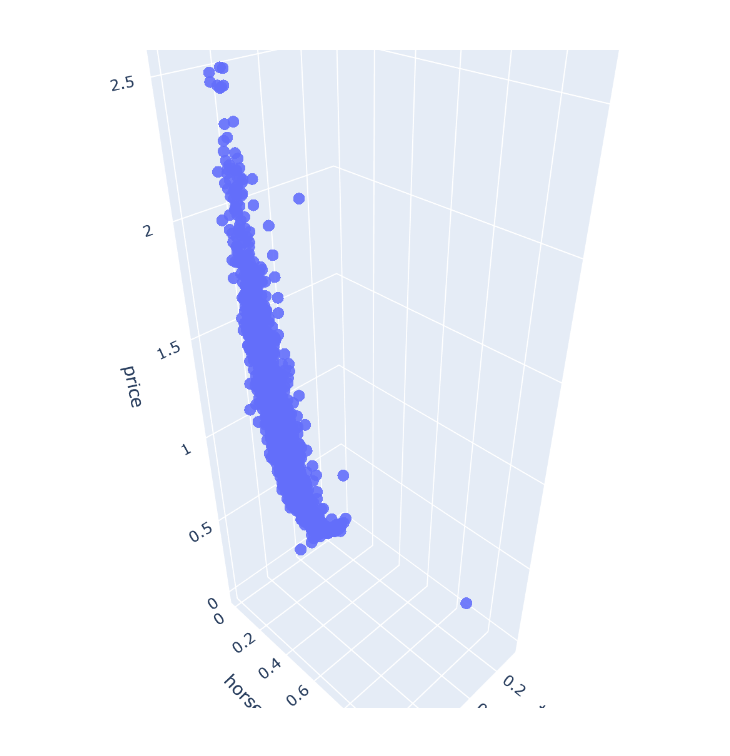
\includegraphics{01.png}

    \begin{tcolorbox}[breakable, size=fbox, boxrule=1pt, pad at break*=1mm,colback=cellbackground, colframe=cellborder]
\prompt{In}{incolor}{355}{\boxspacing}
\begin{Verbatim}[commandchars=\\\{\}]
\PY{n}{train\PYZus{}df}\PY{o}{.}\PY{n}{head}\PY{p}{(}\PY{p}{)}
\end{Verbatim}
\end{tcolorbox}

            \begin{tcolorbox}[breakable, size=fbox, boxrule=.5pt, pad at break*=1mm, opacityfill=0]
\prompt{Out}{outcolor}{355}{\boxspacing}
\begin{Verbatim}[commandchars=\\\{\}]
   Sex  Length  Diameter  Height  Whole weight  Shucked weight  \textbackslash{}
Id
1    M   0.455     0.365   0.095        0.5140          0.2245
2    M   0.350     0.265   0.090        0.2255          0.0995
3    F   0.530     0.420   0.135        0.6770          0.2565
4    M   0.440     0.365   0.125        0.5160          0.2155
5    I   0.425     0.300   0.095        0.3515          0.1410

    Viscera weight  Shell weight  Rings
Id
1           0.1010         0.150     15
2           0.0485         0.070      7
3           0.1415         0.210      9
4           0.1140         0.155     10
5           0.0775         0.120      8
\end{Verbatim}
\end{tcolorbox}
        
    \begin{tcolorbox}[breakable, size=fbox, boxrule=1pt, pad at break*=1mm,colback=cellbackground, colframe=cellborder]
\prompt{In}{incolor}{356}{\boxspacing}
\begin{Verbatim}[commandchars=\\\{\}]
\PY{n}{test\PYZus{}df}\PY{o}{.}\PY{n}{head}\PY{p}{(}\PY{p}{)}
\end{Verbatim}
\end{tcolorbox}

            \begin{tcolorbox}[breakable, size=fbox, boxrule=.5pt, pad at break*=1mm, opacityfill=0]
\prompt{Out}{outcolor}{356}{\boxspacing}
\begin{Verbatim}[commandchars=\\\{\}]
     Sex  Length  Diameter  Height  Whole weight  Shucked weight  \textbackslash{}
Id
3343   I   0.330     0.255   0.080        0.2050          0.0895
3344   F   0.550     0.440   0.150        0.8945          0.3145
3345   F   0.470     0.355   0.100        0.4755          0.1675
3346   M   0.450     0.320   0.100        0.3810          0.1705
3347   F   0.615     0.480   0.165        1.1615          0.5130

      Viscera weight  Shell weight
Id
3343          0.0395         0.055
3344          0.1510         0.320
3345          0.0805         0.185
3346          0.0750         0.115
3347          0.3010         0.305
\end{Verbatim}
\end{tcolorbox}
        
    \begin{tcolorbox}[breakable, size=fbox, boxrule=1pt, pad at break*=1mm,colback=cellbackground, colframe=cellborder]
\prompt{In}{incolor}{357}{\boxspacing}
\begin{Verbatim}[commandchars=\\\{\}]
\PY{c+c1}{\PYZsh{}将训练目标单独拿出}
\PY{n}{y\PYZus{}train} \PY{o}{=} \PY{n}{np}\PY{o}{.}\PY{n}{log1p}\PY{p}{(}\PY{n}{train\PYZus{}df}\PY{o}{.}\PY{n}{pop}\PY{p}{(}\PY{l+s+s2}{\PYZdq{}}\PY{l+s+s2}{Rings}\PY{l+s+s2}{\PYZdq{}}\PY{p}{)}\PY{p}{)}
\PY{n}{all\PYZus{}df} \PY{o}{=} \PY{n}{pd}\PY{o}{.}\PY{n}{concat}\PY{p}{(}\PY{p}{(}\PY{n}{train\PYZus{}df}\PY{p}{,} \PY{n}{test\PYZus{}df}\PY{p}{)}\PY{p}{,} \PY{n}{axis}\PY{o}{=}\PY{l+m+mi}{0}\PY{p}{)}
\PY{n}{all\PYZus{}df}\PY{o}{.}\PY{n}{shape}
\end{Verbatim}
\end{tcolorbox}

            \begin{tcolorbox}[breakable, size=fbox, boxrule=.5pt, pad at break*=1mm, opacityfill=0]
\prompt{Out}{outcolor}{357}{\boxspacing}
\begin{Verbatim}[commandchars=\\\{\}]
(4080, 8)
\end{Verbatim}
\end{tcolorbox}
        
    \begin{tcolorbox}[breakable, size=fbox, boxrule=1pt, pad at break*=1mm,colback=cellbackground, colframe=cellborder]
\prompt{In}{incolor}{358}{\boxspacing}
\begin{Verbatim}[commandchars=\\\{\}]
\PY{c+c1}{\PYZsh{}Sex被分成了3个column,每一个代表一个类。是就是1,不是就是0。}
\PY{n}{pd}\PY{o}{.}\PY{n}{get\PYZus{}dummies}\PY{p}{(}\PY{n}{all\PYZus{}df}\PY{p}{[}\PY{l+s+s1}{\PYZsq{}}\PY{l+s+s1}{Sex}\PY{l+s+s1}{\PYZsq{}}\PY{p}{]}\PY{p}{,} \PY{n}{prefix}\PY{o}{=}\PY{l+s+s1}{\PYZsq{}}\PY{l+s+s1}{Sex}\PY{l+s+s1}{\PYZsq{}}\PY{p}{)}\PY{o}{.}\PY{n}{head}\PY{p}{(}\PY{p}{)}
\end{Verbatim}
\end{tcolorbox}

            \begin{tcolorbox}[breakable, size=fbox, boxrule=.5pt, pad at break*=1mm, opacityfill=0]
\prompt{Out}{outcolor}{358}{\boxspacing}
\begin{Verbatim}[commandchars=\\\{\}]
    Sex\_F  Sex\_I  Sex\_M
Id
1       0      0      1
2       0      0      1
3       1      0      0
4       0      0      1
5       0      1      0
\end{Verbatim}
\end{tcolorbox}
        
    \begin{tcolorbox}[breakable, size=fbox, boxrule=1pt, pad at break*=1mm,colback=cellbackground, colframe=cellborder]
\prompt{In}{incolor}{359}{\boxspacing}
\begin{Verbatim}[commandchars=\\\{\}]
\PY{n}{all\PYZus{}dummy\PYZus{}df} \PY{o}{=} \PY{n}{pd}\PY{o}{.}\PY{n}{get\PYZus{}dummies}\PY{p}{(}\PY{n}{all\PYZus{}df}\PY{p}{)}
\PY{n}{all\PYZus{}dummy\PYZus{}df}\PY{o}{.}\PY{n}{head}\PY{p}{(}\PY{p}{)}
\end{Verbatim}
\end{tcolorbox}

            \begin{tcolorbox}[breakable, size=fbox, boxrule=.5pt, pad at break*=1mm, opacityfill=0]
\prompt{Out}{outcolor}{359}{\boxspacing}
\begin{Verbatim}[commandchars=\\\{\}]
    Length  Diameter  Height  Whole weight  Shucked weight  Viscera weight  \textbackslash{}
Id
1    0.455     0.365   0.095        0.5140          0.2245          0.1010
2    0.350     0.265   0.090        0.2255          0.0995          0.0485
3    0.530     0.420   0.135        0.6770          0.2565          0.1415
4    0.440     0.365   0.125        0.5160          0.2155          0.1140
5    0.425     0.300   0.095        0.3515          0.1410          0.0775

    Shell weight  Sex\_F  Sex\_I  Sex\_M
Id
1          0.150      0      0      1
2          0.070      0      0      1
3          0.210      1      0      0
4          0.155      0      0      1
5          0.120      0      1      0
\end{Verbatim}
\end{tcolorbox}
        
    \begin{tcolorbox}[breakable, size=fbox, boxrule=1pt, pad at break*=1mm,colback=cellbackground, colframe=cellborder]
\prompt{In}{incolor}{360}{\boxspacing}
\begin{Verbatim}[commandchars=\\\{\}]
\PY{n}{all\PYZus{}dummy\PYZus{}df}\PY{o}{.}\PY{n}{isnull}\PY{p}{(}\PY{p}{)}\PY{o}{.}\PY{n}{sum}\PY{p}{(}\PY{p}{)}\PY{o}{.}\PY{n}{sort\PYZus{}values}\PY{p}{(}\PY{n}{ascending}\PY{o}{=}\PY{k+kc}{False}\PY{p}{)}\PY{o}{.}\PY{n}{head}\PY{p}{(}\PY{l+m+mi}{10}\PY{p}{)}
\end{Verbatim}
\end{tcolorbox}

            \begin{tcolorbox}[breakable, size=fbox, boxrule=.5pt, pad at break*=1mm, opacityfill=0]
\prompt{Out}{outcolor}{360}{\boxspacing}
\begin{Verbatim}[commandchars=\\\{\}]
Sex\_M             0
Sex\_I             0
Sex\_F             0
Shell weight      0
Viscera weight    0
Shucked weight    0
Whole weight      0
Height            0
Diameter          0
Length            0
dtype: int64
\end{Verbatim}
\end{tcolorbox}
        
    \begin{tcolorbox}[breakable, size=fbox, boxrule=1pt, pad at break*=1mm,colback=cellbackground, colframe=cellborder]
\prompt{In}{incolor}{361}{\boxspacing}
\begin{Verbatim}[commandchars=\\\{\}]
\PY{n}{all\PYZus{}dummy\PYZus{}df}\PY{o}{.}\PY{n}{describe}\PY{p}{(}\PY{p}{)}
\end{Verbatim}
\end{tcolorbox}

            \begin{tcolorbox}[breakable, size=fbox, boxrule=.5pt, pad at break*=1mm, opacityfill=0]
\prompt{Out}{outcolor}{361}{\boxspacing}
\begin{Verbatim}[commandchars=\\\{\}]
            Length     Diameter       Height  Whole weight  Shucked weight  \textbackslash{}
count  4080.000000  4080.000000  4080.000000   4080.000000     4080.000000
mean      0.523960     0.407908     0.139507      0.828630        0.359151
std       0.119964     0.099141     0.041883      0.490842        0.222106
min       0.075000     0.055000     0.000000      0.002000        0.001000
25\%       0.450000     0.350000     0.115000      0.441375        0.186000
50\%       0.545000     0.425000     0.140000      0.799750        0.336000
75\%       0.615000     0.480000     0.165000      1.151500        0.500625
max       0.815000     0.650000     1.130000      2.825500        1.488000

       Viscera weight  Shell weight        Sex\_F        Sex\_I        Sex\_M
count     4080.000000   4080.000000  4080.000000  4080.000000  4080.000000
mean         0.180484      0.238873     0.313480     0.321569     0.364951
std          0.109632      0.139466     0.463965     0.467136     0.481475
min          0.000500      0.001500     0.000000     0.000000     0.000000
25\%          0.093000      0.130000     0.000000     0.000000     0.000000
50\%          0.170500      0.232750     0.000000     0.000000     0.000000
75\%          0.252500      0.328625     1.000000     1.000000     1.000000
max          0.760000      1.005000     1.000000     1.000000     1.000000
\end{Verbatim}
\end{tcolorbox}
        
    \begin{tcolorbox}[breakable, size=fbox, boxrule=1pt, pad at break*=1mm,colback=cellbackground, colframe=cellborder]
\prompt{In}{incolor}{362}{\boxspacing}
\begin{Verbatim}[commandchars=\\\{\}]
\PY{k+kn}{import} \PY{n+nn}{seaborn} \PY{k}{as} \PY{n+nn}{sns}
\PY{k+kn}{import} \PY{n+nn}{matplotlib}\PY{n+nn}{.}\PY{n+nn}{style} \PY{k}{as} \PY{n+nn}{style}
\PY{n}{sns}\PY{o}{.}\PY{n}{heatmap}\PY{p}{(}\PY{n}{all\PYZus{}dummy\PYZus{}df}\PY{o}{.}\PY{n}{corr}\PY{p}{(}\PY{p}{)}\PY{p}{,}\PY{n}{cmap}\PY{o}{=}\PY{l+s+s1}{\PYZsq{}}\PY{l+s+s1}{YlGnBu}\PY{l+s+s1}{\PYZsq{}}\PY{p}{)}
\end{Verbatim}
\end{tcolorbox}

            \begin{tcolorbox}[breakable, size=fbox, boxrule=.5pt, pad at break*=1mm, opacityfill=0]
\prompt{Out}{outcolor}{362}{\boxspacing}
\begin{Verbatim}[commandchars=\\\{\}]
<matplotlib.axes.\_subplots.AxesSubplot at 0x1bd8cee0308>
\end{Verbatim}
\end{tcolorbox}
        
    \begin{center}
    \adjustimage{max size={0.9\linewidth}{0.9\paperheight}}{output_171_1.png}
    \end{center}
    { \hspace*{\fill} \\}
    
    \begin{tcolorbox}[breakable, size=fbox, boxrule=1pt, pad at break*=1mm,colback=cellbackground, colframe=cellborder]
\prompt{In}{incolor}{363}{\boxspacing}
\begin{Verbatim}[commandchars=\\\{\}]
\PY{n}{dummy\PYZus{}train\PYZus{}df} \PY{o}{=} \PY{n}{all\PYZus{}dummy\PYZus{}df}\PY{o}{.}\PY{n}{loc}\PY{p}{[}\PY{n}{train\PYZus{}df}\PY{o}{.}\PY{n}{index}\PY{p}{]}
\PY{n}{dummy\PYZus{}test\PYZus{}df} \PY{o}{=} \PY{n}{all\PYZus{}dummy\PYZus{}df}\PY{o}{.}\PY{n}{loc}\PY{p}{[}\PY{n}{test\PYZus{}df}\PY{o}{.}\PY{n}{index}\PY{p}{]}
\end{Verbatim}
\end{tcolorbox}

    \begin{tcolorbox}[breakable, size=fbox, boxrule=1pt, pad at break*=1mm,colback=cellbackground, colframe=cellborder]
\prompt{In}{incolor}{364}{\boxspacing}
\begin{Verbatim}[commandchars=\\\{\}]
\PY{n}{X\PYZus{}train} \PY{o}{=} \PY{n}{dummy\PYZus{}train\PYZus{}df}\PY{o}{.}\PY{n}{values}
\PY{c+c1}{\PYZsh{} X\PYZus{}test = dummy\PYZus{}test\PYZus{}df.values}
\PY{n}{X\PYZus{}train}\PY{p}{,}\PY{n}{X\PYZus{}test}\PY{p}{,}\PY{n}{Y\PYZus{}train}\PY{p}{,}\PY{n}{Y\PYZus{}test} \PY{o}{=} \PY{n}{train\PYZus{}test\PYZus{}split}\PY{p}{(}\PY{n}{dummy\PYZus{}train\PYZus{}df}\PY{o}{.}\PY{n}{values}\PY{p}{,}\PY{n}{y\PYZus{}train}\PY{p}{,}\PY{n}{train\PYZus{}size}\PY{o}{=}\PY{o}{.}\PY{l+m+mi}{8}\PY{p}{)}
\PY{n+nb}{print}\PY{p}{(}\PY{l+s+s2}{\PYZdq{}}\PY{l+s+s2}{原始数据特征:}\PY{l+s+s2}{\PYZdq{}}\PY{p}{,}\PY{n}{dummy\PYZus{}train\PYZus{}df}\PY{o}{.}\PY{n}{shape}\PY{p}{,}      \PY{l+s+s2}{\PYZdq{}}\PY{l+s+s2}{,训练数据特征:}\PY{l+s+s2}{\PYZdq{}}\PY{p}{,}\PY{n}{X\PYZus{}train}\PY{o}{.}\PY{n}{shape}\PY{p}{,}      \PY{l+s+s2}{\PYZdq{}}\PY{l+s+s2}{,测试数据特征:}\PY{l+s+s2}{\PYZdq{}}\PY{p}{,}\PY{n}{X\PYZus{}test}\PY{o}{.}\PY{n}{shape}\PY{p}{)} 
\PY{n+nb}{print}\PY{p}{(}\PY{l+s+s2}{\PYZdq{}}\PY{l+s+s2}{原始数据标签:}\PY{l+s+s2}{\PYZdq{}}\PY{p}{,}\PY{n}{y\PYZus{}train}\PY{o}{.}\PY{n}{shape}\PY{p}{,}      \PY{l+s+s2}{\PYZdq{}}\PY{l+s+s2}{,训练数据标签:}\PY{l+s+s2}{\PYZdq{}}\PY{p}{,}\PY{n}{Y\PYZus{}train}\PY{o}{.}\PY{n}{shape}\PY{p}{,}      \PY{l+s+s2}{\PYZdq{}}\PY{l+s+s2}{,测试数据标签:}\PY{l+s+s2}{\PYZdq{}}\PY{p}{,}\PY{n}{Y\PYZus{}test}\PY{o}{.}\PY{n}{shape}\PY{p}{)} 
\end{Verbatim}
\end{tcolorbox}

    \begin{Verbatim}[commandchars=\\\{\}]
原始数据特征: (3342, 10) ,训练数据特征: (2673, 10) ,测试数据特征: (669, 10)
原始数据标签: (3342,) ,训练数据标签: (2673,) ,测试数据标签: (669,)
    \end{Verbatim}

    \begin{tcolorbox}[breakable, size=fbox, boxrule=1pt, pad at break*=1mm,colback=cellbackground, colframe=cellborder]
\prompt{In}{incolor}{368}{\boxspacing}
\begin{Verbatim}[commandchars=\\\{\}]
\PY{n}{model}\PY{o}{.}\PY{n}{fit}\PY{p}{(}\PY{n}{X\PYZus{}train}\PY{p}{,}\PY{n}{Y\PYZus{}train}\PY{p}{)}
\PY{n}{Y\PYZus{}pre} \PY{o}{=} \PY{n}{model}\PY{o}{.}\PY{n}{predict}\PY{p}{(}\PY{n}{X\PYZus{}test}\PY{p}{)}
\end{Verbatim}
\end{tcolorbox}

    \begin{tcolorbox}[breakable, size=fbox, boxrule=1pt, pad at break*=1mm,colback=cellbackground, colframe=cellborder]
\prompt{In}{incolor}{369}{\boxspacing}
\begin{Verbatim}[commandchars=\\\{\}]
\PY{n}{a}  \PY{o}{=} \PY{n}{model}\PY{o}{.}\PY{n}{intercept\PYZus{}}
\PY{n}{b} \PY{o}{=} \PY{n}{model}\PY{o}{.}\PY{n}{coef\PYZus{}}
\PY{n+nb}{print}\PY{p}{(}\PY{l+s+s2}{\PYZdq{}}\PY{l+s+s2}{最佳拟合线:截距}\PY{l+s+s2}{\PYZdq{}}\PY{p}{,}\PY{n}{a}\PY{p}{,}\PY{l+s+s2}{\PYZdq{}}\PY{l+s+s2}{,回归系数:}\PY{l+s+s2}{\PYZdq{}}\PY{p}{,}\PY{n}{b}\PY{p}{)}
\end{Verbatim}
\end{tcolorbox}

    \begin{Verbatim}[commandchars=\\\{\}]
最佳拟合线:截距 624148452518.2838 ,回归系数: [ 3.75423803e-01  1.39775905e+00
8.90195444e-01  5.46505689e-01
 -1.50963697e+00 -7.08881891e-01  5.58664600e-01 -6.24148453e+11
 -6.24148453e+11 -6.24148453e+11]
    \end{Verbatim}

    \begin{tcolorbox}[breakable, size=fbox, boxrule=1pt, pad at break*=1mm,colback=cellbackground, colframe=cellborder]
\prompt{In}{incolor}{371}{\boxspacing}
\begin{Verbatim}[commandchars=\\\{\}]
\PY{n}{plt}\PY{o}{.}\PY{n}{scatter}\PY{p}{(}\PY{n}{Y\PYZus{}pre}\PY{p}{,}\PY{n}{Y\PYZus{}test}\PY{p}{,}\PY{n}{marker}\PY{o}{=}\PY{l+s+s1}{\PYZsq{}}\PY{l+s+s1}{o}\PY{l+s+s1}{\PYZsq{}}\PY{p}{)}
\PY{n}{plt}\PY{o}{.}\PY{n}{scatter}\PY{p}{(}\PY{n}{Y\PYZus{}test}\PY{p}{,}\PY{n}{Y\PYZus{}test}\PY{p}{)}
\PY{n}{plt}\PY{o}{.}\PY{n}{show}\PY{p}{(}\PY{p}{)}
\end{Verbatim}
\end{tcolorbox}

    \begin{center}
    \adjustimage{max size={0.9\linewidth}{0.9\paperheight}}{output_176_0.png}
    \end{center}
    { \hspace*{\fill} \\}
    
    \begin{itemize}
\tightlist
\item
  问题:欠拟合
\item
  解决办法:局部加权回归(更复杂的模型)
\end{itemize}

    \hypertarget{ux4f5cux4e1aux6e05ux535556}{%
\section{作业清单(5/6)}\label{ux4f5cux4e1aux6e05ux535556}}

    \hypertarget{ux95eeux9898ux4e00-ux6570ux636eux6e05ux6d17}{%
\subsection{问题一
数据清洗}\label{ux95eeux9898ux4e00-ux6570ux636eux6e05ux6d17}}

    【1】
数据清洗是数据挖掘模型建立过程中很重要的一步吗一般,清洗的方法包括什么?

    数据清洗是数据挖掘模型建立过程中很重要的一步。\href{https://zhuanlan.zhihu.com/p/40775756}{数据清理方法}

    通过填写缺失的值,光滑噪声数据,识别或删除离群点,并解决不一致性来``清理''数据。如果用户认为数据是脏的,则他们可能不会相信这些数据上的挖掘结果。此外,脏数据可能使挖掘过程陷入混乱,导致不可靠的输出。

    \hypertarget{ux7f3aux5931ux503c}{%
\subsubsection{缺失值}\label{ux7f3aux5931ux503c}}

    \begin{itemize}
\tightlist
\item
  \textbf{忽略元组:}当缺少类标号时通常这样做(假定挖掘任务涉及分类)。除非元组有多个属性缺少值,否则该方法不是很有效。当每个属性缺失值的百分比变化很大时,它的性能特别差。采用忽略元组,你不能使用该元组的剩余属性值。这些数据可能对手头的任务是有用的。
\item
  \textbf{人工填写缺失值:}一般来说,该方法很费时,并且当数据集很大、确实很多值时,该方法可能行不通。
\item
  \textbf{使用一个全局常量填充缺失值:}将缺失的属性值用同一个常量(如
  ``Unknown'' 或 \(-\infty\))替换。如果缺失值都用 ``Unknown''
  替换,则挖掘程序可能误以为他们形成了一个有趣的概念,因为它们都具有相同的值------
  ``Unknown'' 。因此,尽管该方法简单,但并不十分可靠。
\item
  \textbf{使用属性的中心度量(如均值或中位数)填充缺失值:}均值等中心趋势度量,指示数据分布的``中间''值。对于正常的(对称的)数据分布而言,可以使用均值,而倾斜数据分布应该使用中位数。例如,收入的数据是对称的,并且平均收入为
  56,000 美元,则使用该值替换收入属性中的缺失值。
\item
  \textbf{使用与给定元组属同一类的所有样本的属性均值或中位数:}例如,将顾客按信用等级分类,则用具有相同信用风险的顾客的平均收入替换收入属性中的缺失值。如果给定类的数据分布是倾斜的,则中位数是更好的选择。
\item
  \textbf{使用最可能的值填充缺失值:}可以用回归、使用贝叶斯形式化方法的基于推理的工具或决策树归纳确定。例如,利用数据集中其他顾客的属性,可以构造一颗决策树,来预测收入的缺失值。
\end{itemize}

    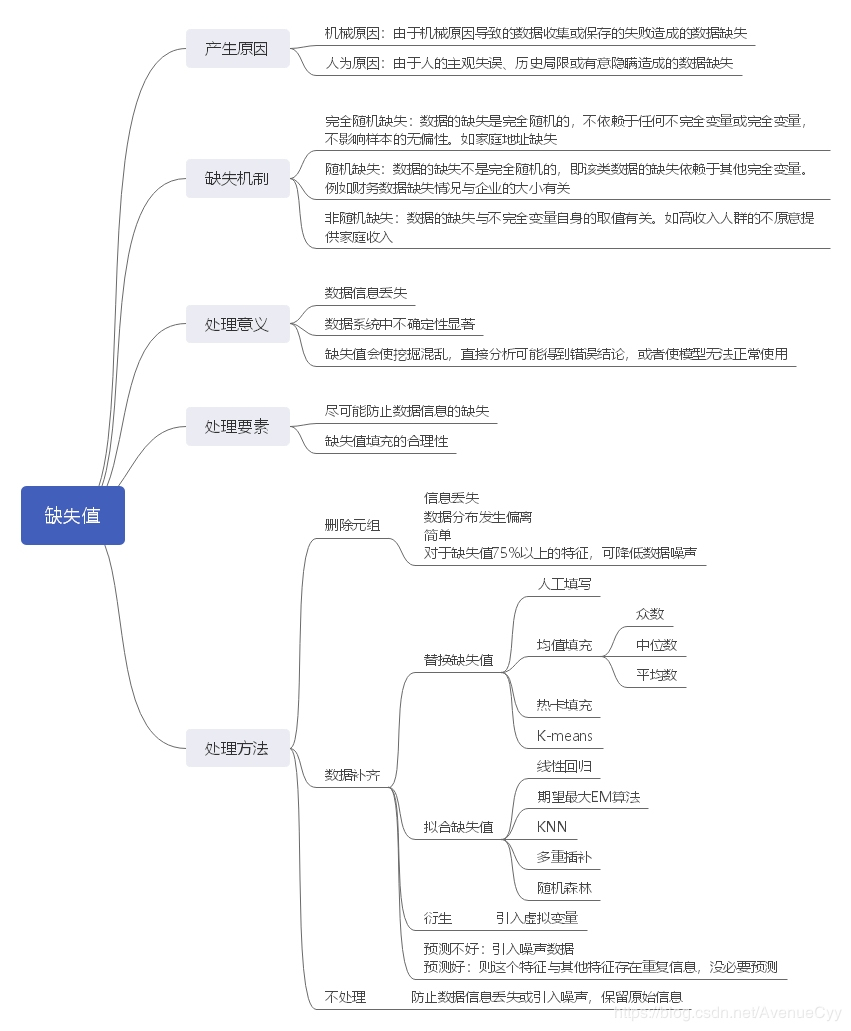
\includegraphics{02.jpg}

    \hypertarget{ux566aux58f0ux6570ux636e}{%
\subsubsection{噪声数据}\label{ux566aux58f0ux6570ux636e}}

    \textbf{噪声}是被测量的变量的随机误差或方差。

    数据光滑技术: -
\textbf{分箱:}通过考察数据的``近邻''(即周围的值)来光滑有序数据值。这些有序的值被分布到一些``桶''或箱中。由于分箱方法考察临近的值,因此它进行局部光滑。
- \textbf{回归:}可以用一个函数拟合数据来光滑数据。 -
\textbf{离群点分析:}可以通过如聚类来检测离群点。聚类将类似的值组织成群或``簇''。

    \hypertarget{ux95eeux9898ux4e8c-ux5220ux9664ux548cux586bux8865}{%
\subsection{问题二
删除和填补}\label{ux95eeux9898ux4e8c-ux5220ux9664ux548cux586bux8865}}

    【2】 对下图的数据采用删除和填补两种方法进行清洗。

    \begin{tcolorbox}[breakable, size=fbox, boxrule=1pt, pad at break*=1mm,colback=cellbackground, colframe=cellborder]
\prompt{In}{incolor}{ }{\boxspacing}
\begin{Verbatim}[commandchars=\\\{\}]
\PY{k+kn}{import} \PY{n+nn}{pandas} \PY{k}{as} \PY{n+nn}{pd} 
\end{Verbatim}
\end{tcolorbox}

    \begin{tcolorbox}[breakable, size=fbox, boxrule=1pt, pad at break*=1mm,colback=cellbackground, colframe=cellborder]
\prompt{In}{incolor}{377}{\boxspacing}
\begin{Verbatim}[commandchars=\\\{\}]
\PY{n}{data}\PY{o}{=}\PY{n}{pd}\PY{o}{.}\PY{n}{read\PYZus{}csv}\PY{p}{(}\PY{l+s+s2}{\PYZdq{}}\PY{l+s+s2}{homework\PYZus{}3.csv}\PY{l+s+s2}{\PYZdq{}}\PY{p}{)}
\PY{n}{data}\PY{o}{.}\PY{n}{head}\PY{p}{(}\PY{p}{)}
\end{Verbatim}
\end{tcolorbox}

            \begin{tcolorbox}[breakable, size=fbox, boxrule=.5pt, pad at break*=1mm, opacityfill=0]
\prompt{Out}{outcolor}{377}{\boxspacing}
\begin{Verbatim}[commandchars=\\\{\}]
   Sepal.Length  Sepal.Width  Pepal.Length  Pepal.Width Species
0           5.1          3.5           1.4          0.2  setosa
1           4.9          3.0           NaN          0.2  setosa
2           4.7          3.2           NaN          0.2  setosa
3           4.6          3.1           1.5          0.2  setosa
4           5.1          3.8           NaN          0.2  setosa
\end{Verbatim}
\end{tcolorbox}
        
    \begin{tcolorbox}[breakable, size=fbox, boxrule=1pt, pad at break*=1mm,colback=cellbackground, colframe=cellborder]
\prompt{In}{incolor}{378}{\boxspacing}
\begin{Verbatim}[commandchars=\\\{\}]
\PY{n}{data}\PY{o}{.}\PY{n}{describe}\PY{p}{(}\PY{p}{)}
\end{Verbatim}
\end{tcolorbox}

            \begin{tcolorbox}[breakable, size=fbox, boxrule=.5pt, pad at break*=1mm, opacityfill=0]
\prompt{Out}{outcolor}{378}{\boxspacing}
\begin{Verbatim}[commandchars=\\\{\}]
       Sepal.Length  Sepal.Width  Pepal.Length  Pepal.Width
count     14.000000    14.000000      9.000000    15.000000
mean       5.500000     3.171429      3.177778     0.973333
std        0.775589     0.267261      2.090322     0.889194
min        4.600000     2.700000      1.400000     0.200000
25\%        4.925000     3.000000      1.400000     0.200000
50\%        5.200000     3.200000      1.500000     0.200000
75\%        6.200000     3.275000      5.100000     1.800000
max        7.000000     3.800000      6.000000     2.500000
\end{Verbatim}
\end{tcolorbox}
        
    \begin{tcolorbox}[breakable, size=fbox, boxrule=1pt, pad at break*=1mm,colback=cellbackground, colframe=cellborder]
\prompt{In}{incolor}{379}{\boxspacing}
\begin{Verbatim}[commandchars=\\\{\}]
\PY{n}{data}\PY{o}{.}\PY{n}{isnull}\PY{p}{(}\PY{p}{)}\PY{o}{.}\PY{n}{sum}\PY{p}{(}\PY{p}{)}\PY{o}{.}\PY{n}{sort\PYZus{}values}\PY{p}{(}\PY{n}{ascending}\PY{o}{=}\PY{k+kc}{False}\PY{p}{)}
\end{Verbatim}
\end{tcolorbox}

            \begin{tcolorbox}[breakable, size=fbox, boxrule=.5pt, pad at break*=1mm, opacityfill=0]
\prompt{Out}{outcolor}{379}{\boxspacing}
\begin{Verbatim}[commandchars=\\\{\}]
Pepal.Length    6
Sepal.Width     1
Sepal.Length    1
Species         0
Pepal.Width     0
dtype: int64
\end{Verbatim}
\end{tcolorbox}
        
    \hypertarget{ux5220ux9664}{%
\subsubsection{删除}\label{ux5220ux9664}}

    \begin{tcolorbox}[breakable, size=fbox, boxrule=1pt, pad at break*=1mm,colback=cellbackground, colframe=cellborder]
\prompt{In}{incolor}{380}{\boxspacing}
\begin{Verbatim}[commandchars=\\\{\}]
\PY{c+c1}{\PYZsh{} 删除 nan 所在行}
\PY{n}{data1}\PY{o}{=}\PY{n}{data}\PY{o}{.}\PY{n}{dropna}\PY{p}{(}\PY{p}{)}
\PY{n}{data1}
\end{Verbatim}
\end{tcolorbox}

            \begin{tcolorbox}[breakable, size=fbox, boxrule=.5pt, pad at break*=1mm, opacityfill=0]
\prompt{Out}{outcolor}{380}{\boxspacing}
\begin{Verbatim}[commandchars=\\\{\}]
    Sepal.Length  Sepal.Width  Pepal.Length  Pepal.Width     Species
0            5.1          3.5           1.4          0.2      setosa
3            4.6          3.1           1.5          0.2      setosa
5            4.6          3.2           1.4          0.2      setosa
7            5.0          3.3           1.4          0.2      setosa
8            7.0          3.2           4.7          1.4  versicolor
10           6.3          3.3           6.0          2.5   virginica
11           5.8          2.7           5.1          1.9   virginica
13           6.3          2.9           5.6          1.8   virginica
\end{Verbatim}
\end{tcolorbox}
        
    \begin{tcolorbox}[breakable, size=fbox, boxrule=1pt, pad at break*=1mm,colback=cellbackground, colframe=cellborder]
\prompt{In}{incolor}{381}{\boxspacing}
\begin{Verbatim}[commandchars=\\\{\}]
\PY{c+c1}{\PYZsh{} 删除 nan 所在列}
\PY{n}{data2}\PY{o}{=}\PY{n}{data}\PY{o}{.}\PY{n}{dropna}\PY{p}{(}\PY{n}{axis}\PY{o}{=}\PY{l+m+mi}{1}\PY{p}{)}
\PY{n}{data2}
\end{Verbatim}
\end{tcolorbox}

            \begin{tcolorbox}[breakable, size=fbox, boxrule=.5pt, pad at break*=1mm, opacityfill=0]
\prompt{Out}{outcolor}{381}{\boxspacing}
\begin{Verbatim}[commandchars=\\\{\}]
    Pepal.Width     Species
0           0.2      setosa
1           0.2      setosa
2           0.2      setosa
3           0.2      setosa
4           0.2      setosa
5           0.2      setosa
6           0.2      setosa
7           0.2      setosa
8           1.4  versicolor
9           1.5  versicolor
10          2.5   virginica
11          1.9   virginica
12          2.1   virginica
13          1.8   virginica
14          1.8   virginica
\end{Verbatim}
\end{tcolorbox}
        
    \hypertarget{ux586bux8865}{%
\subsubsection{填补}\label{ux586bux8865}}

    \begin{tcolorbox}[breakable, size=fbox, boxrule=1pt, pad at break*=1mm,colback=cellbackground, colframe=cellborder]
\prompt{In}{incolor}{382}{\boxspacing}
\begin{Verbatim}[commandchars=\\\{\}]
\PY{c+c1}{\PYZsh{} 用0填充缺省值}
\PY{n}{data3}\PY{o}{=}\PY{n}{data}\PY{o}{.}\PY{n}{fillna}\PY{p}{(}\PY{l+m+mi}{0}\PY{p}{)}
\PY{n}{data3}
\end{Verbatim}
\end{tcolorbox}

            \begin{tcolorbox}[breakable, size=fbox, boxrule=.5pt, pad at break*=1mm, opacityfill=0]
\prompt{Out}{outcolor}{382}{\boxspacing}
\begin{Verbatim}[commandchars=\\\{\}]
    Sepal.Length  Sepal.Width  Pepal.Length  Pepal.Width     Species
0            5.1          3.5           1.4          0.2      setosa
1            4.9          3.0           0.0          0.2      setosa
2            4.7          3.2           0.0          0.2      setosa
3            4.6          3.1           1.5          0.2      setosa
4            5.1          3.8           0.0          0.2      setosa
5            4.6          3.2           1.4          0.2      setosa
6            5.3          0.0           1.5          0.2      setosa
7            5.0          3.3           1.4          0.2      setosa
8            7.0          3.2           4.7          1.4  versicolor
9            6.4          3.2           0.0          1.5  versicolor
10           6.3          3.3           6.0          2.5   virginica
11           5.8          2.7           5.1          1.9   virginica
12           0.0          3.0           0.0          2.1   virginica
13           6.3          2.9           5.6          1.8   virginica
14           5.9          3.0           0.0          1.8   virginica
\end{Verbatim}
\end{tcolorbox}
        
    \begin{tcolorbox}[breakable, size=fbox, boxrule=1pt, pad at break*=1mm,colback=cellbackground, colframe=cellborder]
\prompt{In}{incolor}{383}{\boxspacing}
\begin{Verbatim}[commandchars=\\\{\}]
\PY{c+c1}{\PYZsh{} 用上一个数据填充缺省值}
\PY{n}{data4}\PY{o}{=}\PY{n}{data}\PY{o}{.}\PY{n}{fillna}\PY{p}{(}\PY{n}{method}\PY{o}{=}\PY{l+s+s2}{\PYZdq{}}\PY{l+s+s2}{pad}\PY{l+s+s2}{\PYZdq{}}\PY{p}{)}
\PY{n}{data4}
\end{Verbatim}
\end{tcolorbox}

            \begin{tcolorbox}[breakable, size=fbox, boxrule=.5pt, pad at break*=1mm, opacityfill=0]
\prompt{Out}{outcolor}{383}{\boxspacing}
\begin{Verbatim}[commandchars=\\\{\}]
    Sepal.Length  Sepal.Width  Pepal.Length  Pepal.Width     Species
0            5.1          3.5           1.4          0.2      setosa
1            4.9          3.0           1.4          0.2      setosa
2            4.7          3.2           1.4          0.2      setosa
3            4.6          3.1           1.5          0.2      setosa
4            5.1          3.8           1.5          0.2      setosa
5            4.6          3.2           1.4          0.2      setosa
6            5.3          3.2           1.5          0.2      setosa
7            5.0          3.3           1.4          0.2      setosa
8            7.0          3.2           4.7          1.4  versicolor
9            6.4          3.2           4.7          1.5  versicolor
10           6.3          3.3           6.0          2.5   virginica
11           5.8          2.7           5.1          1.9   virginica
12           5.8          3.0           5.1          2.1   virginica
13           6.3          2.9           5.6          1.8   virginica
14           5.9          3.0           5.6          1.8   virginica
\end{Verbatim}
\end{tcolorbox}
        
    \begin{tcolorbox}[breakable, size=fbox, boxrule=1pt, pad at break*=1mm,colback=cellbackground, colframe=cellborder]
\prompt{In}{incolor}{384}{\boxspacing}
\begin{Verbatim}[commandchars=\\\{\}]
\PY{c+c1}{\PYZsh{} 用平均值填充缺省值}
\PY{n}{data5}\PY{o}{=}\PY{n}{data}\PY{o}{.}\PY{n}{fillna}\PY{p}{(}\PY{n}{data}\PY{o}{.}\PY{n}{mean}\PY{p}{(}\PY{p}{)}\PY{p}{)}
\PY{n}{data5}
\end{Verbatim}
\end{tcolorbox}

            \begin{tcolorbox}[breakable, size=fbox, boxrule=.5pt, pad at break*=1mm, opacityfill=0]
\prompt{Out}{outcolor}{384}{\boxspacing}
\begin{Verbatim}[commandchars=\\\{\}]
    Sepal.Length  Sepal.Width  Pepal.Length  Pepal.Width     Species
0            5.1     3.500000      1.400000          0.2      setosa
1            4.9     3.000000      3.177778          0.2      setosa
2            4.7     3.200000      3.177778          0.2      setosa
3            4.6     3.100000      1.500000          0.2      setosa
4            5.1     3.800000      3.177778          0.2      setosa
5            4.6     3.200000      1.400000          0.2      setosa
6            5.3     3.171429      1.500000          0.2      setosa
7            5.0     3.300000      1.400000          0.2      setosa
8            7.0     3.200000      4.700000          1.4  versicolor
9            6.4     3.200000      3.177778          1.5  versicolor
10           6.3     3.300000      6.000000          2.5   virginica
11           5.8     2.700000      5.100000          1.9   virginica
12           5.5     3.000000      3.177778          2.1   virginica
13           6.3     2.900000      5.600000          1.8   virginica
14           5.9     3.000000      3.177778          1.8   virginica
\end{Verbatim}
\end{tcolorbox}
        
    \hypertarget{ux95eeux9898ux4e09-ux56deux5f52ux65b9ux6cd5ux586bux8865}{%
\subsection{问题三
回归方法填补}\label{ux95eeux9898ux4e09-ux56deux5f52ux65b9ux6cd5ux586bux8865}}

    【3】 对【2】题数据采用回归方法填补。

    \hypertarget{ux80ccux666fux63cfux8ff0}{%
\subsection{背景描述:}\label{ux80ccux666fux63cfux8ff0}}

数据清洗过程中经常会遇到异常值和缺失值等问题,有时候,会把异常值看作缺失值来处理。一般的缺失值处理方法包括:删除、统计值充填(均值、中位数等)、回归方程预测充填等。
使用直接删除这种方法简单易行,但缺点是,在记录数据较少的情况下,会造成样本量的进一步减少,可能会改变响应变量的原有分布,造成分析结果不准确。因此,将异常值视为缺失值来处理的益处在于可以利用现有变量的信息进行建模挖掘,对异常值(缺失值)进行填补。

\hypertarget{ux5e94ux7528ux573aux666f}{%
\subsection{应用场景:}\label{ux5e94ux7528ux573aux666f}}

\textbf{回归方程充填法}是选择若干能预测缺失值的自变量,通过建立回归方程估算缺失值。

该方法能尽可能地利用原数据集中的信息,但也存在一些不足之处: -
虽然这是一个无偏估计,但会忽视随机误差,低估标准差和其他未知性质的测量值;
-
使用前,必须假设存在缺失值所在的变量与其他变量是存在线性关系的,但现实它们不一定存在这样的线性关系,这可以借助统计工具来辨析,但往往更需要建模人员的实践经验和业务知识来进行分析和判断。

\hypertarget{ux65b9ux6cd5ux6b65ux9aa4}{%
\subsection{方法步骤:}\label{ux65b9ux6cd5ux6b65ux9aa4}}

\begin{itemize}
\item
  确定充填缺失值的变量(特征列)
\item
  拆分原始数据集: 根据需要充填缺失值的变量,把原始数据集拆分为2个子集

  \begin{itemize}
  \tightlist
  \item
    不含有缺失值:dataset\_train
  \item
    只含有缺失值:dataset\_pred
  \end{itemize}
\item
  辨析并检验相关变量的相关性:
  经验分析判定与充填缺失值的变量相关的属性列有哪些,应用统计分析工具,在dataset\_train数据集上查看验证所选择的属性列之间的相关性。
\item
  建模并预测:
  使用dataset\_train数据集建立线性回归模型,并应用建好的模型对dataset\_pred数据集中的缺失变量进行预测估计
\item
  合并还原数据集:
  将两个子集合并还原为一个数据集,为后续建模准备好数据。
\end{itemize}

    \begin{tcolorbox}[breakable, size=fbox, boxrule=1pt, pad at break*=1mm,colback=cellbackground, colframe=cellborder]
\prompt{In}{incolor}{386}{\boxspacing}
\begin{Verbatim}[commandchars=\\\{\}]
\PY{n}{data}\PY{o}{.}\PY{n}{info}\PY{p}{(}\PY{p}{)}
\end{Verbatim}
\end{tcolorbox}

    \begin{Verbatim}[commandchars=\\\{\}]
<class 'pandas.core.frame.DataFrame'>
RangeIndex: 15 entries, 0 to 14
Data columns (total 5 columns):
Sepal.Length    14 non-null float64
Sepal.Width     14 non-null float64
Pepal.Length    9 non-null float64
Pepal.Width     15 non-null float64
Species         15 non-null object
dtypes: float64(4), object(1)
memory usage: 728.0+ bytes
    \end{Verbatim}

    \begin{tcolorbox}[breakable, size=fbox, boxrule=1pt, pad at break*=1mm,colback=cellbackground, colframe=cellborder]
\prompt{In}{incolor}{387}{\boxspacing}
\begin{Verbatim}[commandchars=\\\{\}]
\PY{n}{data}\PY{o}{.}\PY{n}{isnull}\PY{p}{(}\PY{p}{)}\PY{o}{.}\PY{n}{sum}\PY{p}{(}\PY{p}{)}\PY{o}{.}\PY{n}{sort\PYZus{}values}\PY{p}{(}\PY{n}{ascending}\PY{o}{=}\PY{k+kc}{False}\PY{p}{)}
\end{Verbatim}
\end{tcolorbox}

            \begin{tcolorbox}[breakable, size=fbox, boxrule=.5pt, pad at break*=1mm, opacityfill=0]
\prompt{Out}{outcolor}{387}{\boxspacing}
\begin{Verbatim}[commandchars=\\\{\}]
Pepal.Length    6
Sepal.Width     1
Sepal.Length    1
Species         0
Pepal.Width     0
dtype: int64
\end{Verbatim}
\end{tcolorbox}
        
    \begin{tcolorbox}[breakable, size=fbox, boxrule=1pt, pad at break*=1mm,colback=cellbackground, colframe=cellborder]
\prompt{In}{incolor}{388}{\boxspacing}
\begin{Verbatim}[commandchars=\\\{\}]
\PY{c+c1}{\PYZsh{} 观察变量之间的相关性}
\PY{n}{dataset\PYZus{}train}\PY{o}{=}\PY{n}{data}\PY{o}{.}\PY{n}{dropna}\PY{p}{(}\PY{p}{)}
\PY{n}{dataset\PYZus{}train}
\end{Verbatim}
\end{tcolorbox}

            \begin{tcolorbox}[breakable, size=fbox, boxrule=.5pt, pad at break*=1mm, opacityfill=0]
\prompt{Out}{outcolor}{388}{\boxspacing}
\begin{Verbatim}[commandchars=\\\{\}]
    Sepal.Length  Sepal.Width  Pepal.Length  Pepal.Width     Species
0            5.1          3.5           1.4          0.2      setosa
3            4.6          3.1           1.5          0.2      setosa
5            4.6          3.2           1.4          0.2      setosa
7            5.0          3.3           1.4          0.2      setosa
8            7.0          3.2           4.7          1.4  versicolor
10           6.3          3.3           6.0          2.5   virginica
11           5.8          2.7           5.1          1.9   virginica
13           6.3          2.9           5.6          1.8   virginica
\end{Verbatim}
\end{tcolorbox}
        
    \begin{tcolorbox}[breakable, size=fbox, boxrule=1pt, pad at break*=1mm,colback=cellbackground, colframe=cellborder]
\prompt{In}{incolor}{389}{\boxspacing}
\begin{Verbatim}[commandchars=\\\{\}]
\PY{k+kn}{import} \PY{n+nn}{seaborn} \PY{k}{as} \PY{n+nn}{sns}
\PY{k+kn}{import} \PY{n+nn}{matplotlib}\PY{n+nn}{.}\PY{n+nn}{style} \PY{k}{as} \PY{n+nn}{style}
\PY{c+c1}{\PYZsh{} style.use(\PYZdq{}fivethirtyeight\PYZdq{})}
\PY{n}{sns}\PY{o}{.}\PY{n}{heatmap}\PY{p}{(}\PY{n}{dataset\PYZus{}train}\PY{o}{.}\PY{n}{corr}\PY{p}{(}\PY{p}{)}\PY{p}{,}\PY{n}{cmap}\PY{o}{=}\PY{l+s+s1}{\PYZsq{}}\PY{l+s+s1}{YlGnBu}\PY{l+s+s1}{\PYZsq{}}\PY{p}{)}
\end{Verbatim}
\end{tcolorbox}

            \begin{tcolorbox}[breakable, size=fbox, boxrule=.5pt, pad at break*=1mm, opacityfill=0]
\prompt{Out}{outcolor}{389}{\boxspacing}
\begin{Verbatim}[commandchars=\\\{\}]
<matplotlib.axes.\_subplots.AxesSubplot at 0x1bd8e41e088>
\end{Verbatim}
\end{tcolorbox}
        
    \begin{center}
    \adjustimage{max size={0.9\linewidth}{0.9\paperheight}}{output_208_1.png}
    \end{center}
    { \hspace*{\fill} \\}
    
    通过对数据的观察,发现 Pepal.Length
这一属性缺失数据最多,且与其他属性有一定的相关性,故先通过回归法填充该属性。

    \begin{tcolorbox}[breakable, size=fbox, boxrule=1pt, pad at break*=1mm,colback=cellbackground, colframe=cellborder]
\prompt{In}{incolor}{390}{\boxspacing}
\begin{Verbatim}[commandchars=\\\{\}]
\PY{k+kn}{from} \PY{n+nn}{sklearn}\PY{n+nn}{.}\PY{n+nn}{linear\PYZus{}model} \PY{k}{import} \PY{n}{LinearRegression}
\PY{k+kn}{import} \PY{n+nn}{numpy} \PY{k}{as} \PY{n+nn}{np}
\PY{n}{line\PYZus{}reg} \PY{o}{=} \PY{n}{LinearRegression}\PY{p}{(}\PY{p}{)}
\PY{n}{tmp}\PY{o}{=}\PY{n}{dataset\PYZus{}train}
\PY{n}{y\PYZus{}train}\PY{o}{=}\PY{n}{np}\PY{o}{.}\PY{n}{log1p}\PY{p}{(}\PY{n}{tmp}\PY{o}{.}\PY{n}{pop}\PY{p}{(}\PY{l+s+s2}{\PYZdq{}}\PY{l+s+s2}{Pepal.Length}\PY{l+s+s2}{\PYZdq{}}\PY{p}{)}\PY{p}{)}
\PY{n}{x\PYZus{}train}\PY{o}{=}\PY{n}{tmp}
\PY{n}{x\PYZus{}train}
\end{Verbatim}
\end{tcolorbox}

            \begin{tcolorbox}[breakable, size=fbox, boxrule=.5pt, pad at break*=1mm, opacityfill=0]
\prompt{Out}{outcolor}{390}{\boxspacing}
\begin{Verbatim}[commandchars=\\\{\}]
    Sepal.Length  Sepal.Width  Pepal.Width     Species
0            5.1          3.5          0.2      setosa
3            4.6          3.1          0.2      setosa
5            4.6          3.2          0.2      setosa
7            5.0          3.3          0.2      setosa
8            7.0          3.2          1.4  versicolor
10           6.3          3.3          2.5   virginica
11           5.8          2.7          1.9   virginica
13           6.3          2.9          1.8   virginica
\end{Verbatim}
\end{tcolorbox}
        
    \begin{tcolorbox}[breakable, size=fbox, boxrule=1pt, pad at break*=1mm,colback=cellbackground, colframe=cellborder]
\prompt{In}{incolor}{391}{\boxspacing}
\begin{Verbatim}[commandchars=\\\{\}]
\PY{c+c1}{\PYZsh{} 独热编码}
\PY{n}{pd}\PY{o}{.}\PY{n}{get\PYZus{}dummies}\PY{p}{(}\PY{n}{x\PYZus{}train}\PY{p}{[}\PY{l+s+s1}{\PYZsq{}}\PY{l+s+s1}{Species}\PY{l+s+s1}{\PYZsq{}}\PY{p}{]}\PY{p}{,} \PY{n}{prefix}\PY{o}{=}\PY{l+s+s1}{\PYZsq{}}\PY{l+s+s1}{Species}\PY{l+s+s1}{\PYZsq{}}\PY{p}{)}\PY{o}{.}\PY{n}{head}\PY{p}{(}\PY{p}{)}
\end{Verbatim}
\end{tcolorbox}

            \begin{tcolorbox}[breakable, size=fbox, boxrule=.5pt, pad at break*=1mm, opacityfill=0]
\prompt{Out}{outcolor}{391}{\boxspacing}
\begin{Verbatim}[commandchars=\\\{\}]
   Species\_setosa  Species\_versicolor  Species\_virginica
0               1                   0                  0
3               1                   0                  0
5               1                   0                  0
7               1                   0                  0
8               0                   1                  0
\end{Verbatim}
\end{tcolorbox}
        
    \begin{tcolorbox}[breakable, size=fbox, boxrule=1pt, pad at break*=1mm,colback=cellbackground, colframe=cellborder]
\prompt{In}{incolor}{392}{\boxspacing}
\begin{Verbatim}[commandchars=\\\{\}]
\PY{n}{x\PYZus{}train}\PY{o}{=}\PY{n}{pd}\PY{o}{.}\PY{n}{get\PYZus{}dummies}\PY{p}{(}\PY{n}{x\PYZus{}train}\PY{p}{)}
\PY{n}{x\PYZus{}train}
\end{Verbatim}
\end{tcolorbox}

            \begin{tcolorbox}[breakable, size=fbox, boxrule=.5pt, pad at break*=1mm, opacityfill=0]
\prompt{Out}{outcolor}{392}{\boxspacing}
\begin{Verbatim}[commandchars=\\\{\}]
    Sepal.Length  Sepal.Width  Pepal.Width  Species\_setosa  \textbackslash{}
0            5.1          3.5          0.2               1
3            4.6          3.1          0.2               1
5            4.6          3.2          0.2               1
7            5.0          3.3          0.2               1
8            7.0          3.2          1.4               0
10           6.3          3.3          2.5               0
11           5.8          2.7          1.9               0
13           6.3          2.9          1.8               0

    Species\_versicolor  Species\_virginica
0                    0                  0
3                    0                  0
5                    0                  0
7                    0                  0
8                    1                  0
10                   0                  1
11                   0                  1
13                   0                  1
\end{Verbatim}
\end{tcolorbox}
        
    \begin{tcolorbox}[breakable, size=fbox, boxrule=1pt, pad at break*=1mm,colback=cellbackground, colframe=cellborder]
\prompt{In}{incolor}{393}{\boxspacing}
\begin{Verbatim}[commandchars=\\\{\}]
\PY{n}{line\PYZus{}reg}\PY{o}{.}\PY{n}{fit}\PY{p}{(}\PY{n}{x\PYZus{}train}\PY{p}{,}\PY{n}{y\PYZus{}train}\PY{p}{)}
\end{Verbatim}
\end{tcolorbox}

            \begin{tcolorbox}[breakable, size=fbox, boxrule=.5pt, pad at break*=1mm, opacityfill=0]
\prompt{Out}{outcolor}{393}{\boxspacing}
\begin{Verbatim}[commandchars=\\\{\}]
LinearRegression(copy\_X=True, fit\_intercept=True, n\_jobs=None, normalize=False)
\end{Verbatim}
\end{tcolorbox}
        
    \begin{tcolorbox}[breakable, size=fbox, boxrule=1pt, pad at break*=1mm,colback=cellbackground, colframe=cellborder]
\prompt{In}{incolor}{395}{\boxspacing}
\begin{Verbatim}[commandchars=\\\{\}]
\PY{n}{line\PYZus{}reg}\PY{o}{.}\PY{n}{intercept\PYZus{}}
\end{Verbatim}
\end{tcolorbox}

            \begin{tcolorbox}[breakable, size=fbox, boxrule=.5pt, pad at break*=1mm, opacityfill=0]
\prompt{Out}{outcolor}{395}{\boxspacing}
\begin{Verbatim}[commandchars=\\\{\}]
0.9093043320607699
\end{Verbatim}
\end{tcolorbox}
        
    \begin{tcolorbox}[breakable, size=fbox, boxrule=1pt, pad at break*=1mm,colback=cellbackground, colframe=cellborder]
\prompt{In}{incolor}{396}{\boxspacing}
\begin{Verbatim}[commandchars=\\\{\}]
\PY{n}{line\PYZus{}reg}\PY{o}{.}\PY{n}{coef\PYZus{}}
\end{Verbatim}
\end{tcolorbox}

            \begin{tcolorbox}[breakable, size=fbox, boxrule=.5pt, pad at break*=1mm, opacityfill=0]
\prompt{Out}{outcolor}{396}{\boxspacing}
\begin{Verbatim}[commandchars=\\\{\}]
array([ 0.15633679, -0.1995122 ,  0.23313542, -0.17117971,  0.0488538 ,
        0.12232591])
\end{Verbatim}
\end{tcolorbox}
        
    \begin{tcolorbox}[breakable, size=fbox, boxrule=1pt, pad at break*=1mm,colback=cellbackground, colframe=cellborder]
\prompt{In}{incolor}{401}{\boxspacing}
\begin{Verbatim}[commandchars=\\\{\}]
\PY{c+c1}{\PYZsh{} 预测}
\PY{n}{data\PYZus{}pred}\PY{o}{=}\PY{n}{data}\PY{p}{[}\PY{n}{np}\PY{o}{.}\PY{n}{isnan}\PY{p}{(}\PY{n}{data}\PY{p}{[}\PY{l+s+s2}{\PYZdq{}}\PY{l+s+s2}{Pepal.Length}\PY{l+s+s2}{\PYZdq{}}\PY{p}{]}\PY{p}{)}\PY{p}{]}
\PY{n}{data\PYZus{}pred}\PY{o}{=}\PY{n}{data\PYZus{}pred}\PY{o}{.}\PY{n}{dropna}\PY{p}{(}\PY{n}{subset}\PY{o}{=}\PY{p}{[}\PY{l+s+s2}{\PYZdq{}}\PY{l+s+s2}{Sepal.Width}\PY{l+s+s2}{\PYZdq{}}\PY{p}{,}\PY{l+s+s2}{\PYZdq{}}\PY{l+s+s2}{Sepal.Length}\PY{l+s+s2}{\PYZdq{}}\PY{p}{]}\PY{p}{)}
\PY{n}{data\PYZus{}pred}
\end{Verbatim}
\end{tcolorbox}

            \begin{tcolorbox}[breakable, size=fbox, boxrule=.5pt, pad at break*=1mm, opacityfill=0]
\prompt{Out}{outcolor}{401}{\boxspacing}
\begin{Verbatim}[commandchars=\\\{\}]
    Sepal.Length  Sepal.Width  Pepal.Length  Pepal.Width     Species
1            4.9          3.0           NaN          0.2      setosa
2            4.7          3.2           NaN          0.2      setosa
4            5.1          3.8           NaN          0.2      setosa
9            6.4          3.2           NaN          1.5  versicolor
14           5.9          3.0           NaN          1.8   virginica
\end{Verbatim}
\end{tcolorbox}
        
    \begin{tcolorbox}[breakable, size=fbox, boxrule=1pt, pad at break*=1mm,colback=cellbackground, colframe=cellborder]
\prompt{In}{incolor}{398}{\boxspacing}
\begin{Verbatim}[commandchars=\\\{\}]
\PY{n}{X\PYZus{}pred}\PY{o}{=}\PY{n}{pd}\PY{o}{.}\PY{n}{get\PYZus{}dummies}\PY{p}{(}\PY{n}{data\PYZus{}pred}\PY{p}{)}
\PY{n}{np}\PY{o}{.}\PY{n}{log1p}\PY{p}{(}\PY{n}{X\PYZus{}pred}\PY{o}{.}\PY{n}{pop}\PY{p}{(}\PY{l+s+s2}{\PYZdq{}}\PY{l+s+s2}{Pepal.Length}\PY{l+s+s2}{\PYZdq{}}\PY{p}{)}\PY{p}{)}
\PY{n}{y\PYZus{}pred}\PY{o}{=}\PY{n}{line\PYZus{}reg}\PY{o}{.}\PY{n}{predict}\PY{p}{(}\PY{n}{X\PYZus{}pred}\PY{p}{)}
\PY{n}{y\PYZus{}pred}
\end{Verbatim}
\end{tcolorbox}

            \begin{tcolorbox}[breakable, size=fbox, boxrule=.5pt, pad at break*=1mm, opacityfill=0]
\prompt{Out}{outcolor}{398}{\boxspacing}
\begin{Verbatim}[commandchars=\\\{\}]
array([0.95226535, 0.88109555, 0.82392295, 1.66997764, 1.77512442])
\end{Verbatim}
\end{tcolorbox}
        
    \begin{tcolorbox}[breakable, size=fbox, boxrule=1pt, pad at break*=1mm,colback=cellbackground, colframe=cellborder]
\prompt{In}{incolor}{399}{\boxspacing}
\begin{Verbatim}[commandchars=\\\{\}]
\PY{n}{data\PYZus{}pred}\PY{p}{[}\PY{l+s+s2}{\PYZdq{}}\PY{l+s+s2}{Pepal.Length}\PY{l+s+s2}{\PYZdq{}}\PY{p}{]}\PY{o}{=}\PY{n}{y\PYZus{}pred}
\PY{n}{data\PYZus{}pred}
\end{Verbatim}
\end{tcolorbox}

            \begin{tcolorbox}[breakable, size=fbox, boxrule=.5pt, pad at break*=1mm, opacityfill=0]
\prompt{Out}{outcolor}{399}{\boxspacing}
\begin{Verbatim}[commandchars=\\\{\}]
    Sepal.Length  Sepal.Width  Pepal.Length  Pepal.Width     Species
1            4.9          3.0      0.952265          0.2      setosa
2            4.7          3.2      0.881096          0.2      setosa
4            5.1          3.8      0.823923          0.2      setosa
9            6.4          3.2      1.669978          1.5  versicolor
14           5.9          3.0      1.775124          1.8   virginica
\end{Verbatim}
\end{tcolorbox}
        
    \begin{tcolorbox}[breakable, size=fbox, boxrule=1pt, pad at break*=1mm,colback=cellbackground, colframe=cellborder]
\prompt{In}{incolor}{400}{\boxspacing}
\begin{Verbatim}[commandchars=\\\{\}]
\PY{c+c1}{\PYZsh{} 合并数据}
\PY{n}{dataset\PYZus{}train}\PY{o}{=}\PY{n}{data}\PY{o}{.}\PY{n}{dropna}\PY{p}{(}\PY{p}{)}
\PY{n}{dataset\PYZus{}train}
\PY{n}{data\PYZus{}new}\PY{o}{=}\PY{n}{dataset\PYZus{}train}\PY{o}{.}\PY{n}{append}\PY{p}{(}\PY{n}{data\PYZus{}pred}\PY{p}{)}\PY{o}{.}\PY{n}{sort\PYZus{}index}\PY{p}{(}\PY{p}{)}
\PY{n}{data\PYZus{}new}
\end{Verbatim}
\end{tcolorbox}

            \begin{tcolorbox}[breakable, size=fbox, boxrule=.5pt, pad at break*=1mm, opacityfill=0]
\prompt{Out}{outcolor}{400}{\boxspacing}
\begin{Verbatim}[commandchars=\\\{\}]
    Sepal.Length  Sepal.Width  Pepal.Length  Pepal.Width     Species
0            5.1          3.5      1.400000          0.2      setosa
1            4.9          3.0      0.952265          0.2      setosa
2            4.7          3.2      0.881096          0.2      setosa
3            4.6          3.1      1.500000          0.2      setosa
4            5.1          3.8      0.823923          0.2      setosa
5            4.6          3.2      1.400000          0.2      setosa
7            5.0          3.3      1.400000          0.2      setosa
8            7.0          3.2      4.700000          1.4  versicolor
9            6.4          3.2      1.669978          1.5  versicolor
10           6.3          3.3      6.000000          2.5   virginica
11           5.8          2.7      5.100000          1.9   virginica
13           6.3          2.9      5.600000          1.8   virginica
14           5.9          3.0      1.775124          1.8   virginica
\end{Verbatim}
\end{tcolorbox}
        
    \hypertarget{ux4f5cux4e1aux6e05ux5355511}{%
\section{作业清单(5/11)}\label{ux4f5cux4e1aux6e05ux5355511}}

    \hypertarget{ux95eeux9898ux4e00-pandas-ux57faux7840}{%
\subsection{问题一 Pandas
基础}\label{ux95eeux9898ux4e00-pandas-ux57faux7840}}

    【1】 Pandas Series是什么?
Pandas中的DataFrame是什么?如何将numpy数据转成DataFrame格式的数据?如何将Series数据转成DataFrame格式的数据?如何将DataFrame转换为NumPy数组?如何对DataFrame进行排序?什么是数据聚合?(注:每一小问,举例说明)

    \hypertarget{series-ux5bf9ux8c61}{%
\subsubsection{Series 对象}\label{series-ux5bf9ux8c61}}

    Pandas 的 Series
对象是一个带索引数据构成的一维数组。可以用一个\textbf{数组}创建 Series
对象,如下所示:

    \begin{tcolorbox}[breakable, size=fbox, boxrule=1pt, pad at break*=1mm,colback=cellbackground, colframe=cellborder]
\prompt{In}{incolor}{402}{\boxspacing}
\begin{Verbatim}[commandchars=\\\{\}]
\PY{k+kn}{import} \PY{n+nn}{pandas} \PY{k}{as} \PY{n+nn}{pd}
\PY{n}{data} \PY{o}{=} \PY{n}{pd}\PY{o}{.}\PY{n}{Series}\PY{p}{(}\PY{p}{[}\PY{l+m+mf}{0.25}\PY{p}{,} \PY{l+m+mf}{0.5}\PY{p}{,} \PY{l+m+mf}{0.75}\PY{p}{,} \PY{l+m+mf}{1.0}\PY{p}{]}\PY{p}{)}
\PY{n}{data}
\end{Verbatim}
\end{tcolorbox}

            \begin{tcolorbox}[breakable, size=fbox, boxrule=.5pt, pad at break*=1mm, opacityfill=0]
\prompt{Out}{outcolor}{402}{\boxspacing}
\begin{Verbatim}[commandchars=\\\{\}]
0    0.25
1    0.50
2    0.75
3    1.00
dtype: float64
\end{Verbatim}
\end{tcolorbox}
        
    通过上面的例子发现 Series 对象将一组数据和一组索引绑定在一起,可以通过
values 属性和 index 属性获取数据。index
属性返回的结果是一个类型为pd.Index 的类数组对象,values
属性返回的结果与NumPy 数组类似。

    \begin{tcolorbox}[breakable, size=fbox, boxrule=1pt, pad at break*=1mm,colback=cellbackground, colframe=cellborder]
\prompt{In}{incolor}{403}{\boxspacing}
\begin{Verbatim}[commandchars=\\\{\}]
\PY{n}{data}\PY{o}{.}\PY{n}{index}
\end{Verbatim}
\end{tcolorbox}

            \begin{tcolorbox}[breakable, size=fbox, boxrule=.5pt, pad at break*=1mm, opacityfill=0]
\prompt{Out}{outcolor}{403}{\boxspacing}
\begin{Verbatim}[commandchars=\\\{\}]
RangeIndex(start=0, stop=4, step=1)
\end{Verbatim}
\end{tcolorbox}
        
    \begin{tcolorbox}[breakable, size=fbox, boxrule=1pt, pad at break*=1mm,colback=cellbackground, colframe=cellborder]
\prompt{In}{incolor}{404}{\boxspacing}
\begin{Verbatim}[commandchars=\\\{\}]
\PY{n}{data}\PY{o}{.}\PY{n}{values}
\end{Verbatim}
\end{tcolorbox}

            \begin{tcolorbox}[breakable, size=fbox, boxrule=.5pt, pad at break*=1mm, opacityfill=0]
\prompt{Out}{outcolor}{404}{\boxspacing}
\begin{Verbatim}[commandchars=\\\{\}]
array([0.25, 0.5 , 0.75, 1.  ])
\end{Verbatim}
\end{tcolorbox}
        
    和 NumPy 数组一样,数据可以通过 Python 的中括号索引标签获取:

    \begin{tcolorbox}[breakable, size=fbox, boxrule=1pt, pad at break*=1mm,colback=cellbackground, colframe=cellborder]
\prompt{In}{incolor}{405}{\boxspacing}
\begin{Verbatim}[commandchars=\\\{\}]
\PY{n}{data}\PY{p}{[}\PY{l+m+mi}{1}\PY{p}{]}
\end{Verbatim}
\end{tcolorbox}

            \begin{tcolorbox}[breakable, size=fbox, boxrule=.5pt, pad at break*=1mm, opacityfill=0]
\prompt{Out}{outcolor}{405}{\boxspacing}
\begin{Verbatim}[commandchars=\\\{\}]
0.5
\end{Verbatim}
\end{tcolorbox}
        
    \begin{tcolorbox}[breakable, size=fbox, boxrule=1pt, pad at break*=1mm,colback=cellbackground, colframe=cellborder]
\prompt{In}{incolor}{406}{\boxspacing}
\begin{Verbatim}[commandchars=\\\{\}]
\PY{n}{data}\PY{p}{[}\PY{l+m+mi}{1}\PY{p}{:}\PY{l+m+mi}{3}\PY{p}{]}
\end{Verbatim}
\end{tcolorbox}

            \begin{tcolorbox}[breakable, size=fbox, boxrule=.5pt, pad at break*=1mm, opacityfill=0]
\prompt{Out}{outcolor}{406}{\boxspacing}
\begin{Verbatim}[commandchars=\\\{\}]
1    0.50
2    0.75
dtype: float64
\end{Verbatim}
\end{tcolorbox}
        
    NumPy 数组通过隐式定义的整数索引获取数值,而 Pandas 的 Series
对象用一种显式定义的索引与数值关联。显式索引的定义让 Series
对象拥有了更强的能力。例如,索引不再仅仅是整数,还可以是任意想要的类型。如果需要,完全可以用字符串定义索引:

    \begin{tcolorbox}[breakable, size=fbox, boxrule=1pt, pad at break*=1mm,colback=cellbackground, colframe=cellborder]
\prompt{In}{incolor}{407}{\boxspacing}
\begin{Verbatim}[commandchars=\\\{\}]
\PY{n}{data} \PY{o}{=} \PY{n}{pd}\PY{o}{.}\PY{n}{Series}\PY{p}{(}\PY{p}{[}\PY{l+m+mf}{0.25}\PY{p}{,} \PY{l+m+mf}{0.5}\PY{p}{,} \PY{l+m+mf}{0.75}\PY{p}{,} \PY{l+m+mf}{1.0}\PY{p}{]}\PY{p}{,}\PY{n}{index}\PY{o}{=}\PY{p}{[}\PY{l+s+s1}{\PYZsq{}}\PY{l+s+s1}{a}\PY{l+s+s1}{\PYZsq{}}\PY{p}{,} \PY{l+s+s1}{\PYZsq{}}\PY{l+s+s1}{b}\PY{l+s+s1}{\PYZsq{}}\PY{p}{,} \PY{l+s+s1}{\PYZsq{}}\PY{l+s+s1}{c}\PY{l+s+s1}{\PYZsq{}}\PY{p}{,} \PY{l+s+s1}{\PYZsq{}}\PY{l+s+s1}{d}\PY{l+s+s1}{\PYZsq{}}\PY{p}{]}\PY{p}{)}
\PY{n}{data}
\end{Verbatim}
\end{tcolorbox}

            \begin{tcolorbox}[breakable, size=fbox, boxrule=.5pt, pad at break*=1mm, opacityfill=0]
\prompt{Out}{outcolor}{407}{\boxspacing}
\begin{Verbatim}[commandchars=\\\{\}]
a    0.25
b    0.50
c    0.75
d    1.00
dtype: float64
\end{Verbatim}
\end{tcolorbox}
        
    \begin{tcolorbox}[breakable, size=fbox, boxrule=1pt, pad at break*=1mm,colback=cellbackground, colframe=cellborder]
\prompt{In}{incolor}{409}{\boxspacing}
\begin{Verbatim}[commandchars=\\\{\}]
\PY{n}{data}\PY{p}{[}\PY{l+s+s1}{\PYZsq{}}\PY{l+s+s1}{b}\PY{l+s+s1}{\PYZsq{}}\PY{p}{]}
\end{Verbatim}
\end{tcolorbox}

            \begin{tcolorbox}[breakable, size=fbox, boxrule=.5pt, pad at break*=1mm, opacityfill=0]
\prompt{Out}{outcolor}{409}{\boxspacing}
\begin{Verbatim}[commandchars=\\\{\}]
0.5
\end{Verbatim}
\end{tcolorbox}
        
    \begin{tcolorbox}[breakable, size=fbox, boxrule=1pt, pad at break*=1mm,colback=cellbackground, colframe=cellborder]
\prompt{In}{incolor}{410}{\boxspacing}
\begin{Verbatim}[commandchars=\\\{\}]
\PY{c+c1}{\PYZsh{} 也可以使用不连续或不按顺序的索引:}
\PY{n}{data} \PY{o}{=} \PY{n}{pd}\PY{o}{.}\PY{n}{Series}\PY{p}{(}\PY{p}{[}\PY{l+m+mf}{0.25}\PY{p}{,} \PY{l+m+mf}{0.5}\PY{p}{,} \PY{l+m+mf}{0.75}\PY{p}{,} \PY{l+m+mf}{1.0}\PY{p}{]}\PY{p}{,}\PY{n}{index}\PY{o}{=}\PY{p}{[}\PY{l+m+mi}{2}\PY{p}{,} \PY{l+m+mi}{5}\PY{p}{,} \PY{l+m+mi}{3}\PY{p}{,} \PY{l+m+mi}{7}\PY{p}{]}\PY{p}{)}
\PY{n}{data}
\end{Verbatim}
\end{tcolorbox}

            \begin{tcolorbox}[breakable, size=fbox, boxrule=.5pt, pad at break*=1mm, opacityfill=0]
\prompt{Out}{outcolor}{410}{\boxspacing}
\begin{Verbatim}[commandchars=\\\{\}]
2    0.25
5    0.50
3    0.75
7    1.00
dtype: float64
\end{Verbatim}
\end{tcolorbox}
        
    还可以直接用 Python 的\textbf{字典}创建一个 Series 对象,用字典创建
Series 对象时,其索引默认按照顺序排列。

    \begin{tcolorbox}[breakable, size=fbox, boxrule=1pt, pad at break*=1mm,colback=cellbackground, colframe=cellborder]
\prompt{In}{incolor}{411}{\boxspacing}
\begin{Verbatim}[commandchars=\\\{\}]
\PY{n}{population\PYZus{}dict} \PY{o}{=} \PY{p}{\PYZob{}}\PY{l+s+s1}{\PYZsq{}}\PY{l+s+s1}{California}\PY{l+s+s1}{\PYZsq{}}\PY{p}{:} \PY{l+m+mi}{38332521}\PY{p}{,}
\PY{l+s+s1}{\PYZsq{}}\PY{l+s+s1}{Texas}\PY{l+s+s1}{\PYZsq{}}\PY{p}{:} \PY{l+m+mi}{26448193}\PY{p}{,}
\PY{l+s+s1}{\PYZsq{}}\PY{l+s+s1}{New York}\PY{l+s+s1}{\PYZsq{}}\PY{p}{:} \PY{l+m+mi}{19651127}\PY{p}{,}
\PY{l+s+s1}{\PYZsq{}}\PY{l+s+s1}{Florida}\PY{l+s+s1}{\PYZsq{}}\PY{p}{:} \PY{l+m+mi}{19552860}\PY{p}{,}
\PY{l+s+s1}{\PYZsq{}}\PY{l+s+s1}{Illinois}\PY{l+s+s1}{\PYZsq{}}\PY{p}{:} \PY{l+m+mi}{12882135}\PY{p}{\PYZcb{}}
\PY{c+c1}{\PYZsh{} Series 对象}
\PY{n}{population} \PY{o}{=} \PY{n}{pd}\PY{o}{.}\PY{n}{Series}\PY{p}{(}\PY{n}{population\PYZus{}dict}\PY{p}{)}
\PY{n}{population}
\end{Verbatim}
\end{tcolorbox}

            \begin{tcolorbox}[breakable, size=fbox, boxrule=.5pt, pad at break*=1mm, opacityfill=0]
\prompt{Out}{outcolor}{411}{\boxspacing}
\begin{Verbatim}[commandchars=\\\{\}]
California    38332521
Texas         26448193
New York      19651127
Florida       19552860
Illinois      12882135
dtype: int64
\end{Verbatim}
\end{tcolorbox}
        
    \begin{tcolorbox}[breakable, size=fbox, boxrule=1pt, pad at break*=1mm,colback=cellbackground, colframe=cellborder]
\prompt{In}{incolor}{412}{\boxspacing}
\begin{Verbatim}[commandchars=\\\{\}]
\PY{n}{population}\PY{p}{[}\PY{l+s+s1}{\PYZsq{}}\PY{l+s+s1}{California}\PY{l+s+s1}{\PYZsq{}}\PY{p}{]}
\end{Verbatim}
\end{tcolorbox}

            \begin{tcolorbox}[breakable, size=fbox, boxrule=.5pt, pad at break*=1mm, opacityfill=0]
\prompt{Out}{outcolor}{412}{\boxspacing}
\begin{Verbatim}[commandchars=\\\{\}]
38332521
\end{Verbatim}
\end{tcolorbox}
        
    \begin{tcolorbox}[breakable, size=fbox, boxrule=1pt, pad at break*=1mm,colback=cellbackground, colframe=cellborder]
\prompt{In}{incolor}{413}{\boxspacing}
\begin{Verbatim}[commandchars=\\\{\}]
\PY{n}{population}\PY{p}{[}\PY{l+s+s1}{\PYZsq{}}\PY{l+s+s1}{California}\PY{l+s+s1}{\PYZsq{}}\PY{p}{:}\PY{l+s+s1}{\PYZsq{}}\PY{l+s+s1}{Illinois}\PY{l+s+s1}{\PYZsq{}}\PY{p}{]}
\end{Verbatim}
\end{tcolorbox}

            \begin{tcolorbox}[breakable, size=fbox, boxrule=.5pt, pad at break*=1mm, opacityfill=0]
\prompt{Out}{outcolor}{413}{\boxspacing}
\begin{Verbatim}[commandchars=\\\{\}]
California    38332521
Texas         26448193
New York      19651127
Florida       19552860
Illinois      12882135
dtype: int64
\end{Verbatim}
\end{tcolorbox}
        
    我们已经见过几种创建 Pandas 的 Series 对象的方法,都是像这样的形式:

    \[pd.Series(data, index=index)\notag\]

    其中,index 是一个可选参数,data 参数支持多种数据类型。

    例如,data 可以是列表或 NumPy 数组,这时 index 默认值为整数序列:

    \begin{tcolorbox}[breakable, size=fbox, boxrule=1pt, pad at break*=1mm,colback=cellbackground, colframe=cellborder]
\prompt{In}{incolor}{416}{\boxspacing}
\begin{Verbatim}[commandchars=\\\{\}]
\PY{n}{pd}\PY{o}{.}\PY{n}{Series}\PY{p}{(}\PY{p}{[}\PY{l+m+mi}{2}\PY{p}{,} \PY{l+m+mi}{4}\PY{p}{,} \PY{l+m+mi}{6}\PY{p}{]}\PY{p}{)}
\end{Verbatim}
\end{tcolorbox}

            \begin{tcolorbox}[breakable, size=fbox, boxrule=.5pt, pad at break*=1mm, opacityfill=0]
\prompt{Out}{outcolor}{416}{\boxspacing}
\begin{Verbatim}[commandchars=\\\{\}]
0    2
1    4
2    6
dtype: int64
\end{Verbatim}
\end{tcolorbox}
        
    data 也可以是一个标量,创建 Series 对象时会重复填充到每个索引上:

    \begin{tcolorbox}[breakable, size=fbox, boxrule=1pt, pad at break*=1mm,colback=cellbackground, colframe=cellborder]
\prompt{In}{incolor}{417}{\boxspacing}
\begin{Verbatim}[commandchars=\\\{\}]
\PY{n}{pd}\PY{o}{.}\PY{n}{Series}\PY{p}{(}\PY{l+m+mi}{5}\PY{p}{,} \PY{n}{index}\PY{o}{=}\PY{p}{[}\PY{l+m+mi}{100}\PY{p}{,} \PY{l+m+mi}{200}\PY{p}{,} \PY{l+m+mi}{300}\PY{p}{]}\PY{p}{)}
\end{Verbatim}
\end{tcolorbox}

            \begin{tcolorbox}[breakable, size=fbox, boxrule=.5pt, pad at break*=1mm, opacityfill=0]
\prompt{Out}{outcolor}{417}{\boxspacing}
\begin{Verbatim}[commandchars=\\\{\}]
100    5
200    5
300    5
dtype: int64
\end{Verbatim}
\end{tcolorbox}
        
    data 还可以是一个字典,index 默认是排序的字典键:

    \begin{tcolorbox}[breakable, size=fbox, boxrule=1pt, pad at break*=1mm,colback=cellbackground, colframe=cellborder]
\prompt{In}{incolor}{418}{\boxspacing}
\begin{Verbatim}[commandchars=\\\{\}]
\PY{n}{pd}\PY{o}{.}\PY{n}{Series}\PY{p}{(}\PY{p}{\PYZob{}}\PY{l+m+mi}{2}\PY{p}{:}\PY{l+s+s1}{\PYZsq{}}\PY{l+s+s1}{a}\PY{l+s+s1}{\PYZsq{}}\PY{p}{,} \PY{l+m+mi}{1}\PY{p}{:}\PY{l+s+s1}{\PYZsq{}}\PY{l+s+s1}{b}\PY{l+s+s1}{\PYZsq{}}\PY{p}{,} \PY{l+m+mi}{3}\PY{p}{:}\PY{l+s+s1}{\PYZsq{}}\PY{l+s+s1}{c}\PY{l+s+s1}{\PYZsq{}}\PY{p}{\PYZcb{}}\PY{p}{)}
\end{Verbatim}
\end{tcolorbox}

            \begin{tcolorbox}[breakable, size=fbox, boxrule=.5pt, pad at break*=1mm, opacityfill=0]
\prompt{Out}{outcolor}{418}{\boxspacing}
\begin{Verbatim}[commandchars=\\\{\}]
2    a
1    b
3    c
dtype: object
\end{Verbatim}
\end{tcolorbox}
        
    每一种形式都可以通过显式指定索引筛选需要的结果:

    \begin{tcolorbox}[breakable, size=fbox, boxrule=1pt, pad at break*=1mm,colback=cellbackground, colframe=cellborder]
\prompt{In}{incolor}{419}{\boxspacing}
\begin{Verbatim}[commandchars=\\\{\}]
\PY{n}{pd}\PY{o}{.}\PY{n}{Series}\PY{p}{(}\PY{p}{\PYZob{}}\PY{l+m+mi}{2}\PY{p}{:}\PY{l+s+s1}{\PYZsq{}}\PY{l+s+s1}{a}\PY{l+s+s1}{\PYZsq{}}\PY{p}{,} \PY{l+m+mi}{1}\PY{p}{:}\PY{l+s+s1}{\PYZsq{}}\PY{l+s+s1}{b}\PY{l+s+s1}{\PYZsq{}}\PY{p}{,} \PY{l+m+mi}{3}\PY{p}{:}\PY{l+s+s1}{\PYZsq{}}\PY{l+s+s1}{c}\PY{l+s+s1}{\PYZsq{}}\PY{p}{\PYZcb{}}\PY{p}{,} \PY{n}{index}\PY{o}{=}\PY{p}{[}\PY{l+m+mi}{3}\PY{p}{,} \PY{l+m+mi}{2}\PY{p}{]}\PY{p}{)}
\end{Verbatim}
\end{tcolorbox}

            \begin{tcolorbox}[breakable, size=fbox, boxrule=.5pt, pad at break*=1mm, opacityfill=0]
\prompt{Out}{outcolor}{419}{\boxspacing}
\begin{Verbatim}[commandchars=\\\{\}]
3    c
2    a
dtype: object
\end{Verbatim}
\end{tcolorbox}
        
    \hypertarget{dataframe-ux5bf9ux8c61}{%
\subsubsection{DataFrame 对象}\label{dataframe-ux5bf9ux8c61}}

    如果将 Series 类比为带灵活索引的一维数组,那么 DataFrame
就可以看作是一种既有灵活的行索引,又有灵活列名的二维数组。就像你可以把二维数组看成是有序排列的一维数组一样,你也可以把
DataFrame 看成是有序排列的若干 Series
对象。这里的``排列''指的是它们拥有共同的索引。

    \begin{tcolorbox}[breakable, size=fbox, boxrule=1pt, pad at break*=1mm,colback=cellbackground, colframe=cellborder]
\prompt{In}{incolor}{420}{\boxspacing}
\begin{Verbatim}[commandchars=\\\{\}]
\PY{n}{area\PYZus{}dict} \PY{o}{=} \PY{p}{\PYZob{}}\PY{l+s+s1}{\PYZsq{}}\PY{l+s+s1}{California}\PY{l+s+s1}{\PYZsq{}}\PY{p}{:} \PY{l+m+mi}{423967}\PY{p}{,} \PY{l+s+s1}{\PYZsq{}}\PY{l+s+s1}{Texas}\PY{l+s+s1}{\PYZsq{}}\PY{p}{:} \PY{l+m+mi}{695662}\PY{p}{,} \PY{l+s+s1}{\PYZsq{}}\PY{l+s+s1}{New York}\PY{l+s+s1}{\PYZsq{}}\PY{p}{:} \PY{l+m+mi}{141297}\PY{p}{,}\PY{l+s+s1}{\PYZsq{}}\PY{l+s+s1}{Florida}\PY{l+s+s1}{\PYZsq{}}\PY{p}{:} \PY{l+m+mi}{170312}\PY{p}{,} \PY{l+s+s1}{\PYZsq{}}\PY{l+s+s1}{Illinois}\PY{l+s+s1}{\PYZsq{}}\PY{p}{:} \PY{l+m+mi}{149995}\PY{p}{\PYZcb{}}
\PY{n}{area} \PY{o}{=} \PY{n}{pd}\PY{o}{.}\PY{n}{Series}\PY{p}{(}\PY{n}{area\PYZus{}dict}\PY{p}{)}
\PY{n}{area}
\end{Verbatim}
\end{tcolorbox}

            \begin{tcolorbox}[breakable, size=fbox, boxrule=.5pt, pad at break*=1mm, opacityfill=0]
\prompt{Out}{outcolor}{420}{\boxspacing}
\begin{Verbatim}[commandchars=\\\{\}]
California    423967
Texas         695662
New York      141297
Florida       170312
Illinois      149995
dtype: int64
\end{Verbatim}
\end{tcolorbox}
        
    \begin{tcolorbox}[breakable, size=fbox, boxrule=1pt, pad at break*=1mm,colback=cellbackground, colframe=cellborder]
\prompt{In}{incolor}{421}{\boxspacing}
\begin{Verbatim}[commandchars=\\\{\}]
\PY{n}{states} \PY{o}{=} \PY{n}{pd}\PY{o}{.}\PY{n}{DataFrame}\PY{p}{(}\PY{p}{\PYZob{}}\PY{l+s+s1}{\PYZsq{}}\PY{l+s+s1}{population}\PY{l+s+s1}{\PYZsq{}}\PY{p}{:} \PY{n}{population}\PY{p}{,}\PY{l+s+s1}{\PYZsq{}}\PY{l+s+s1}{area}\PY{l+s+s1}{\PYZsq{}}\PY{p}{:} \PY{n}{area}\PY{p}{\PYZcb{}}\PY{p}{)}
\PY{n}{states}
\end{Verbatim}
\end{tcolorbox}

            \begin{tcolorbox}[breakable, size=fbox, boxrule=.5pt, pad at break*=1mm, opacityfill=0]
\prompt{Out}{outcolor}{421}{\boxspacing}
\begin{Verbatim}[commandchars=\\\{\}]
            population    area
California    38332521  423967
Texas         26448193  695662
New York      19651127  141297
Florida       19552860  170312
Illinois      12882135  149995
\end{Verbatim}
\end{tcolorbox}
        
    和 Series 对象一样,DataFrame 也有一个 index 属性可以获取索引标签:

    \begin{tcolorbox}[breakable, size=fbox, boxrule=1pt, pad at break*=1mm,colback=cellbackground, colframe=cellborder]
\prompt{In}{incolor}{422}{\boxspacing}
\begin{Verbatim}[commandchars=\\\{\}]
\PY{n}{states}\PY{o}{.}\PY{n}{index}
\end{Verbatim}
\end{tcolorbox}

            \begin{tcolorbox}[breakable, size=fbox, boxrule=.5pt, pad at break*=1mm, opacityfill=0]
\prompt{Out}{outcolor}{422}{\boxspacing}
\begin{Verbatim}[commandchars=\\\{\}]
Index(['California', 'Texas', 'New York', 'Florida', 'Illinois'],
dtype='object')
\end{Verbatim}
\end{tcolorbox}
        
    另外,DataFrame 还有一个 columns 属性,是存放列标签的 Index 对象:

    \begin{tcolorbox}[breakable, size=fbox, boxrule=1pt, pad at break*=1mm,colback=cellbackground, colframe=cellborder]
\prompt{In}{incolor}{423}{\boxspacing}
\begin{Verbatim}[commandchars=\\\{\}]
\PY{n}{states}\PY{o}{.}\PY{n}{columns}
\end{Verbatim}
\end{tcolorbox}

            \begin{tcolorbox}[breakable, size=fbox, boxrule=.5pt, pad at break*=1mm, opacityfill=0]
\prompt{Out}{outcolor}{423}{\boxspacing}
\begin{Verbatim}[commandchars=\\\{\}]
Index(['population', 'area'], dtype='object')
\end{Verbatim}
\end{tcolorbox}
        
    因此DataFrame 可以看作一种通用的NumPy
二维数组,它的行与列都可以通过索引获取。

    \begin{tcolorbox}[breakable, size=fbox, boxrule=1pt, pad at break*=1mm,colback=cellbackground, colframe=cellborder]
\prompt{In}{incolor}{424}{\boxspacing}
\begin{Verbatim}[commandchars=\\\{\}]
\PY{n}{states}\PY{p}{[}\PY{l+s+s1}{\PYZsq{}}\PY{l+s+s1}{area}\PY{l+s+s1}{\PYZsq{}}\PY{p}{]}
\end{Verbatim}
\end{tcolorbox}

            \begin{tcolorbox}[breakable, size=fbox, boxrule=.5pt, pad at break*=1mm, opacityfill=0]
\prompt{Out}{outcolor}{424}{\boxspacing}
\begin{Verbatim}[commandchars=\\\{\}]
California    423967
Texas         695662
New York      141297
Florida       170312
Illinois      149995
Name: area, dtype: int64
\end{Verbatim}
\end{tcolorbox}
        
    \begin{tcolorbox}[breakable, size=fbox, boxrule=1pt, pad at break*=1mm,colback=cellbackground, colframe=cellborder]
\prompt{In}{incolor}{425}{\boxspacing}
\begin{Verbatim}[commandchars=\\\{\}]
\PY{n+nb}{print}\PY{p}{(}\PY{n+nb}{type}\PY{p}{(}\PY{n}{states}\PY{p}{[}\PY{l+s+s1}{\PYZsq{}}\PY{l+s+s1}{area}\PY{l+s+s1}{\PYZsq{}}\PY{p}{]}\PY{p}{)}\PY{p}{)}
\end{Verbatim}
\end{tcolorbox}

    \begin{Verbatim}[commandchars=\\\{\}]
<class 'pandas.core.series.Series'>
    \end{Verbatim}

    DataFrame 对象可以通过许多方式创建,这里举几个常用的例子。

    \begin{itemize}
\tightlist
\item
  通过单个 Series 对象创建。DataFrame 是一组 Series
  对象的集合,可以用单个 Series创建一个单列的 DataFrame:
\end{itemize}

    \begin{tcolorbox}[breakable, size=fbox, boxrule=1pt, pad at break*=1mm,colback=cellbackground, colframe=cellborder]
\prompt{In}{incolor}{426}{\boxspacing}
\begin{Verbatim}[commandchars=\\\{\}]
\PY{n}{pd}\PY{o}{.}\PY{n}{DataFrame}\PY{p}{(}\PY{n}{population}\PY{p}{,} \PY{n}{columns}\PY{o}{=}\PY{p}{[}\PY{l+s+s1}{\PYZsq{}}\PY{l+s+s1}{population}\PY{l+s+s1}{\PYZsq{}}\PY{p}{]}\PY{p}{)}
\end{Verbatim}
\end{tcolorbox}

            \begin{tcolorbox}[breakable, size=fbox, boxrule=.5pt, pad at break*=1mm, opacityfill=0]
\prompt{Out}{outcolor}{426}{\boxspacing}
\begin{Verbatim}[commandchars=\\\{\}]
            population
California    38332521
Texas         26448193
New York      19651127
Florida       19552860
Illinois      12882135
\end{Verbatim}
\end{tcolorbox}
        
    \begin{itemize}
\tightlist
\item
  通过字典列表创建。任何元素是字典的列表都可以变成
  DataFrame。用一个简单的列表综合来创建一些数据:
\end{itemize}

    \begin{tcolorbox}[breakable, size=fbox, boxrule=1pt, pad at break*=1mm,colback=cellbackground, colframe=cellborder]
\prompt{In}{incolor}{427}{\boxspacing}
\begin{Verbatim}[commandchars=\\\{\}]
\PY{n}{data} \PY{o}{=} \PY{p}{[}\PY{p}{\PYZob{}}\PY{l+s+s1}{\PYZsq{}}\PY{l+s+s1}{a}\PY{l+s+s1}{\PYZsq{}}\PY{p}{:} \PY{n}{i}\PY{p}{,} \PY{l+s+s1}{\PYZsq{}}\PY{l+s+s1}{b}\PY{l+s+s1}{\PYZsq{}}\PY{p}{:} \PY{l+m+mi}{2} \PY{o}{*} \PY{n}{i}\PY{p}{\PYZcb{}} \PY{k}{for} \PY{n}{i} \PY{o+ow}{in} \PY{n+nb}{range}\PY{p}{(}\PY{l+m+mi}{3}\PY{p}{)}\PY{p}{]}
\PY{n}{pd}\PY{o}{.}\PY{n}{DataFrame}\PY{p}{(}\PY{n}{data}\PY{p}{)}
\end{Verbatim}
\end{tcolorbox}

            \begin{tcolorbox}[breakable, size=fbox, boxrule=.5pt, pad at break*=1mm, opacityfill=0]
\prompt{Out}{outcolor}{427}{\boxspacing}
\begin{Verbatim}[commandchars=\\\{\}]
   a  b
0  0  0
1  1  2
2  2  4
\end{Verbatim}
\end{tcolorbox}
        
    即使字典中有些键不存在,Pandas 也会用缺失值 NaN 来表示:

    \begin{tcolorbox}[breakable, size=fbox, boxrule=1pt, pad at break*=1mm,colback=cellbackground, colframe=cellborder]
\prompt{In}{incolor}{428}{\boxspacing}
\begin{Verbatim}[commandchars=\\\{\}]
\PY{n}{pd}\PY{o}{.}\PY{n}{DataFrame}\PY{p}{(}\PY{p}{[}\PY{p}{\PYZob{}}\PY{l+s+s1}{\PYZsq{}}\PY{l+s+s1}{a}\PY{l+s+s1}{\PYZsq{}}\PY{p}{:} \PY{l+m+mi}{1}\PY{p}{,} \PY{l+s+s1}{\PYZsq{}}\PY{l+s+s1}{b}\PY{l+s+s1}{\PYZsq{}}\PY{p}{:} \PY{l+m+mi}{2}\PY{p}{\PYZcb{}}\PY{p}{,} \PY{p}{\PYZob{}}\PY{l+s+s1}{\PYZsq{}}\PY{l+s+s1}{b}\PY{l+s+s1}{\PYZsq{}}\PY{p}{:} \PY{l+m+mi}{3}\PY{p}{,} \PY{l+s+s1}{\PYZsq{}}\PY{l+s+s1}{c}\PY{l+s+s1}{\PYZsq{}}\PY{p}{:} \PY{l+m+mi}{4}\PY{p}{\PYZcb{}}\PY{p}{]}\PY{p}{)}
\end{Verbatim}
\end{tcolorbox}

            \begin{tcolorbox}[breakable, size=fbox, boxrule=.5pt, pad at break*=1mm, opacityfill=0]
\prompt{Out}{outcolor}{428}{\boxspacing}
\begin{Verbatim}[commandchars=\\\{\}]
     a  b    c
0  1.0  2  NaN
1  NaN  3  4.0
\end{Verbatim}
\end{tcolorbox}
        
    \begin{itemize}
\tightlist
\item
  通过 Series 对象字典创建。DataFrame 可以用一个由 Series
  对象构成的字典创建:
\end{itemize}

    \begin{tcolorbox}[breakable, size=fbox, boxrule=1pt, pad at break*=1mm,colback=cellbackground, colframe=cellborder]
\prompt{In}{incolor}{429}{\boxspacing}
\begin{Verbatim}[commandchars=\\\{\}]
\PY{n}{pd}\PY{o}{.}\PY{n}{DataFrame}\PY{p}{(}\PY{p}{\PYZob{}}\PY{l+s+s1}{\PYZsq{}}\PY{l+s+s1}{population}\PY{l+s+s1}{\PYZsq{}}\PY{p}{:} \PY{n}{population}\PY{p}{,}\PY{l+s+s1}{\PYZsq{}}\PY{l+s+s1}{area}\PY{l+s+s1}{\PYZsq{}}\PY{p}{:} \PY{n}{area}\PY{p}{\PYZcb{}}\PY{p}{)}
\end{Verbatim}
\end{tcolorbox}

            \begin{tcolorbox}[breakable, size=fbox, boxrule=.5pt, pad at break*=1mm, opacityfill=0]
\prompt{Out}{outcolor}{429}{\boxspacing}
\begin{Verbatim}[commandchars=\\\{\}]
            population    area
California    38332521  423967
Texas         26448193  695662
New York      19651127  141297
Florida       19552860  170312
Illinois      12882135  149995
\end{Verbatim}
\end{tcolorbox}
        
    \begin{itemize}
\tightlist
\item
  通过 NumPy
  二维数组创建。假如有一个二维数组,就可以创建一个可以指定行列索引值的
  DataFrame。如果不指定行列索引值,那么行列默认都是整数索引值:
\end{itemize}

    \begin{tcolorbox}[breakable, size=fbox, boxrule=1pt, pad at break*=1mm,colback=cellbackground, colframe=cellborder]
\prompt{In}{incolor}{430}{\boxspacing}
\begin{Verbatim}[commandchars=\\\{\}]
\PY{k+kn}{import} \PY{n+nn}{numpy} \PY{k}{as} \PY{n+nn}{np}
\PY{n}{pd}\PY{o}{.}\PY{n}{DataFrame}\PY{p}{(}\PY{n}{np}\PY{o}{.}\PY{n}{random}\PY{o}{.}\PY{n}{rand}\PY{p}{(}\PY{l+m+mi}{3}\PY{p}{,} \PY{l+m+mi}{2}\PY{p}{)}\PY{p}{,}\PY{n}{columns}\PY{o}{=}\PY{p}{[}\PY{l+s+s1}{\PYZsq{}}\PY{l+s+s1}{foo}\PY{l+s+s1}{\PYZsq{}}\PY{p}{,} \PY{l+s+s1}{\PYZsq{}}\PY{l+s+s1}{bar}\PY{l+s+s1}{\PYZsq{}}\PY{p}{]}\PY{p}{,}\PY{n}{index}\PY{o}{=}\PY{p}{[}\PY{l+s+s1}{\PYZsq{}}\PY{l+s+s1}{a}\PY{l+s+s1}{\PYZsq{}}\PY{p}{,} \PY{l+s+s1}{\PYZsq{}}\PY{l+s+s1}{b}\PY{l+s+s1}{\PYZsq{}}\PY{p}{,} \PY{l+s+s1}{\PYZsq{}}\PY{l+s+s1}{c}\PY{l+s+s1}{\PYZsq{}}\PY{p}{]}\PY{p}{)}
\end{Verbatim}
\end{tcolorbox}

            \begin{tcolorbox}[breakable, size=fbox, boxrule=.5pt, pad at break*=1mm, opacityfill=0]
\prompt{Out}{outcolor}{430}{\boxspacing}
\begin{Verbatim}[commandchars=\\\{\}]
        foo       bar
a  0.065071  0.381762
b  0.209573  0.339590
c  0.499499  0.665693
\end{Verbatim}
\end{tcolorbox}
        
    \begin{itemize}
\tightlist
\item
  通过 NumPy 结构化数组创建。由于 Pandas 的
  DataFrame与结构化数组十分相似,因此可以通过结构化数组创建 DataFrame:
\end{itemize}

    \begin{tcolorbox}[breakable, size=fbox, boxrule=1pt, pad at break*=1mm,colback=cellbackground, colframe=cellborder]
\prompt{In}{incolor}{431}{\boxspacing}
\begin{Verbatim}[commandchars=\\\{\}]
\PY{n}{A} \PY{o}{=} \PY{n}{np}\PY{o}{.}\PY{n}{zeros}\PY{p}{(}\PY{l+m+mi}{3}\PY{p}{,} \PY{n}{dtype}\PY{o}{=}\PY{p}{[}\PY{p}{(}\PY{l+s+s1}{\PYZsq{}}\PY{l+s+s1}{A}\PY{l+s+s1}{\PYZsq{}}\PY{p}{,} \PY{l+s+s1}{\PYZsq{}}\PY{l+s+s1}{i8}\PY{l+s+s1}{\PYZsq{}}\PY{p}{)}\PY{p}{,} \PY{p}{(}\PY{l+s+s1}{\PYZsq{}}\PY{l+s+s1}{B}\PY{l+s+s1}{\PYZsq{}}\PY{p}{,} \PY{l+s+s1}{\PYZsq{}}\PY{l+s+s1}{f8}\PY{l+s+s1}{\PYZsq{}}\PY{p}{)}\PY{p}{]}\PY{p}{)}
\PY{n}{A}
\end{Verbatim}
\end{tcolorbox}

            \begin{tcolorbox}[breakable, size=fbox, boxrule=.5pt, pad at break*=1mm, opacityfill=0]
\prompt{Out}{outcolor}{431}{\boxspacing}
\begin{Verbatim}[commandchars=\\\{\}]
array([(0, 0.), (0, 0.), (0, 0.)], dtype=[('A', '<i8'), ('B', '<f8')])
\end{Verbatim}
\end{tcolorbox}
        
    \hypertarget{dataframe-ux8f6cux6362}{%
\subsubsection{DataFrame 转换}\label{dataframe-ux8f6cux6362}}

    将Pandas中的DataFrame转换成Numpy中数组三种方法:

    \begin{tcolorbox}[breakable, size=fbox, boxrule=1pt, pad at break*=1mm,colback=cellbackground, colframe=cellborder]
\prompt{In}{incolor}{433}{\boxspacing}
\begin{Verbatim}[commandchars=\\\{\}]
\PY{n}{pd}\PY{o}{.}\PY{n}{DataFrame}\PY{p}{(}\PY{n}{np}\PY{o}{.}\PY{n}{random}\PY{o}{.}\PY{n}{rand}\PY{p}{(}\PY{l+m+mi}{3}\PY{p}{,} \PY{l+m+mi}{2}\PY{p}{)}\PY{p}{,}\PY{n}{columns}\PY{o}{=}\PY{p}{[}\PY{l+s+s1}{\PYZsq{}}\PY{l+s+s1}{foo}\PY{l+s+s1}{\PYZsq{}}\PY{p}{,} \PY{l+s+s1}{\PYZsq{}}\PY{l+s+s1}{bar}\PY{l+s+s1}{\PYZsq{}}\PY{p}{]}\PY{p}{,}\PY{n}{index}\PY{o}{=}\PY{p}{[}\PY{l+s+s1}{\PYZsq{}}\PY{l+s+s1}{a}\PY{l+s+s1}{\PYZsq{}}\PY{p}{,} \PY{l+s+s1}{\PYZsq{}}\PY{l+s+s1}{b}\PY{l+s+s1}{\PYZsq{}}\PY{p}{,} \PY{l+s+s1}{\PYZsq{}}\PY{l+s+s1}{c}\PY{l+s+s1}{\PYZsq{}}\PY{p}{]}\PY{p}{)}\PY{o}{.}\PY{n}{values}
\end{Verbatim}
\end{tcolorbox}

            \begin{tcolorbox}[breakable, size=fbox, boxrule=.5pt, pad at break*=1mm, opacityfill=0]
\prompt{Out}{outcolor}{433}{\boxspacing}
\begin{Verbatim}[commandchars=\\\{\}]
array([[0.60178555, 0.95176841],
       [0.46533468, 0.54044558],
       [0.1926436 , 0.26596257]])
\end{Verbatim}
\end{tcolorbox}
        
    \begin{tcolorbox}[breakable, size=fbox, boxrule=1pt, pad at break*=1mm,colback=cellbackground, colframe=cellborder]
\prompt{In}{incolor}{434}{\boxspacing}
\begin{Verbatim}[commandchars=\\\{\}]
\PY{n}{pd}\PY{o}{.}\PY{n}{DataFrame}\PY{p}{(}\PY{n}{np}\PY{o}{.}\PY{n}{random}\PY{o}{.}\PY{n}{rand}\PY{p}{(}\PY{l+m+mi}{3}\PY{p}{,} \PY{l+m+mi}{2}\PY{p}{)}\PY{p}{,}\PY{n}{columns}\PY{o}{=}\PY{p}{[}\PY{l+s+s1}{\PYZsq{}}\PY{l+s+s1}{foo}\PY{l+s+s1}{\PYZsq{}}\PY{p}{,} \PY{l+s+s1}{\PYZsq{}}\PY{l+s+s1}{bar}\PY{l+s+s1}{\PYZsq{}}\PY{p}{]}\PY{p}{,}\PY{n}{index}\PY{o}{=}\PY{p}{[}\PY{l+s+s1}{\PYZsq{}}\PY{l+s+s1}{a}\PY{l+s+s1}{\PYZsq{}}\PY{p}{,} \PY{l+s+s1}{\PYZsq{}}\PY{l+s+s1}{b}\PY{l+s+s1}{\PYZsq{}}\PY{p}{,} \PY{l+s+s1}{\PYZsq{}}\PY{l+s+s1}{c}\PY{l+s+s1}{\PYZsq{}}\PY{p}{]}\PY{p}{)}\PY{o}{.}\PY{n}{as\PYZus{}matrix}\PY{p}{(}\PY{p}{)}
\end{Verbatim}
\end{tcolorbox}

    \begin{Verbatim}[commandchars=\\\{\}]
c:\textbackslash{}programs\textbackslash{}python-3\textbackslash{}lib\textbackslash{}site-packages\textbackslash{}ipykernel\_launcher.py:1: FutureWarning:

Method .as\_matrix will be removed in a future version. Use .values instead.

    \end{Verbatim}

            \begin{tcolorbox}[breakable, size=fbox, boxrule=.5pt, pad at break*=1mm, opacityfill=0]
\prompt{Out}{outcolor}{434}{\boxspacing}
\begin{Verbatim}[commandchars=\\\{\}]
array([[0.93181914, 0.2684139 ],
       [0.66502241, 0.37798961],
       [0.37269048, 0.1263394 ]])
\end{Verbatim}
\end{tcolorbox}
        
    \begin{tcolorbox}[breakable, size=fbox, boxrule=1pt, pad at break*=1mm,colback=cellbackground, colframe=cellborder]
\prompt{In}{incolor}{435}{\boxspacing}
\begin{Verbatim}[commandchars=\\\{\}]
\PY{n}{np}\PY{o}{.}\PY{n}{array}\PY{p}{(}\PY{n}{pd}\PY{o}{.}\PY{n}{DataFrame}\PY{p}{(}\PY{n}{np}\PY{o}{.}\PY{n}{random}\PY{o}{.}\PY{n}{rand}\PY{p}{(}\PY{l+m+mi}{3}\PY{p}{,} \PY{l+m+mi}{2}\PY{p}{)}\PY{p}{,}\PY{n}{columns}\PY{o}{=}\PY{p}{[}\PY{l+s+s1}{\PYZsq{}}\PY{l+s+s1}{foo}\PY{l+s+s1}{\PYZsq{}}\PY{p}{,} \PY{l+s+s1}{\PYZsq{}}\PY{l+s+s1}{bar}\PY{l+s+s1}{\PYZsq{}}\PY{p}{]}\PY{p}{,}\PY{n}{index}\PY{o}{=}\PY{p}{[}\PY{l+s+s1}{\PYZsq{}}\PY{l+s+s1}{a}\PY{l+s+s1}{\PYZsq{}}\PY{p}{,} \PY{l+s+s1}{\PYZsq{}}\PY{l+s+s1}{b}\PY{l+s+s1}{\PYZsq{}}\PY{p}{,} \PY{l+s+s1}{\PYZsq{}}\PY{l+s+s1}{c}\PY{l+s+s1}{\PYZsq{}}\PY{p}{]}\PY{p}{)}\PY{p}{)}
\end{Verbatim}
\end{tcolorbox}

            \begin{tcolorbox}[breakable, size=fbox, boxrule=.5pt, pad at break*=1mm, opacityfill=0]
\prompt{Out}{outcolor}{435}{\boxspacing}
\begin{Verbatim}[commandchars=\\\{\}]
array([[0.44492152, 0.22325347],
       [0.82401279, 0.49230146],
       [0.08015841, 0.75963855]])
\end{Verbatim}
\end{tcolorbox}
        
    \hypertarget{ux5bf9dataframe-ux6392ux5e8f}{%
\subsubsection{对DataFrame 排序}\label{ux5bf9dataframe-ux6392ux5e8f}}

    \begin{tcolorbox}[breakable, size=fbox, boxrule=1pt, pad at break*=1mm,colback=cellbackground, colframe=cellborder]
\prompt{In}{incolor}{436}{\boxspacing}
\begin{Verbatim}[commandchars=\\\{\}]
\PY{n}{pd}\PY{o}{.}\PY{n}{DataFrame}\PY{p}{(}\PY{n}{np}\PY{o}{.}\PY{n}{random}\PY{o}{.}\PY{n}{rand}\PY{p}{(}\PY{l+m+mi}{3}\PY{p}{,} \PY{l+m+mi}{2}\PY{p}{)}\PY{p}{,}\PY{n}{columns}\PY{o}{=}\PY{p}{[}\PY{l+s+s1}{\PYZsq{}}\PY{l+s+s1}{foo}\PY{l+s+s1}{\PYZsq{}}\PY{p}{,} \PY{l+s+s1}{\PYZsq{}}\PY{l+s+s1}{bar}\PY{l+s+s1}{\PYZsq{}}\PY{p}{]}\PY{p}{,}\PY{n}{index}\PY{o}{=}\PY{p}{[}\PY{l+s+s1}{\PYZsq{}}\PY{l+s+s1}{b}\PY{l+s+s1}{\PYZsq{}}\PY{p}{,} \PY{l+s+s1}{\PYZsq{}}\PY{l+s+s1}{a}\PY{l+s+s1}{\PYZsq{}}\PY{p}{,} \PY{l+s+s1}{\PYZsq{}}\PY{l+s+s1}{c}\PY{l+s+s1}{\PYZsq{}}\PY{p}{]}\PY{p}{)}\PY{o}{.}\PY{n}{sort\PYZus{}index}\PY{p}{(}\PY{p}{)}
\end{Verbatim}
\end{tcolorbox}

            \begin{tcolorbox}[breakable, size=fbox, boxrule=.5pt, pad at break*=1mm, opacityfill=0]
\prompt{Out}{outcolor}{436}{\boxspacing}
\begin{Verbatim}[commandchars=\\\{\}]
        foo       bar
a  0.594649  0.038893
b  0.110420  0.060037
c  0.064105  0.216973
\end{Verbatim}
\end{tcolorbox}
        
    \begin{tcolorbox}[breakable, size=fbox, boxrule=1pt, pad at break*=1mm,colback=cellbackground, colframe=cellborder]
\prompt{In}{incolor}{437}{\boxspacing}
\begin{Verbatim}[commandchars=\\\{\}]
\PY{n}{pd}\PY{o}{.}\PY{n}{DataFrame}\PY{p}{(}\PY{n}{np}\PY{o}{.}\PY{n}{random}\PY{o}{.}\PY{n}{rand}\PY{p}{(}\PY{l+m+mi}{3}\PY{p}{,} \PY{l+m+mi}{2}\PY{p}{)}\PY{p}{,}\PY{n}{columns}\PY{o}{=}\PY{p}{[}\PY{l+s+s1}{\PYZsq{}}\PY{l+s+s1}{foo}\PY{l+s+s1}{\PYZsq{}}\PY{p}{,} \PY{l+s+s1}{\PYZsq{}}\PY{l+s+s1}{bar}\PY{l+s+s1}{\PYZsq{}}\PY{p}{]}\PY{p}{,}\PY{n}{index}\PY{o}{=}\PY{p}{[}\PY{l+s+s1}{\PYZsq{}}\PY{l+s+s1}{a}\PY{l+s+s1}{\PYZsq{}}\PY{p}{,} \PY{l+s+s1}{\PYZsq{}}\PY{l+s+s1}{b}\PY{l+s+s1}{\PYZsq{}}\PY{p}{,} \PY{l+s+s1}{\PYZsq{}}\PY{l+s+s1}{c}\PY{l+s+s1}{\PYZsq{}}\PY{p}{]}\PY{p}{)}\PY{o}{.}\PY{n}{sort\PYZus{}values}\PY{p}{(}\PY{n}{by}\PY{o}{=}\PY{l+s+s2}{\PYZdq{}}\PY{l+s+s2}{foo}\PY{l+s+s2}{\PYZdq{}}\PY{p}{)}
\end{Verbatim}
\end{tcolorbox}

            \begin{tcolorbox}[breakable, size=fbox, boxrule=.5pt, pad at break*=1mm, opacityfill=0]
\prompt{Out}{outcolor}{437}{\boxspacing}
\begin{Verbatim}[commandchars=\\\{\}]
        foo       bar
c  0.060045  0.647899
a  0.515206  0.025026
b  0.967830  0.802893
\end{Verbatim}
\end{tcolorbox}
        
    \hypertarget{ux6570ux636eux805aux5408}{%
\subsubsection{数据聚合}\label{ux6570ux636eux805aux5408}}

    面对大量的数据时,第一个步骤通常都是计算相关数据的概括统计值。最常用的概括统计值可能是均值和标准差,这两个值能让你分别概括出数据集中的``经典''值,但是其他一些形式的聚合也是非常有用的(如求和、乘积、中位数、最小值和最大值、分位数,等等)。

下图提供了一个NumPy 中可用的聚合函数的清单。

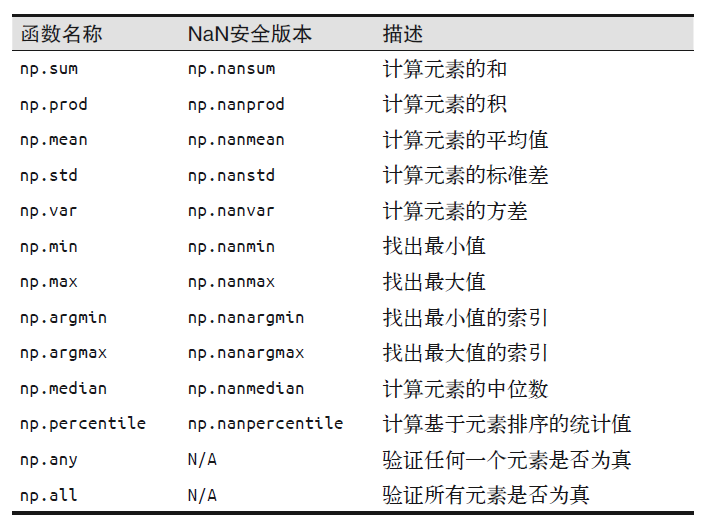
\includegraphics{03.png}

    大多数的聚合都有对 NaN
值的安全处理策略(NaN-safe),即计算时忽略所有的缺失值。

    \begin{tcolorbox}[breakable, size=fbox, boxrule=1pt, pad at break*=1mm,colback=cellbackground, colframe=cellborder]
\prompt{In}{incolor}{439}{\boxspacing}
\begin{Verbatim}[commandchars=\\\{\}]
\PY{n}{big\PYZus{}array} \PY{o}{=} \PY{n}{np}\PY{o}{.}\PY{n}{random}\PY{o}{.}\PY{n}{rand}\PY{p}{(}\PY{l+m+mi}{1000000}\PY{p}{)}
\PY{n}{big\PYZus{}array}
\end{Verbatim}
\end{tcolorbox}

            \begin{tcolorbox}[breakable, size=fbox, boxrule=.5pt, pad at break*=1mm, opacityfill=0]
\prompt{Out}{outcolor}{439}{\boxspacing}
\begin{Verbatim}[commandchars=\\\{\}]
array([0.50814981, 0.16175075, 0.29048705, {\ldots}, 0.46435639, 0.01625442,
       0.59372462])
\end{Verbatim}
\end{tcolorbox}
        
    \begin{tcolorbox}[breakable, size=fbox, boxrule=1pt, pad at break*=1mm,colback=cellbackground, colframe=cellborder]
\prompt{In}{incolor}{440}{\boxspacing}
\begin{Verbatim}[commandchars=\\\{\}]
\PY{n+nb}{min}\PY{p}{(}\PY{n}{big\PYZus{}array}\PY{p}{)}\PY{p}{,} \PY{n+nb}{max}\PY{p}{(}\PY{n}{big\PYZus{}array}\PY{p}{)}
\end{Verbatim}
\end{tcolorbox}

            \begin{tcolorbox}[breakable, size=fbox, boxrule=.5pt, pad at break*=1mm, opacityfill=0]
\prompt{Out}{outcolor}{440}{\boxspacing}
\begin{Verbatim}[commandchars=\\\{\}]
(1.2420378219246686e-06, 0.9999996092814999)
\end{Verbatim}
\end{tcolorbox}
        
    在对较大的数据进行分析时,一项基本的工作就是有效的数据累计(summarization):计算累计(aggregation)指标,如sum()、mean()、median()、min()
和max(),其中每一个指 标都呈现了大数据集的特征。

    \begin{tcolorbox}[breakable, size=fbox, boxrule=1pt, pad at break*=1mm,colback=cellbackground, colframe=cellborder]
\prompt{In}{incolor}{441}{\boxspacing}
\begin{Verbatim}[commandchars=\\\{\}]
\PY{c+c1}{\PYZsh{} seaborn 行星数据中包含了截至2014 年已被发现的一千多颗外行星的资料。}
\PY{k+kn}{import} \PY{n+nn}{seaborn} \PY{k}{as} \PY{n+nn}{sns}
\PY{n}{planets} \PY{o}{=} \PY{n}{sns}\PY{o}{.}\PY{n}{load\PYZus{}dataset}\PY{p}{(}\PY{l+s+s1}{\PYZsq{}}\PY{l+s+s1}{planets}\PY{l+s+s1}{\PYZsq{}}\PY{p}{)}
\PY{n}{planets}\PY{o}{.}\PY{n}{shape}
\end{Verbatim}
\end{tcolorbox}

            \begin{tcolorbox}[breakable, size=fbox, boxrule=.5pt, pad at break*=1mm, opacityfill=0]
\prompt{Out}{outcolor}{441}{\boxspacing}
\begin{Verbatim}[commandchars=\\\{\}]
(1035, 6)
\end{Verbatim}
\end{tcolorbox}
        
    \begin{tcolorbox}[breakable, size=fbox, boxrule=1pt, pad at break*=1mm,colback=cellbackground, colframe=cellborder]
\prompt{In}{incolor}{442}{\boxspacing}
\begin{Verbatim}[commandchars=\\\{\}]
\PY{n}{planets}\PY{o}{.}\PY{n}{head}\PY{p}{(}\PY{p}{)}
\end{Verbatim}
\end{tcolorbox}

            \begin{tcolorbox}[breakable, size=fbox, boxrule=.5pt, pad at break*=1mm, opacityfill=0]
\prompt{Out}{outcolor}{442}{\boxspacing}
\begin{Verbatim}[commandchars=\\\{\}]
            method  number  orbital\_period   mass  distance  year
0  Radial Velocity       1         269.300   7.10     77.40  2006
1  Radial Velocity       1         874.774   2.21     56.95  2008
2  Radial Velocity       1         763.000   2.60     19.84  2011
3  Radial Velocity       1         326.030  19.40    110.62  2007
4  Radial Velocity       1         516.220  10.50    119.47  2009
\end{Verbatim}
\end{tcolorbox}
        
    与一维 NumPy 数组相同,Pandas 的 Series 的累计函数也会返回一个统计值:

    \begin{tcolorbox}[breakable, size=fbox, boxrule=1pt, pad at break*=1mm,colback=cellbackground, colframe=cellborder]
\prompt{In}{incolor}{443}{\boxspacing}
\begin{Verbatim}[commandchars=\\\{\}]
\PY{n}{rng} \PY{o}{=} \PY{n}{np}\PY{o}{.}\PY{n}{random}\PY{o}{.}\PY{n}{RandomState}\PY{p}{(}\PY{l+m+mi}{42}\PY{p}{)}
\PY{n}{ser} \PY{o}{=} \PY{n}{pd}\PY{o}{.}\PY{n}{Series}\PY{p}{(}\PY{n}{rng}\PY{o}{.}\PY{n}{rand}\PY{p}{(}\PY{l+m+mi}{5}\PY{p}{)}\PY{p}{)}
\PY{n}{ser}
\end{Verbatim}
\end{tcolorbox}

            \begin{tcolorbox}[breakable, size=fbox, boxrule=.5pt, pad at break*=1mm, opacityfill=0]
\prompt{Out}{outcolor}{443}{\boxspacing}
\begin{Verbatim}[commandchars=\\\{\}]
0    0.374540
1    0.950714
2    0.731994
3    0.598658
4    0.156019
dtype: float64
\end{Verbatim}
\end{tcolorbox}
        
    \begin{tcolorbox}[breakable, size=fbox, boxrule=1pt, pad at break*=1mm,colback=cellbackground, colframe=cellborder]
\prompt{In}{incolor}{444}{\boxspacing}
\begin{Verbatim}[commandchars=\\\{\}]
\PY{n}{ser}\PY{o}{.}\PY{n}{sum}\PY{p}{(}\PY{p}{)}
\end{Verbatim}
\end{tcolorbox}

            \begin{tcolorbox}[breakable, size=fbox, boxrule=.5pt, pad at break*=1mm, opacityfill=0]
\prompt{Out}{outcolor}{444}{\boxspacing}
\begin{Verbatim}[commandchars=\\\{\}]
2.811925491708157
\end{Verbatim}
\end{tcolorbox}
        
    \begin{tcolorbox}[breakable, size=fbox, boxrule=1pt, pad at break*=1mm,colback=cellbackground, colframe=cellborder]
\prompt{In}{incolor}{445}{\boxspacing}
\begin{Verbatim}[commandchars=\\\{\}]
\PY{n}{ser}\PY{o}{.}\PY{n}{mean}\PY{p}{(}\PY{p}{)}
\end{Verbatim}
\end{tcolorbox}

            \begin{tcolorbox}[breakable, size=fbox, boxrule=.5pt, pad at break*=1mm, opacityfill=0]
\prompt{Out}{outcolor}{445}{\boxspacing}
\begin{Verbatim}[commandchars=\\\{\}]
0.5623850983416314
\end{Verbatim}
\end{tcolorbox}
        
    DataFrame 的累计函数默认对每列进行统计:

    \begin{tcolorbox}[breakable, size=fbox, boxrule=1pt, pad at break*=1mm,colback=cellbackground, colframe=cellborder]
\prompt{In}{incolor}{446}{\boxspacing}
\begin{Verbatim}[commandchars=\\\{\}]
\PY{n}{df} \PY{o}{=} \PY{n}{pd}\PY{o}{.}\PY{n}{DataFrame}\PY{p}{(}\PY{p}{\PYZob{}}\PY{l+s+s1}{\PYZsq{}}\PY{l+s+s1}{A}\PY{l+s+s1}{\PYZsq{}}\PY{p}{:} \PY{n}{rng}\PY{o}{.}\PY{n}{rand}\PY{p}{(}\PY{l+m+mi}{5}\PY{p}{)}\PY{p}{,}\PY{l+s+s1}{\PYZsq{}}\PY{l+s+s1}{B}\PY{l+s+s1}{\PYZsq{}}\PY{p}{:} \PY{n}{rng}\PY{o}{.}\PY{n}{rand}\PY{p}{(}\PY{l+m+mi}{5}\PY{p}{)}\PY{p}{\PYZcb{}}\PY{p}{)}
\PY{n}{df}
\end{Verbatim}
\end{tcolorbox}

            \begin{tcolorbox}[breakable, size=fbox, boxrule=.5pt, pad at break*=1mm, opacityfill=0]
\prompt{Out}{outcolor}{446}{\boxspacing}
\begin{Verbatim}[commandchars=\\\{\}]
          A         B
0  0.155995  0.020584
1  0.058084  0.969910
2  0.866176  0.832443
3  0.601115  0.212339
4  0.708073  0.181825
\end{Verbatim}
\end{tcolorbox}
        
    \begin{tcolorbox}[breakable, size=fbox, boxrule=1pt, pad at break*=1mm,colback=cellbackground, colframe=cellborder]
\prompt{In}{incolor}{447}{\boxspacing}
\begin{Verbatim}[commandchars=\\\{\}]
\PY{n}{df}\PY{o}{.}\PY{n}{mean}\PY{p}{(}\PY{p}{)}
\end{Verbatim}
\end{tcolorbox}

            \begin{tcolorbox}[breakable, size=fbox, boxrule=.5pt, pad at break*=1mm, opacityfill=0]
\prompt{Out}{outcolor}{447}{\boxspacing}
\begin{Verbatim}[commandchars=\\\{\}]
A    0.477888
B    0.443420
dtype: float64
\end{Verbatim}
\end{tcolorbox}
        
    设置axis 参数,可以对每一行进行统计

    \begin{tcolorbox}[breakable, size=fbox, boxrule=1pt, pad at break*=1mm,colback=cellbackground, colframe=cellborder]
\prompt{In}{incolor}{448}{\boxspacing}
\begin{Verbatim}[commandchars=\\\{\}]
\PY{n}{df}\PY{o}{.}\PY{n}{mean}\PY{p}{(}\PY{n}{axis}\PY{o}{=}\PY{l+s+s1}{\PYZsq{}}\PY{l+s+s1}{columns}\PY{l+s+s1}{\PYZsq{}}\PY{p}{)}
\end{Verbatim}
\end{tcolorbox}

            \begin{tcolorbox}[breakable, size=fbox, boxrule=.5pt, pad at break*=1mm, opacityfill=0]
\prompt{Out}{outcolor}{448}{\boxspacing}
\begin{Verbatim}[commandchars=\\\{\}]
0    0.088290
1    0.513997
2    0.849309
3    0.406727
4    0.444949
dtype: float64
\end{Verbatim}
\end{tcolorbox}
        
    Pandas 内置的一些累计方法如图所示。

    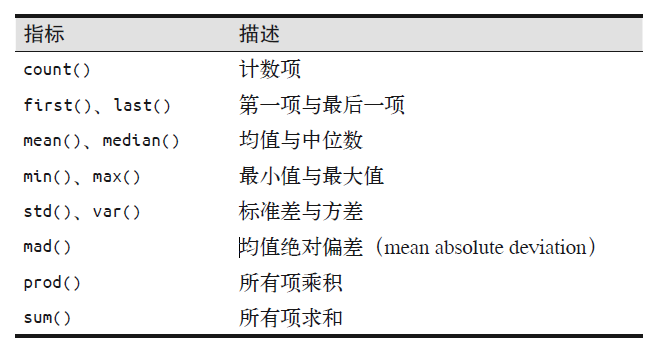
\includegraphics{04.png}

    简单的累计方法可以让我们对数据集有一个笼统的认识,但是我们经常还需要对某些标签或索引的局部进行累计分析,这时就需要用到
groupby 了。虽然``分组''(group by)这个名字是借用 SQL
数据库语言的命令,但其理念引用发明 R 语言 frame 的 Hadley Wickham
的观点可能更合适:分割(split)、应用(apply)和组合(combine)。

    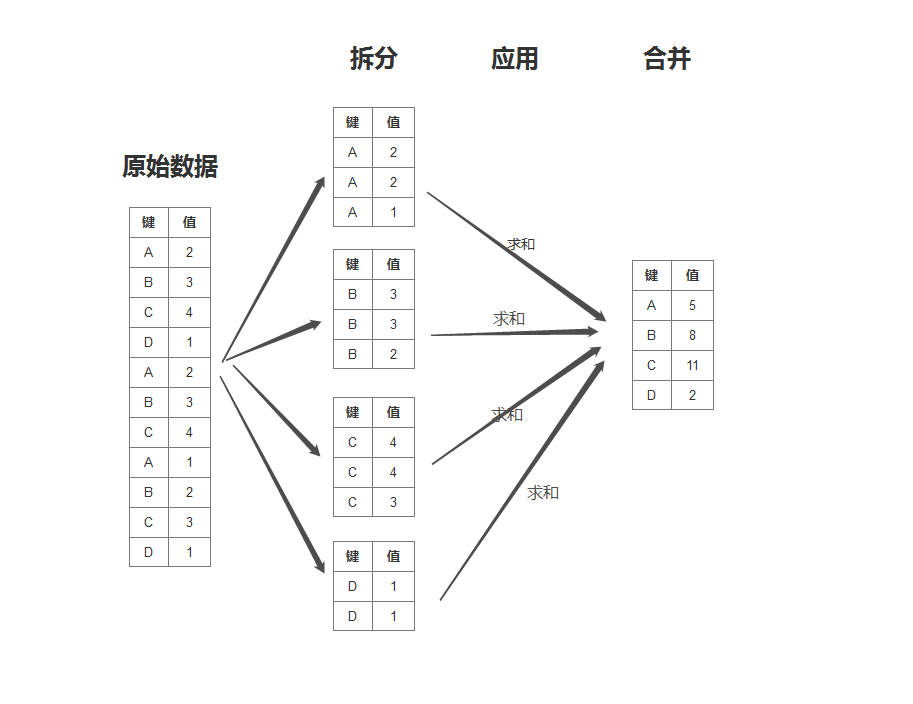
\includegraphics{05.png}

    \begin{itemize}
\tightlist
\item
  分割步骤将 DataFrame 按照指定的键分割成若干组。
\item
  应用步骤对每个组应用函数,通常是累计、转换或过滤函数。
\item
  组合步骤将每一组的结果合并成一个输出数组。
\end{itemize}

    \begin{tcolorbox}[breakable, size=fbox, boxrule=1pt, pad at break*=1mm,colback=cellbackground, colframe=cellborder]
\prompt{In}{incolor}{451}{\boxspacing}
\begin{Verbatim}[commandchars=\\\{\}]
\PY{n}{data}\PY{o}{=}\PY{n}{pd}\PY{o}{.}\PY{n}{read\PYZus{}csv}\PY{p}{(}\PY{l+s+s2}{\PYZdq{}}\PY{l+s+s2}{hw4\PYZus{}data1.csv}\PY{l+s+s2}{\PYZdq{}}\PY{p}{,}\PY{n}{encoding}\PY{o}{=}\PY{l+s+s2}{\PYZdq{}}\PY{l+s+s2}{gbk}\PY{l+s+s2}{\PYZdq{}}\PY{p}{)}
\PY{n}{data}\PY{o}{.}\PY{n}{head}\PY{p}{(}\PY{p}{)}
\end{Verbatim}
\end{tcolorbox}

            \begin{tcolorbox}[breakable, size=fbox, boxrule=.5pt, pad at break*=1mm, opacityfill=0]
\prompt{Out}{outcolor}{451}{\boxspacing}
\begin{Verbatim}[commandchars=\\\{\}]
  CLASS\_ID  STD\_ID SUBJECT  SCORE  LAST\_SCORE
0    A1231       1      语文     97          94
1    A1231       1      数学    120         124
2    A1231       1      英语    107         109
3    A1231       1      生物     86          87
4    A1231       1      化学     92          88
\end{Verbatim}
\end{tcolorbox}
        
    假如对于上面的数据我们想要分科目查看平均分

    \begin{tcolorbox}[breakable, size=fbox, boxrule=1pt, pad at break*=1mm,colback=cellbackground, colframe=cellborder]
\prompt{In}{incolor}{452}{\boxspacing}
\begin{Verbatim}[commandchars=\\\{\}]
\PY{n}{group\PYZus{}sub}\PY{o}{=}\PY{n}{data}\PY{p}{[}\PY{l+s+s2}{\PYZdq{}}\PY{l+s+s2}{SCORE}\PY{l+s+s2}{\PYZdq{}}\PY{p}{]}\PY{o}{.}\PY{n}{groupby}\PY{p}{(}\PY{n}{data}\PY{p}{[}\PY{l+s+s2}{\PYZdq{}}\PY{l+s+s2}{SUBJECT}\PY{l+s+s2}{\PYZdq{}}\PY{p}{]}\PY{p}{)}
\PY{n}{group\PYZus{}sub}
\end{Verbatim}
\end{tcolorbox}

            \begin{tcolorbox}[breakable, size=fbox, boxrule=.5pt, pad at break*=1mm, opacityfill=0]
\prompt{Out}{outcolor}{452}{\boxspacing}
\begin{Verbatim}[commandchars=\\\{\}]
<pandas.core.groupby.generic.SeriesGroupBy object at 0x000001BD911A8B88>
\end{Verbatim}
\end{tcolorbox}
        
    这里的结果只是一个groupby对象,也就是我们指示图中的拆分,想要得到运算结果需要传入想要的函数

    \begin{tcolorbox}[breakable, size=fbox, boxrule=1pt, pad at break*=1mm,colback=cellbackground, colframe=cellborder]
\prompt{In}{incolor}{453}{\boxspacing}
\begin{Verbatim}[commandchars=\\\{\}]
\PY{n}{group\PYZus{}sub}\PY{o}{.}\PY{n}{mean}\PY{p}{(}\PY{p}{)}
\end{Verbatim}
\end{tcolorbox}

            \begin{tcolorbox}[breakable, size=fbox, boxrule=.5pt, pad at break*=1mm, opacityfill=0]
\prompt{Out}{outcolor}{453}{\boxspacing}
\begin{Verbatim}[commandchars=\\\{\}]
SUBJECT
化学     85.00
数学     98.50
物理     82.50
生物     82.50
英语    102.75
语文    100.00
Name: SCORE, dtype: float64
\end{Verbatim}
\end{tcolorbox}
        
    \begin{tcolorbox}[breakable, size=fbox, boxrule=1pt, pad at break*=1mm,colback=cellbackground, colframe=cellborder]
\prompt{In}{incolor}{454}{\boxspacing}
\begin{Verbatim}[commandchars=\\\{\}]
\PY{n}{group\PYZus{}sub}\PY{o}{.}\PY{n}{sum}\PY{p}{(}\PY{p}{)}
\end{Verbatim}
\end{tcolorbox}

            \begin{tcolorbox}[breakable, size=fbox, boxrule=.5pt, pad at break*=1mm, opacityfill=0]
\prompt{Out}{outcolor}{454}{\boxspacing}
\begin{Verbatim}[commandchars=\\\{\}]
SUBJECT
化学    340
数学    394
物理    330
生物    330
英语    411
语文    400
Name: SCORE, dtype: int64
\end{Verbatim}
\end{tcolorbox}
        
    如果既要分科目也要分班级的话

    \begin{tcolorbox}[breakable, size=fbox, boxrule=1pt, pad at break*=1mm,colback=cellbackground, colframe=cellborder]
\prompt{In}{incolor}{455}{\boxspacing}
\begin{Verbatim}[commandchars=\\\{\}]
\PY{n}{data}\PY{p}{[}\PY{l+s+s2}{\PYZdq{}}\PY{l+s+s2}{SCORE}\PY{l+s+s2}{\PYZdq{}}\PY{p}{]}\PY{o}{.}\PY{n}{groupby}\PY{p}{(}\PY{p}{[}\PY{n}{data}\PY{p}{[}\PY{l+s+s2}{\PYZdq{}}\PY{l+s+s2}{CLASS\PYZus{}ID}\PY{l+s+s2}{\PYZdq{}}\PY{p}{]}\PY{p}{,}\PY{n}{data}\PY{p}{[}\PY{l+s+s2}{\PYZdq{}}\PY{l+s+s2}{SUBJECT}\PY{l+s+s2}{\PYZdq{}}\PY{p}{]}\PY{p}{]}\PY{p}{)}\PY{o}{.}\PY{n}{mean}\PY{p}{(}\PY{p}{)}
\end{Verbatim}
\end{tcolorbox}

            \begin{tcolorbox}[breakable, size=fbox, boxrule=.5pt, pad at break*=1mm, opacityfill=0]
\prompt{Out}{outcolor}{455}{\boxspacing}
\begin{Verbatim}[commandchars=\\\{\}]
CLASS\_ID  SUBJECT
A1231     化学          80.0
          数学         109.0
          物理          77.0
          生物          82.5
          英语         114.0
          语文         101.5
A1232     化学          90.0
          数学          88.0
          物理          88.0
          生物          82.5
          英语          91.5
          语文          98.5
Name: SCORE, dtype: float64
\end{Verbatim}
\end{tcolorbox}
        
    GroupBy 对象的 aggregate()、filter()、transform() 和 apply()
方法,在数据组合之前实现了大量高效的操作。

    \begin{tcolorbox}[breakable, size=fbox, boxrule=1pt, pad at break*=1mm,colback=cellbackground, colframe=cellborder]
\prompt{In}{incolor}{456}{\boxspacing}
\begin{Verbatim}[commandchars=\\\{\}]
\PY{n}{rng} \PY{o}{=} \PY{n}{np}\PY{o}{.}\PY{n}{random}\PY{o}{.}\PY{n}{RandomState}\PY{p}{(}\PY{l+m+mi}{0}\PY{p}{)}
\PY{n}{df} \PY{o}{=} \PY{n}{pd}\PY{o}{.}\PY{n}{DataFrame}\PY{p}{(}\PY{p}{\PYZob{}}\PY{l+s+s1}{\PYZsq{}}\PY{l+s+s1}{key}\PY{l+s+s1}{\PYZsq{}}\PY{p}{:} \PY{p}{[}\PY{l+s+s1}{\PYZsq{}}\PY{l+s+s1}{A}\PY{l+s+s1}{\PYZsq{}}\PY{p}{,} \PY{l+s+s1}{\PYZsq{}}\PY{l+s+s1}{B}\PY{l+s+s1}{\PYZsq{}}\PY{p}{,} \PY{l+s+s1}{\PYZsq{}}\PY{l+s+s1}{C}\PY{l+s+s1}{\PYZsq{}}\PY{p}{,} \PY{l+s+s1}{\PYZsq{}}\PY{l+s+s1}{A}\PY{l+s+s1}{\PYZsq{}}\PY{p}{,} \PY{l+s+s1}{\PYZsq{}}\PY{l+s+s1}{B}\PY{l+s+s1}{\PYZsq{}}\PY{p}{,} \PY{l+s+s1}{\PYZsq{}}\PY{l+s+s1}{C}\PY{l+s+s1}{\PYZsq{}}\PY{p}{]}\PY{p}{,}\PY{l+s+s1}{\PYZsq{}}\PY{l+s+s1}{data1}\PY{l+s+s1}{\PYZsq{}}\PY{p}{:} \PY{n+nb}{range}\PY{p}{(}\PY{l+m+mi}{6}\PY{p}{)}\PY{p}{,}\PY{l+s+s1}{\PYZsq{}}\PY{l+s+s1}{data2}\PY{l+s+s1}{\PYZsq{}}\PY{p}{:} \PY{n}{rng}\PY{o}{.}\PY{n}{randint}\PY{p}{(}\PY{l+m+mi}{0}\PY{p}{,} \PY{l+m+mi}{10}\PY{p}{,} \PY{l+m+mi}{6}\PY{p}{)}\PY{p}{\PYZcb{}}\PY{p}{,}
                  \PY{n}{columns} \PY{o}{=} \PY{p}{[}\PY{l+s+s1}{\PYZsq{}}\PY{l+s+s1}{key}\PY{l+s+s1}{\PYZsq{}}\PY{p}{,} \PY{l+s+s1}{\PYZsq{}}\PY{l+s+s1}{data1}\PY{l+s+s1}{\PYZsq{}}\PY{p}{,} \PY{l+s+s1}{\PYZsq{}}\PY{l+s+s1}{data2}\PY{l+s+s1}{\PYZsq{}}\PY{p}{]}\PY{p}{)}
\PY{n}{df}
\end{Verbatim}
\end{tcolorbox}

            \begin{tcolorbox}[breakable, size=fbox, boxrule=.5pt, pad at break*=1mm, opacityfill=0]
\prompt{Out}{outcolor}{456}{\boxspacing}
\begin{Verbatim}[commandchars=\\\{\}]
  key  data1  data2
0   A      0      5
1   B      1      0
2   C      2      3
3   A      3      3
4   B      4      7
5   C      5      9
\end{Verbatim}
\end{tcolorbox}
        
    \textbf{累计}。我们目前比较熟悉的 GroupBy 累计方法只有 sum() 和 median()
之类的简单函数,但是 aggregate()
其实可以支持更复杂的操作,比如字符串、函数或者函数列表,并且能一次性计算所有累计值。

    \begin{tcolorbox}[breakable, size=fbox, boxrule=1pt, pad at break*=1mm,colback=cellbackground, colframe=cellborder]
\prompt{In}{incolor}{457}{\boxspacing}
\begin{Verbatim}[commandchars=\\\{\}]
\PY{n}{df}\PY{o}{.}\PY{n}{groupby}\PY{p}{(}\PY{l+s+s1}{\PYZsq{}}\PY{l+s+s1}{key}\PY{l+s+s1}{\PYZsq{}}\PY{p}{)}\PY{o}{.}\PY{n}{aggregate}\PY{p}{(}\PY{p}{[}\PY{l+s+s1}{\PYZsq{}}\PY{l+s+s1}{min}\PY{l+s+s1}{\PYZsq{}}\PY{p}{,} \PY{n}{np}\PY{o}{.}\PY{n}{median}\PY{p}{,} \PY{n+nb}{max}\PY{p}{]}\PY{p}{)}
\end{Verbatim}
\end{tcolorbox}

            \begin{tcolorbox}[breakable, size=fbox, boxrule=.5pt, pad at break*=1mm, opacityfill=0]
\prompt{Out}{outcolor}{457}{\boxspacing}
\begin{Verbatim}[commandchars=\\\{\}]
    data1            data2
      min median max   min median max
key
A       0    1.5   3     3    4.0   5
B       1    2.5   4     0    3.5   7
C       2    3.5   5     3    6.0   9
\end{Verbatim}
\end{tcolorbox}
        
    另一种用法就是通过Python 字典指定不同列需要累计的函数:

    \begin{tcolorbox}[breakable, size=fbox, boxrule=1pt, pad at break*=1mm,colback=cellbackground, colframe=cellborder]
\prompt{In}{incolor}{458}{\boxspacing}
\begin{Verbatim}[commandchars=\\\{\}]
\PY{n}{df}\PY{o}{.}\PY{n}{groupby}\PY{p}{(}\PY{l+s+s1}{\PYZsq{}}\PY{l+s+s1}{key}\PY{l+s+s1}{\PYZsq{}}\PY{p}{)}\PY{o}{.}\PY{n}{aggregate}\PY{p}{(}\PY{p}{\PYZob{}}\PY{l+s+s1}{\PYZsq{}}\PY{l+s+s1}{data1}\PY{l+s+s1}{\PYZsq{}}\PY{p}{:} \PY{l+s+s1}{\PYZsq{}}\PY{l+s+s1}{min}\PY{l+s+s1}{\PYZsq{}}\PY{p}{,}\PY{l+s+s1}{\PYZsq{}}\PY{l+s+s1}{data2}\PY{l+s+s1}{\PYZsq{}}\PY{p}{:} \PY{l+s+s1}{\PYZsq{}}\PY{l+s+s1}{max}\PY{l+s+s1}{\PYZsq{}}\PY{p}{\PYZcb{}}\PY{p}{)}
\end{Verbatim}
\end{tcolorbox}

            \begin{tcolorbox}[breakable, size=fbox, boxrule=.5pt, pad at break*=1mm, opacityfill=0]
\prompt{Out}{outcolor}{458}{\boxspacing}
\begin{Verbatim}[commandchars=\\\{\}]
     data1  data2
key
A        0      5
B        1      7
C        2      9
\end{Verbatim}
\end{tcolorbox}
        
    \textbf{过滤}。过滤操作可以让你按照分组的属性丢弃若干数据。例如,我们可能只需要保留标准差超过某个阈值的组:

    \begin{tcolorbox}[breakable, size=fbox, boxrule=1pt, pad at break*=1mm,colback=cellbackground, colframe=cellborder]
\prompt{In}{incolor}{459}{\boxspacing}
\begin{Verbatim}[commandchars=\\\{\}]
\PY{k}{def} \PY{n+nf}{filter\PYZus{}func}\PY{p}{(}\PY{n}{x}\PY{p}{)}\PY{p}{:}
    \PY{k}{return} \PY{n}{x}\PY{p}{[}\PY{l+s+s1}{\PYZsq{}}\PY{l+s+s1}{data2}\PY{l+s+s1}{\PYZsq{}}\PY{p}{]}\PY{o}{.}\PY{n}{std}\PY{p}{(}\PY{p}{)} \PY{o}{\PYZgt{}} \PY{l+m+mi}{4}
\PY{n}{df} 
\end{Verbatim}
\end{tcolorbox}

            \begin{tcolorbox}[breakable, size=fbox, boxrule=.5pt, pad at break*=1mm, opacityfill=0]
\prompt{Out}{outcolor}{459}{\boxspacing}
\begin{Verbatim}[commandchars=\\\{\}]
  key  data1  data2
0   A      0      5
1   B      1      0
2   C      2      3
3   A      3      3
4   B      4      7
5   C      5      9
\end{Verbatim}
\end{tcolorbox}
        
    \begin{tcolorbox}[breakable, size=fbox, boxrule=1pt, pad at break*=1mm,colback=cellbackground, colframe=cellborder]
\prompt{In}{incolor}{460}{\boxspacing}
\begin{Verbatim}[commandchars=\\\{\}]
\PY{n}{df}\PY{o}{.}\PY{n}{groupby}\PY{p}{(}\PY{l+s+s1}{\PYZsq{}}\PY{l+s+s1}{key}\PY{l+s+s1}{\PYZsq{}}\PY{p}{)}\PY{o}{.}\PY{n}{std}\PY{p}{(}\PY{p}{)}
\end{Verbatim}
\end{tcolorbox}

            \begin{tcolorbox}[breakable, size=fbox, boxrule=.5pt, pad at break*=1mm, opacityfill=0]
\prompt{Out}{outcolor}{460}{\boxspacing}
\begin{Verbatim}[commandchars=\\\{\}]
       data1     data2
key
A    2.12132  1.414214
B    2.12132  4.949747
C    2.12132  4.242641
\end{Verbatim}
\end{tcolorbox}
        
    \begin{tcolorbox}[breakable, size=fbox, boxrule=1pt, pad at break*=1mm,colback=cellbackground, colframe=cellborder]
\prompt{In}{incolor}{461}{\boxspacing}
\begin{Verbatim}[commandchars=\\\{\}]
\PY{n}{df}\PY{o}{.}\PY{n}{groupby}\PY{p}{(}\PY{l+s+s1}{\PYZsq{}}\PY{l+s+s1}{key}\PY{l+s+s1}{\PYZsq{}}\PY{p}{)}\PY{o}{.}\PY{n}{filter}\PY{p}{(}\PY{n}{filter\PYZus{}func}\PY{p}{)}
\end{Verbatim}
\end{tcolorbox}

            \begin{tcolorbox}[breakable, size=fbox, boxrule=.5pt, pad at break*=1mm, opacityfill=0]
\prompt{Out}{outcolor}{461}{\boxspacing}
\begin{Verbatim}[commandchars=\\\{\}]
  key  data1  data2
1   B      1      0
2   C      2      3
4   B      4      7
5   C      5      9
\end{Verbatim}
\end{tcolorbox}
        
    filter() 函数会返回一个布尔值,表示每个组是否通过过滤。由于 A 组 `data2'
列的标准差不大于4,所以被丢弃了。

    \textbf{转换}。累计操作返回的是对组内全量数据缩减过的结果,而转换操作会返回一个新的全量数据。数据经过转换之后,其形状与原来的输入数据是一样的。常见的例子就是将每
一组的样本数据减去各组的均值,实现数据标准化:

    \begin{tcolorbox}[breakable, size=fbox, boxrule=1pt, pad at break*=1mm,colback=cellbackground, colframe=cellborder]
\prompt{In}{incolor}{462}{\boxspacing}
\begin{Verbatim}[commandchars=\\\{\}]
\PY{n}{df}\PY{o}{.}\PY{n}{groupby}\PY{p}{(}\PY{l+s+s1}{\PYZsq{}}\PY{l+s+s1}{key}\PY{l+s+s1}{\PYZsq{}}\PY{p}{)}\PY{o}{.}\PY{n}{transform}\PY{p}{(}\PY{k}{lambda} \PY{n}{x}\PY{p}{:} \PY{n}{x} \PY{o}{\PYZhy{}} \PY{n}{x}\PY{o}{.}\PY{n}{mean}\PY{p}{(}\PY{p}{)}\PY{p}{)}
\end{Verbatim}
\end{tcolorbox}

            \begin{tcolorbox}[breakable, size=fbox, boxrule=.5pt, pad at break*=1mm, opacityfill=0]
\prompt{Out}{outcolor}{462}{\boxspacing}
\begin{Verbatim}[commandchars=\\\{\}]
   data1  data2
0   -1.5    1.0
1   -1.5   -3.5
2   -1.5   -3.0
3    1.5   -1.0
4    1.5    3.5
5    1.5    3.0
\end{Verbatim}
\end{tcolorbox}
        
    \textbf{apply() 方法}。apply()
方法让你可以在每个组上应用任意方法。这个函数输入一个 DataFrame,返回一个
Pandas 对象(DataFrame
或Series)或一个标量(scalar,单个数值)。组合操作会适应返回结果类型。

    \begin{tcolorbox}[breakable, size=fbox, boxrule=1pt, pad at break*=1mm,colback=cellbackground, colframe=cellborder]
\prompt{In}{incolor}{463}{\boxspacing}
\begin{Verbatim}[commandchars=\\\{\}]
\PY{c+c1}{\PYZsh{} 将第一列数据以第二列的和为基数进行标准化}
\PY{k}{def} \PY{n+nf}{norm\PYZus{}by\PYZus{}data2}\PY{p}{(}\PY{n}{x}\PY{p}{)}\PY{p}{:}
    \PY{c+c1}{\PYZsh{} x是一个分组数据的DataFrame}
    \PY{n}{x}\PY{p}{[}\PY{l+s+s1}{\PYZsq{}}\PY{l+s+s1}{data1}\PY{l+s+s1}{\PYZsq{}}\PY{p}{]} \PY{o}{/}\PY{o}{=} \PY{n}{x}\PY{p}{[}\PY{l+s+s1}{\PYZsq{}}\PY{l+s+s1}{data2}\PY{l+s+s1}{\PYZsq{}}\PY{p}{]}\PY{o}{.}\PY{n}{sum}\PY{p}{(}\PY{p}{)}
    \PY{k}{return} \PY{n}{x}
\PY{n}{df}\PY{o}{.}\PY{n}{groupby}\PY{p}{(}\PY{l+s+s1}{\PYZsq{}}\PY{l+s+s1}{key}\PY{l+s+s1}{\PYZsq{}}\PY{p}{)}\PY{o}{.}\PY{n}{apply}\PY{p}{(}\PY{n}{norm\PYZus{}by\PYZus{}data2}\PY{p}{)}
\end{Verbatim}
\end{tcolorbox}

            \begin{tcolorbox}[breakable, size=fbox, boxrule=.5pt, pad at break*=1mm, opacityfill=0]
\prompt{Out}{outcolor}{463}{\boxspacing}
\begin{Verbatim}[commandchars=\\\{\}]
  key     data1  data2
0   A  0.000000      5
1   B  0.142857      0
2   C  0.166667      3
3   A  0.375000      3
4   B  0.571429      7
5   C  0.416667      9
\end{Verbatim}
\end{tcolorbox}
        
    GroupBy 里的 apply()
方法非常灵活,唯一需要注意的地方是它总是输入分组数据的 DataFrame,返回
Pandas 对象或标量。具体如何选择需要视情况而定。

    \hypertarget{ux95eeux9898ux4e8c-knn-model}{%
\subsection{问题二 KNN Model}\label{ux95eeux9898ux4e8c-knn-model}}

    【2】
利用iris.csv数据集,建立KNN模型,预测Sepal.Length/Sepal.Width/Petal.Length/Petal.Width分别为(6.3,3.1,4.8,1.4)时,属于鸢尾花的哪个类别?编写KNN源代码。

    \begin{tcolorbox}[breakable, size=fbox, boxrule=1pt, pad at break*=1mm,colback=cellbackground, colframe=cellborder]
\prompt{In}{incolor}{464}{\boxspacing}
\begin{Verbatim}[commandchars=\\\{\}]
\PY{n}{data}\PY{o}{=}\PY{n}{pd}\PY{o}{.}\PY{n}{read\PYZus{}csv}\PY{p}{(}\PY{l+s+s2}{\PYZdq{}}\PY{l+s+s2}{HW4\PYZus{}DATA2.csv}\PY{l+s+s2}{\PYZdq{}}\PY{p}{,}\PY{n}{index\PYZus{}col}\PY{o}{=}\PY{l+s+s2}{\PYZdq{}}\PY{l+s+s2}{index}\PY{l+s+s2}{\PYZdq{}}\PY{p}{)}
\PY{n}{data}
\end{Verbatim}
\end{tcolorbox}

            \begin{tcolorbox}[breakable, size=fbox, boxrule=.5pt, pad at break*=1mm, opacityfill=0]
\prompt{Out}{outcolor}{464}{\boxspacing}
\begin{Verbatim}[commandchars=\\\{\}]
       Sepal.Length  Sepal.Width  Pepal.Length  Pepal.Width     Species
index
1               5.1          3.5           1.4          0.2      setosa
2               4.9          3.0           1.4          0.2      setosa
3               4.7          3.2           1.3          0.2      setosa
4               4.6          3.1           1.5          0.2      setosa
48              4.6          3.2           1.4          0.2      setosa
49              5.3          3.7           1.5          0.2      setosa
50              5.0          3.3           1.4          0.2      setosa
51              7.0          3.2           4.7          1.4  versicolor
52              6.4          3.2           4.5          1.5  versicolor
53              6.9          3.1           4.9          1.5  versicolor
59              6.6          2.9           4.6          1.3  versicolor
118             7.7          3.8           6.7          2.2   virginica
119             7.7          2.6           6.9          2.3   virginica
\end{Verbatim}
\end{tcolorbox}
        
    \begin{tcolorbox}[breakable, size=fbox, boxrule=1pt, pad at break*=1mm,colback=cellbackground, colframe=cellborder]
\prompt{In}{incolor}{465}{\boxspacing}
\begin{Verbatim}[commandchars=\\\{\}]
\PY{n}{labels}\PY{o}{=}\PY{n}{data}\PY{o}{.}\PY{n}{pop}\PY{p}{(}\PY{l+s+s2}{\PYZdq{}}\PY{l+s+s2}{Species}\PY{l+s+s2}{\PYZdq{}}\PY{p}{)}
\PY{n}{labels}\PY{o}{=}\PY{n}{np}\PY{o}{.}\PY{n}{array}\PY{p}{(}\PY{n}{labels}\PY{p}{)}
\PY{n}{labels}
\end{Verbatim}
\end{tcolorbox}

            \begin{tcolorbox}[breakable, size=fbox, boxrule=.5pt, pad at break*=1mm, opacityfill=0]
\prompt{Out}{outcolor}{465}{\boxspacing}
\begin{Verbatim}[commandchars=\\\{\}]
array(['setosa', 'setosa', 'setosa', 'setosa', 'setosa', 'setosa',
       'setosa', 'versicolor', 'versicolor', 'versicolor', 'versicolor',
       'virginica', 'virginica'], dtype=object)
\end{Verbatim}
\end{tcolorbox}
        
    \begin{tcolorbox}[breakable, size=fbox, boxrule=1pt, pad at break*=1mm,colback=cellbackground, colframe=cellborder]
\prompt{In}{incolor}{466}{\boxspacing}
\begin{Verbatim}[commandchars=\\\{\}]
\PY{c+c1}{\PYZsh{}print(type(data.loc[1,:]))}
\PY{n}{data}\PY{o}{=}\PY{n}{np}\PY{o}{.}\PY{n}{array}\PY{p}{(}\PY{n}{data}\PY{p}{)}
\PY{n}{data}
\end{Verbatim}
\end{tcolorbox}

            \begin{tcolorbox}[breakable, size=fbox, boxrule=.5pt, pad at break*=1mm, opacityfill=0]
\prompt{Out}{outcolor}{466}{\boxspacing}
\begin{Verbatim}[commandchars=\\\{\}]
array([[5.1, 3.5, 1.4, 0.2],
       [4.9, 3. , 1.4, 0.2],
       [4.7, 3.2, 1.3, 0.2],
       [4.6, 3.1, 1.5, 0.2],
       [4.6, 3.2, 1.4, 0.2],
       [5.3, 3.7, 1.5, 0.2],
       [5. , 3.3, 1.4, 0.2],
       [7. , 3.2, 4.7, 1.4],
       [6.4, 3.2, 4.5, 1.5],
       [6.9, 3.1, 4.9, 1.5],
       [6.6, 2.9, 4.6, 1.3],
       [7.7, 3.8, 6.7, 2.2],
       [7.7, 2.6, 6.9, 2.3]])
\end{Verbatim}
\end{tcolorbox}
        
    \begin{tcolorbox}[breakable, size=fbox, boxrule=1pt, pad at break*=1mm,colback=cellbackground, colframe=cellborder]
\prompt{In}{incolor}{467}{\boxspacing}
\begin{Verbatim}[commandchars=\\\{\}]
\PY{k+kn}{from} \PY{n+nn}{numpy} \PY{k}{import} \PY{o}{*}
\PY{n}{new\PYZus{}t}\PY{o}{=}\PY{n}{np}\PY{o}{.}\PY{n}{array}\PY{p}{(}\PY{p}{[}\PY{l+m+mf}{6.3}\PY{p}{,}\PY{l+m+mf}{3.1}\PY{p}{,}\PY{l+m+mf}{4.8}\PY{p}{,}\PY{l+m+mf}{1.4}\PY{p}{]}\PY{p}{)}

\PY{n}{numSamples} \PY{o}{=} \PY{n}{data}\PY{o}{.}\PY{n}{shape}\PY{p}{[}\PY{l+m+mi}{0}\PY{p}{]}
\PY{n}{diff}\PY{o}{=}\PY{n}{tile}\PY{p}{(}\PY{n}{new\PYZus{}t}\PY{p}{,}\PY{p}{(}\PY{n}{numSamples}\PY{p}{,}\PY{l+m+mi}{1}\PY{p}{)}\PY{p}{)}\PY{o}{\PYZhy{}}\PY{n}{data} \PY{c+c1}{\PYZsh{}重复数组}
\PY{n}{squreDiff} \PY{o}{=} \PY{n}{diff}\PY{o}{*}\PY{o}{*}\PY{l+m+mi}{2}
\PY{n}{squreDist} \PY{o}{=} \PY{n+nb}{sum}\PY{p}{(}\PY{n}{squreDiff}\PY{p}{,} \PY{n}{axis}\PY{o}{=}\PY{l+m+mi}{1}\PY{p}{)}
\PY{n}{distance} \PY{o}{=} \PY{n}{squreDist} \PY{o}{*}\PY{o}{*} \PY{l+m+mf}{0.5}
\PY{n}{distance}
\end{Verbatim}
\end{tcolorbox}

            \begin{tcolorbox}[breakable, size=fbox, boxrule=.5pt, pad at break*=1mm, opacityfill=0]
\prompt{Out}{outcolor}{467}{\boxspacing}
\begin{Verbatim}[commandchars=\\\{\}]
array([3.82099463, 3.86910842, 4.03236903, 3.90128184, 3.98748041,
       3.7       , 3.83796821, 0.71414284, 0.34641016, 0.6164414 ,
       0.42426407, 2.58843582, 2.72580263])
\end{Verbatim}
\end{tcolorbox}
        
    \begin{tcolorbox}[breakable, size=fbox, boxrule=1pt, pad at break*=1mm,colback=cellbackground, colframe=cellborder]
\prompt{In}{incolor}{468}{\boxspacing}
\begin{Verbatim}[commandchars=\\\{\}]
\PY{n}{sortedDistIndices} \PY{o}{=} \PY{n}{argsort}\PY{p}{(}\PY{n}{distance}\PY{p}{)}
\PY{n}{sortedDistIndices}
\end{Verbatim}
\end{tcolorbox}

            \begin{tcolorbox}[breakable, size=fbox, boxrule=.5pt, pad at break*=1mm, opacityfill=0]
\prompt{Out}{outcolor}{468}{\boxspacing}
\begin{Verbatim}[commandchars=\\\{\}]
array([ 8, 10,  9,  7, 11, 12,  5,  0,  6,  1,  3,  4,  2], dtype=int64)
\end{Verbatim}
\end{tcolorbox}
        
    \begin{tcolorbox}[breakable, size=fbox, boxrule=1pt, pad at break*=1mm,colback=cellbackground, colframe=cellborder]
\prompt{In}{incolor}{469}{\boxspacing}
\begin{Verbatim}[commandchars=\\\{\}]
\PY{n}{classCount} \PY{o}{=} \PY{p}{\PYZob{}}\PY{p}{\PYZcb{}}
\PY{n}{K} \PY{o}{=} \PY{l+m+mi}{4}
\PY{k}{for} \PY{n}{i} \PY{o+ow}{in} \PY{n+nb}{range}\PY{p}{(}\PY{n}{K}\PY{p}{)}\PY{p}{:}
    \PY{n}{voteLabel} \PY{o}{=} \PY{n}{labels}\PY{p}{[}\PY{n}{sortedDistIndices}\PY{p}{[}\PY{n}{i}\PY{p}{]}\PY{p}{]}
    \PY{n+nb}{print}\PY{p}{(}\PY{n}{voteLabel}\PY{p}{)}
    \PY{n}{classCount}\PY{p}{[}\PY{n}{voteLabel}\PY{p}{]} \PY{o}{=} \PY{n}{classCount}\PY{o}{.}\PY{n}{get}\PY{p}{(}\PY{n}{voteLabel}\PY{p}{,} \PY{l+m+mi}{0}\PY{p}{)} \PY{o}{+} \PY{l+m+mi}{1}
\PY{n+nb}{print}\PY{p}{(}\PY{n}{classCount}\PY{p}{)}

\PY{n}{maxCount} \PY{o}{=} \PY{l+m+mi}{0}
\PY{k}{for} \PY{n}{k}\PY{p}{,} \PY{n}{v} \PY{o+ow}{in} \PY{n}{classCount}\PY{o}{.}\PY{n}{items}\PY{p}{(}\PY{p}{)}\PY{p}{:}
    \PY{k}{if} \PY{n}{v} \PY{o}{\PYZgt{}} \PY{n}{maxCount}\PY{p}{:}
        \PY{n}{maxCount} \PY{o}{=} \PY{n}{v}
        \PY{n}{maxIndex} \PY{o}{=} \PY{n}{k}

\PY{n+nb}{print}\PY{p}{(}\PY{l+s+s2}{\PYZdq{}}\PY{l+s+s2}{Your input is:}\PY{l+s+s2}{\PYZdq{}}\PY{p}{,} \PY{n}{new\PYZus{}t}\PY{p}{,} \PY{l+s+s2}{\PYZdq{}}\PY{l+s+s2}{and classified to class: }\PY{l+s+s2}{\PYZdq{}}\PY{p}{,} \PY{n}{maxIndex}\PY{p}{)}
\end{Verbatim}
\end{tcolorbox}

    \begin{Verbatim}[commandchars=\\\{\}]
versicolor
versicolor
versicolor
versicolor
\{'versicolor': 4\}
Your input is: [6.3 3.1 4.8 1.4] and classified to class:  versicolor
    \end{Verbatim}

    \hypertarget{ux95eeux9898ux4e09-ux5e38ux7528ux8dddux79bb}{%
\subsection{问题三
常用距离}\label{ux95eeux9898ux4e09-ux5e38ux7528ux8dddux79bb}}

    【3】 计算X = {[}1,2,3{]}和Y = {[}0,1,2{]}的曼哈顿距离(Manhattan
Distance),切比雪夫距离
,闵可夫斯基距离,标准化欧氏距离,马氏距离。给出计算公式,并根据公式计算。利用Python实现上述距离。

    \hypertarget{ux66fcux54c8ux987fux8dddux79bbmanhattan-distance}{%
\subsubsection{曼哈顿距离((Manhattan
Distance))}\label{ux66fcux54c8ux987fux8dddux79bbmanhattan-distance}}

    \[d(x,y)=\sqrt{\sum\limits_{k=1}^n|x_k-y_k|}\]

    \begin{tcolorbox}[breakable, size=fbox, boxrule=1pt, pad at break*=1mm,colback=cellbackground, colframe=cellborder]
\prompt{In}{incolor}{470}{\boxspacing}
\begin{Verbatim}[commandchars=\\\{\}]
\PY{k+kn}{import} \PY{n+nn}{matplotlib}\PY{n+nn}{.}\PY{n+nn}{pyplot} \PY{k}{as} \PY{n+nn}{plt}
\PY{k+kn}{from} \PY{n+nn}{mpl\PYZus{}toolkits}\PY{n+nn}{.}\PY{n+nn}{mplot3d} \PY{k}{import} \PY{n}{Axes3D}
\PY{k+kn}{from} \PY{n+nn}{mpl\PYZus{}toolkits}\PY{n+nn}{.}\PY{n+nn}{mplot3d} \PY{k}{import} \PY{n}{proj3d}
\PY{k+kn}{import} \PY{n+nn}{math}
\PY{k}{def} \PY{n+nf}{Manhattan\PYZus{}Dist}\PY{p}{(}\PY{n}{X}\PY{p}{,}\PY{n}{Y}\PY{p}{)}\PY{p}{:}
    \PY{k}{return} \PY{n}{math}\PY{o}{.}\PY{n}{sqrt}\PY{p}{(}\PY{n+nb}{sum}\PY{p}{(}\PY{p}{[}\PY{n+nb}{abs}\PY{p}{(}\PY{n}{x}\PY{o}{\PYZhy{}}\PY{n}{y}\PY{p}{)} \PY{k}{for} \PY{p}{(}\PY{n}{x}\PY{p}{,}\PY{n}{y}\PY{p}{)} \PY{o+ow}{in} \PY{n+nb}{zip}\PY{p}{(}\PY{n}{X}\PY{p}{,}\PY{n}{Y}\PY{p}{)}\PY{p}{]}\PY{p}{)}\PY{p}{)}
\end{Verbatim}
\end{tcolorbox}

    \begin{tcolorbox}[breakable, size=fbox, boxrule=1pt, pad at break*=1mm,colback=cellbackground, colframe=cellborder]
\prompt{In}{incolor}{471}{\boxspacing}
\begin{Verbatim}[commandchars=\\\{\}]
\PY{n}{X}\PY{o}{=}\PY{p}{[}\PY{l+m+mi}{1}\PY{p}{,}\PY{l+m+mi}{2}\PY{p}{,}\PY{l+m+mi}{3}\PY{p}{]}
\PY{n}{Y}\PY{o}{=}\PY{p}{[}\PY{l+m+mi}{0}\PY{p}{,}\PY{l+m+mi}{1}\PY{p}{,}\PY{l+m+mi}{2}\PY{p}{]}
\end{Verbatim}
\end{tcolorbox}

    \begin{tcolorbox}[breakable, size=fbox, boxrule=1pt, pad at break*=1mm,colback=cellbackground, colframe=cellborder]
\prompt{In}{incolor}{472}{\boxspacing}
\begin{Verbatim}[commandchars=\\\{\}]
\PY{n}{Manhattan\PYZus{}Dist}\PY{p}{(}\PY{n}{X}\PY{p}{,}\PY{n}{Y}\PY{p}{)}
\end{Verbatim}
\end{tcolorbox}

            \begin{tcolorbox}[breakable, size=fbox, boxrule=.5pt, pad at break*=1mm, opacityfill=0]
\prompt{Out}{outcolor}{472}{\boxspacing}
\begin{Verbatim}[commandchars=\\\{\}]
1.7320508075688772
\end{Verbatim}
\end{tcolorbox}
        
    \begin{tcolorbox}[breakable, size=fbox, boxrule=1pt, pad at break*=1mm,colback=cellbackground, colframe=cellborder]
\prompt{In}{incolor}{473}{\boxspacing}
\begin{Verbatim}[commandchars=\\\{\}]
\PY{n}{fig}\PY{o}{=}\PY{n}{plt}\PY{o}{.}\PY{n}{figure}\PY{p}{(}\PY{n}{figsize}\PY{o}{=}\PY{p}{(}\PY{l+m+mi}{7}\PY{p}{,}\PY{l+m+mi}{7}\PY{p}{)}\PY{p}{)}
\PY{n}{ax}\PY{o}{=}\PY{n}{fig}\PY{o}{.}\PY{n}{add\PYZus{}subplot}\PY{p}{(}\PY{l+m+mi}{111}\PY{p}{,}\PY{n}{projection}\PY{o}{=}\PY{l+s+s1}{\PYZsq{}}\PY{l+s+s1}{3d}\PY{l+s+s1}{\PYZsq{}}\PY{p}{)}
\PY{n}{ax}\PY{o}{.}\PY{n}{scatter}\PY{p}{(}\PY{p}{(}\PY{n}{X}\PY{p}{[}\PY{l+m+mi}{0}\PY{p}{]}\PY{p}{,}\PY{n}{Y}\PY{p}{[}\PY{l+m+mi}{0}\PY{p}{]}\PY{p}{)}\PY{p}{,}\PY{p}{(}\PY{n}{X}\PY{p}{[}\PY{l+m+mi}{1}\PY{p}{]}\PY{p}{,}\PY{n}{Y}\PY{p}{[}\PY{l+m+mi}{1}\PY{p}{]}\PY{p}{)}\PY{p}{,}\PY{p}{(}\PY{n}{X}\PY{p}{[}\PY{l+m+mi}{2}\PY{p}{]}\PY{p}{,}\PY{n}{Y}\PY{p}{[}\PY{l+m+mi}{2}\PY{p}{]}\PY{p}{)}\PY{p}{,}\PY{n}{color}\PY{o}{=}\PY{l+s+s1}{\PYZsq{}}\PY{l+s+s1}{b}\PY{l+s+s1}{\PYZsq{}}\PY{p}{,}\PY{n}{s}\PY{o}{=}\PY{l+m+mi}{50}\PY{p}{)}
\PY{n}{ax}\PY{o}{.}\PY{n}{plot}\PY{p}{(}\PY{p}{(}\PY{n}{X}\PY{p}{[}\PY{l+m+mi}{0}\PY{p}{]}\PY{p}{,}\PY{n}{Y}\PY{p}{[}\PY{l+m+mi}{0}\PY{p}{]}\PY{p}{)}\PY{p}{,}\PY{p}{(}\PY{n}{X}\PY{p}{[}\PY{l+m+mi}{1}\PY{p}{]}\PY{p}{,}\PY{n}{Y}\PY{p}{[}\PY{l+m+mi}{1}\PY{p}{]}\PY{p}{)}\PY{p}{,}\PY{p}{(}\PY{n}{X}\PY{p}{[}\PY{l+m+mi}{2}\PY{p}{]}\PY{p}{,}\PY{n}{Y}\PY{p}{[}\PY{l+m+mi}{2}\PY{p}{]}\PY{p}{)}\PY{p}{,}\PY{n}{color}\PY{o}{=}\PY{l+s+s1}{\PYZsq{}}\PY{l+s+s1}{r}\PY{l+s+s1}{\PYZsq{}}\PY{p}{)}
\end{Verbatim}
\end{tcolorbox}

            \begin{tcolorbox}[breakable, size=fbox, boxrule=.5pt, pad at break*=1mm, opacityfill=0]
\prompt{Out}{outcolor}{473}{\boxspacing}
\begin{Verbatim}[commandchars=\\\{\}]
[<mpl\_toolkits.mplot3d.art3d.Line3D at 0x1bd93b82f48>]
\end{Verbatim}
\end{tcolorbox}
        
    \begin{center}
    \adjustimage{max size={0.9\linewidth}{0.9\paperheight}}{output_344_1.png}
    \end{center}
    { \hspace*{\fill} \\}
    
    \hypertarget{ux5207ux6bd4ux96eaux592bux8dddux79bbchebyshev-distance}{%
\subsubsection{切比雪夫距离(Chebyshev
Distance)}\label{ux5207ux6bd4ux96eaux592bux8dddux79bbchebyshev-distance}}

    \[d(x,y)=\max\limits_{k=1}^n|x_k-y_k|\]

    \begin{tcolorbox}[breakable, size=fbox, boxrule=1pt, pad at break*=1mm,colback=cellbackground, colframe=cellborder]
\prompt{In}{incolor}{474}{\boxspacing}
\begin{Verbatim}[commandchars=\\\{\}]
\PY{k}{def} \PY{n+nf}{Chebyshev\PYZus{}Dist}\PY{p}{(}\PY{n}{X}\PY{p}{,}\PY{n}{Y}\PY{p}{)}\PY{p}{:}
    \PY{k}{return} \PY{n+nb}{max}\PY{p}{(}\PY{p}{[}\PY{n+nb}{abs}\PY{p}{(}\PY{n}{x}\PY{o}{\PYZhy{}}\PY{n}{y}\PY{p}{)} \PY{k}{for} \PY{p}{(}\PY{n}{x}\PY{p}{,}\PY{n}{y}\PY{p}{)} \PY{o+ow}{in} \PY{n+nb}{zip}\PY{p}{(}\PY{n}{X}\PY{p}{,}\PY{n}{Y}\PY{p}{)}\PY{p}{]}\PY{p}{)}
\end{Verbatim}
\end{tcolorbox}

    \begin{tcolorbox}[breakable, size=fbox, boxrule=1pt, pad at break*=1mm,colback=cellbackground, colframe=cellborder]
\prompt{In}{incolor}{475}{\boxspacing}
\begin{Verbatim}[commandchars=\\\{\}]
\PY{n}{Chebyshev\PYZus{}Dist}\PY{p}{(}\PY{n}{X}\PY{p}{,}\PY{n}{Y}\PY{p}{)}
\end{Verbatim}
\end{tcolorbox}

            \begin{tcolorbox}[breakable, size=fbox, boxrule=.5pt, pad at break*=1mm, opacityfill=0]
\prompt{Out}{outcolor}{475}{\boxspacing}
\begin{Verbatim}[commandchars=\\\{\}]
1
\end{Verbatim}
\end{tcolorbox}
        
    \hypertarget{ux95f5ux53efux592bux65afux57faux8dddux79bbminkowski-distance}{%
\subsubsection{闵可夫斯基距离(Minkowski
Distance)}\label{ux95f5ux53efux592bux65afux57faux8dddux79bbminkowski-distance}}

    \[d(x,y)=\sqrt[p]{\sum\limits_{k=1}^n|x_k-y_k|^p}\]

    \(p=1:曼哈顿距离\\ p=2:欧式距离\\ p \rightarrow \infty:切比雪夫距离\)

    \begin{tcolorbox}[breakable, size=fbox, boxrule=1pt, pad at break*=1mm,colback=cellbackground, colframe=cellborder]
\prompt{In}{incolor}{476}{\boxspacing}
\begin{Verbatim}[commandchars=\\\{\}]
\PY{k}{def} \PY{n+nf}{Minkowski\PYZus{}Dist}\PY{p}{(}\PY{n}{X}\PY{p}{,} \PY{n}{Y}\PY{p}{,} \PY{n}{p}\PY{p}{)}\PY{p}{:}
    \PY{k}{return} \PY{p}{(}\PY{n+nb}{sum}\PY{p}{(}\PY{p}{[}\PY{n+nb}{abs}\PY{p}{(}\PY{n}{x}\PY{o}{\PYZhy{}}\PY{n}{y}\PY{p}{)}\PY{o}{*}\PY{o}{*}\PY{n}{p} \PY{k}{for} \PY{p}{(}\PY{n}{x}\PY{p}{,}\PY{n}{y}\PY{p}{)} \PY{o+ow}{in} \PY{n+nb}{zip}\PY{p}{(}\PY{n}{X}\PY{p}{,}\PY{n}{Y}\PY{p}{)}\PY{p}{]}\PY{p}{)}\PY{p}{)}\PY{o}{*}\PY{o}{*}\PY{p}{(}\PY{l+m+mi}{1}\PY{o}{/}\PY{n}{p}\PY{p}{)}
\end{Verbatim}
\end{tcolorbox}

    \begin{tcolorbox}[breakable, size=fbox, boxrule=1pt, pad at break*=1mm,colback=cellbackground, colframe=cellborder]
\prompt{In}{incolor}{477}{\boxspacing}
\begin{Verbatim}[commandchars=\\\{\}]
\PY{n}{Minkowski\PYZus{}Dist}\PY{p}{(}\PY{n}{X}\PY{p}{,} \PY{n}{Y}\PY{p}{,} \PY{l+m+mi}{5}\PY{p}{)}
\end{Verbatim}
\end{tcolorbox}

            \begin{tcolorbox}[breakable, size=fbox, boxrule=.5pt, pad at break*=1mm, opacityfill=0]
\prompt{Out}{outcolor}{477}{\boxspacing}
\begin{Verbatim}[commandchars=\\\{\}]
1.2457309396155174
\end{Verbatim}
\end{tcolorbox}
        
    \hypertarget{ux6807ux51c6ux5316ux6b27ux5f0fux8dddux79bbstandardized-euclidean-distance}{%
\subsubsection{标准化欧式距离(Standardized Euclidean
Distance)}\label{ux6807ux51c6ux5316ux6b27ux5f0fux8dddux79bbstandardized-euclidean-distance}}

    \[d(x,y)=\sqrt{\sum\limits_{k=1}^n\begin{pmatrix}\frac{x_k-y_k}{s_k}\end{pmatrix}^2}\]

    \begin{tcolorbox}[breakable, size=fbox, boxrule=1pt, pad at break*=1mm,colback=cellbackground, colframe=cellborder]
\prompt{In}{incolor}{478}{\boxspacing}
\begin{Verbatim}[commandchars=\\\{\}]
\PY{k}{def} \PY{n+nf}{Std\PYZus{}Euclidean\PYZus{}Dist}\PY{p}{(}\PY{n}{X}\PY{p}{,}\PY{n}{Y}\PY{p}{)}\PY{p}{:}
    \PY{n}{D}\PY{o}{=}\PY{p}{[}\PY{p}{]}
    \PY{k}{for} \PY{n}{index} \PY{o+ow}{in} \PY{n+nb}{range}\PY{p}{(}\PY{l+m+mi}{0}\PY{p}{,}\PY{n+nb}{len}\PY{p}{(}\PY{n}{X}\PY{p}{)}\PY{p}{)}\PY{p}{:}
        \PY{n}{D}\PY{o}{.}\PY{n}{append}\PY{p}{(}\PY{p}{[}\PY{n}{X}\PY{p}{[}\PY{n}{index}\PY{p}{]}\PY{p}{,}\PY{n}{Y}\PY{p}{[}\PY{n}{index}\PY{p}{]}\PY{p}{]}\PY{p}{)}
    \PY{k}{return} \PY{n}{math}\PY{o}{.}\PY{n}{sqrt}\PY{p}{(}\PY{n+nb}{sum}\PY{p}{(}\PY{p}{[}\PY{p}{(}\PY{p}{(}\PY{n}{x}\PY{o}{\PYZhy{}}\PY{n}{y}\PY{p}{)}\PY{o}{/}\PY{n}{np}\PY{o}{.}\PY{n}{var}\PY{p}{(}\PY{n}{np}\PY{o}{.}\PY{n}{array}\PY{p}{(}\PY{n}{d}\PY{p}{)}\PY{p}{)}\PY{p}{)}\PY{o}{*}\PY{o}{*}\PY{l+m+mi}{2} \PY{k}{for} \PY{p}{(}\PY{n}{x}\PY{p}{,}\PY{n}{y}\PY{p}{,}\PY{n}{d}\PY{p}{)} \PY{o+ow}{in} \PY{n+nb}{zip}\PY{p}{(}\PY{n}{X}\PY{p}{,}\PY{n}{Y}\PY{p}{,}\PY{n}{D}\PY{p}{)}\PY{p}{]}\PY{p}{)}\PY{p}{)}
\end{Verbatim}
\end{tcolorbox}

    \begin{tcolorbox}[breakable, size=fbox, boxrule=1pt, pad at break*=1mm,colback=cellbackground, colframe=cellborder]
\prompt{In}{incolor}{479}{\boxspacing}
\begin{Verbatim}[commandchars=\\\{\}]
\PY{n}{Std\PYZus{}Euclidean\PYZus{}Dist}\PY{p}{(}\PY{n}{X}\PY{p}{,}\PY{n}{Y}\PY{p}{)}
\end{Verbatim}
\end{tcolorbox}

            \begin{tcolorbox}[breakable, size=fbox, boxrule=.5pt, pad at break*=1mm, opacityfill=0]
\prompt{Out}{outcolor}{479}{\boxspacing}
\begin{Verbatim}[commandchars=\\\{\}]
6.928203230275509
\end{Verbatim}
\end{tcolorbox}
        
    \hypertarget{ux9a6cux6c0fux8dddux79bbmahalanobis-distance}{%
\subsubsection{马氏距离(Mahalanobis
Distance)}\label{ux9a6cux6c0fux8dddux79bbmahalanobis-distance}}

    \[d(x,y)=\sqrt{(\vec x-\vec y)^TS^{-1}(\vec x-\vec y)}\]

    \begin{tcolorbox}[breakable, size=fbox, boxrule=1pt, pad at break*=1mm,colback=cellbackground, colframe=cellborder]
\prompt{In}{incolor}{480}{\boxspacing}
\begin{Verbatim}[commandchars=\\\{\}]
\PY{k}{def} \PY{n+nf}{Mahalanobis\PYZus{}Dist}\PY{p}{(}\PY{n}{X}\PY{p}{,}\PY{n}{Y}\PY{p}{)}\PY{p}{:}
    \PY{n}{V}\PY{o}{=}\PY{n}{np}\PY{o}{.}\PY{n}{vstack}\PY{p}{(}\PY{p}{[}\PY{n}{X}\PY{p}{,}\PY{n}{Y}\PY{p}{]}\PY{p}{)}
    \PY{n}{VT}\PY{o}{=}\PY{n}{V}\PY{o}{.}\PY{n}{T}
    \PY{n}{S}\PY{o}{=}\PY{n}{np}\PY{o}{.}\PY{n}{cov}\PY{p}{(}\PY{n}{V}\PY{p}{)}   \PY{c+c1}{\PYZsh{}协方差矩阵}
    \PY{k}{try}\PY{p}{:}
        \PY{n}{SI} \PY{o}{=} \PY{n}{np}\PY{o}{.}\PY{n}{linalg}\PY{o}{.}\PY{n}{inv}\PY{p}{(}\PY{n}{S}\PY{p}{)} 
        \PY{k}{return} \PY{n}{math}\PY{o}{.}\PY{n}{sqrt}\PY{p}{(}\PY{p}{(}\PY{n}{X}\PY{o}{\PYZhy{}}\PY{n}{Y}\PY{p}{)}\PY{o}{.}\PY{n}{T}\PY{o}{*}\PY{n}{SI}\PY{o}{*}\PY{p}{(}\PY{n}{X}\PY{o}{\PYZhy{}}\PY{n}{Y}\PY{p}{)}\PY{p}{)}
    \PY{k}{except}\PY{p}{:}
        \PY{n}{mark}\PY{o}{=}\PY{k+kc}{False}
        \PY{k}{for} \PY{n}{index} \PY{o+ow}{in} \PY{n+nb}{range}\PY{p}{(}\PY{l+m+mi}{0}\PY{p}{,}\PY{n+nb}{len}\PY{p}{(}\PY{n}{S}\PY{p}{)}\PY{p}{)}\PY{p}{:}
            \PY{k}{if} \PY{n}{S}\PY{p}{[}\PY{n}{index}\PY{p}{]}\PY{p}{[}\PY{n}{index}\PY{p}{]}\PY{o}{==}\PY{l+m+mi}{1}\PY{p}{:}
                \PY{n}{mark}\PY{o}{=}\PY{k+kc}{True}
        \PY{k}{if} \PY{n}{mark}\PY{p}{:}
            \PY{k}{return} \PY{n}{math}\PY{o}{.}\PY{n}{sqrt}\PY{p}{(}\PY{n+nb}{sum}\PY{p}{(}\PY{p}{[}\PY{p}{(}\PY{n}{x}\PY{o}{\PYZhy{}}\PY{n}{y}\PY{p}{)}\PY{o}{*}\PY{o}{*}\PY{l+m+mi}{2} \PY{k}{for} \PY{p}{(}\PY{n}{x}\PY{p}{,}\PY{n}{y}\PY{p}{)} \PY{o+ow}{in} \PY{n+nb}{zip}\PY{p}{(}\PY{n}{X}\PY{p}{,}\PY{n}{Y}\PY{p}{)}\PY{p}{]}\PY{p}{)}\PY{p}{)}
        \PY{k}{else}\PY{p}{:} 
            \PY{k}{return} \PY{n}{Std\PYZus{}Euclidean\PYZus{}Dist}\PY{p}{(}\PY{n}{X}\PY{p}{,}\PY{n}{Y}\PY{p}{)}
\end{Verbatim}
\end{tcolorbox}

    \begin{tcolorbox}[breakable, size=fbox, boxrule=1pt, pad at break*=1mm,colback=cellbackground, colframe=cellborder]
\prompt{In}{incolor}{481}{\boxspacing}
\begin{Verbatim}[commandchars=\\\{\}]
\PY{n}{Mahalanobis\PYZus{}Dist}\PY{p}{(}\PY{n}{X}\PY{p}{,}\PY{n}{Y}\PY{p}{)}
\end{Verbatim}
\end{tcolorbox}

            \begin{tcolorbox}[breakable, size=fbox, boxrule=.5pt, pad at break*=1mm, opacityfill=0]
\prompt{Out}{outcolor}{481}{\boxspacing}
\begin{Verbatim}[commandchars=\\\{\}]
1.7320508075688772
\end{Verbatim}
\end{tcolorbox}
        
    \begin{tcolorbox}[breakable, size=fbox, boxrule=1pt, pad at break*=1mm,colback=cellbackground, colframe=cellborder]
\prompt{In}{incolor}{482}{\boxspacing}
\begin{Verbatim}[commandchars=\\\{\}]
\PY{n}{M}\PY{o}{=}\PY{p}{[}\PY{l+m+mi}{3}\PY{p}{,}\PY{l+m+mi}{4}\PY{p}{,}\PY{l+m+mi}{5}\PY{p}{]}
\PY{n}{N}\PY{o}{=}\PY{p}{[}\PY{l+m+mi}{10}\PY{p}{,}\PY{l+m+mi}{8}\PY{p}{,}\PY{l+m+mi}{7}\PY{p}{]}
\PY{n}{Mahalanobis\PYZus{}Dist}\PY{p}{(}\PY{n}{M}\PY{p}{,}\PY{n}{N}\PY{p}{)}
\end{Verbatim}
\end{tcolorbox}

            \begin{tcolorbox}[breakable, size=fbox, boxrule=.5pt, pad at break*=1mm, opacityfill=0]
\prompt{Out}{outcolor}{482}{\boxspacing}
\begin{Verbatim}[commandchars=\\\{\}]
8.306623862918075
\end{Verbatim}
\end{tcolorbox}
        
    \href{https://www.jianshu.com/p/c30bb865429e}{参考资料1}
\href{https://qinqianshan.com/math/distance/}{参考资料2}
\href{https://www.jianshu.com/p/97c1fae7d7f3?utm_content=note}{参考资料2}

    \hypertarget{ux4f5cux4e1aux6e05ux5355513}{%
\section{作业清单(5/13)}\label{ux4f5cux4e1aux6e05ux5355513}}

    \hypertarget{ux95eeux98981-kmeansi}{%
\subsection{问题1 KMeans(I)}\label{ux95eeux98981-kmeansi}}

    选择4名同学A、B、C、D,两次小测成绩,利用Kmeans算法分为``优秀''和``及格''两类。@注意:不能直接调用sklearn第三方库的KMeans函数,根据课堂讲授的分类过程,编写代码。撰写实验报告。

    实验报告

1 实验过程:

\begin{itemize}
\tightlist
\item
  建立数据集:
\end{itemize}

\begin{longtable}[]{@{}ccc@{}}
\toprule
学生姓名 & 小测1 & 小测2\tabularnewline
\midrule
\endhead
A & 1 & 1\tabularnewline
B & 2 & 1\tabularnewline
C & 4 & 3\tabularnewline
D & 5 & 4\tabularnewline
\bottomrule
\end{longtable}

\begin{itemize}
\tightlist
\item
  建立模型:由题可知 K 应取2,通过选择学生 A 和学生 B
  作为初始聚类中心,通过计算每个点与聚类中心的距离,将每个点分到距离最近的簇中,更新聚类中心,不断迭代,直到簇中心不再发生改变,则完成聚类。
\end{itemize}

    2 程序源代码

    \begin{tcolorbox}[breakable, size=fbox, boxrule=1pt, pad at break*=1mm,colback=cellbackground, colframe=cellborder]
\prompt{In}{incolor}{129}{\boxspacing}
\begin{Verbatim}[commandchars=\\\{\}]
\PY{k+kn}{import} \PY{n+nn}{numpy} \PY{k}{as} \PY{n+nn}{np}
\PY{k+kn}{import} \PY{n+nn}{math}
\end{Verbatim}
\end{tcolorbox}

    \begin{tcolorbox}[breakable, size=fbox, boxrule=1pt, pad at break*=1mm,colback=cellbackground, colframe=cellborder]
\prompt{In}{incolor}{130}{\boxspacing}
\begin{Verbatim}[commandchars=\\\{\}]
\PY{c+c1}{\PYZsh{} 定义欧式距离}
\PY{k}{def} \PY{n+nf}{Euclidean\PYZus{}Dist}\PY{p}{(}\PY{n}{X}\PY{p}{,}\PY{n}{Y}\PY{p}{)}\PY{p}{:}
    \PY{k}{return} \PY{n}{math}\PY{o}{.}\PY{n}{sqrt}\PY{p}{(}\PY{n+nb}{sum}\PY{p}{(}\PY{p}{[}\PY{p}{(}\PY{n}{x}\PY{o}{\PYZhy{}}\PY{n}{y}\PY{p}{)}\PY{o}{*}\PY{o}{*}\PY{l+m+mi}{2} \PY{k}{for} \PY{p}{(}\PY{n}{x}\PY{p}{,}\PY{n}{y}\PY{p}{)} \PY{o+ow}{in} \PY{n+nb}{zip}\PY{p}{(}\PY{n}{X}\PY{p}{,}\PY{n}{Y}\PY{p}{)}\PY{p}{]}\PY{p}{)}\PY{p}{)}
\end{Verbatim}
\end{tcolorbox}

    \begin{tcolorbox}[breakable, size=fbox, boxrule=1pt, pad at break*=1mm,colback=cellbackground, colframe=cellborder]
\prompt{In}{incolor}{145}{\boxspacing}
\begin{Verbatim}[commandchars=\\\{\}]
\PY{c+c1}{\PYZsh{} 选择初始聚类中心 }
\PY{n}{center}\PY{o}{=}\PY{n}{np}\PY{o}{.}\PY{n}{array}\PY{p}{(}\PY{p}{[}\PY{p}{[}\PY{l+m+mi}{1}\PY{p}{,}\PY{l+m+mi}{1}\PY{p}{]}\PY{p}{,}\PY{p}{[}\PY{l+m+mi}{2}\PY{p}{,}\PY{l+m+mi}{1}\PY{p}{]}\PY{p}{]}\PY{p}{)}
\PY{n}{data}\PY{o}{=}\PY{n}{np}\PY{o}{.}\PY{n}{array}\PY{p}{(}\PY{p}{[}\PY{p}{[}\PY{l+m+mi}{1}\PY{p}{,}\PY{l+m+mi}{1}\PY{p}{]}\PY{p}{,}\PY{p}{[}\PY{l+m+mi}{2}\PY{p}{,}\PY{l+m+mi}{1}\PY{p}{]}\PY{p}{,}\PY{p}{[}\PY{l+m+mi}{4}\PY{p}{,}\PY{l+m+mi}{3}\PY{p}{]}\PY{p}{,}\PY{p}{[}\PY{l+m+mi}{5}\PY{p}{,}\PY{l+m+mi}{4}\PY{p}{]}\PY{p}{]}\PY{p}{)}
\end{Verbatim}
\end{tcolorbox}

    \begin{tcolorbox}[breakable, size=fbox, boxrule=1pt, pad at break*=1mm,colback=cellbackground, colframe=cellborder]
\prompt{In}{incolor}{146}{\boxspacing}
\begin{Verbatim}[commandchars=\\\{\}]
\PY{c+c1}{\PYZsh{} 记录到中心的距离和标签}
\PY{n}{labels}\PY{o}{=}\PY{n}{np}\PY{o}{.}\PY{n}{zeros}\PY{p}{(}\PY{p}{(}\PY{l+m+mi}{2}\PY{p}{,}\PY{l+m+mi}{4}\PY{p}{)}\PY{p}{)}
\end{Verbatim}
\end{tcolorbox}

    \begin{tcolorbox}[breakable, size=fbox, boxrule=1pt, pad at break*=1mm,colback=cellbackground, colframe=cellborder]
\prompt{In}{incolor}{147}{\boxspacing}
\begin{Verbatim}[commandchars=\\\{\}]
\PY{c+c1}{\PYZsh{} 递归更新簇的中心点}
\PY{k}{def} \PY{n+nf}{KMeans}\PY{p}{(}\PY{n}{c}\PY{p}{)}\PY{p}{:}
    \PY{k}{for} \PY{n}{i} \PY{o+ow}{in} \PY{n+nb}{range}\PY{p}{(}\PY{l+m+mi}{0}\PY{p}{,}\PY{l+m+mi}{4}\PY{p}{)}\PY{p}{:}
        \PY{n}{x}\PY{o}{=}\PY{n}{Euclidean\PYZus{}Dist}\PY{p}{(}\PY{n}{c}\PY{p}{[}\PY{l+m+mi}{0}\PY{p}{]}\PY{p}{,}\PY{n}{data}\PY{p}{[}\PY{n}{i}\PY{p}{]}\PY{p}{)}
        \PY{n}{y}\PY{o}{=}\PY{n}{Euclidean\PYZus{}Dist}\PY{p}{(}\PY{n}{c}\PY{p}{[}\PY{l+m+mi}{1}\PY{p}{]}\PY{p}{,}\PY{n}{data}\PY{p}{[}\PY{n}{i}\PY{p}{]}\PY{p}{)}
        \PY{k}{if} \PY{n}{x}\PY{o}{\PYZgt{}}\PY{n}{y}\PY{p}{:}
            \PY{n}{labels}\PY{p}{[}\PY{l+m+mi}{0}\PY{p}{,}\PY{n}{i}\PY{p}{]}\PY{o}{=}\PY{l+m+mi}{0}
            \PY{n}{labels}\PY{p}{[}\PY{l+m+mi}{1}\PY{p}{,}\PY{n}{i}\PY{p}{]}\PY{o}{=}\PY{l+m+mi}{1}
        \PY{k}{else}\PY{p}{:}
            \PY{n}{labels}\PY{p}{[}\PY{l+m+mi}{0}\PY{p}{,}\PY{n}{i}\PY{p}{]}\PY{o}{=}\PY{l+m+mi}{1}
            \PY{n}{labels}\PY{p}{[}\PY{l+m+mi}{1}\PY{p}{,}\PY{n}{i}\PY{p}{]}\PY{o}{=}\PY{l+m+mi}{0}
    \PY{n}{num}\PY{o}{=}\PY{n}{np}\PY{o}{.}\PY{n}{array}\PY{p}{(}\PY{p}{[}\PY{l+m+mi}{0}\PY{p}{,}\PY{l+m+mi}{0}\PY{p}{]}\PY{p}{)}
    \PY{n+nb}{sum}\PY{o}{=}\PY{n}{np}\PY{o}{.}\PY{n}{array}\PY{p}{(}\PY{p}{[}\PY{p}{[}\PY{l+m+mi}{0}\PY{p}{,}\PY{l+m+mi}{0}\PY{p}{]}\PY{p}{,}\PY{p}{[}\PY{l+m+mi}{0}\PY{p}{,}\PY{l+m+mi}{0}\PY{p}{]}\PY{p}{]}\PY{p}{)}
    \PY{k}{for} \PY{n}{i} \PY{o+ow}{in} \PY{n+nb}{range}\PY{p}{(}\PY{l+m+mi}{0}\PY{p}{,}\PY{l+m+mi}{4}\PY{p}{)}\PY{p}{:}
        \PY{k}{if} \PY{n}{labels}\PY{p}{[}\PY{l+m+mi}{0}\PY{p}{,}\PY{n}{i}\PY{p}{]}\PY{o}{==}\PY{l+m+mi}{1}\PY{p}{:}
            \PY{n}{num}\PY{p}{[}\PY{l+m+mi}{0}\PY{p}{]}\PY{o}{=}\PY{n}{num}\PY{p}{[}\PY{l+m+mi}{0}\PY{p}{]}\PY{o}{+}\PY{l+m+mi}{1}
            \PY{n+nb}{sum}\PY{p}{[}\PY{l+m+mi}{0}\PY{p}{]}\PY{p}{[}\PY{l+m+mi}{0}\PY{p}{]}\PY{o}{=}\PY{n+nb}{sum}\PY{p}{[}\PY{l+m+mi}{0}\PY{p}{]}\PY{p}{[}\PY{l+m+mi}{0}\PY{p}{]}\PY{o}{+}\PY{n}{data}\PY{p}{[}\PY{n}{i}\PY{p}{]}\PY{p}{[}\PY{l+m+mi}{0}\PY{p}{]}
            \PY{n+nb}{sum}\PY{p}{[}\PY{l+m+mi}{0}\PY{p}{]}\PY{p}{[}\PY{l+m+mi}{1}\PY{p}{]}\PY{o}{=}\PY{n+nb}{sum}\PY{p}{[}\PY{l+m+mi}{0}\PY{p}{]}\PY{p}{[}\PY{l+m+mi}{1}\PY{p}{]}\PY{o}{+}\PY{n}{data}\PY{p}{[}\PY{n}{i}\PY{p}{]}\PY{p}{[}\PY{l+m+mi}{1}\PY{p}{]}
        \PY{k}{else}\PY{p}{:}
            \PY{n}{num}\PY{p}{[}\PY{l+m+mi}{1}\PY{p}{]}\PY{o}{=}\PY{n}{num}\PY{p}{[}\PY{l+m+mi}{1}\PY{p}{]}\PY{o}{+}\PY{l+m+mi}{1}
            \PY{n+nb}{sum}\PY{p}{[}\PY{l+m+mi}{1}\PY{p}{]}\PY{p}{[}\PY{l+m+mi}{0}\PY{p}{]}\PY{o}{=}\PY{n+nb}{sum}\PY{p}{[}\PY{l+m+mi}{1}\PY{p}{]}\PY{p}{[}\PY{l+m+mi}{0}\PY{p}{]}\PY{o}{+}\PY{n}{data}\PY{p}{[}\PY{n}{i}\PY{p}{]}\PY{p}{[}\PY{l+m+mi}{0}\PY{p}{]}
            \PY{n+nb}{sum}\PY{p}{[}\PY{l+m+mi}{1}\PY{p}{]}\PY{p}{[}\PY{l+m+mi}{1}\PY{p}{]}\PY{o}{=}\PY{n+nb}{sum}\PY{p}{[}\PY{l+m+mi}{1}\PY{p}{]}\PY{p}{[}\PY{l+m+mi}{1}\PY{p}{]}\PY{o}{+}\PY{n}{data}\PY{p}{[}\PY{n}{i}\PY{p}{]}\PY{p}{[}\PY{l+m+mi}{1}\PY{p}{]}
    \PY{n}{new\PYZus{}c}\PY{o}{=}\PY{n}{np}\PY{o}{.}\PY{n}{zeros}\PY{p}{(}\PY{p}{(}\PY{l+m+mi}{2}\PY{p}{,}\PY{l+m+mi}{2}\PY{p}{)}\PY{p}{)}
    \PY{k}{for} \PY{n}{i} \PY{o+ow}{in} \PY{n+nb}{range}\PY{p}{(}\PY{l+m+mi}{0}\PY{p}{,}\PY{l+m+mi}{2}\PY{p}{)}\PY{p}{:}
        \PY{n}{new\PYZus{}c}\PY{p}{[}\PY{n}{i}\PY{p}{]}\PY{o}{=}\PY{n+nb}{sum}\PY{p}{[}\PY{n}{i}\PY{p}{]}\PY{o}{/}\PY{n}{num}\PY{p}{[}\PY{n}{i}\PY{p}{]}
    \PY{n}{diff}\PY{o}{=}\PY{n}{new\PYZus{}c}\PY{o}{\PYZhy{}}\PY{n}{c}
    \PY{k}{if} \PY{n}{diff}\PY{p}{[}\PY{l+m+mi}{0}\PY{p}{,}\PY{l+m+mi}{0}\PY{p}{]}\PY{o}{==}\PY{l+m+mi}{0} \PY{o+ow}{and} \PY{n}{diff}\PY{p}{[}\PY{l+m+mi}{0}\PY{p}{,}\PY{l+m+mi}{1}\PY{p}{]}\PY{o}{==}\PY{l+m+mi}{0} \PY{o+ow}{and} \PY{n}{diff}\PY{p}{[}\PY{l+m+mi}{1}\PY{p}{,}\PY{l+m+mi}{0}\PY{p}{]}\PY{o}{==}\PY{l+m+mi}{0} \PY{o+ow}{and} \PY{n}{diff}\PY{p}{[}\PY{l+m+mi}{1}\PY{p}{,}\PY{l+m+mi}{1}\PY{p}{]}\PY{o}{==}\PY{l+m+mi}{0}\PY{p}{:}
        \PY{n}{center}\PY{o}{=}\PY{n}{new\PYZus{}c}
        \PY{k}{return} \PY{n}{center}\PY{p}{,}\PY{n}{labels}
    \PY{k}{else}\PY{p}{:}
        \PY{n}{center}\PY{o}{=}\PY{n}{new\PYZus{}c}
        \PY{n+nb}{print}\PY{p}{(}\PY{n}{center}\PY{p}{)}
        \PY{k}{return} \PY{n}{KMeans}\PY{p}{(}\PY{n}{center}\PY{p}{)}
\end{Verbatim}
\end{tcolorbox}

    \begin{tcolorbox}[breakable, size=fbox, boxrule=1pt, pad at break*=1mm,colback=cellbackground, colframe=cellborder]
\prompt{In}{incolor}{149}{\boxspacing}
\begin{Verbatim}[commandchars=\\\{\}]
\PY{n}{center}\PY{p}{,}\PY{n}{labels}\PY{o}{=}\PY{n}{KMeans}\PY{p}{(}\PY{n}{center}\PY{p}{)}
\end{Verbatim}
\end{tcolorbox}

    \begin{Verbatim}[commandchars=\\\{\}]
[[1.         1.        ]
 [3.66666667 2.66666667]]
[[1.5 1. ]
 [4.5 3.5]]
    \end{Verbatim}

    3 程序运行结果及分析

    \begin{tcolorbox}[breakable, size=fbox, boxrule=1pt, pad at break*=1mm,colback=cellbackground, colframe=cellborder]
\prompt{In}{incolor}{150}{\boxspacing}
\begin{Verbatim}[commandchars=\\\{\}]
\PY{n}{center}
\end{Verbatim}
\end{tcolorbox}

            \begin{tcolorbox}[breakable, size=fbox, boxrule=.5pt, pad at break*=1mm, opacityfill=0]
\prompt{Out}{outcolor}{150}{\boxspacing}
\begin{Verbatim}[commandchars=\\\{\}]
array([[1.5, 1. ],
       [4.5, 3.5]])
\end{Verbatim}
\end{tcolorbox}
        
    \begin{tcolorbox}[breakable, size=fbox, boxrule=1pt, pad at break*=1mm,colback=cellbackground, colframe=cellborder]
\prompt{In}{incolor}{151}{\boxspacing}
\begin{Verbatim}[commandchars=\\\{\}]
\PY{n}{labels}
\end{Verbatim}
\end{tcolorbox}

            \begin{tcolorbox}[breakable, size=fbox, boxrule=.5pt, pad at break*=1mm, opacityfill=0]
\prompt{Out}{outcolor}{151}{\boxspacing}
\begin{Verbatim}[commandchars=\\\{\}]
array([[1., 1., 0., 0.],
       [0., 0., 1., 1.]])
\end{Verbatim}
\end{tcolorbox}
        
    \begin{tcolorbox}[breakable, size=fbox, boxrule=1pt, pad at break*=1mm,colback=cellbackground, colframe=cellborder]
\prompt{In}{incolor}{152}{\boxspacing}
\begin{Verbatim}[commandchars=\\\{\}]
\PY{n}{plt}\PY{o}{.}\PY{n}{scatter}\PY{p}{(}\PY{n}{data}\PY{p}{[}\PY{p}{:}\PY{p}{,} \PY{l+m+mi}{0}\PY{p}{]}\PY{p}{,} \PY{n}{data}\PY{p}{[}\PY{p}{:}\PY{p}{,} \PY{l+m+mi}{1}\PY{p}{]}\PY{p}{,} \PY{n}{marker}\PY{o}{=}\PY{l+s+s1}{\PYZsq{}}\PY{l+s+s1}{o}\PY{l+s+s1}{\PYZsq{}}\PY{p}{,}\PY{n}{c}\PY{o}{=}\PY{l+m+mi}{1}\PY{o}{\PYZhy{}}\PY{n}{labels}\PY{p}{[}\PY{l+m+mi}{0}\PY{p}{]}\PY{p}{)}
\PY{n}{plt}\PY{o}{.}\PY{n}{show}\PY{p}{(}\PY{p}{)}
\end{Verbatim}
\end{tcolorbox}

    \begin{center}
    \adjustimage{max size={0.9\linewidth}{0.9\paperheight}}{output_378_0.png}
    \end{center}
    { \hspace*{\fill} \\}
    
    通过调用 sklearn 的函数比对,可知聚类结果一致

    \begin{tcolorbox}[breakable, size=fbox, boxrule=1pt, pad at break*=1mm,colback=cellbackground, colframe=cellborder]
\prompt{In}{incolor}{115}{\boxspacing}
\begin{Verbatim}[commandchars=\\\{\}]
\PY{k+kn}{from} \PY{n+nn}{sklearn}\PY{n+nn}{.}\PY{n+nn}{cluster} \PY{k}{import} \PY{n}{KMeans}
\PY{k+kn}{import} \PY{n+nn}{matplotlib}\PY{n+nn}{.}\PY{n+nn}{pyplot} \PY{k}{as} \PY{n+nn}{plt}
\PY{n}{KMeansCluster} \PY{o}{=} \PY{n}{KMeans}\PY{p}{(}\PY{n}{n\PYZus{}clusters}\PY{o}{=}\PY{l+m+mi}{2}\PY{p}{)}
\PY{n}{y2} \PY{o}{=} \PY{n}{KMeansCluster}\PY{o}{.}\PY{n}{fit\PYZus{}predict}\PY{p}{(}\PY{n}{data}\PY{p}{)}
\PY{n}{plt}\PY{o}{.}\PY{n}{scatter}\PY{p}{(}\PY{n}{data}\PY{p}{[}\PY{p}{:}\PY{p}{,} \PY{l+m+mi}{0}\PY{p}{]}\PY{p}{,} \PY{n}{data}\PY{p}{[}\PY{p}{:}\PY{p}{,} \PY{l+m+mi}{1}\PY{p}{]}\PY{p}{,} \PY{n}{marker}\PY{o}{=}\PY{l+s+s1}{\PYZsq{}}\PY{l+s+s1}{o}\PY{l+s+s1}{\PYZsq{}}\PY{p}{,}\PY{n}{c}\PY{o}{=}\PY{n}{y2}\PY{p}{)}
\PY{n}{plt}\PY{o}{.}\PY{n}{show}\PY{p}{(}\PY{p}{)}
\end{Verbatim}
\end{tcolorbox}

    \begin{center}
    \adjustimage{max size={0.9\linewidth}{0.9\paperheight}}{output_380_0.png}
    \end{center}
    { \hspace*{\fill} \\}
    
    不像监督学习的分类问题和回归问题,我们的无监督聚类没有样本输出,也就没有比较直接的聚类评估方法。但是我们可以从簇内的稠密程度和簇间的离散程度来评估聚类的效果。常见的方法有轮廓系数Silhouette
Coefficient和Calinski-Harabasz Index(CH)。这里使用CH法来评估。

\[CH(k)=\frac{trB(k)/(k-1)}{trW(k)/(n-k)}\]

其中,\(n\)表示聚类的数目 ,\(k\)表示当前的类,
\(trB(k)\)表示类间离差矩阵的迹, \(trW(k)\)
表示类内离差矩阵的迹。可以得出 CH
越大代表着类自身越紧密,类与类之间越分散,即更优的聚类结果。

    \begin{tcolorbox}[breakable, size=fbox, boxrule=1pt, pad at break*=1mm,colback=cellbackground, colframe=cellborder]
\prompt{In}{incolor}{153}{\boxspacing}
\begin{Verbatim}[commandchars=\\\{\}]
\PY{n}{labels}\PY{o}{=}\PY{l+m+mi}{1}\PY{o}{\PYZhy{}}\PY{n}{labels}\PY{p}{[}\PY{l+m+mi}{0}\PY{p}{]}
\end{Verbatim}
\end{tcolorbox}

    \begin{tcolorbox}[breakable, size=fbox, boxrule=1pt, pad at break*=1mm,colback=cellbackground, colframe=cellborder]
\prompt{In}{incolor}{154}{\boxspacing}
\begin{Verbatim}[commandchars=\\\{\}]
\PY{k+kn}{from} \PY{n+nn}{sklearn} \PY{k}{import} \PY{n}{metrics}
\PY{c+c1}{\PYZsh{} 求解CH值}
\PY{n}{score} \PY{o}{=} \PY{n}{metrics}\PY{o}{.}\PY{n}{calinski\PYZus{}harabasz\PYZus{}score}\PY{p}{(}\PY{n}{data}\PY{p}{,} \PY{n}{labels}\PY{p}{)} 
\PY{n}{score}
\end{Verbatim}
\end{tcolorbox}

            \begin{tcolorbox}[breakable, size=fbox, boxrule=.5pt, pad at break*=1mm, opacityfill=0]
\prompt{Out}{outcolor}{154}{\boxspacing}
\begin{Verbatim}[commandchars=\\\{\}]
20.333333333333332
\end{Verbatim}
\end{tcolorbox}
        
    4 知识点总结

\begin{itemize}
\tightlist
\item
  KMeans 中的 K 指的是聚类之后簇的个数
\item
  欧氏距离
\end{itemize}

    \hypertarget{ux95eeux9898ux4e8c-kmeansii}{%
\subsection{问题二 KMeans(II)}\label{ux95eeux9898ux4e8c-kmeansii}}

    根据下列成绩单,将5名同学成绩归为A类、B类、C类,利用Kmeans算法实现。@注意:不能直接调用sklearn第三方库的KMeans函数,根据课堂讲授的分类过程,编写代码。撰写实验报告。

    实验报告

1 实验过程:

\begin{itemize}
\tightlist
\item
  建立数据集:
\end{itemize}

\begin{longtable}[]{@{}lllllll@{}}
\toprule
学生姓名 & 小测1 & 小测2 & 小测3 & 期末成绩 & 项目答辩 &
成绩\tabularnewline
\midrule
\endhead
张三 & 12 & 15 & 13 & 28 & 24 & ?\tabularnewline
李四 & 7 & 11 & 10 & 19 & 21 & ?\tabularnewline
王五 & 12 & 14 & 11 & 27 & 23 & ?\tabularnewline
赵六 & 6 & 7 & 4 & 13 & 20 & ?\tabularnewline
刘七 & 13 & 14 & 13 & 27 & 25 & ?\tabularnewline
\bottomrule
\end{longtable}

建立模型:由题可知 K 应取3,

\begin{itemize}
\tightlist
\item
  选择学生张三、李四和王五的成绩作为初始聚类中心
\item
  选择学生张三、李四和赵六的成绩作为初始聚类中心
  通过计算每个点与聚类中心的距离,将每个点分到距离最近的簇中,更新聚类中心,不断迭代,直到簇中心不再发生改变,则完成聚类。
\end{itemize}

    \begin{tcolorbox}[breakable, size=fbox, boxrule=1pt, pad at break*=1mm,colback=cellbackground, colframe=cellborder]
\prompt{In}{incolor}{306}{\boxspacing}
\begin{Verbatim}[commandchars=\\\{\}]
\PY{c+c1}{\PYZsh{} 选择第一种初始聚类中心 }
\PY{n}{center}\PY{o}{=}\PY{n}{np}\PY{o}{.}\PY{n}{array}\PY{p}{(}\PY{p}{[}\PY{p}{[}\PY{l+m+mi}{12}\PY{p}{,}\PY{l+m+mi}{15}\PY{p}{,}\PY{l+m+mi}{13}\PY{p}{,}\PY{l+m+mi}{28}\PY{p}{,}\PY{l+m+mi}{24}\PY{p}{]}\PY{p}{,}\PY{p}{[}\PY{l+m+mi}{7}\PY{p}{,}\PY{l+m+mi}{11}\PY{p}{,}\PY{l+m+mi}{10}\PY{p}{,}\PY{l+m+mi}{19}\PY{p}{,}\PY{l+m+mi}{21}\PY{p}{]}\PY{p}{,}\PY{p}{[}\PY{l+m+mi}{12}\PY{p}{,}\PY{l+m+mi}{14}\PY{p}{,}\PY{l+m+mi}{11}\PY{p}{,}\PY{l+m+mi}{27}\PY{p}{,}\PY{l+m+mi}{23}\PY{p}{]}\PY{p}{]}\PY{p}{)}
\PY{n}{data}\PY{o}{=}\PY{n}{np}\PY{o}{.}\PY{n}{array}\PY{p}{(}\PY{p}{[}\PY{p}{[}\PY{l+m+mi}{12}\PY{p}{,}\PY{l+m+mi}{15}\PY{p}{,}\PY{l+m+mi}{13}\PY{p}{,}\PY{l+m+mi}{28}\PY{p}{,}\PY{l+m+mi}{24}\PY{p}{]}\PY{p}{,}\PY{p}{[}\PY{l+m+mi}{7}\PY{p}{,}\PY{l+m+mi}{11}\PY{p}{,}\PY{l+m+mi}{10}\PY{p}{,}\PY{l+m+mi}{19}\PY{p}{,}\PY{l+m+mi}{21}\PY{p}{]}\PY{p}{,}\PY{p}{[}\PY{l+m+mi}{12}\PY{p}{,}\PY{l+m+mi}{14}\PY{p}{,}\PY{l+m+mi}{11}\PY{p}{,}\PY{l+m+mi}{27}\PY{p}{,}\PY{l+m+mi}{23}\PY{p}{]}\PY{p}{,}\PY{p}{[}\PY{l+m+mi}{6}\PY{p}{,}\PY{l+m+mi}{7}\PY{p}{,}\PY{l+m+mi}{4}\PY{p}{,}\PY{l+m+mi}{13}\PY{p}{,}\PY{l+m+mi}{20}\PY{p}{]}\PY{p}{,}\PY{p}{[}\PY{l+m+mi}{13}\PY{p}{,}\PY{l+m+mi}{14}\PY{p}{,}\PY{l+m+mi}{13}\PY{p}{,}\PY{l+m+mi}{27}\PY{p}{,}\PY{l+m+mi}{25}\PY{p}{]}\PY{p}{]}\PY{p}{)}
\end{Verbatim}
\end{tcolorbox}

    \begin{tcolorbox}[breakable, size=fbox, boxrule=1pt, pad at break*=1mm,colback=cellbackground, colframe=cellborder]
\prompt{In}{incolor}{307}{\boxspacing}
\begin{Verbatim}[commandchars=\\\{\}]
\PY{c+c1}{\PYZsh{} 记录到中心的距离和标签}
\PY{n}{labels}\PY{o}{=}\PY{n}{np}\PY{o}{.}\PY{n}{zeros}\PY{p}{(}\PY{p}{(}\PY{l+m+mi}{3}\PY{p}{,}\PY{l+m+mi}{5}\PY{p}{)}\PY{p}{)}
\end{Verbatim}
\end{tcolorbox}

    \begin{tcolorbox}[breakable, size=fbox, boxrule=1pt, pad at break*=1mm,colback=cellbackground, colframe=cellborder]
\prompt{In}{incolor}{308}{\boxspacing}
\begin{Verbatim}[commandchars=\\\{\}]
\PY{c+c1}{\PYZsh{} 递归更新簇的中心点}
\PY{k}{def} \PY{n+nf}{KMeans}\PY{p}{(}\PY{n}{c}\PY{p}{)}\PY{p}{:}
    \PY{k}{for} \PY{n}{i} \PY{o+ow}{in} \PY{n+nb}{range}\PY{p}{(}\PY{l+m+mi}{0}\PY{p}{,}\PY{l+m+mi}{5}\PY{p}{)}\PY{p}{:}
        \PY{n}{x}\PY{o}{=}\PY{n}{Euclidean\PYZus{}Dist}\PY{p}{(}\PY{n}{c}\PY{p}{[}\PY{l+m+mi}{0}\PY{p}{]}\PY{p}{,}\PY{n}{data}\PY{p}{[}\PY{n}{i}\PY{p}{]}\PY{p}{)}
        \PY{n}{y}\PY{o}{=}\PY{n}{Euclidean\PYZus{}Dist}\PY{p}{(}\PY{n}{c}\PY{p}{[}\PY{l+m+mi}{1}\PY{p}{]}\PY{p}{,}\PY{n}{data}\PY{p}{[}\PY{n}{i}\PY{p}{]}\PY{p}{)}
        \PY{n}{z}\PY{o}{=}\PY{n}{Euclidean\PYZus{}Dist}\PY{p}{(}\PY{n}{c}\PY{p}{[}\PY{l+m+mi}{2}\PY{p}{]}\PY{p}{,}\PY{n}{data}\PY{p}{[}\PY{n}{i}\PY{p}{]}\PY{p}{)}
        \PY{k}{if} \PY{n}{x}\PY{o}{\PYZlt{}}\PY{n}{y} \PY{o+ow}{and} \PY{n}{x}\PY{o}{\PYZlt{}}\PY{n}{z}\PY{p}{:}
            \PY{n}{labels}\PY{p}{[}\PY{l+m+mi}{0}\PY{p}{,}\PY{n}{i}\PY{p}{]}\PY{o}{=}\PY{l+m+mi}{1}
            \PY{n}{labels}\PY{p}{[}\PY{l+m+mi}{1}\PY{p}{,}\PY{n}{i}\PY{p}{]}\PY{o}{=}\PY{l+m+mi}{0}
            \PY{n}{labels}\PY{p}{[}\PY{l+m+mi}{2}\PY{p}{,}\PY{n}{i}\PY{p}{]}\PY{o}{=}\PY{l+m+mi}{0}
        \PY{k}{elif} \PY{n}{y}\PY{o}{\PYZlt{}}\PY{n}{x} \PY{o+ow}{and} \PY{n}{y}\PY{o}{\PYZlt{}}\PY{n}{z}\PY{p}{:}
            \PY{n}{labels}\PY{p}{[}\PY{l+m+mi}{0}\PY{p}{,}\PY{n}{i}\PY{p}{]}\PY{o}{=}\PY{l+m+mi}{0}
            \PY{n}{labels}\PY{p}{[}\PY{l+m+mi}{1}\PY{p}{,}\PY{n}{i}\PY{p}{]}\PY{o}{=}\PY{l+m+mi}{1}
            \PY{n}{labels}\PY{p}{[}\PY{l+m+mi}{2}\PY{p}{,}\PY{n}{i}\PY{p}{]}\PY{o}{=}\PY{l+m+mi}{0}
        \PY{k}{elif} \PY{n}{z}\PY{o}{\PYZlt{}}\PY{n}{x} \PY{o+ow}{and} \PY{n}{z}\PY{o}{\PYZlt{}}\PY{n}{y}\PY{p}{:}
            \PY{n}{labels}\PY{p}{[}\PY{l+m+mi}{0}\PY{p}{,}\PY{n}{i}\PY{p}{]}\PY{o}{=}\PY{l+m+mi}{0}
            \PY{n}{labels}\PY{p}{[}\PY{l+m+mi}{1}\PY{p}{,}\PY{n}{i}\PY{p}{]}\PY{o}{=}\PY{l+m+mi}{0}
            \PY{n}{labels}\PY{p}{[}\PY{l+m+mi}{2}\PY{p}{,}\PY{n}{i}\PY{p}{]}\PY{o}{=}\PY{l+m+mi}{1}
    \PY{n}{num}\PY{o}{=}\PY{n}{np}\PY{o}{.}\PY{n}{array}\PY{p}{(}\PY{p}{[}\PY{l+m+mi}{0}\PY{p}{,}\PY{l+m+mi}{0}\PY{p}{,}\PY{l+m+mi}{0}\PY{p}{]}\PY{p}{)}
    \PY{n+nb}{sum}\PY{o}{=}\PY{n}{np}\PY{o}{.}\PY{n}{zeros}\PY{p}{(}\PY{p}{(}\PY{l+m+mi}{3}\PY{p}{,}\PY{l+m+mi}{5}\PY{p}{)}\PY{p}{)}
    \PY{k}{for} \PY{n}{i} \PY{o+ow}{in} \PY{n+nb}{range}\PY{p}{(}\PY{l+m+mi}{0}\PY{p}{,}\PY{l+m+mi}{5}\PY{p}{)}\PY{p}{:}
        \PY{k}{if} \PY{n}{labels}\PY{p}{[}\PY{l+m+mi}{0}\PY{p}{,}\PY{n}{i}\PY{p}{]}\PY{o}{==}\PY{l+m+mi}{1}\PY{p}{:}
            \PY{n}{num}\PY{p}{[}\PY{l+m+mi}{0}\PY{p}{]}\PY{o}{=}\PY{n}{num}\PY{p}{[}\PY{l+m+mi}{0}\PY{p}{]}\PY{o}{+}\PY{l+m+mi}{1}
            \PY{k}{for} \PY{n}{j} \PY{o+ow}{in} \PY{n+nb}{range}\PY{p}{(}\PY{l+m+mi}{0}\PY{p}{,}\PY{l+m+mi}{5}\PY{p}{)}\PY{p}{:}
                \PY{n+nb}{sum}\PY{p}{[}\PY{l+m+mi}{0}\PY{p}{]}\PY{p}{[}\PY{n}{j}\PY{p}{]}\PY{o}{=}\PY{n+nb}{sum}\PY{p}{[}\PY{l+m+mi}{0}\PY{p}{]}\PY{p}{[}\PY{n}{j}\PY{p}{]}\PY{o}{+}\PY{n}{data}\PY{p}{[}\PY{n}{i}\PY{p}{]}\PY{p}{[}\PY{n}{j}\PY{p}{]}
        \PY{k}{elif} \PY{n}{labels}\PY{p}{[}\PY{l+m+mi}{1}\PY{p}{,}\PY{n}{i}\PY{p}{]}\PY{o}{==}\PY{l+m+mi}{1}\PY{p}{:}
            \PY{n}{num}\PY{p}{[}\PY{l+m+mi}{1}\PY{p}{]}\PY{o}{=}\PY{n}{num}\PY{p}{[}\PY{l+m+mi}{1}\PY{p}{]}\PY{o}{+}\PY{l+m+mi}{1}
            \PY{k}{for} \PY{n}{j} \PY{o+ow}{in} \PY{n+nb}{range}\PY{p}{(}\PY{l+m+mi}{0}\PY{p}{,}\PY{l+m+mi}{5}\PY{p}{)}\PY{p}{:}
                \PY{n+nb}{sum}\PY{p}{[}\PY{l+m+mi}{1}\PY{p}{]}\PY{p}{[}\PY{n}{j}\PY{p}{]}\PY{o}{=}\PY{n+nb}{sum}\PY{p}{[}\PY{l+m+mi}{1}\PY{p}{]}\PY{p}{[}\PY{n}{j}\PY{p}{]}\PY{o}{+}\PY{n}{data}\PY{p}{[}\PY{n}{i}\PY{p}{]}\PY{p}{[}\PY{n}{j}\PY{p}{]}
        \PY{k}{else}\PY{p}{:}
            \PY{n}{num}\PY{p}{[}\PY{l+m+mi}{2}\PY{p}{]}\PY{o}{=}\PY{n}{num}\PY{p}{[}\PY{l+m+mi}{2}\PY{p}{]}\PY{o}{+}\PY{l+m+mi}{1}
            \PY{k}{for} \PY{n}{j} \PY{o+ow}{in} \PY{n+nb}{range}\PY{p}{(}\PY{l+m+mi}{0}\PY{p}{,}\PY{l+m+mi}{5}\PY{p}{)}\PY{p}{:}
                \PY{n+nb}{sum}\PY{p}{[}\PY{l+m+mi}{2}\PY{p}{]}\PY{p}{[}\PY{n}{j}\PY{p}{]}\PY{o}{=}\PY{n+nb}{sum}\PY{p}{[}\PY{l+m+mi}{2}\PY{p}{]}\PY{p}{[}\PY{n}{j}\PY{p}{]}\PY{o}{+}\PY{n}{data}\PY{p}{[}\PY{n}{i}\PY{p}{]}\PY{p}{[}\PY{n}{j}\PY{p}{]}
    \PY{n}{new\PYZus{}c}\PY{o}{=}\PY{n}{np}\PY{o}{.}\PY{n}{zeros}\PY{p}{(}\PY{p}{(}\PY{l+m+mi}{3}\PY{p}{,}\PY{l+m+mi}{5}\PY{p}{)}\PY{p}{)}
    \PY{k}{for} \PY{n}{i} \PY{o+ow}{in} \PY{n+nb}{range}\PY{p}{(}\PY{l+m+mi}{0}\PY{p}{,}\PY{l+m+mi}{3}\PY{p}{)}\PY{p}{:}
        \PY{n}{new\PYZus{}c}\PY{p}{[}\PY{n}{i}\PY{p}{]}\PY{o}{=}\PY{n+nb}{sum}\PY{p}{[}\PY{n}{i}\PY{p}{]}\PY{o}{/}\PY{n}{num}\PY{p}{[}\PY{n}{i}\PY{p}{]}
    \PY{n}{diff}\PY{o}{=}\PY{n}{new\PYZus{}c}\PY{o}{\PYZhy{}}\PY{n}{c}
    \PY{n}{center}\PY{o}{=}\PY{n}{new\PYZus{}c}
    \PY{k}{if} \PY{n}{diff}\PY{p}{[}\PY{l+m+mi}{0}\PY{p}{,}\PY{l+m+mi}{0}\PY{p}{]}\PY{o}{==}\PY{l+m+mi}{0} \PY{o+ow}{and} \PY{n}{diff}\PY{p}{[}\PY{l+m+mi}{0}\PY{p}{,}\PY{l+m+mi}{1}\PY{p}{]}\PY{o}{==}\PY{l+m+mi}{0} \PY{o+ow}{and} \PY{n}{diff}\PY{p}{[}\PY{l+m+mi}{1}\PY{p}{,}\PY{l+m+mi}{0}\PY{p}{]}\PY{o}{==}\PY{l+m+mi}{0} \PY{o+ow}{and} \PY{n}{diff}\PY{p}{[}\PY{l+m+mi}{1}\PY{p}{,}\PY{l+m+mi}{1}\PY{p}{]}\PY{o}{==}\PY{l+m+mi}{0} \PY{o+ow}{and}  \PY{n}{diff}\PY{p}{[}\PY{l+m+mi}{2}\PY{p}{,}\PY{l+m+mi}{0}\PY{p}{]}\PY{o}{==}\PY{l+m+mi}{0} \PY{o+ow}{and} \PY{n}{diff}\PY{p}{[}\PY{l+m+mi}{2}\PY{p}{,}\PY{l+m+mi}{1}\PY{p}{]}\PY{o}{==}\PY{l+m+mi}{0} \PY{p}{:}
            \PY{k}{return} \PY{n}{center}\PY{p}{,}\PY{n}{labels}
    \PY{k}{else}\PY{p}{:}
        \PY{k}{return} \PY{n}{KMeans}\PY{p}{(}\PY{n}{center}\PY{p}{)}
\end{Verbatim}
\end{tcolorbox}

    \begin{tcolorbox}[breakable, size=fbox, boxrule=1pt, pad at break*=1mm,colback=cellbackground, colframe=cellborder]
\prompt{In}{incolor}{309}{\boxspacing}
\begin{Verbatim}[commandchars=\\\{\}]
\PY{n}{center}\PY{p}{,}\PY{n}{labels}\PY{o}{=}\PY{n}{KMeans}\PY{p}{(}\PY{n}{center}\PY{p}{)}
\end{Verbatim}
\end{tcolorbox}

    \begin{tcolorbox}[breakable, size=fbox, boxrule=1pt, pad at break*=1mm,colback=cellbackground, colframe=cellborder]
\prompt{In}{incolor}{310}{\boxspacing}
\begin{Verbatim}[commandchars=\\\{\}]
\PY{n}{center}
\end{Verbatim}
\end{tcolorbox}

            \begin{tcolorbox}[breakable, size=fbox, boxrule=.5pt, pad at break*=1mm, opacityfill=0]
\prompt{Out}{outcolor}{310}{\boxspacing}
\begin{Verbatim}[commandchars=\\\{\}]
array([[12.5, 14.5, 13. , 27.5, 24.5],
       [ 6.5,  9. ,  7. , 16. , 20.5],
       [12. , 14. , 11. , 27. , 23. ]])
\end{Verbatim}
\end{tcolorbox}
        
    \begin{tcolorbox}[breakable, size=fbox, boxrule=1pt, pad at break*=1mm,colback=cellbackground, colframe=cellborder]
\prompt{In}{incolor}{311}{\boxspacing}
\begin{Verbatim}[commandchars=\\\{\}]
\PY{n}{labels}
\end{Verbatim}
\end{tcolorbox}

            \begin{tcolorbox}[breakable, size=fbox, boxrule=.5pt, pad at break*=1mm, opacityfill=0]
\prompt{Out}{outcolor}{311}{\boxspacing}
\begin{Verbatim}[commandchars=\\\{\}]
array([[1., 0., 0., 0., 1.],
       [0., 1., 0., 1., 0.],
       [0., 0., 1., 0., 0.]])
\end{Verbatim}
\end{tcolorbox}
        
    \begin{tcolorbox}[breakable, size=fbox, boxrule=1pt, pad at break*=1mm,colback=cellbackground, colframe=cellborder]
\prompt{In}{incolor}{312}{\boxspacing}
\begin{Verbatim}[commandchars=\\\{\}]
\PY{n}{label}\PY{o}{=}\PY{p}{[}\PY{p}{]}
\PY{k}{for} \PY{n}{i} \PY{o+ow}{in} \PY{n+nb}{range}\PY{p}{(}\PY{l+m+mi}{0}\PY{p}{,}\PY{l+m+mi}{5}\PY{p}{)}\PY{p}{:}
    \PY{n}{label}\PY{o}{.}\PY{n}{append}\PY{p}{(}\PY{n}{labels}\PY{p}{[}\PY{l+m+mi}{0}\PY{p}{,}\PY{n}{i}\PY{p}{]}\PY{o}{+}\PY{n}{labels}\PY{p}{[}\PY{l+m+mi}{1}\PY{p}{,}\PY{n}{i}\PY{p}{]}\PY{o}{*}\PY{l+m+mi}{2}\PY{o}{+}\PY{n}{labels}\PY{p}{[}\PY{l+m+mi}{2}\PY{p}{,}\PY{n}{i}\PY{p}{]}\PY{o}{*}\PY{l+m+mi}{3}\PY{p}{)}
\PY{n}{label}
\end{Verbatim}
\end{tcolorbox}

            \begin{tcolorbox}[breakable, size=fbox, boxrule=.5pt, pad at break*=1mm, opacityfill=0]
\prompt{Out}{outcolor}{312}{\boxspacing}
\begin{Verbatim}[commandchars=\\\{\}]
[1.0, 2.0, 3.0, 2.0, 1.0]
\end{Verbatim}
\end{tcolorbox}
        
    \begin{tcolorbox}[breakable, size=fbox, boxrule=1pt, pad at break*=1mm,colback=cellbackground, colframe=cellborder]
\prompt{In}{incolor}{313}{\boxspacing}
\begin{Verbatim}[commandchars=\\\{\}]
\PY{n}{plt}\PY{o}{.}\PY{n}{scatter}\PY{p}{(}\PY{n}{data}\PY{p}{[}\PY{p}{:}\PY{p}{,} \PY{l+m+mi}{0}\PY{p}{]}\PY{p}{,} \PY{n}{data}\PY{p}{[}\PY{p}{:}\PY{p}{,} \PY{l+m+mi}{1}\PY{p}{]}\PY{p}{,} \PY{n}{marker}\PY{o}{=}\PY{l+s+s1}{\PYZsq{}}\PY{l+s+s1}{o}\PY{l+s+s1}{\PYZsq{}}\PY{p}{,}\PY{n}{c}\PY{o}{=}\PY{n}{label}\PY{p}{)}
\PY{n}{plt}\PY{o}{.}\PY{n}{show}\PY{p}{(}\PY{p}{)}
\end{Verbatim}
\end{tcolorbox}

    \begin{center}
    \adjustimage{max size={0.9\linewidth}{0.9\paperheight}}{output_395_0.png}
    \end{center}
    { \hspace*{\fill} \\}
    
    \begin{tcolorbox}[breakable, size=fbox, boxrule=1pt, pad at break*=1mm,colback=cellbackground, colframe=cellborder]
\prompt{In}{incolor}{315}{\boxspacing}
\begin{Verbatim}[commandchars=\\\{\}]
\PY{k+kn}{from} \PY{n+nn}{sklearn} \PY{k}{import} \PY{n}{metrics}
\PY{c+c1}{\PYZsh{} 求解CH值}
\PY{n}{score} \PY{o}{=} \PY{n}{metrics}\PY{o}{.}\PY{n}{calinski\PYZus{}harabasz\PYZus{}score}\PY{p}{(}\PY{n}{data}\PY{p}{,} \PY{n}{label}\PY{p}{)} 
\PY{n}{score}
\end{Verbatim}
\end{tcolorbox}

            \begin{tcolorbox}[breakable, size=fbox, boxrule=.5pt, pad at break*=1mm, opacityfill=0]
\prompt{Out}{outcolor}{315}{\boxspacing}
\begin{Verbatim}[commandchars=\\\{\}]
6.012765957446809
\end{Verbatim}
\end{tcolorbox}
        
    \begin{tcolorbox}[breakable, size=fbox, boxrule=1pt, pad at break*=1mm,colback=cellbackground, colframe=cellborder]
\prompt{In}{incolor}{316}{\boxspacing}
\begin{Verbatim}[commandchars=\\\{\}]
\PY{c+c1}{\PYZsh{} 选择第二种初始聚类中心 }
\PY{n}{center}\PY{o}{=}\PY{n}{np}\PY{o}{.}\PY{n}{array}\PY{p}{(}\PY{p}{[}\PY{p}{[}\PY{l+m+mi}{12}\PY{p}{,}\PY{l+m+mi}{15}\PY{p}{,}\PY{l+m+mi}{13}\PY{p}{,}\PY{l+m+mi}{28}\PY{p}{,}\PY{l+m+mi}{24}\PY{p}{]}\PY{p}{,}\PY{p}{[}\PY{l+m+mi}{7}\PY{p}{,}\PY{l+m+mi}{11}\PY{p}{,}\PY{l+m+mi}{10}\PY{p}{,}\PY{l+m+mi}{19}\PY{p}{,}\PY{l+m+mi}{21}\PY{p}{]}\PY{p}{,}\PY{p}{[}\PY{l+m+mi}{6}\PY{p}{,}\PY{l+m+mi}{7}\PY{p}{,}\PY{l+m+mi}{4}\PY{p}{,}\PY{l+m+mi}{13}\PY{p}{,}\PY{l+m+mi}{20}\PY{p}{]}\PY{p}{]}\PY{p}{)}
\PY{n}{data}\PY{o}{=}\PY{n}{np}\PY{o}{.}\PY{n}{array}\PY{p}{(}\PY{p}{[}\PY{p}{[}\PY{l+m+mi}{12}\PY{p}{,}\PY{l+m+mi}{15}\PY{p}{,}\PY{l+m+mi}{13}\PY{p}{,}\PY{l+m+mi}{28}\PY{p}{,}\PY{l+m+mi}{24}\PY{p}{]}\PY{p}{,}\PY{p}{[}\PY{l+m+mi}{7}\PY{p}{,}\PY{l+m+mi}{11}\PY{p}{,}\PY{l+m+mi}{10}\PY{p}{,}\PY{l+m+mi}{19}\PY{p}{,}\PY{l+m+mi}{21}\PY{p}{]}\PY{p}{,}\PY{p}{[}\PY{l+m+mi}{12}\PY{p}{,}\PY{l+m+mi}{14}\PY{p}{,}\PY{l+m+mi}{11}\PY{p}{,}\PY{l+m+mi}{27}\PY{p}{,}\PY{l+m+mi}{23}\PY{p}{]}\PY{p}{,}\PY{p}{[}\PY{l+m+mi}{6}\PY{p}{,}\PY{l+m+mi}{7}\PY{p}{,}\PY{l+m+mi}{4}\PY{p}{,}\PY{l+m+mi}{13}\PY{p}{,}\PY{l+m+mi}{20}\PY{p}{]}\PY{p}{,}\PY{p}{[}\PY{l+m+mi}{13}\PY{p}{,}\PY{l+m+mi}{14}\PY{p}{,}\PY{l+m+mi}{13}\PY{p}{,}\PY{l+m+mi}{27}\PY{p}{,}\PY{l+m+mi}{25}\PY{p}{]}\PY{p}{]}\PY{p}{)}
\end{Verbatim}
\end{tcolorbox}

    \begin{tcolorbox}[breakable, size=fbox, boxrule=1pt, pad at break*=1mm,colback=cellbackground, colframe=cellborder]
\prompt{In}{incolor}{317}{\boxspacing}
\begin{Verbatim}[commandchars=\\\{\}]
\PY{n}{center}\PY{p}{,}\PY{n}{labels}\PY{o}{=}\PY{n}{KMeans}\PY{p}{(}\PY{n}{center}\PY{p}{)}
\end{Verbatim}
\end{tcolorbox}

    \begin{tcolorbox}[breakable, size=fbox, boxrule=1pt, pad at break*=1mm,colback=cellbackground, colframe=cellborder]
\prompt{In}{incolor}{318}{\boxspacing}
\begin{Verbatim}[commandchars=\\\{\}]
\PY{n}{center}
\end{Verbatim}
\end{tcolorbox}

            \begin{tcolorbox}[breakable, size=fbox, boxrule=.5pt, pad at break*=1mm, opacityfill=0]
\prompt{Out}{outcolor}{318}{\boxspacing}
\begin{Verbatim}[commandchars=\\\{\}]
array([[12.33333333, 14.33333333, 12.33333333, 27.33333333, 24.        ],
       [ 7.        , 11.        , 10.        , 19.        , 21.        ],
       [ 6.        ,  7.        ,  4.        , 13.        , 20.        ]])
\end{Verbatim}
\end{tcolorbox}
        
    \begin{tcolorbox}[breakable, size=fbox, boxrule=1pt, pad at break*=1mm,colback=cellbackground, colframe=cellborder]
\prompt{In}{incolor}{319}{\boxspacing}
\begin{Verbatim}[commandchars=\\\{\}]
\PY{n}{labels}
\end{Verbatim}
\end{tcolorbox}

            \begin{tcolorbox}[breakable, size=fbox, boxrule=.5pt, pad at break*=1mm, opacityfill=0]
\prompt{Out}{outcolor}{319}{\boxspacing}
\begin{Verbatim}[commandchars=\\\{\}]
array([[1., 0., 1., 0., 1.],
       [0., 1., 0., 0., 0.],
       [0., 0., 0., 1., 0.]])
\end{Verbatim}
\end{tcolorbox}
        
    \begin{tcolorbox}[breakable, size=fbox, boxrule=1pt, pad at break*=1mm,colback=cellbackground, colframe=cellborder]
\prompt{In}{incolor}{320}{\boxspacing}
\begin{Verbatim}[commandchars=\\\{\}]
\PY{n}{label}\PY{o}{=}\PY{p}{[}\PY{p}{]}
\PY{k}{for} \PY{n}{i} \PY{o+ow}{in} \PY{n+nb}{range}\PY{p}{(}\PY{l+m+mi}{0}\PY{p}{,}\PY{l+m+mi}{5}\PY{p}{)}\PY{p}{:}
    \PY{n}{label}\PY{o}{.}\PY{n}{append}\PY{p}{(}\PY{n}{labels}\PY{p}{[}\PY{l+m+mi}{0}\PY{p}{,}\PY{n}{i}\PY{p}{]}\PY{o}{+}\PY{n}{labels}\PY{p}{[}\PY{l+m+mi}{1}\PY{p}{,}\PY{n}{i}\PY{p}{]}\PY{o}{*}\PY{l+m+mi}{2}\PY{o}{+}\PY{n}{labels}\PY{p}{[}\PY{l+m+mi}{2}\PY{p}{,}\PY{n}{i}\PY{p}{]}\PY{o}{*}\PY{l+m+mi}{3}\PY{p}{)}
\PY{n}{label}
\end{Verbatim}
\end{tcolorbox}

            \begin{tcolorbox}[breakable, size=fbox, boxrule=.5pt, pad at break*=1mm, opacityfill=0]
\prompt{Out}{outcolor}{320}{\boxspacing}
\begin{Verbatim}[commandchars=\\\{\}]
[1.0, 2.0, 1.0, 3.0, 1.0]
\end{Verbatim}
\end{tcolorbox}
        
    \begin{tcolorbox}[breakable, size=fbox, boxrule=1pt, pad at break*=1mm,colback=cellbackground, colframe=cellborder]
\prompt{In}{incolor}{321}{\boxspacing}
\begin{Verbatim}[commandchars=\\\{\}]
\PY{n}{plt}\PY{o}{.}\PY{n}{scatter}\PY{p}{(}\PY{n}{data}\PY{p}{[}\PY{p}{:}\PY{p}{,} \PY{l+m+mi}{0}\PY{p}{]}\PY{p}{,} \PY{n}{data}\PY{p}{[}\PY{p}{:}\PY{p}{,} \PY{l+m+mi}{1}\PY{p}{]}\PY{p}{,} \PY{n}{marker}\PY{o}{=}\PY{l+s+s1}{\PYZsq{}}\PY{l+s+s1}{o}\PY{l+s+s1}{\PYZsq{}}\PY{p}{,}\PY{n}{c}\PY{o}{=}\PY{n}{label}\PY{p}{)}
\PY{n}{plt}\PY{o}{.}\PY{n}{show}\PY{p}{(}\PY{p}{)}
\end{Verbatim}
\end{tcolorbox}

    \begin{center}
    \adjustimage{max size={0.9\linewidth}{0.9\paperheight}}{output_402_0.png}
    \end{center}
    { \hspace*{\fill} \\}
    
    \begin{tcolorbox}[breakable, size=fbox, boxrule=1pt, pad at break*=1mm,colback=cellbackground, colframe=cellborder]
\prompt{In}{incolor}{322}{\boxspacing}
\begin{Verbatim}[commandchars=\\\{\}]
\PY{k+kn}{from} \PY{n+nn}{sklearn} \PY{k}{import} \PY{n}{metrics}
\PY{c+c1}{\PYZsh{} 求解CH值}
\PY{n}{score} \PY{o}{=} \PY{n}{metrics}\PY{o}{.}\PY{n}{calinski\PYZus{}harabasz\PYZus{}score}\PY{p}{(}\PY{n}{data}\PY{p}{,} \PY{n}{label}\PY{p}{)} 
\PY{n}{score}
\end{Verbatim}
\end{tcolorbox}

            \begin{tcolorbox}[breakable, size=fbox, boxrule=.5pt, pad at break*=1mm, opacityfill=0]
\prompt{Out}{outcolor}{322}{\boxspacing}
\begin{Verbatim}[commandchars=\\\{\}]
48.440000000000005
\end{Verbatim}
\end{tcolorbox}
        
    3 程序运行结果及分析

根据上面的实验可以发现,选取不同的初始聚类中心,聚类的结果可能不同,而显然通过散点图和
CH 值均可以看出第二种初始中心点的聚类结果较好

    4 知识点总结

KMeans 初始聚类中心的选择将会影响聚类结果

    \hypertarget{ux95eeux9898ux4e09-knn-ux548c-kmeans}{%
\subsection{问题三 KNN 和
KMeans}\label{ux95eeux9898ux4e09-knn-ux548c-kmeans}}

    利用Sklearn的标准KNN和KMeans方法,数据集为``wine.csv''(见微信群),通过KNN算法,对葡萄酒的测试集进行标注,然后对比预测标签值和已知标签值,得到KNN算法的预测准确率。通过Kmeans算法,对无标签的``wine.csv''进行分类,自己设定K值和初始中心点值。

    \begin{tcolorbox}[breakable, size=fbox, boxrule=1pt, pad at break*=1mm,colback=cellbackground, colframe=cellborder]
\prompt{In}{incolor}{390}{\boxspacing}
\begin{Verbatim}[commandchars=\\\{\}]
\PY{k+kn}{import} \PY{n+nn}{pandas} \PY{k}{as} \PY{n+nn}{pd} 
\PY{k+kn}{import} \PY{n+nn}{numpy} \PY{k}{as} \PY{n+nn}{np}
\PY{k+kn}{from} \PY{n+nn}{sklearn}\PY{n+nn}{.}\PY{n+nn}{neighbors} \PY{k}{import} \PY{n}{KNeighborsClassifier}
\PY{k+kn}{from} \PY{n+nn}{sklearn}\PY{n+nn}{.}\PY{n+nn}{cluster} \PY{k}{import} \PY{n}{KMeans}
\PY{k+kn}{from} \PY{n+nn}{sklearn}\PY{n+nn}{.}\PY{n+nn}{preprocessing} \PY{k}{import} \PY{n}{StandardScaler}
\end{Verbatim}
\end{tcolorbox}

    \begin{tcolorbox}[breakable, size=fbox, boxrule=1pt, pad at break*=1mm,colback=cellbackground, colframe=cellborder]
\prompt{In}{incolor}{404}{\boxspacing}
\begin{Verbatim}[commandchars=\\\{\}]
\PY{n}{wine} \PY{o}{=} \PY{n}{pd}\PY{o}{.}\PY{n}{read\PYZus{}csv}\PY{p}{(}\PY{l+s+s2}{\PYZdq{}}\PY{l+s+s2}{wine.csv}\PY{l+s+s2}{\PYZdq{}}\PY{p}{)}
\PY{n}{wine}\PY{o}{.}\PY{n}{head}\PY{p}{(}\PY{p}{)}
\end{Verbatim}
\end{tcolorbox}

            \begin{tcolorbox}[breakable, size=fbox, boxrule=.5pt, pad at break*=1mm, opacityfill=0]
\prompt{Out}{outcolor}{404}{\boxspacing}
\begin{Verbatim}[commandchars=\\\{\}]
   Alcohol  Malic acid   Ash  Alcalinity of ash  Magnesium  Total phenols  \textbackslash{}
0    14.23        1.71  2.43               15.6        127           2.80
1    13.20        1.78  2.14               11.2        100           2.65
2    13.16        2.36  2.67               18.6        101           2.80
3    14.37        1.95  2.50               16.8        113           3.85
4    13.24        2.59  2.87               21.0        118           2.80

   Flavanoids  Nonflavanoid phenols  Proanthocyanins  Color intensity   Hue  \textbackslash{}
0        3.06                  0.28             2.29             5.64  1.04
1        2.76                  0.26             1.28             4.38  1.05
2        3.24                  0.30             2.81             5.68  1.03
3        3.49                  0.24             2.18             7.80  0.86
4        2.69                  0.39             1.82             4.32  1.04

   OD280/OD315 of diluted wines  Proline Class
0                          3.92     1065   one
1                          3.40     1050   one
2                          3.17     1185   one
3                          3.45     1480   one
4                          2.93      735   one
\end{Verbatim}
\end{tcolorbox}
        
    \begin{tcolorbox}[breakable, size=fbox, boxrule=1pt, pad at break*=1mm,colback=cellbackground, colframe=cellborder]
\prompt{In}{incolor}{405}{\boxspacing}
\begin{Verbatim}[commandchars=\\\{\}]
\PY{n}{exam\PYZus{}Y}\PY{o}{=}\PY{n}{wine}\PY{o}{.}\PY{n}{pop}\PY{p}{(}\PY{l+s+s2}{\PYZdq{}}\PY{l+s+s2}{Class}\PY{l+s+s2}{\PYZdq{}}\PY{p}{)}
\PY{k+kn}{from} \PY{n+nn}{sklearn}\PY{n+nn}{.}\PY{n+nn}{model\PYZus{}selection} \PY{k}{import} \PY{n}{train\PYZus{}test\PYZus{}split}
\PY{n}{X\PYZus{}train}\PY{p}{,}\PY{n}{X\PYZus{}test}\PY{p}{,}\PY{n}{Y\PYZus{}train}\PY{p}{,}\PY{n}{Y\PYZus{}test} \PY{o}{=} \PY{n}{train\PYZus{}test\PYZus{}split}\PY{p}{(}\PY{n}{wine}\PY{p}{,}\PY{n}{exam\PYZus{}Y}\PY{p}{,}\PY{n}{train\PYZus{}size}\PY{o}{=}\PY{o}{.}\PY{l+m+mi}{7}\PY{p}{)}
\end{Verbatim}
\end{tcolorbox}

    \begin{tcolorbox}[breakable, size=fbox, boxrule=1pt, pad at break*=1mm,colback=cellbackground, colframe=cellborder]
\prompt{In}{incolor}{406}{\boxspacing}
\begin{Verbatim}[commandchars=\\\{\}]
\PY{n}{transfer} \PY{o}{=} \PY{n}{StandardScaler}\PY{p}{(}\PY{p}{)}
\PY{n}{X\PYZus{}train} \PY{o}{=} \PY{n}{transfer}\PY{o}{.}\PY{n}{fit\PYZus{}transform}\PY{p}{(}\PY{n}{X\PYZus{}train}\PY{p}{)}
\PY{n}{X\PYZus{}test} \PY{o}{=} \PY{n}{transfer}\PY{o}{.}\PY{n}{fit\PYZus{}transform}\PY{p}{(}\PY{n}{X\PYZus{}test}\PY{p}{)}
\end{Verbatim}
\end{tcolorbox}

    \begin{tcolorbox}[breakable, size=fbox, boxrule=1pt, pad at break*=1mm,colback=cellbackground, colframe=cellborder]
\prompt{In}{incolor}{410}{\boxspacing}
\begin{Verbatim}[commandchars=\\\{\}]
\PY{n}{estimator} \PY{o}{=} \PY{n}{KNeighborsClassifier}\PY{p}{(}\PY{p}{)}
\PY{n}{estimator}\PY{o}{.}\PY{n}{fit}\PY{p}{(}\PY{n}{X\PYZus{}train}\PY{p}{,}\PY{n}{Y\PYZus{}train}\PY{p}{)}
\end{Verbatim}
\end{tcolorbox}

            \begin{tcolorbox}[breakable, size=fbox, boxrule=.5pt, pad at break*=1mm, opacityfill=0]
\prompt{Out}{outcolor}{410}{\boxspacing}
\begin{Verbatim}[commandchars=\\\{\}]
KNeighborsClassifier(algorithm='auto', leaf\_size=30, metric='minkowski',
                     metric\_params=None, n\_jobs=None, n\_neighbors=5, p=2,
                     weights='uniform')
\end{Verbatim}
\end{tcolorbox}
        
    \begin{tcolorbox}[breakable, size=fbox, boxrule=1pt, pad at break*=1mm,colback=cellbackground, colframe=cellborder]
\prompt{In}{incolor}{411}{\boxspacing}
\begin{Verbatim}[commandchars=\\\{\}]
\PY{n}{predict}\PY{o}{=}\PY{n}{estimator}\PY{o}{.}\PY{n}{predict}\PY{p}{(}\PY{n}{X\PYZus{}test}\PY{p}{)}
\end{Verbatim}
\end{tcolorbox}

    \begin{tcolorbox}[breakable, size=fbox, boxrule=1pt, pad at break*=1mm,colback=cellbackground, colframe=cellborder]
\prompt{In}{incolor}{412}{\boxspacing}
\begin{Verbatim}[commandchars=\\\{\}]
\PY{n}{estimator}\PY{o}{.}\PY{n}{score}\PY{p}{(}\PY{n}{X\PYZus{}test}\PY{p}{,}\PY{n}{Y\PYZus{}test}\PY{p}{)}
\end{Verbatim}
\end{tcolorbox}

            \begin{tcolorbox}[breakable, size=fbox, boxrule=.5pt, pad at break*=1mm, opacityfill=0]
\prompt{Out}{outcolor}{412}{\boxspacing}
\begin{Verbatim}[commandchars=\\\{\}]
0.9444444444444444
\end{Verbatim}
\end{tcolorbox}
        
    \begin{tcolorbox}[breakable, size=fbox, boxrule=1pt, pad at break*=1mm,colback=cellbackground, colframe=cellborder]
\prompt{In}{incolor}{413}{\boxspacing}
\begin{Verbatim}[commandchars=\\\{\}]
\PY{n}{KMeansCluster} \PY{o}{=} \PY{n}{KMeans}\PY{p}{(}\PY{n}{n\PYZus{}clusters}\PY{o}{=}\PY{l+m+mi}{3}\PY{p}{)}
\PY{n}{y} \PY{o}{=} \PY{n}{KMeansCluster}\PY{o}{.}\PY{n}{fit}\PY{p}{(}\PY{n}{wine}\PY{p}{)}
\end{Verbatim}
\end{tcolorbox}

    \begin{tcolorbox}[breakable, size=fbox, boxrule=1pt, pad at break*=1mm,colback=cellbackground, colframe=cellborder]
\prompt{In}{incolor}{415}{\boxspacing}
\begin{Verbatim}[commandchars=\\\{\}]
\PY{n}{label\PYZus{}pred} \PY{o}{=} \PY{n}{KMeansCluster}\PY{o}{.}\PY{n}{labels\PYZus{}}
\PY{n}{label\PYZus{}pred}
\end{Verbatim}
\end{tcolorbox}

            \begin{tcolorbox}[breakable, size=fbox, boxrule=.5pt, pad at break*=1mm, opacityfill=0]
\prompt{Out}{outcolor}{415}{\boxspacing}
\begin{Verbatim}[commandchars=\\\{\}]
array([1, 1, 1, 1, 0, 1, 1, 1, 1, 1, 1, 1, 1, 1, 1, 1, 1, 1, 1, 0, 0, 0,
       1, 1, 0, 0, 1, 1, 0, 1, 1, 1, 1, 1, 1, 0, 0, 1, 1, 0, 0, 1, 1, 0,
       0, 1, 1, 1, 1, 1, 1, 1, 1, 1, 1, 1, 1, 1, 1, 2, 0, 2, 0, 2, 2, 0,
       2, 2, 0, 0, 0, 2, 2, 1, 0, 2, 2, 2, 0, 2, 2, 0, 0, 2, 2, 2, 2, 2,
       0, 0, 2, 2, 2, 2, 2, 0, 0, 2, 0, 2, 0, 2, 2, 2, 0, 2, 2, 2, 2, 0,
       2, 2, 0, 2, 2, 2, 2, 2, 2, 2, 0, 2, 2, 2, 2, 2, 2, 2, 2, 2, 0, 2,
       2, 0, 0, 0, 0, 2, 2, 2, 0, 0, 2, 2, 0, 0, 2, 0, 0, 2, 2, 2, 2, 0,
       0, 0, 2, 0, 0, 0, 2, 0, 2, 0, 0, 2, 0, 0, 0, 0, 2, 2, 0, 0, 0, 0,
       0, 2])
\end{Verbatim}
\end{tcolorbox}
        
    \begin{tcolorbox}[breakable, size=fbox, boxrule=1pt, pad at break*=1mm,colback=cellbackground, colframe=cellborder]
\prompt{In}{incolor}{416}{\boxspacing}
\begin{Verbatim}[commandchars=\\\{\}]
\PY{k+kn}{from} \PY{n+nn}{sklearn} \PY{k}{import} \PY{n}{metrics}
\PY{n}{score} \PY{o}{=} \PY{n}{metrics}\PY{o}{.}\PY{n}{calinski\PYZus{}harabasz\PYZus{}score}\PY{p}{(}\PY{n}{wine}\PY{p}{,} \PY{n}{label\PYZus{}pred}\PY{p}{)} 
\PY{n}{score}
\end{Verbatim}
\end{tcolorbox}

            \begin{tcolorbox}[breakable, size=fbox, boxrule=.5pt, pad at break*=1mm, opacityfill=0]
\prompt{Out}{outcolor}{416}{\boxspacing}
\begin{Verbatim}[commandchars=\\\{\}]
561.815657860671
\end{Verbatim}
\end{tcolorbox}
        
    \hypertarget{ux95eeux9898ux56db-kmeansiii}{%
\subsection{问题四 KMeans(III)}\label{ux95eeux9898ux56db-kmeansiii}}

    【4】
利用KMeans算法对``iris.csv''数据集的无标签数据分为3类,用三维图形可视化分类结果。

    \begin{tcolorbox}[breakable, size=fbox, boxrule=1pt, pad at break*=1mm,colback=cellbackground, colframe=cellborder]
\prompt{In}{incolor}{417}{\boxspacing}
\begin{Verbatim}[commandchars=\\\{\}]
\PY{k+kn}{from} \PY{n+nn}{sklearn} \PY{o}{.}\PY{n}{datasets} \PY{k+kn}{import} \PY{n+nn}{load\PYZus{}iris}
\end{Verbatim}
\end{tcolorbox}

    \begin{tcolorbox}[breakable, size=fbox, boxrule=1pt, pad at break*=1mm,colback=cellbackground, colframe=cellborder]
\prompt{In}{incolor}{434}{\boxspacing}
\begin{Verbatim}[commandchars=\\\{\}]
\PY{n}{iris} \PY{o}{=} \PY{n}{load\PYZus{}iris}\PY{p}{(}\PY{p}{)}
\PY{n}{X}\PY{o}{=}\PY{n}{iris}\PY{o}{.}\PY{n}{data}\PY{p}{[}\PY{p}{:}\PY{p}{]}
\end{Verbatim}
\end{tcolorbox}

    \begin{tcolorbox}[breakable, size=fbox, boxrule=1pt, pad at break*=1mm,colback=cellbackground, colframe=cellborder]
\prompt{In}{incolor}{451}{\boxspacing}
\begin{Verbatim}[commandchars=\\\{\}]
\PY{n}{KMeansCluster} \PY{o}{=} \PY{n}{KMeans}\PY{p}{(}\PY{n}{n\PYZus{}clusters}\PY{o}{=}\PY{l+m+mi}{3}\PY{p}{)}
\PY{n}{y} \PY{o}{=} \PY{n}{KMeansCluster}\PY{o}{.}\PY{n}{fit\PYZus{}predict}\PY{p}{(}\PY{n}{X}\PY{p}{)}
\PY{n}{label\PYZus{}pred} \PY{o}{=} \PY{n}{KMeansCluster}\PY{o}{.}\PY{n}{labels\PYZus{}} 
\PY{n}{centroids} \PY{o}{=} \PY{n}{KMeansCluster}\PY{o}{.}\PY{n}{cluster\PYZus{}centers\PYZus{}}  
\PY{n}{centroids}
\end{Verbatim}
\end{tcolorbox}

            \begin{tcolorbox}[breakable, size=fbox, boxrule=.5pt, pad at break*=1mm, opacityfill=0]
\prompt{Out}{outcolor}{451}{\boxspacing}
\begin{Verbatim}[commandchars=\\\{\}]
array([[5.006     , 3.428     , 1.462     , 0.246     ],
       [5.9016129 , 2.7483871 , 4.39354839, 1.43387097],
       [6.85      , 3.07368421, 5.74210526, 2.07105263]])
\end{Verbatim}
\end{tcolorbox}
        
    \begin{tcolorbox}[breakable, size=fbox, boxrule=1pt, pad at break*=1mm,colback=cellbackground, colframe=cellborder]
\prompt{In}{incolor}{452}{\boxspacing}
\begin{Verbatim}[commandchars=\\\{\}]
\PY{k+kn}{from} \PY{n+nn}{mpl\PYZus{}toolkits}\PY{n+nn}{.}\PY{n+nn}{mplot3d} \PY{k}{import} \PY{n}{Axes3D}
\PY{k+kn}{import} \PY{n+nn}{matplotlib}\PY{n+nn}{.}\PY{n+nn}{pyplot} \PY{k}{as} \PY{n+nn}{plt}
\end{Verbatim}
\end{tcolorbox}

    \begin{tcolorbox}[breakable, size=fbox, boxrule=1pt, pad at break*=1mm,colback=cellbackground, colframe=cellborder]
\prompt{In}{incolor}{455}{\boxspacing}
\begin{Verbatim}[commandchars=\\\{\}]
\PY{n}{fig} \PY{o}{=} \PY{n}{plt}\PY{o}{.}\PY{n}{figure}\PY{p}{(}\PY{p}{)}
\PY{n}{ax} \PY{o}{=} \PY{n}{Axes3D}\PY{p}{(}\PY{n}{fig}\PY{p}{)}
\PY{n}{ax}\PY{o}{.}\PY{n}{scatter}\PY{p}{(}\PY{n}{X}\PY{p}{[}\PY{p}{:}\PY{p}{,} \PY{l+m+mi}{0}\PY{p}{]}\PY{p}{,} \PY{n}{X}\PY{p}{[}\PY{p}{:}\PY{p}{,} \PY{l+m+mi}{1}\PY{p}{]}\PY{p}{,} \PY{n}{X}\PY{p}{[}\PY{p}{:}\PY{p}{,} \PY{l+m+mi}{2}\PY{p}{]}\PY{p}{,} \PY{n}{c}\PY{o}{=}\PY{n}{y}\PY{p}{)}
\PY{n}{ax}\PY{o}{.}\PY{n}{scatter}\PY{p}{(}\PY{n}{centroids}\PY{p}{[}\PY{p}{:}\PY{p}{,} \PY{l+m+mi}{0}\PY{p}{]}\PY{p}{,} \PY{n}{centroids}\PY{p}{[}\PY{p}{:}\PY{p}{,} \PY{l+m+mi}{1}\PY{p}{]}\PY{p}{,} \PY{n}{centroids}\PY{p}{[}\PY{p}{:}\PY{p}{,} \PY{l+m+mi}{2}\PY{p}{]}\PY{p}{,} \PY{n}{marker}\PY{o}{=}\PY{l+s+s1}{\PYZsq{}}\PY{l+s+s1}{*}\PY{l+s+s1}{\PYZsq{}}\PY{p}{)}
\PY{n}{plt}\PY{o}{.}\PY{n}{show}\PY{p}{(}\PY{p}{)}
\end{Verbatim}
\end{tcolorbox}

    \begin{center}
    \adjustimage{max size={0.9\linewidth}{0.9\paperheight}}{output_424_0.png}
    \end{center}
    { \hspace*{\fill} \\}
    
    \begin{tcolorbox}[breakable, size=fbox, boxrule=1pt, pad at break*=1mm,colback=cellbackground, colframe=cellborder]
\prompt{In}{incolor}{456}{\boxspacing}
\begin{Verbatim}[commandchars=\\\{\}]
\PY{n}{fig} \PY{o}{=} \PY{n}{plt}\PY{o}{.}\PY{n}{figure}\PY{p}{(}\PY{p}{)}
\PY{n}{ax} \PY{o}{=} \PY{n}{Axes3D}\PY{p}{(}\PY{n}{fig}\PY{p}{)}
\PY{n}{ax}\PY{o}{.}\PY{n}{scatter}\PY{p}{(}\PY{n}{X}\PY{p}{[}\PY{p}{:}\PY{p}{,} \PY{l+m+mi}{1}\PY{p}{]}\PY{p}{,} \PY{n}{X}\PY{p}{[}\PY{p}{:}\PY{p}{,} \PY{l+m+mi}{2}\PY{p}{]}\PY{p}{,} \PY{n}{X}\PY{p}{[}\PY{p}{:}\PY{p}{,} \PY{l+m+mi}{3}\PY{p}{]}\PY{p}{,} \PY{n}{c}\PY{o}{=}\PY{n}{y}\PY{p}{)}
\PY{n}{ax}\PY{o}{.}\PY{n}{scatter}\PY{p}{(}\PY{n}{centroids}\PY{p}{[}\PY{p}{:}\PY{p}{,} \PY{l+m+mi}{1}\PY{p}{]}\PY{p}{,} \PY{n}{centroids}\PY{p}{[}\PY{p}{:}\PY{p}{,} \PY{l+m+mi}{2}\PY{p}{]}\PY{p}{,} \PY{n}{centroids}\PY{p}{[}\PY{p}{:}\PY{p}{,} \PY{l+m+mi}{3}\PY{p}{]}\PY{p}{,} \PY{n}{marker}\PY{o}{=}\PY{l+s+s1}{\PYZsq{}}\PY{l+s+s1}{*}\PY{l+s+s1}{\PYZsq{}}\PY{p}{)}
\PY{n}{plt}\PY{o}{.}\PY{n}{show}\PY{p}{(}\PY{p}{)}
\end{Verbatim}
\end{tcolorbox}

    \begin{center}
    \adjustimage{max size={0.9\linewidth}{0.9\paperheight}}{output_425_0.png}
    \end{center}
    { \hspace*{\fill} \\}
    
    \hypertarget{ux95eeux9898ux4e94-kmeansiv}{%
\subsection{问题五 KMeans(IV)}\label{ux95eeux9898ux4e94-kmeansiv}}

    【5】
利用KMeans算法对``iris.csv''数据集的无标签数据分为3类,任取2个特征值,显示分类结果,用二维图形可视化分类结果。

    \begin{tcolorbox}[breakable, size=fbox, boxrule=1pt, pad at break*=1mm,colback=cellbackground, colframe=cellborder]
\prompt{In}{incolor}{1}{\boxspacing}
\begin{Verbatim}[commandchars=\\\{\}]
\PY{k+kn}{from} \PY{n+nn}{sklearn} \PY{o}{.}\PY{n}{datasets} \PY{k+kn}{import} \PY{n+nn}{load\PYZus{}iris}
\PY{k+kn}{from} \PY{n+nn}{sklearn}\PY{n+nn}{.}\PY{n+nn}{cluster} \PY{k}{import} \PY{n}{KMeans}
\PY{k+kn}{from} \PY{n+nn}{sklearn}\PY{n+nn}{.}\PY{n+nn}{preprocessing} \PY{k}{import} \PY{n}{StandardScaler}
\end{Verbatim}
\end{tcolorbox}

    \begin{tcolorbox}[breakable, size=fbox, boxrule=1pt, pad at break*=1mm,colback=cellbackground, colframe=cellborder]
\prompt{In}{incolor}{2}{\boxspacing}
\begin{Verbatim}[commandchars=\\\{\}]
\PY{n}{iris} \PY{o}{=} \PY{n}{load\PYZus{}iris}\PY{p}{(}\PY{p}{)}
\PY{n}{X}\PY{o}{=}\PY{n}{iris}\PY{o}{.}\PY{n}{data}\PY{p}{[}\PY{p}{:}\PY{p}{]}
\PY{n}{KMeansCluster} \PY{o}{=} \PY{n}{KMeans}\PY{p}{(}\PY{n}{n\PYZus{}clusters}\PY{o}{=}\PY{l+m+mi}{3}\PY{p}{)}
\PY{n}{y} \PY{o}{=} \PY{n}{KMeansCluster}\PY{o}{.}\PY{n}{fit\PYZus{}predict}\PY{p}{(}\PY{n}{X}\PY{p}{)}
\PY{n}{label\PYZus{}pred} \PY{o}{=} \PY{n}{KMeansCluster}\PY{o}{.}\PY{n}{labels\PYZus{}} 
\PY{n}{centroids} \PY{o}{=} \PY{n}{KMeansCluster}\PY{o}{.}\PY{n}{cluster\PYZus{}centers\PYZus{}}  
\PY{n}{centroids}
\end{Verbatim}
\end{tcolorbox}

            \begin{tcolorbox}[breakable, size=fbox, boxrule=.5pt, pad at break*=1mm, opacityfill=0]
\prompt{Out}{outcolor}{2}{\boxspacing}
\begin{Verbatim}[commandchars=\\\{\}]
array([[5.9016129 , 2.7483871 , 4.39354839, 1.43387097],
       [5.006     , 3.428     , 1.462     , 0.246     ],
       [6.85      , 3.07368421, 5.74210526, 2.07105263]])
\end{Verbatim}
\end{tcolorbox}
        
    \begin{tcolorbox}[breakable, size=fbox, boxrule=1pt, pad at break*=1mm,colback=cellbackground, colframe=cellborder]
\prompt{In}{incolor}{30}{\boxspacing}
\begin{Verbatim}[commandchars=\\\{\}]
\PY{k+kn}{import} \PY{n+nn}{numpy} \PY{k}{as} \PY{n+nn}{np}
\PY{k+kn}{import} \PY{n+nn}{pandas} \PY{k}{as} \PY{n+nn}{pd}
\PY{n}{new\PYZus{}X}\PY{o}{=}\PY{n}{np}\PY{o}{.}\PY{n}{concatenate}\PY{p}{(}\PY{p}{[}\PY{n}{X}\PY{p}{,}\PY{n}{KMeansCluster}\PY{o}{.}\PY{n}{labels\PYZus{}}\PY{o}{.}\PY{n}{reshape}\PY{p}{(}\PY{o}{\PYZhy{}}\PY{l+m+mi}{1}\PY{p}{,}\PY{l+m+mi}{1}\PY{p}{)}\PY{p}{]}\PY{p}{,}\PY{n}{axis}\PY{o}{=}\PY{l+m+mi}{1}\PY{p}{)}
\PY{n}{new\PYZus{}iris}\PY{o}{=}\PY{n}{pd}\PY{o}{.}\PY{n}{DataFrame}\PY{p}{(}\PY{n}{new\PYZus{}X}\PY{p}{,}\PY{n}{columns}\PY{o}{=}\PY{p}{[}\PY{l+s+s1}{\PYZsq{}}\PY{l+s+s1}{sepal\PYZus{}length}\PY{l+s+s1}{\PYZsq{}}\PY{p}{,}\PY{l+s+s1}{\PYZsq{}}\PY{l+s+s1}{sepal\PYZus{}width}\PY{l+s+s1}{\PYZsq{}}\PY{p}{,}\PY{l+s+s1}{\PYZsq{}}\PY{l+s+s1}{petal\PYZus{}length}\PY{l+s+s1}{\PYZsq{}}\PY{p}{,}\PY{l+s+s1}{\PYZsq{}}\PY{l+s+s1}{petal\PYZus{}width}\PY{l+s+s1}{\PYZsq{}}\PY{p}{,}\PY{l+s+s1}{\PYZsq{}}\PY{l+s+s1}{species}\PY{l+s+s1}{\PYZsq{}}\PY{p}{]}\PY{p}{)}
\PY{n}{new\PYZus{}iris}\PY{o}{.}\PY{n}{head}\PY{p}{(}\PY{p}{)}
\end{Verbatim}
\end{tcolorbox}

            \begin{tcolorbox}[breakable, size=fbox, boxrule=.5pt, pad at break*=1mm, opacityfill=0]
\prompt{Out}{outcolor}{30}{\boxspacing}
\begin{Verbatim}[commandchars=\\\{\}]
   sepal\_length  sepal\_width  petal\_length  petal\_width  species
0           5.1          3.5           1.4          0.2      1.0
1           4.9          3.0           1.4          0.2      1.0
2           4.7          3.2           1.3          0.2      1.0
3           4.6          3.1           1.5          0.2      1.0
4           5.0          3.6           1.4          0.2      1.0
\end{Verbatim}
\end{tcolorbox}
        
    \begin{tcolorbox}[breakable, size=fbox, boxrule=1pt, pad at break*=1mm,colback=cellbackground, colframe=cellborder]
\prompt{In}{incolor}{57}{\boxspacing}
\begin{Verbatim}[commandchars=\\\{\}]
\PY{n}{sns}\PY{o}{.}\PY{n}{pairplot}\PY{p}{(}\PY{n}{new\PYZus{}iris}\PY{p}{,} \PY{n}{hue}\PY{o}{=}\PY{l+s+s2}{\PYZdq{}}\PY{l+s+s2}{species}\PY{l+s+s2}{\PYZdq{}}\PY{p}{,} \PY{n}{height}\PY{o}{=}\PY{l+m+mi}{3}\PY{p}{,}\PY{n}{diag\PYZus{}kind}\PY{o}{=}\PY{l+s+s2}{\PYZdq{}}\PY{l+s+s2}{hist}\PY{l+s+s2}{\PYZdq{}}\PY{p}{)}
\end{Verbatim}
\end{tcolorbox}

            \begin{tcolorbox}[breakable, size=fbox, boxrule=.5pt, pad at break*=1mm, opacityfill=0]
\prompt{Out}{outcolor}{57}{\boxspacing}
\begin{Verbatim}[commandchars=\\\{\}]
<seaborn.axisgrid.PairGrid at 0x1d68ff5dc08>
\end{Verbatim}
\end{tcolorbox}
        
    \begin{center}
    \adjustimage{max size={0.9\linewidth}{0.9\paperheight}}{output_431_1.png}
    \end{center}
    { \hspace*{\fill} \\}
    
    \begin{tcolorbox}[breakable, size=fbox, boxrule=1pt, pad at break*=1mm,colback=cellbackground, colframe=cellborder]
\prompt{In}{incolor}{58}{\boxspacing}
\begin{Verbatim}[commandchars=\\\{\}]
\PY{n}{sns}\PY{o}{.}\PY{n}{pairplot}\PY{p}{(}\PY{n}{new\PYZus{}iris}\PY{p}{,} \PY{n}{hue}\PY{o}{=}\PY{l+s+s2}{\PYZdq{}}\PY{l+s+s2}{species}\PY{l+s+s2}{\PYZdq{}}\PY{p}{,} \PY{n}{height}\PY{o}{=}\PY{l+m+mi}{3}\PY{p}{,}\PY{n}{diag\PYZus{}kind}\PY{o}{=}\PY{l+s+s2}{\PYZdq{}}\PY{l+s+s2}{kde}\PY{l+s+s2}{\PYZdq{}}\PY{p}{)}
\end{Verbatim}
\end{tcolorbox}

            \begin{tcolorbox}[breakable, size=fbox, boxrule=.5pt, pad at break*=1mm, opacityfill=0]
\prompt{Out}{outcolor}{58}{\boxspacing}
\begin{Verbatim}[commandchars=\\\{\}]
<seaborn.axisgrid.PairGrid at 0x1d69116ef48>
\end{Verbatim}
\end{tcolorbox}
        
    \begin{center}
    \adjustimage{max size={0.9\linewidth}{0.9\paperheight}}{output_432_1.png}
    \end{center}
    { \hspace*{\fill} \\}
    
    \hypertarget{ux95eeux9898ux516d-knn-ux548c-kmeans-ux7684ux7f3aux9677}{%
\subsection{问题六 KNN 和 KMeans
的缺陷}\label{ux95eeux9898ux516d-knn-ux548c-kmeans-ux7684ux7f3aux9677}}

    【6】你认为KMeans算法和KNN算法的缺陷是什么?针对这些缺点,通过查阅资料,了解到有什么改进的方法?

    KNN算法在分类时有个主要的不足是,当样本不平衡时,如一个类的样本容量很大,而其他类样本容量很小时,有可能导致当输入一个新样本时,该样本的K个邻居中大容量类的样本占多数,如下图所示。
    
    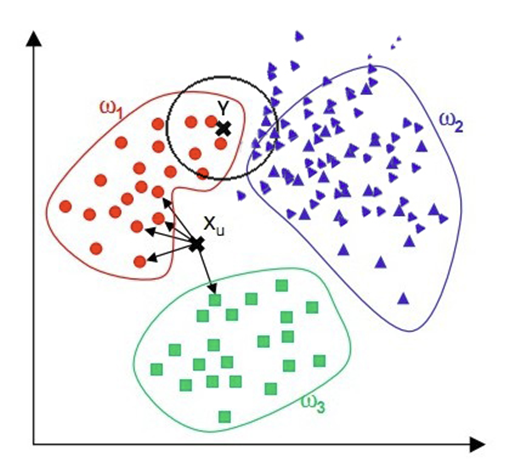
\includegraphics{06.png}
    
    该算法只计算最近的邻居样本,某一类的样本数量很大,那么或者这类样本并不接近目标样本,或者这类样本很靠近目标样本。无论怎样,数量并不能影响运行结果。可以采用权值的方法(和该样本距离小的邻居权值大)来改进。

    该方法的另一个不足之处是计算量较大,因为对每一个待分类的文本都要计算它到全体已知样本的距离,才能求得它的K个最近邻点。

可理解性差,无法给出像决策树那样的规则。

    K-means算法的缺点首先是在 K-means 算法中 K 是事先给定的,这个 K
值的选定是非常难以估计的。很多时候,事先并不知道给定的数据集应该分成多少个类别才最合适;其次,在
K-means
算法中,首先需要根据初始聚类中心来确定一个初始划分,然后对初始划分进行优化。这个初始聚类中心的选择对聚类结果有较大的影响,一旦初始值选择的不好,可能无法得到有效的聚类结果(如在问题二中选择不同的同学作为初始聚类中心,会有不同的聚类结果);最后,该算法需要不断地进行样本分类调整,不断地计算调整后的新的聚类中心,因此当数据量非常大时,算法的时间开销是非常大的。

\begin{itemize}
\item
  K-means算法对于不同的初始值,可能会导致不同结果。解决方法:

  \begin{itemize}
  \item
    多设置一些不同的初值,对比最后的运算结果,一直到结果趋于稳定结束
  \item
    很多时候,事先并不知道给定的数据集应该分成多少个类别才最合适。通过类的自动合并和分裂,得到较为合理的类型数目
    K,例如 ISODATA 算法。
  \end{itemize}
\item
  K-means算法的其他改进算法如下:
\end{itemize}

鉴于K-means算法和人工蜂群算法各自特性,提出一种基于改进人工蜂群的K-means聚类算法IABC-Kmeans。该算法首先对人工蜂群算法进行改进:利用提出的最大最小距离积法初始化蜂群,保证初始点的选择能够尽可能代表数据集的分布特征;在迭代过程中使用新的适应度函数和位置更新公式完成寻优进化。然后将改进后的人工蜂群算法应用到K-means算法中完成聚类。
\href{https://github.com/DMinerJackie/IABC-KMC}{论文及github地址}


    % Add a bibliography block to the postdoc
    
    
    
\end{document}
